% !Mode:: "TeX:UTF-8"
% !TEX encoding = UTF-8 Unicode

%----------------------------------------------------------------------------------------
% 机器翻译:统计建模与深度学习方法
% Machine Translation: Statistical Modeling and Deep Learning Methods
%
% Copyright 2020
% 肖桐(xiaotong@mail.neu.edu.cn) 朱靖波 (zhujingbo@mail.neu.edu.cn)
%----------------------------------------------------------------------------------------

%----------------------------------------------------------------------------------------
%    CONFIGURATIONS
%----------------------------------------------------------------------------------------

\renewcommand\figurename{图}%将figure改为图
\renewcommand\tablename{表}%将figure改为图
\definecolor{ublue}{rgb}{0.152,0.250,0.545}
\definecolor{ugreen}{rgb}{0,0.5,0}
\chapterimage{fig-NEU-7.jpg} % Chapter heading image

%----------------------------------------------------------------------------------------
%	CHAPTER 6
%----------------------------------------------------------------------------------------

\chapter{神经机器翻译模型}

\parinterval {\small\sffamily\bfseries{神经机器翻译}} \index{神经机器翻译}(Neural Machine Translation)\index{Neural Machine Translation}是机器翻译的前沿方法。近几年,随着深度学习技术的发展和在各领域中的深入应用,基于端到端表示学习的方法正在改变着我们处理自然语言的方式,神经机器翻译在这种趋势下应运而生。一方面,神经机器翻译仍然延续着统计建模和基于数据驱动的思想,因此在基本问题的定义上与前人的研究是一致的;另一方面,神经机器翻译脱离了统计机器翻译中对隐含翻译结构的假设,同时使用分布式表示来对文字序列进行建模,这使得它可以从一个全新的视角看待翻译问题。现在,神经机器翻译已经成为了机器翻译研究及应用的热点,译文质量得到了巨大的提升。本章将对神经机器翻译的基础模型和方法进行介绍。

%----------------------------------------------------------------------------------------
%    NEW SECTION
%----------------------------------------------------------------------------------------
\vspace{-0.7em}
\section{神经机器翻译的发展简史}

\parinterval 纵观机器翻译的发展历程,神经机器翻译诞生很晚。无论是早期的基于规则的方法,还是逐渐发展起来的基于实例的方法,再到上世纪末的统计方法,每次机器翻译框架级的创新都需要很长时间的酝酿,而技术走向成熟甚至需要更长的时间。但是,神经机器翻译的出现和后来的发展速度多少有些令人``出人意料''。神经机器翻译的概念出现在2013-2014年间,当时机器翻译领域的主流方法仍然是统计机器翻译。虽然那个时期深度学习已经在图像、语音等领域取得令人瞩目的效果,但是对于自然语言处理来说深度学习仍然不是主流。这也导致当时的研究者对神经机器翻译这种方法还有一些排斥。

\parinterval 不过,有人也意识到了神经机器翻译在表示学习等方面的优势。特别是,以Yoshua Bengio团队为代表的研究力量对包括机器翻译在内的序列到序列问题进行了广泛而深入的研究,注意力机制等新的模型不断被推出。这使得神经机器翻译系统在翻译品质上逐渐体现出优势,甚至超越了当时的统计机器翻译系统。正当大家在讨论神经机器翻译是否能取代统计机器翻译成为下一代机器翻译范式的时候,谷歌、百度等企业推出以神经机器翻译技术为内核的在线机器翻译服务,在很多场景下的翻译品质显著超越了当时最好的统计机器翻译系统。这也引发了学术界和产业界对神经机器翻译的讨论。随着关注度的不断升高,神经机器翻译的研究吸引了更多的科研机构和企业的投入,神经机器翻译系统的翻译品质得到进一步提升。

\parinterval 在短短5-6年间,神经机器翻译从一个新生的概念已经成长为机器翻译领域的最前沿技术之一,在各种机器翻译评测和应用中呈全面替代统计机器翻译之势。比如,从近几年WMT、CCMT等评测的结果来看,神经机器翻译已经处于绝对的统治地位,在不同语种和领域的翻译任务中,成为各参赛系统的标配。此外,从ACL等自然语言处理顶级会议的发表论文看,神经机器翻译是毫无疑问的焦点,在论文数量上呈明显的增长趋势,这也体现了学术界对该方法的热情。至今,无论是国外的著名企业,如谷歌、微软、脸书,还是国内的团队,如百度、腾讯、阿里巴巴、有道、搜狗、小牛翻译,都推出了自己研发的神经机器翻译系统,整个研究和产业生态欣欣向荣。图\ref{fig:6-1}展示了包含神经机器翻译在内的机器翻译发展简史。

%----------------------------------------------
\begin{figure}[htp]
\centering
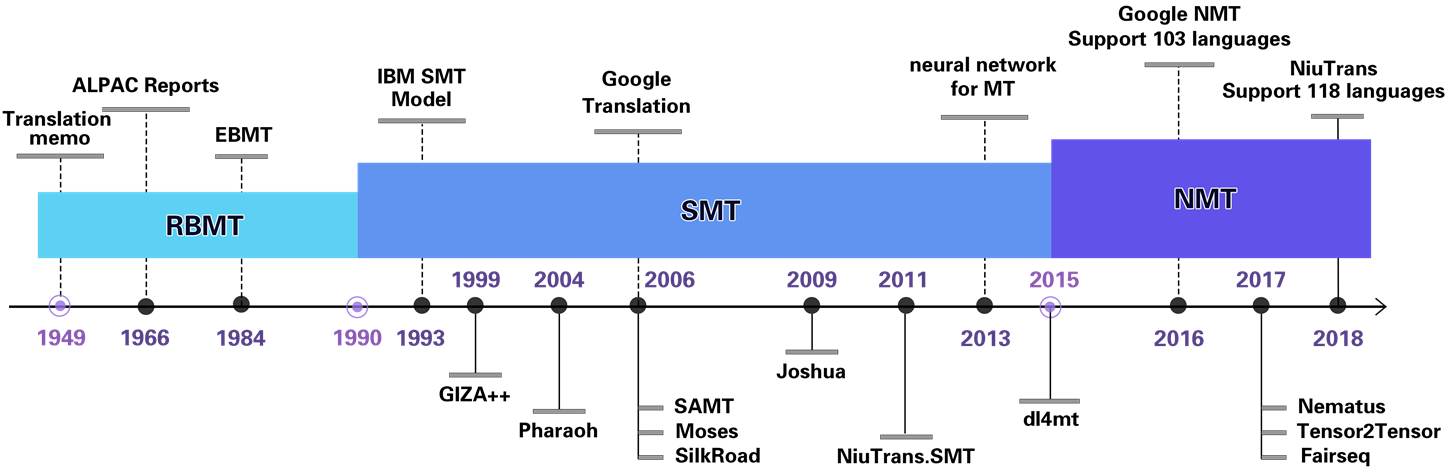
\includegraphics[scale=0.36]{./Chapter6/Figures/mt-history.png}
\caption{机器翻译发展简史}
\label{fig:6-1}
\end{figure}
%----------------------------------------------

\parinterval 神经机器翻译的迅速崛起确实让所有人都有些措手不及,甚至有一种一觉醒来天翻地覆的感觉。也有人评价,神经机器翻译的出现给整个机器翻译领域带来了前所未有的发展机遇。不过,客观地看,机器翻译达到今天这样的状态也是一种历史必然,其中有几方面原因:

\begin{itemize}
\vspace{0.3em}
\item 自上世纪末所发展起来的基于数据驱动的方法为神经机器翻译提供了很好的基础。本质上,神经机器翻译仍然是一种基于统计建模的数据驱动的方法,因此无论是对问题的基本建模方式,还是训练统计模型所使用到的带标注数据,都可以复用机器翻译领域以前的研究成果。特别是机器翻译长期的发展已经积累了大量的双语、单语数据,这些数据在统计机器翻译时代就发挥了很大作用。随着时间的推移,数据规模和质量又得到进一步提升,包括一些评测基准、任务设置都已经非常完备,研究者可以直接在数据条件全部具备的情况下开展神经机器翻译的研究工作,这些都省去了大量的时间成本。从这个角度说,神经机器翻译是站在巨人的肩膀上才发展起来的。
\vspace{0.3em}
\item 深度学习经过长时间的酝酿终于爆发,为机器翻译等自然语言处理任务提供了新的思路和技术手段。神经机器翻译的不断壮大伴随着深度学习技术的发展。在深度学习的视角下,语言文字可以被表示成抽象的实数向量。这种文字的表示方法可以被自动学习,为机器翻译建模提供了更大的灵活性。相对于神经机器翻译,深度学习的发展更加曲折。虽然深度学习经过了漫长的起伏过程,但是神经机器翻译恰好出现在深度学习逐渐走向成熟的阶段。反过来说,受到深度学习及相关技术空前发展的影响,自然语言处理的范式也发生了变化,神经机器翻译的出现只是这种趋势下的一种必然。
\vspace{0.3em}
\item 此外,计算机算力的提升也为神经机器翻译提供了很好的支撑。与很多神经网络方法一样,神经机器翻译也依赖大量的基于浮点数的矩阵运算。在2000年前,大规模的矩阵运算仍然依赖非常昂贵的CPU集群系统,但是随着GPU等相关技术的发展,在相对低成本的设备上已经可以完成非常复杂的浮点并行运算。这使得包括神经机器翻译在内的很多基于深度学习的系统可以进行大规模实验,随着实验周期的缩短,相关研究和系统的迭代周期大大缩短。实际上,计算机硬件运算能力一直是稳定提升的,神经机器翻译只是受益于运算能力的阶段性突破。
\vspace{0.3em}
\item 还有,翻译需求的不断增加也为机器翻译技术提供了新的机会。在近几年,无论是翻译品质,还是翻译语种数量,甚至不同的翻译场景,都对机器翻译有了更高的要求。人们迫切需要一种品质更高、翻译效果稳定的机器翻译方法,神经机器翻译恰好满足了这些要求。当然,应用端需求的增加也会反推机器翻译技术的发展,二者相互促进。
\vspace{0.3em}
\end{itemize}

\parinterval 至今,神经机器翻译已经成为带有时代特征的标志性方法。当然,机器翻译的发展也远没有达到终点。下面将介绍神经机器翻译的起源和优势,以便读者在正式了解神经机器翻译的技术方法前对其现状有一个充分的认识。

%----------------------------------------------------------------------------------------
%    NEW SUB-SECTION
%----------------------------------------------------------------------------------------
%\vspace{-0.3em}
\subsection{神经机器翻译的起源}

\vspace{0.3em}
\parinterval 从广义上讲,神经机器翻译是一种基于人工神经网络的方法,它把翻译过程描述为可以用人工神经网络表示的函数。所有的训练和推断都在这些函数上进行。由于神经机器翻译中的神经网络可以用连续可微函数表示,因此这类方法也可以用基于梯度的方法进行优化,相关技术非常成熟。更为重要的是,在神经网络的设计中,研究者引入了{\small\bfnew{分布式表示}} \index{分布式表示}(Distributed Representation)\index{Distributed Representation}的概念,这也是近些年自然语言处理领域的重要成果之一。传统统计机器翻译仍然把词序列看作离散空间里的由多个特征函数描述的点,类似于$n$-gram语言模型,这类模型对数据稀疏问题非常敏感。此外,人工设计特征也在一定程度上限制了模型对问题的表示能力。神经机器翻译把文字序列表示为实数向量,一方面避免了特征工程繁重的工作,另一方面使得系统可以对文字序列的``表示''进行学习。可以说,神经机器翻译的成功很大程度上源自`` 表示学习''这种自然语言处理的新范式的出现。在表示学习的基础上,注意力机制、深度神经网络等技术都被应用于神经机器翻译,使其得以进一步发展。

\parinterval 虽然神经机器翻译中大量的使用了人工神经网络方法,但是它并不是最早在机器翻译中使用人工神经网络的框架。实际上,人工神经网络在机器翻译中应用的历史要远早于现在的神经机器翻译。 在统计机器翻译时代,也有很多研究者利用人工神经网络进行机器翻译系统模块的构建\cite{devlin-etal-2014-fast,Schwenk_continuousspace},比如,Jacob Devlin等人就成功地在统计机器翻译系统中使用了基于神经网络的联合表示模型,取得了令人振奋的结果,这项工作也获得了ACL2014的最佳论文奖(Best Paper Award)。

\parinterval 不过,以上这些工作大多都是在系统的局部模块中使用人工神经网络和深度学习方法。与之不同的是,神经机器翻译是用人工神经网络完成整个翻译过程的建模,这样做的一个好处是,整个系统可以进行端到端学习,无需引入对任何翻译的隐含结构假设。这种利用端到端学习对机器翻译进行神经网络建模的方式也就成为了现在大家所熟知的神经机器翻译。这里简单列出部分代表性的工作:

\begin{itemize}
\vspace{0.3em}
\item 早在2013年,牛津大学的Nal Kalchbrenner和Phil Blunsom提出了一个基于编码器-解码器结构的新模型\cite{kalchbrenner-blunsom-2013-recurrent}。该模型用卷积神经网络(CNN)将源语言编码成实数向量,之后用循环神经网络(RNN)将连续向量转换成目标语言。这使得模型不需要进行词对齐、特征提取等工作,就能够自动学习源语言的信息。这也是一种端到端学习的方法。不过,这项工作的实现较复杂,而且方法存在梯度消失/爆炸等问题\cite{HochreiterThe,BENGIO1994Learning},因此并没有成为后来神经机器翻译的基础框架。
\vspace{0.3em}
\item 2014年,谷歌的Ilya Sutskever等人提出了序列到序列(seq2seq)学习的方法,同时将长短记忆结构(LSTM)引入到神经机器翻译中,这个方法解决了梯度爆炸/消失的问题,并且通过遗忘门的设计让网络选择性地记忆信息,缓解了序列中长距离依赖的问题\cite{NIPS2014_5346}。但是该模型在进行编码的过程中,将不同长度的源语言句子压缩成了一个固定长度的向量,句子越长,损失的信息越多,同时该模型无法对输入和输出序列之间的对齐进行建模,因此并不能有效的保证翻译质量。
\vspace{0.3em}
\item 同年Dzmitry Bahdanau等人首次将注意力机制(Attention Mechanism)应用到机器翻译领域,在机器翻译任务上对翻译和局部翻译单元之间的对应关系同时建模\cite{bahdanau2014neural}。Bahdanau等人工作的意义在于,使用了更加有效的模型来表示源语言的信息,同时使用注意力机制对两种语言不同部分之间的相互联系进行建模。这种方法可以有效地处理长句子的翻译,而且注意力的中间结果具有一定的可解释性\footnote{比如,目标语言和源语言句子不同单词之间的注意力强度能够在一定程度上反应单词之间的互译程度。} 。然而相比于前人的神经机器翻译模型,注意力模型也引入了额外的成本,计算量较大。
\vspace{0.3em}
\item 2016年谷歌发布了基于多层循环神经网络方法的GNMT系统。该系统集成了当时的神经机器翻译技术,并进行了诸多的改进。它的性能显著优于基于短语的机器翻译系统\cite{Wu2016GooglesNM},引起了研究者的广泛关注。在之后不到一年的时间里,Facebook采用卷积神经网络(CNN)研发了新的神经机器翻译系统\cite{DBLP:journals/corr/GehringAGYD17},实现了比基于循环神经网络(RNN)系统更高的翻译水平,并大幅提升翻译速度。
\vspace{0.3em}
\item 2017年,谷歌的Ashish Vaswani等人提出了新的翻译模型Transformer。其完全抛弃了CNN、RNN等结构,仅仅通过自注意力机制(Self-Attentiion)和前向神经网络,不需要使用序列对齐的循环框架就展示出强大的性能,并且巧妙的解决了翻译中长距离依赖问题\cite{NIPS2017_7181}。Transformer是第一个完全基于注意力机制搭建的模型,不仅训练速度更快,在翻译任务上也获得了更好的结果,一跃成为目前最主流的神经机器翻译框架。
\vspace{0.3em}
\end{itemize}

\parinterval  神经机器翻译的工作远不止以上这些内容,实际上全面介绍所有神经机器翻译的方法也是非常有挑战的工作。感兴趣的读者可以参考一篇关于神经机器翻译的综述文章\ \dash\ Neural Machine Translation: A Review\cite{StahlbergNeural}。本章会对神经机器翻译的典型方法进行细致的介绍。

%----------------------------------------------------------------------------------------
%    NEW SUB-SECTION
%----------------------------------------------------------------------------------------

\subsection{神经机器翻译的品质 }
\vspace{0.3em}
\parinterval  图\ref{fig:6-2}是一个真实的机器翻译的例子。其中译文1是统计机器翻译系统的结果,译文2是神经机器翻译系统的结果。为了保证公平性,两个系统使用完全相同的数据进行训练。

%----------------------------------------------
\begin{figure}[htp]
\centering
\begin{tikzpicture}
%第一段----------------------------------------------
%原文-------------
\node [pos=0.4,left,xshift=-36em,yshift=7.3em,font=\small] (original0) {原文:};
\node [pos=0.4,left,xshift=-2em,yshift=3.3em,font=\small] (original1) {
\begin{tabular}[t]{l}
\parbox{36em}{During Soviet times, if a city’s population topped one million, it would become eligible for its own metro. Planners wanted to brighten the lives of everyday Soviet citizens, and saw the metros, with their tens of thousands of daily passengers, as a singular opportunity to do so. In 1977, Tashkent, the capital of Uzbekistan, became the seventh Soviet city to have a metro built. Grand themes celebrating the history of Uzbekistan and the Soviet Union were brought to life, as art was commissioned and designers set to work. The stations reflected different themes, some with domed ceilings and painted tiles reminiscent of Uzbekistan’s Silk Road mosques, while others ...}
\end{tabular}
};
%译文1--------------mt1
\node[font=\small] (mt1) at ([xshift=0em,yshift=-9.1em]original0.south) {译文1:};
\node[font=\small] (ts1) at ([xshift=0em,yshift=-4em]original1.south)  {
\begin{tabular}[t]{l}
\parbox{36em}{在苏联时代,如果一个城市的人口突破一百万,这将成为合资格为自己的地铁。规划者想去照亮每天的苏联公民的生命,看到地铁,与他们的数十每天数千乘客,作为一个独特的机会来这样做。1977年,塔什干,乌兹别克斯坦的首都,成了苏联第七城市建有地铁。宏大主题,庆祝乌兹别克斯坦和苏联的历史被带到生活,因为艺术是委托和设计师开始工作。车站反映了不同的主题,有的圆顶天花板和绘瓷砖让人想起乌兹别克斯坦是丝绸之路的清真寺,而另一些则装饰着...}
\end{tabular}
};



%{
%\draw[dotted,thick,ublue] ([xshift=10.3em,yshift=0.3em]mt8.south west)--%([xshift=-5.2em,yshift=-0.3em]ht8.north);
%}



\begin{pgfonlayer}{background}
{
\node[rectangle,draw=ublue, inner sep=0mm] [fit =(original0)(mt1)(mt1)(ts1)(original1)] {};
}
\end{pgfonlayer}


\end{tikzpicture}
\setlength{\abovecaptionskip}{-0.2cm}
%\caption{机器翻译实例对比}
%\label{fig:6-2}
\end{figure}
%----------------------------------------------

%----------------------------------------------
\begin{figure}[htp]
\centering
\begin{tikzpicture}
%-------译文2
\node [pos=0.4,left,xshift=-36em,yshift=7.3em,font=\small] (original0) {译文2:};
\node [pos=0.4,left,xshift=-2em,yshift=4.5em,font=\small] (original1) {
\begin{tabular}[t]{l}
\parbox{36em}{在苏联时期,如果一个城市的人口超过一百万,它就有资格拥有自己的地铁。 规划者想要照亮日常苏联公民的生活,并把拥有数万名每日乘客的地铁看作是这样做的一个绝佳机会。 1977年,乌兹别克斯坦首都塔什干成为苏联第七个修建地铁的城市。 随着艺术的委托和设计师们的工作,乌兹别克斯坦和苏联历史的宏伟主题被赋予了生命力。 这些电台反映了不同的主题,有的有穹顶和彩砖,让人想起乌兹别克斯坦的丝绸之路清真寺,有的则用...}
\end{tabular}
};

\begin{pgfonlayer}{background}
{
\node[rectangle,draw=ublue, inner sep=0mm] [fit =(original0)(original1)] {};
}
\end{pgfonlayer}


\end{tikzpicture}
\setlength{\abovecaptionskip}{-0.2em}
\caption{机器翻译实例对比}
\label{fig:6-2}
\end{figure}
%----------------------------------------------
%----------------------------------------------
%\begin{figure}[htp]
%\centering
%\begin{tikzpicture}
%第一段----------------------------------------------
%原文-------------
\node [pos=0.4,left,xshift=-36em,yshift=7.3em,font=\small] (original0) {原文:};
\node [pos=0.4,left,xshift=-2em,yshift=3.3em,font=\small] (original1) {
\begin{tabular}[t]{l}
\parbox{36em}{During Soviet times, if a city’s population topped one million, it would become eligible for its own metro. Planners wanted to brighten the lives of everyday Soviet citizens, and saw the metros, with their tens of thousands of daily passengers, as a singular opportunity to do so. In 1977, Tashkent, the capital of Uzbekistan, became the seventh Soviet city to have a metro built. Grand themes celebrating the history of Uzbekistan and the Soviet Union were brought to life, as art was commissioned and designers set to work. The stations reflected different themes, some with domed ceilings and painted tiles reminiscent of Uzbekistan’s Silk Road mosques, while others ...}
\end{tabular}
};
%译文1--------------mt1
\node[font=\small] (mt1) at ([xshift=0em,yshift=-9.1em]original0.south) {译文1:};
\node[font=\small] (ts1) at ([xshift=0em,yshift=-4em]original1.south)  {
\begin{tabular}[t]{l}
\parbox{36em}{在苏联时代,如果一个城市的人口突破一百万,这将成为合资格为自己的地铁。规划者想去照亮每天的苏联公民的生命,看到地铁,与他们的数十每天数千乘客,作为一个独特的机会来这样做。1977年,塔什干,乌兹别克斯坦的首都,成了苏联第七城市建有地铁。宏大主题,庆祝乌兹别克斯坦和苏联的历史被带到生活,因为艺术是委托和设计师开始工作。车站反映了不同的主题,有的圆顶天花板和绘瓷砖让人想起乌兹别克斯坦是丝绸之路的清真寺,而另一些则装饰着...}
\end{tabular}
};

%译文2---------------mt2
\node[font=\small] (mt2) at ([xshift=0em,yshift=-6.7em]mt1.south) {译文2:};
\node[font=\small] (mt3) at ([xshift=0em,yshift=-4em]ts1.south)  {
\begin{tabular}[t]{l}
\parbox{36em}{在苏联时期,如果一个城市的人口超过一百万,它就有资格拥有自己的地铁。 规划者想要照亮日常苏联公民的生活,并把拥有数万名每日乘客的地铁看作是这样做的一个绝佳机会。 1977年,乌兹别克斯坦首都塔什干成为苏联第七个修建地铁的城市。 随着艺术的委托和设计师们的工作,乌兹别克斯坦和苏联历史的宏伟主题被赋予了生命力。 这些电台反映了不同的主题,有的有穹顶和彩砖,让人想起乌兹别克斯坦的丝绸之路清真寺,有的则用...}
\end{tabular}
};


%{
%\draw[dotted,thick,ublue] ([xshift=10.3em,yshift=0.3em]mt8.south west)--%([xshift=-5.2em,yshift=-0.3em]ht8.north);
%}



\begin{pgfonlayer}{background}
{
\node[rectangle,draw=ublue, inner sep=0mm] [fit =(original0)(mt1)(mt3)(mt1)(ts1)(mt2)(original1)] {};
}
\end{pgfonlayer}


\end{tikzpicture}
%\caption{机器翻译实例对比}
%\label{fig:6-2}
%\end{figure}
%----------------------------------------------

\vspace{-0.3em}
\parinterval  可以明显地看到译文2更加通顺,意思的表达更加准确,翻译质量明显高于译文1。这个例子基本反应出统计机器翻译和神经机器翻译的差异性。当然,这里并不是要讨论统计机器翻译和神经机器翻译孰优孰劣。但是,很多场景中都不难发现神经机器翻译可以生成非常流畅的译文,易于人工阅读和修改。

\parinterval  在很多量化的评价中也可以看到神经机器翻译的优势。回忆一下第一章提到的机器翻译质量的自动评估指标中,使用最广泛的一种指标是BLEU。在统计机器翻译时代,在由美国国家标准和科技机构(NIST)举办的汉英机器翻译评测中(比如汉英MT08数据集),基于统计方法的翻译系统能够得到30\%以上的BLEU值已经是当时最顶尖的结果了。而现在的神经机器翻译系统,则可以轻松的将BLEU提高至45\%以上。

%----------------------------------------------
\begin{figure}[htp]
\centering
% not compatible with [scale=?]


%----------------------------------------------------  
  
    \begin{tikzpicture}
        \begin{scope}[local bounding box=WMT]
            \draw[->,thick] (0.4,0) to (9.5,0);
            \draw[->,thick] (0.4,-0) to (0.4,4.3);
            \draw[thick] (0.4,2) to (0.6,2);
            \draw[thick] (0.4,4) to (0.6,4);
            \node[font=\scriptsize] at (0,2) {10};
            \node[font=\scriptsize] at (0,4) {20};

            % 2015
            \node[minimum width=0.5cm,thick,minimum height=7*0.2cm,fill=blue!30!white,inner sep=0pt,outer sep=0pt,anchor=south west] (smt2015) at (1.5*0.7,0.5pt) {};
            \node[minimum width=0.5cm,thick,minimum height=2*0.2cm,fill=red!30!white,inner sep=0pt,outer sep=0pt,anchor=south west] (nmt2015) at (smt2015.south east) {};
            \node[font=\scriptsize,anchor=north] () at ([yshift=-0.2em]smt2015.south east) {2015};
            % 2016
            \node[minimum width=0.5cm,thick,minimum height=3*0.2cm,fill=blue!30!white,inner sep=0pt,outer sep=0pt,anchor=south west] (smt2016) at ($(nmt2015.south east)+(0.7,0)$) {};
            \node[minimum width=0.5cm,thick,minimum height=8*0.2cm,fill=red!30!white,inner sep=0pt,outer sep=0pt,anchor=south west] (nmt2016) at (smt2016.south east) {};
            \node[font=\scriptsize,anchor=north] () at ([yshift=-0.2em]smt2016.south east) {2016};
            % 2017
            \node[minimum width=0.5cm,thick,minimum height=3*0.2cm,fill=blue!30!white,inner sep=0pt,outer sep=0pt,anchor=south west] (smt2017) at ($(nmt2016.south east)+(0.7,0)$) {};
            \node[minimum width=0.5cm,thick,minimum height=13*0.2cm,fill=red!30!white,inner sep=0pt,outer sep=0pt,anchor=south west] (nmt2017) at (smt2017.south east) {};
            \node[font=\scriptsize,anchor=north] () at ([yshift=-0.2em]smt2017.south east) {2017};
            % 2018
            \node[minimum width=0.5cm,thick,minimum height=0cm,draw,fill=blue!30!white,inner sep=0pt,outer sep=0pt,anchor=south west] (smt2018) at ($(nmt2017.south east)+(0.7,0)$) {};
            \node[minimum width=0.5cm,thick,minimum height=14*0.2cm,fill=red!30!white,inner sep=0pt,outer sep=0pt,anchor=south west] (nmt2018) at (smt2018.south east) {};
            \node[font=\scriptsize,anchor=north] () at ([yshift=-0.2em]smt2018.south east) {2018};
             % 2019
            \node[minimum width=0.5cm,thick,minimum height=0cm,draw,fill=blue!30!white,inner sep=0pt,outer sep=0pt,anchor=south west] (smt2019) at ($(nmt2018.south east)+(0.7,0)$) {};
            \node[minimum width=0.5cm,thick,minimum height=21*0.2cm,fill=red!30!white,inner sep=0pt,outer sep=0pt,anchor=south west] (nmt2019) at (smt2019.south east) {};
            \node[font=\scriptsize,anchor=north] () at ([yshift=-0.2em]smt2019.south east) {2019};
        \end{scope}

        % legend
        \ExtractX{$(nmt2015.west)$}
        \ExtractY{$(WMT.north)$}
        \node[minimum width=0.5cm,rectangle,fill=blue!30!white,anchor=north west,label={[label distance=1pt,font=\scriptsize]0:统计机器翻译}] () at (\XCoord,\YCoord) {};
        \ExtractX{$(nmt2017.west)$}
        \node[minimum width=0.5cm,rectangle,fill=red!30!white,anchor=north west,label={[label distance=1pt,font=\scriptsize]0:神经机器翻译}] () at (\XCoord,\YCoord) {};

  
       % \node[font=\normalsize,rotate=90] () at ([xshift=-1em]WMT.west) {数量};
       \node[font=\normalsize] () at (0.4,4.5) {数量};
        \node[font=\normalsize] () at (9.5,-0.3) {年份};
        
        
    \end{tikzpicture}

\caption{WMT冠军系统的数量}
\label{fig:6-3}
\end{figure}
%----------------------------------------------

\parinterval  同样,在机器翻译领域中最具影响力的评测比赛WMT(Workshop of Machine Translation)中,使用统计机器翻译方法的参赛系统也在逐年减少。而现在获得比赛冠军的系统中几乎没有只使用纯统计机器翻译模型的系统\footnote{但是,仍然有大量的统计机器翻译和神经机器翻译融合的方法。比如,在无指导机器翻译中,统计机器翻译仍然被作为初始模型。} 。图\ref{fig:6-3}展示了近年来WMT比赛冠军系统中神经机器翻译系统的占比,可见神经机器翻译系统的占比在逐年提高。

%----------------------------------------------
\begin{figure}[htp]
\centering

%\definecolor{ublue}{rgb}{0.152,0.250,0.545}
\begin{tikzpicture}
\begin{axis}[ 
width=10cm, height=5cm, 
symbolic x coords={1-15,16-25,26-35,>35},
xtick=data,
ytick={6,12,...,28},
xlabel={句子长度(范围)},
ylabel={$\%$\footnotesize{mTER}},
xlabel style={align=center},
ylabel style={},
y tick style={opacity=0},
x tick label style={font=\small},
y tick label style={font=\small},
tick align=inside,
%major grid style={draw=blue,dashed},
legend pos=outer north east,
%legend style={anchor=north west,yshift=-1cm},
legend style={yshift=-4.5em,xshift=-6em,legend cell align=left,legend plot pos=right},
ymin=6,
ymax=28]
\addplot [sharp plot,very thick,ublue,mark=diamond*] coordinates{(1-15,11.3) (16-25,16.4) (26-35,17) (>35,19.8)};
\addplot [sharp plot,very thick,red,mark=triangle*] coordinates{(1-15,14.4) (16-25,22.6) (26-35,23.8) (>35,25.9)};
\addplot [sharp plot,very thick,ugreen,mark=square*] coordinates{(1-15,14.9) (16-25,23.7) (26-35,24.7) (>35,26.4)};
\addplot [sharp plot,very thick,orange,mark=*] coordinates{(1-15,17.5) (16-25,24) (26-35,25) (>35,27)};
\legend{\tiny{NMT},\tiny{SPB},\tiny{HPB},\tiny{PBSY}} 
\end{axis}
\end{tikzpicture}

%---------------------------------------------------------------------

\caption{不同系统在不同长度句子上的mTER分值(得分越低越好)}
\label{fig:6-4}
\end{figure}
%----------------------------------------------

\parinterval  除了上面例子中展示的流畅度和准确度外,神经机器翻译在其他评价指标上的表现也全面超越统计机器翻译\cite{Bentivogli2016NeuralVP}。比如,在IWSLT 2015英语-德语任务中,与三个最先进的统计机器翻译系统(PBSY、HPB、SPB)相比,神经机器翻译系统的mTER得分在不同长度句子上都有明显的下降,如图\ref{fig:6-4}\footnote{mTER是一种错误率度量,值越低表明译文越好。}。其次,神经机器翻译的单词形态错误率和单词词义错误率都远低于统计机器翻译系统(表\ref{tab:6-1} )。

\vspace{0.5em}%全局布局使用
%----------------------------------------------
\begin{table}[htp]
\centering
\caption{NMT与SMT系统的译文错误率\cite{Bentivogli2016NeuralVP}}
\label{tab:6-1}
\begin{tabular}{r|llc}
system                    & word & lemma & \%Δ \\ \hline
PBSY                    &27.1          & 22.5           & -16.9       \\
HPB                     & 28.7          & 23.5           & -18.4       \\
SPB                     & 28.3          & 23.2           & -18.0       \\
NMT                     & $ 21.7^{\ast}$          & $18.7^{\ast}$           & -13.7      \\
\end{tabular}
\end{table}
%----------------------------------------------

\parinterval 更振奋人心的是,神经机器翻译在某些任务上的结果已经相当惊艳,比如在汉英新闻翻译任务中,神经机器翻译就取得了至少和专业翻译人员相媲美的效果\cite{Hassan2018AchievingHP}。在该任务中,神经机器系统(Combo-4、Combo-5 和 Combo-6)的人工评价得分与Reference-HT(专业翻译人员翻译)的得分无显著差别,且远超Reference-WMT(WMT的参考译文,也是由人类翻译)得分(表\ref{tab:6-2})。

\vspace{0.5em}%全局布局使用
%----------------------------------------------
\begin{table}[htp]
\centering
\caption{不同机器翻译系统人类评价结果\cite{Hassan2018AchievingHP}}
\label{tab:6-2}
\begin{tabular}{l | l l}
	\# 		&\begin{tabular}[c]{@{}l@{}}Ave\%\\ (平均原始分数)\end{tabular}		&System \\ \hline
	1 		&69.0			&Combo-6 \\
			&68.5			&Reference-HT \\
			&68.9			&Combo-5 \\
			&68.6			&Combo-4 \\
	2		&62.1			&Reference-WMT \\
\end{tabular}
\end{table}
%----------------------------------------------

\parinterval  在最近两年,神经机器翻译的发展更加迅速,新的模型、方法层出不穷。表\ref{tab:6-3}给出了2019年一些主流的神经机器翻译模型的对比\cite{WangLearning}。可以看到,相比2017年,2018-2019年中机器翻译仍然有明显的进步。

\vspace{0.5em}%全局布局使用
%----------------------------------------------
\begin{table}[htp]
\centering
\caption{WMT14英德数据集上不同神经机器翻译系统的表现\cite{WangLearning}}
\label{tab:6-3}
\begin{tabular}{ l | l l l}
   模型         		 &作者	& 年份	& BLEU \\ \hline
   ConvS2S                			&Gehring等 		&2017 			&25.2 \\
   Transformer-Base 			&Vaswani等 		&2017 			&27.3 \\
   Transformer-Big   			&Vaswani等 		&2017 			&28.4 \\
   RNMT+					&Chen等 	  	&2018  			&28.5 \\
   Layer-Wise Coordination 	&Xu等 	 		&2018 			&29 \\
   Transformer-RPR		 	&Shaw等 	 	&2018 			&29.2 \\
   Transformer-DLCL			 &Wang等 	 	&2019 			&29.3 \\
\end{tabular}
\end{table}
%----------------------------------------------

%----------------------------------------------------------------------------------------
%    NEW SUB-SECTION
%----------------------------------------------------------------------------------------

\subsection{神经机器翻译的优势 }

\vspace{1em}%全局布局使用
%----------------------------------------------
\begin{table}[htp]
\centering
\caption{统计机器翻译 vs 神经机器翻译}
\label{tab:6-4}
\begin{tabular}{ l | l }
  \rule{0pt}{15pt}  \parbox{12em}{统计机器翻译		}	&神经机器翻译\\ \hline
	  \rule{0pt}{13pt}  基于离散空间的表示模型			&基于连续空间的表示模型 \\
	  \rule{0pt}{13pt} NLP问题的隐含结构假设			&无隐含结构假设,端到端学习 \\
	  \rule{0pt}{13pt} 特征工程为主					&无显性特征,但需要设计网络 \\
	  \rule{0pt}{13pt} 特征、规则的存储耗资源			&模型存储相对小,但计算慢 \\
\end{tabular}
\end{table}
%----------------------------------------------

\parinterval  既然神经机器翻译如此强大,它的优势在哪里呢?为了回答这个问题,表\ref{tab:6-4}给出了神经机器翻译与统计机器翻译的简单对比。具体来说,神经机器翻译有如下特点:

\vspace{0.5em}
\parinterval  (一)分布式连续空间表示模型,能捕获更多隐藏信息

\parinterval  神经机器翻译与统计机器翻译最大的区别在于对语言文字串的表示方法上。在统计机器翻译中,所有词串本质上都是由更小的词串(短语、规则)组合而成,也就是统计机器翻译模型利用了词串之间的组合性来表示更大的词串。统计机器翻译使用多个特征描述翻译结果,但是其仍然对应着离散的字符串的组合,因此可以把模型对问题的表示空间看做是由一个离散结构组成的集合。在神经机器翻译中,词串的表示已经被神经网络转化为多维实数向量,而且也不依赖任何的可组合性假设等其他假设来刻画离散的语言结构,从这个角度说,所有的词串分别对应了一个连续空间上的点(比如,对应$n$维实数空间中一个点)。这样,模型可以更好地进行优化,而且对未见样本有更好的泛化能力。此外,基于连续可微函数的机器学习算法已经相对完备,可以很容易的对问题进行建模和优化。

\vspace{0.5em}
\parinterval  (二)不需要特征工程,特征学习更加全面

\parinterval  经典的统计机器翻译可以通过判别式模型引入任意特征,不过这些特征需要人工设计,因此这个过程也被称为{\small\bfnew{特征工程}} \index{特征工程}(Feature Engineering)\index{Feature Engineering}。特征工程依赖大量的人工,特别是对不同语种、不同场景的翻译任务,所采用的特征可能不尽相同,这也使得设计有效的特征成为了统计机器翻译时代最主要的工作之一。但是,由于人类自身的思维和认知水平的限制,人工设计的特征可能不全面,甚至会遗漏一些重要的翻译现象。神经机器翻译并不依赖任何人工特征的设计,或者说它的特征都隐含在分布式表示中。这些``特征''都是自动学习得到的,因此神经机器翻译并不会受到人工思维的限制,学习到的特征对问题描述更加全面。

\vspace{0.5em}
\parinterval  (三)不含隐含结构假设,端到端学习对问题建模更加直接

\parinterval  传统的自然语言处理任务会对问题进行隐含结构假设。比如,进行翻译时,统计机器翻译会假设翻译过程由短语的拼装完成。这些假设可以大大化简问题的复杂度,但是另一方面也带来了各种各样的约束条件。错误的隐含假设往往会导致建模错误。神经机器翻译是一种端到端模型,它并不依赖任何隐含结构假设。这样,模型并不会受到错误的隐含结构的引导。从某种意义上说,端到端学习可以让模型更加`` 自由''地进行学习,因此往往可以学到很多传统认知上不容易理解或者不容易观测到的现象。

\vspace{0.5em}
\parinterval  (四)模型结构统一,存储消耗更小

\parinterval  统计机器翻译系统依赖于很多模块,比如词对齐、短语(规则)表、目标语言模型等等,因为所有的信息(如$n$-gram)都是离散化表示的,因此模型需要消耗大量的存储资源。同时,由于系统模块较多,开发的难度也较大。神经机器翻译的模型都是用神经网络进行表示,模型参数大多是实数矩阵,因此存储资源的消耗很小。而且神经网络可以作为一个整体进行开发和调试,系统搭建的代价相对较低。实际上,由于模型体积小,神经机器翻译也非常合适于离线小设备上的翻译任务。

\vspace{0.5em}
\parinterval  当然,神经机器翻译也并不完美,很多问题有待解决。首先,神经机器翻译需要大规模浮点运算的支持,模型的推断速度较低。为了获得优质的翻译结果,往往需要大量GPU设备的支持,计算资源成本很高;其次,由于缺乏人类的先验知识对翻译过程的指导,神经机器翻译的运行过程缺乏可解释性,系统的可干预性也较差;此外,虽然脱离了繁重的特征工程,神经机器翻译仍然需要人工设计网络结构,包括在模型的各种超参的设置、训练策略的选择等方面,仍然需要大量人工参与。这也导致很多实验结果不容易重现。显然,完全不依赖人工进行机器翻译还很遥远。不过,随着研究者的不断攻关,很多问题也得到了解决。

%----------------------------------------------------------------------------------------
%    NEW SECTION
%----------------------------------------------------------------------------------------

\sectionnewpage
\section{编码器-解码器框架}

\parinterval 说到神经机器翻译就不得不提{\small\bfnew{编码器-解码器模型}}\index{编码器-解码器模型}(Encoder-Decoder Paradigm)\index{Encoder-Decoder Paradigm},或{\small\bfnew{编码器-解码器框架}} \index{编码器-解码器框架}。本质上,编码器-解码器模型是描述输入-输出之间关系的一种方式。编码器-解码器这个概念在日常生活中并不少见。例如在电视系统上为了便于视频的传播,会使用各种编码器将视频编码成数字信号,在客户端,相应的解码器组件会把收到的数字信号解码为视频。另外一个更贴近生活的例子是电话,它通过对声波和电信号进行相互转换,达到传递声音的目的。这种``先编码,再解码''的思想被应用到密码学、信息论等多个领域。

\parinterval 不难看出,机器翻译问题也完美的贴合编码器-解码器结构的特点。可以将源语言编码为类似信息传输中的数字信号,然后利用解码器对其进行转换,生成目标语言。下面就来看一下神经机器翻译是如何在编码器-解码器框架下进行工作的。

%----------------------------------------------------------------------------------------
%    NEW SUB-SECTION
%----------------------------------------------------------------------------------------

\subsection{框架结构}
\parinterval  编码器-解码器框架是一种典型的基于``表示''的模型。编码器的作用是将输入的文字序列通过某种转换变为一种新的``表示''形式,这种``表示''包含了输入序列的所有信息。之后,解码器把这种``表示''重新转换为输出的文字序列。这其中的一个核心问题是表示学习,即:如何定义对输入文字序列的表示形式,并自动学习这种表示,同时应用它生成输出序列。一般来说,不同的表示学习方法可以对应不同的机器翻译模型,比如,在最初的神经机器翻译模型中,源语言句子都被表示为一个独立的向量,这时表示结果是静态的;而在注意力机制中,源语言句子的表示是动态的,也就是翻译目标语的每个单词时都会使用不同的表示结果。

\parinterval  图\ref{fig:6-5}是一个应用编码器-解码器结构来解决机器翻译问题的简单实例。给定一个中文句子``我\ 对\ 你\ 感到\ 满意'',编码器会将这句话编码成一个实数向量(0.2,-1,6,5,0.7,-2),这个向量就是源语言句子的``表示''结果。虽然有些不可思议,但是神经机器翻译模型把这个向量等同于输入序列。向量中的数字并没有实际的意义,然而解码器却能从中提取到源语句子中所包含的信息。也有研究者把向量的每一个维度看作是一个``特征'',这样源语言句子就被表示成多个``特征''的联合,而且这些特征可以被自动学习。有了这样的源语言句子的``表示'',解码器可以把这个实数向量作为输入,然后逐词生成目标语句子``I am satisfied with you''。

%----------------------------------------------
\begin{figure}[htp]
\centering
\begin{tikzpicture}

\begin{scope}
\small{
\node [anchor=south west,minimum width=15em] (source) at (0,0) {\textbf{源语言}: \ \ 我\ \ \ \ 对\ \ \ \ 你\ \ \ \ 感到\ \ \ \ 满意 \ \ };
{
\node [anchor=south west,minimum width=15em] (target) at ([yshift=12em]source.north west) {\textbf{目标语言}: I\ \ am\ \ \ satisfied\ \ \ with\ \ \ you};
}
{
\node [anchor=center,minimum width=9.6em,minimum height=1.8em,draw,rounded corners=0.3em] (hidden) at ([yshift=6em]source.north) {};
\node [anchor=west,minimum width=1.5em,minimum size=1.5em,fill=ugreen!20] (cell01) at ([xshift=0.2em]hidden.west) {\footnotesize{.2}};
\node [anchor=west,minimum width=1.5em,minimum size=1.5em,fill=ugreen!10] (cell02) at (cell01.east) {\footnotesize{-1}};
\node [anchor=west,minimum width=1.5em,minimum size=1.5em,fill=ugreen!70] (cell03) at (cell02.east) {\footnotesize{6}};
\node [anchor=west,minimum width=1.5em,minimum size=1.5em,fill=ugreen!50] (cell04) at (cell03.east) {\footnotesize{5}};
\node [anchor=west,minimum width=1.5em,minimum size=1.5em,fill=ugreen!30] (cell05) at (cell04.east) {\footnotesize{.7}};
\node [anchor=west,minimum width=1.5em,minimum size=1.5em,fill=ugreen!10] (cell06) at (cell05.east) {\footnotesize{-2}};
}

%占位
\node (cell010) at ([xshift=-9em,yshift=0em]cell01.west){\quad};

%\rightarrow {}
\node [anchor=west,minimum width=1.5em,minimum size=1.5em] (cell07) at (cell06.east) {\hspace{0.07em}\footnotesize{$\longrightarrow$}};
\node [anchor=west,minimum width=1.5em,minimum size=1.5em] (cell08) at (cell06.east){\small{
\hspace{0.6em}
\begin{tabular}{l}
源语言句子的“表示”
\end{tabular}
}
};


{
\filldraw [fill=red!20,draw=white] (source.north west) -- (source.north east) -- ([xshift=-0.2em,yshift=-0.1em]hidden.south east) -- ([xshift=0.2em,yshift=-0.1em]hidden.south west);
}
{
\filldraw [fill=blue!20,draw=white] (target.south west) -- (target.south east) -- ([xshift=-0.2em,yshift=0.1em]hidden.north east) -- ([xshift=0.2em,yshift=0.1em]hidden.north west);
}
{
\draw [->,thick] (source.north west) -- ([xshift=0.2em,yshift=-0.1em]hidden.south west);
\draw [->,thick] (source.north east) -- ([xshift=-0.2em,yshift=-0.1em]hidden.south east);
}
{
\draw [->,thick] ([xshift=0.2em,yshift=0.1em]hidden.north west) -- (target.south west);
\draw [->,thick] ([xshift=-0.2em,yshift=0.1em]hidden.north east) -- (target.south east);
}
}

{
\node [anchor=south] (enclabel) at ([yshift=2em]source.north) {\small{\textbf{编码器(Encoder)}}};


\node [anchor=north] (declabel) at ([yshift=-2em]target.south) {\small{\textbf{解码器(Decoder)}}};
}



\end{scope}

\end{tikzpicture}
\caption{ Encoder-Decoder过程 }
\label{fig:6-5}
\end{figure}
%----------------------------------------------

\parinterval  在源语言句子的表示形式确定之后,需要设计相应的编码器和解码器结构。在大多数情况下,神经机器翻译系统中的编码器由词嵌入层和中间网络层组成。当输入一串单词序列时,词嵌入层会将以一维空间表示的离散的单词映射到连续的多维表示空间,这个过程也被称为词嵌入。之后中间层会对词嵌入向量进行更深层的抽象,得到输入单词序列的中间表示。中间层的实现方式有很多,比如:循环神经网络、卷积神经网络、Transformer等模型都是常用的结构。解码器的结构基本上和编码器是一致的,只不过多了输出层,用于输出每个目标语位置的单词生成概率。

\parinterval  现在,编码器-解码器框架已经成为了神经机器翻译系统的标准架构。当然,也有一些研究工作在探索编码器-解码器框架之外的结构\cite{Li2020NeuralMT},但是还没有太多颠覆性的进展。因此,本章仍然以编码器-解码器框架为基础对相关模型和方法进行介绍。

%----------------------------------------------------------------------------------------
%    NEW SUB-SECTION
%----------------------------------------------------------------------------------------

\subsection{表示学习}

\parinterval 编码器-解码器框架的创新之处在于,将传统基于符号的离散型知识转化为分布式的连续型知识。比如,对于一个句子,它可以由离散的符号所构成的文法规则来生成,也可以直接被表示为一个实数向量记录句子的各个``属性''。这种分布式的实数向量可以不依赖任何离散化的符号系统,简单来说,它就是一个函数,把输入的词串转化为实数向量。更为重要的是,这种分布式表示可以被自动学习。或者从某种意义上说,编码器-解码器框架的作用之一就是学习输入序列的表示。表示结果学习的好与坏很大程度上会影响神经机器翻译系统的性能。

\parinterval 图\ref{fig:6-6}形象地对比了统计机器翻译和神经机器翻译的表示模型的区别。传统的统计机器翻译(a)通过短语或者规则组合来获得更大的翻译片段,直至覆盖整个句子。这本质上是在一个离散的结构空间中不断组合的过程。神经机器翻译(b)与之不同,它并没有所谓的``组合''的过程,整个句子的处理是直接在连续空间上进行计算得到的。这二者的区别也体现了符号系统与神经网络系统的区别。前者更适合处理离散化的结构表示,后者更适合处理连续化的表示。

%----------------------------------------------
\begin{figure}[htp]
    \centering
    \begin{tikzpicture}

\begin{scope}
\node [anchor=south west,draw,thick,red,minimum width=0.9in,minimum height=0.7in] (space1) at (0,0) {};
\node [anchor=south west,fill=blue,minimum width=0.1in,minimum height=0.1in] (unit1) at (0.2,0.8) {};
\node [anchor=south west,fill=ugreen,minimum width=0.1in,minimum height=0.1in] (unit2) at (0.7,0.3) {};
\node [anchor=south west,fill=blue,minimum width=0.1in,minimum height=0.1in] (unit3) at (1.3,1.3) {};
\node [anchor=south west,fill=ugreen,minimum width=0.1in,minimum height=0.1in] (unit4) at ([xshift=0.1em]unit3.south east) {};

\begin{pgfonlayer}{background}
\node [rectangle,inner sep=2pt,rounded corners=1pt,draw,thick] [fit = (unit3) (unit4)] (unitbox) {};
\end{pgfonlayer}

\draw [->] ([yshift=1pt]unit1.north) .. controls +(north:0.23) and +(west:0.2) .. ([yshift=0.2em,xshift=-1pt]unitbox.west);
\draw [->] ([xshift=1pt]unit2.east) .. controls +(east:0.5) and +(south:0.2) .. ([xshift=0.2em,yshift=-1pt]unitbox.south);

\node [anchor=south] (spacelabel1) at (space1.north) {\scriptsize{离散表示空间}};
\node [anchor=north] (captain1) at ([yshift=-0.5em]space1.south) {\small{(a) \textbf{统计机器翻译}}};

\end{scope}

\begin{scope}[xshift=1.8in]
\node [anchor=south west,draw,thick,red,minimum width=0.9in,minimum height=0.7in] (space1) at (0,0) {};
\node [anchor=south west,fill=blue,minimum width=0.1in,minimum height=0.1in] (unit1) at (0.2,0.8) {};
\node [anchor=south west,fill=ugreen,minimum width=0.1in,minimum height=0.1in] (unit2) at (0.7,0.3) {};

\node [anchor=south west,draw,thick,red,minimum width=0.9in,minimum height=0.7in] (space2) at (1.3in,0) {};
\node [anchor=south west,circle,fill=orange,minimum width=0.1in,minimum height=0.1in] (unit3) at (1.7in,1.3) {};

\draw [->] ([yshift=1pt]unit1.north) .. controls +(north:0.4) and +(west:2) .. ([yshift=0.0em,xshift=-1pt]unit3.west);
\draw [->] ([xshift=1pt]unit2.east) .. controls +(east:1.5) and +(south:1) .. ([xshift=0.0em,yshift=-1pt]unit3.south);

\node [anchor=south] (spacelabel1) at (space1.north) {\scriptsize{离散表示空间}};
\node [anchor=south] (spacelabel2) at (space2.north) {\scriptsize{连续表示空间}};
\node [anchor=north] (captain1) at ([yshift=-0.5em,xshift=1em]space1.south east) {\small{(b) \textbf{神经机器翻译}}};

\end{scope}

\end{tikzpicture}
    \caption{统计机器翻译和神经机器翻译的表示空间}
    \label{fig:6-6}
\end{figure}
%----------------------------------------------

\parinterval 实际上,编码器-解码器模型也并不是表示学习实现的唯一途径。比如,在第五章提到的神经语言模型实际上也是一种有效的学习句子表示的方法,它所衍生出的预训练模型可以从大规模单语数据上学习句子的表示形式。这种学习会比使用少量的双语数据进行编码端和解码端的学习更加充分。相比机器翻译任务,语言模型相当于一个编码器的学习 \footnote{相比神经机器翻译的编码器,神经语言模型会多出一个输出层,这时可以直接把神经语言模型的中间层的输出作为编码器的输出。},可以无缝嵌入到神经机器翻译模型中。不过,值得注意的是,机器翻译的目的是解决双语字符串之间的映射问题,因此它所使用的句子表示是为了更好地进行翻译。从这个角度说,机器翻译中的表示学习又和语言模型中的表示学习有不同。不过,这里不会深入讨论神经语言模型和预训练与神经机器翻译之间的异同,感兴趣的读者可以参看第五章的相关内容。

\parinterval 还有一点,在神经机器翻译中,句子的表示形式可以有很多选择。使用单个向量表示一个句子是一种最简单的方法。当然,也可以用矩阵、高阶张量完成表示。甚至,在解码时动态地生成源语言的表示结果。这部分技术也会在随后的内容中进行介绍。

%----------------------------------------------------------------------------------------
%    NEW SUB-SECTION
%----------------------------------------------------------------------------------------

\subsection{简单的运行实例}\label{chapter6.2.3}

\parinterval 为了对编码器-解码器框架和神经机器翻译的运行过程有一个直观的认识,这里演示一个简单的翻译实例。这里采用标准的循环神经网络作为编码器和解码器的结构。假设系统的输入和输出为:

\vspace{0.5em}
\parinterval  \hspace{5em} 源语(中文)输入:\{``我'',\ ``很'',\ ``好'',\ ``<eos>''\}

\vspace{0.3em}
\parinterval  \hspace{5em} 目标语(英文)输出:\{``I'',\ ``am'',\ ``fine'',\ ``<eos>''\}
\vspace{0.5em}

\noindent 其中,<eos>(End of Sequence)表示序列的终止,<sos>(Start of Sequence)表示序列的开始。

%----------------------------------------------
\begin{figure}[htp]
\centering
  \begin{tikzpicture}
   
        \setlength{\base}{1cm}

        \tikzstyle{rnnnode} = [rounded corners=1pt,minimum size=0.5\base,draw,inner sep=0pt,outer sep=0pt]
        \tikzstyle{wordnode} = [font=\footnotesize]

        % RNN translation model
        \begin{scope}[local bounding box=RNNMT]
            % RNN Encoder
            \coordinate (eemb0) at (0,0);
            \foreach \x [count=\y from 0] in {1,2,...,4}
                \node[rnnnode,minimum height=0.5\base,fill=green!30!white,anchor=west] (eemb\x) at ([xshift=0.4\base]eemb\y.east) {};
            \foreach \x in {1,2,...,4}
                \node[rnnnode,fill=blue!30!white,anchor=south] (enc\x) at ([yshift=0.5\base]eemb\x.north) {};
            \node[wordnode,left=0.4\base of enc1,font=\footnotesize] (init) {0};
 			\node[wordnode,anchor=east] (init2) at ([xshift=-3.0em]init.west){};
               {
                \node[rnnnode,fill=purple] (repr) at (enc4) {};
                \node[wordnode] (label) at ([yshift=2.5em]enc4.north) {
                \begin{tabular}{c}
                源语言句\\子表示
                \end{tabular}
                };
                \draw[->,dashed,thick] (label.south) -- (enc4.north);
            }

            \node[wordnode,below=0pt of eemb1,font=\footnotesize] (encwordin1) {我};
            \node[wordnode,below=0pt of eemb2,font=\footnotesize] (encwordin2) {很};
            \node[wordnode,below=0pt of eemb3,font=\footnotesize] (encwordin3) {好};
            \node[wordnode,below=0pt of eemb4,font=\footnotesize] (encwordin4) {$\langle$eos$\rangle$};
%大括号
\draw[decorate,thick,decoration={mirror,brace}]([xshift=0.0em,yshift=-1.5em]eemb1.south west) --([xshift=0.0em,yshift=-1.5em]eemb4.south east) node [font=\footnotesize,xshift=-3.8em,yshift=-1.0em,align=center](label2) {编码器};			


            % RNN Decoder
            \foreach \x in {1,2,...,4}
                 \node[rnnnode,minimum height=0.5\base,fill=green!30!white,anchor=south] (demb\x) at ([xshift=9.5em,yshift=-3.9em]enc\x.north) {};
            \foreach \x in {1,2,...,4}
                \node[rnnnode,fill=blue!30!white,anchor=south] (dec\x) at ([yshift=0.5\base]demb\x.north) {};
            \foreach \x in {1,2,...,4}
                \node[rnnnode,minimum height=0.5\base,fill=red!30!white,anchor=south] (softmax\x) at ([yshift=0.5\base]dec\x.north) {};

            % Decoder input words
            \node[wordnode,below=0pt of demb1,font=\footnotesize] (decwordin) {$\langle$sos$\rangle$};
            \ExtractX{$(demb2.south)$}
            \ExtractY{$(decwordin.base)$}
            \node[wordnode,anchor=base,font=\footnotesize] () at (\XCoord,\YCoord) {I};
            \ExtractX{$(demb3.south)$}
            \ExtractY{$(decwordin.base)$}
            \node[wordnode,anchor=base,font=\footnotesize] () at (\XCoord,\YCoord) {am};
            \ExtractX{$(demb4.south)$}
            \ExtractY{$(decwordin.base)$}
            \node[wordnode,anchor=base,font=\footnotesize] () at (\XCoord,\YCoord) {fine};
                        


            % Decoder output words
            \node[wordnode,above=0pt of softmax1,font=\footnotesize] (decwordout1) {I};
            \ExtractX{$(softmax2.north)$}
            \ExtractY{$(decwordout1.base)$}
            \node[wordnode,anchor=base,font=\footnotesize] (decwordout2) at (\XCoord,\YCoord) {am};
            \ExtractX{$(softmax3.north)$}
            \ExtractY{$(decwordout1.base)$}
            \node[wordnode,anchor=base,font=\footnotesize] (decwordout3) at (\XCoord,\YCoord) {fine};
                        
            \ExtractX{$(softmax4.north)$}
            \ExtractY{$(decwordout1.base)$}
            \node[wordnode,anchor=base,font=\footnotesize] (decwordout4) at (\XCoord,\YCoord) {$\langle$eos$\rangle$};
			%大括号
\draw[decorate,thick,decoration={brace}]([xshift=0.0em,yshift=1.3em]softmax1.north west) --([xshift=0.0em,yshift=1.3em]softmax4.north east) node [font=\footnotesize,xshift=-3.8em,yshift=1.0em,align=center](label1) {解码器};

            % Connections
            \draw[-latex'] (init.east) to (enc1.west);
            \foreach \x in {1,2,...,4}
                \draw[-latex'] (eemb\x) to (enc\x);
            \foreach \x in {1,2,...,4}
                \draw[-latex'] (demb\x) to (dec\x);
            \foreach \x in {1,2,...,4}
                \draw[-latex'] (dec\x.north) to ([yshift=0.5\base]dec\x.north);
            \foreach \x [count=\y from 2] in {1,2,...,3}
            {
                \draw[-latex'] (enc\x.east) to (enc\y.west);
                \draw[-latex'] (dec\x.east) to (dec\y.west);
            }
            \coordinate (bridge) at ([yshift=-1.15\base]demb2);
          \draw[-latex'] (enc4.east) -- (dec1.west);
          
          \node[] at ([xshift=1.5cm]dec4.east){};

        \end{scope}
    \end{tikzpicture}
\caption{神经机器翻译的运行实例}
\label{fig:6-7}
\end{figure}
%----------------------------------------------

\parinterval 翻译过程的神经网络结构如图\ref{fig:6-7}所示,其中左边是编码器,右边是解码器。编码器会顺序处理源语言单词,将每个单词都表示成一个实数向量,也就是每个单词的词嵌入结果(绿色方框)。在词嵌入的基础上运行循环神经网络(蓝色方框)。在编码下一个时间步状态的时候,上一个时间步的隐藏状态会作为历史信息传入给循环神经网络。这样,句子中每个位置的信息都被向后传递,最后一个时间步的隐藏状态(红色方框)就包含了整个源语言句子的信息,也就得到了编码器的编码结果$\ \dash\ $源语言句子的分布式表示。

\parinterval 解码器直接把源语言句子的分布式表示作为输入的隐层状态,之后像编码器一样依次读入目标语言单词,这是一个标准的循环神经网络的执行过程。与编码器不同的是,解码器会有一个输出层,用于根据当前时间步的隐层状态生成目标语单词及其概率分布。可以看到,解码端当前时刻的输出单词与下一个时刻的输入单词是一样的。从这个角度说,解码器也是一种神经语言模型,只不过它会从另外一种语言(源语言)获得一些信息,而不是仅仅做单语句子的生成。具体来说,当生成第一个单词``I''时,解码器利用了源语言句子表示(红色方框)和目标语的起始词``<sos>''。在生成第二个单词``am''时,解码器利用了上一个时间步的隐藏状态(隐藏层变量)和已经生成的``I''的信息。这个过程会循环执行,直到生成完整的目标语句子。

\parinterval 从这个例子可以看出,神经机器翻译的流程其实并不复杂:首先通过编码器神经网络将源语言句子编码成实数向量,然后解码器神经网络利用源语言句子的表示结果逐词生成译文。几乎所有的神经机器翻译系统都是类似架构。

%----------------------------------------------------------------------------------------
%    NEW SUB-SECTION
%----------------------------------------------------------------------------------------

\subsection{机器翻译范式的对比}

\parinterval 对于不同类型的机器翻译方法,人类所扮演的作用是不同的。在统计机器翻译时代,往往需要人工来定义翻译时所需要的特征和翻译单元,翻译中的每一个步骤对于人来说都是透明的,翻译过程具有一定的可解释性。而在神经机器翻译时代,神经机器翻译将所有的工作都交给神经网络,翻译的过程完全由神经网络计算得到。在整个神经网络的运行过程中并不需要人工先验知识,其中所生成的中间表示也只有神经网络自身才可以理解。有时候也会把神经机器翻译系统看作``黑盒''。所谓``黑盒''并不是指神经网络计算的过程不可见,而是这种复杂的计算过程无法控制也很难解释。那么是神经机器翻译会魔法吗,不需要任何人为的干预就可以进行翻译吗?其实不然,相对于统计机器翻译,真正变化的是人类使用知识的形式。

%----------------------------------------------
\begin{table}[htp]
\centering
\caption{不同机器翻译范式中人类的作用}
\label{tab:6-5}
\begin{tabular}{ l | l }
	机器翻译方法			&人类参与方式 \\ \hline
	\rule{0pt}{13pt} 基于规则的方法					&设计翻译规则 \\
	\rule{0pt}{13pt} 传统统计方法					&设计翻译特征 \\
	\rule{0pt}{13pt} 神经网络方法					&设计网络架构 \\
\end{tabular}
\end{table}
%----------------------------------------------

\parinterval 在机器翻译的不同时期,人类参与到机器翻译中的形式并不相同。如表\ref{tab:6-5}所述,在早期基于规则的方法中,规则的编写、维护均需要人来完成,也就是人类直接提供了计算机可读的知识形式;在统计机器翻译方法中,则需要人为的设计翻译特征,并且定义基本翻译单元的形式,然后剩下的事情(比如翻译过程)交由统计机器翻译算法完成,也就是人类间接的提供了翻译所需要的知识;在神经机器翻译方法中,特征的设计完全不需要人的参与,但是完成特征提取的网络结构仍然需要人为地设计,训练网络所需要的参数也需要工程师的不断调整,才能发挥神经机器翻译的强大性能。

\parinterval 可见,不管是基于规则的机器翻译方法,还是统计机器翻译方法,甚至今天的神经机器翻译方法,人类的作用是不可替代的。虽然神经机器翻译很强大,但是它的成功仍然依赖人工设计网络结构、调参。纵然,也有一些研究工作通过结构搜索的方法自动获得神经网络结构,但是搜索的算法和模型仍然需要人工设计。当然,这里不是要讨论一个新的悖论,因为结论还是很简单的:机器翻译是人类设计的,脱离了人的工作,机器翻译是不可能成功的。

%----------------------------------------------------------------------------------------
%    NEW SECTION
%----------------------------------------------------------------------------------------

\sectionnewpage
\section{基于循环神经网络的翻译模型及注意力机制}
\label{sec:6.3}

\parinterval 早期神经机器翻译的进展主要来自两个方面:1)使用循环神经网络对单词序列进行建模;2)注意力机制的使用。表\ref{tab:6-6}列出了2013-2015年间有代表性的部分研究工作。从这些工作的内容上看,当时的研究重点还是如何有效地使用循环神经网络进行翻译建模以及使用注意力机制捕捉双语单词序列间的对应关系。

%----------------------------------------------
\begin{table}[htp]
\centering
\caption{2013-2015期间神经机器翻译方面的部分论文}
\label{tab:6-6}
\begin{tabular}{l| l p{8cm}}
\rule{0pt}{16pt} 时间   & 作者                                                              & 论文                                                                      \\ \hline
\rule{0pt}{0pt} 2013 & \begin{tabular}[c]{@{}l@{}l@{}}\\Kalchbrenner\\ 和Blunsom\end{tabular} & Recurrent Continuous Translation Models                                 \\
\rule{0pt}{16pt} 2014 & Sutskever等                                                       & Sequence to Sequence Learning with neural networks                      \\
\rule{0pt}{16pt} 2014 & Bahdanau等                                                       & Neural Machine Translation by Jointly Learning to Align and Translate \\
\rule{0pt}{16pt} 2014 & Cho等                                                            & On the Properties of Neural Machine Translation                         \\
\rule{0pt}{16pt} 2015 & Jean等                                                           & On Using Very Large Target Vocabulary for Neural Machine Translation    \\
\rule{0pt}{16pt} 2015 & Luong等                                                          & Effective Approches to Attention-based Neural Machine Translation
\end{tabular}
\end{table}
%----------------------------------------------

\parinterval 可以说循环神经网络和注意力机制构成了当时神经机器翻译的标准框架。比较有代表性的工作是谷歌公司于2016年上线的谷歌神经机器翻译系统(GNMT),它是由多层循环神经网络(长短时记忆模型)以及注意力机制搭建,且在当时来看性能很强劲的翻译模型\cite{Wu2016GooglesNM}。这项工作也引起了广泛的关注(图\ref{fig:6-8}),甚至可以被看作是神经机器翻译进入飞速发展时期的一个重要的标志。在GNMT推出后,很多企业也推出了基于循环神经网络的神经机器翻译系统,出现了百花齐放的局面。

\parinterval 本章将会从基于循环神经网络的翻译模型和注意力机制入手,介绍神经机器翻译的基本方法。同时也会以GNMT系统为例,对神经机器翻译的其他相关技术进行讨论。

%----------------------------------------------
\begin{figure}[htp]
\centering

\includegraphics[scale=0.35]{./Chapter6/Figures/google-news.png}
\caption{对GNMT的报道}
\label{fig:6-8}
\end{figure}
%----------------------------------------------

%----------------------------------------------------------------------------------------
%    NEW SUB-SECTION
%----------------------------------------------------------------------------------------
%\vspace{-0.5em}
\subsection{建模}
\label{sec:6.3.1}
\vspace{0.5em}

\parinterval 同大多数自然语言处理任务一样,神经机器翻译要解决的一个基本问题是如何描述文字序列,称为序列表示问题。例如,处理语音数据、文本数据都可以被看作是典型的序列表示问题。如果把一个序列看作一个时序上的一系列变量,不同时刻的变量之间往往是存在相关性的。也就是说,一个时序中某个时刻变量的状态会依赖其他时刻变量的状态,即上下文的语境信息。下面是一个简单的例子,假设有一个句子,但是最后两个单词被擦掉了,如何猜测被擦掉的单词是什么?

\vspace{0.8em}
\centerline{中午\ 没\ 吃饭\ ,\ 又\ 刚\ 打\ 了\ 一\ 下午\ 篮球\ ,\ 我\ 现在\ 很\ 饿\ ,\ 我\ 想\underline{\quad \quad \quad} 。}
\vspace{0.8em}

\parinterval 显然,根据上下文中提到的``没吃饭''、``很饿'',最佳的答案是``吃 饭''或者``吃 东西''。也就是,对序列中某个位置的答案进行预测时需要记忆当前时刻之前的序列信息,因此,{\small\bfnew{循环神经网络}}\index{循环神经网络}(Recurrent Neural Network, RNN)\index{Recurrent Neural Network, RNN}应运而生。实际上循环神经网络有着极为广泛的应用,例如语音识别、语言建模以及即将要介绍的神经机器翻译。

\parinterval 第五章已经对循环神经网络的基本知识进行过介绍。这里再回顾一下。简单来说,循环神经网络由循环单元组成。对于序列中的任意时刻,都有一个循环单元与之对应,它会融合当前时刻的输入和上一时刻循环单元的输出,生成当前时刻的输出。这样每个时刻的信息都会被传递到下一时刻,这也间接达到了记录历史信息的目的。比如,对于序列$\mathbf{x}=\{x_1, x_2,..., x_m\}$,循环神经网络会按顺序输出一个序列$\mathbf{h}=\{ \mathbf{h}_1, \mathbf{h}_2,..., \mathbf{h}_m \}$,其中$\mathbf{h}_i$表示$i$时刻循环神经网络的输出(通常为一个向量)。

\parinterval 图\ref{fig:6-9}展示了一个循环神经网络处理序列问题的实例。当前时刻循环单元的输入由上一个时刻的输入和当前时刻的输入组成,因此也可以理解为,网络当前时刻计算得到的输出是由之前的序列共同决定的,即网络在不断地传递信息的过程中记忆了历史信息。以最后一个时刻的循环单元为例,它在对``开始''这个单词的信息进行处理时,参考了之前所有词(``<sos>\ 让\ 我们'')的信息。

%----------------------------------------------
\begin{figure}[htp]
\centering


%------------------------------------------------------------

\begin{tikzpicture}

\begin{scope}[scale=0.9]
{\Large
\tikzstyle{rnnnode} = [draw,inner sep=5pt,minimum width=3.6em,minimum height=0.8em,fill=green!30!white,blur shadow={shadow xshift=1pt,shadow yshift=-1pt}]
\node [anchor=west,rnnnode] (node11) at (0,0) {\scriptsize{RNN Cell}};
\node [anchor=west,rnnnode] (node12) at ([xshift=2em]node11.east) {\scriptsize{RNN Cell}};
\node [anchor=west,rnnnode] (node13) at ([xshift=2em]node12.east) {\scriptsize{RNN Cell}};
\node [anchor=west,rnnnode] (node14) at ([xshift=2em]node13.east) {\scriptsize{RNN Cell}};

\node [anchor=north,rnnnode,fill=blue!30!white] (e1) at ([yshift=-1em]node11.south) {\scriptsize{}};
\node [anchor=north,rnnnode,fill=blue!30!white] (e2) at ([yshift=-1em]node12.south) {\scriptsize{}};
\node [anchor=north,rnnnode,fill=blue!30!white] (e3) at ([yshift=-1em]node13.south) {\scriptsize{}};
\node [anchor=north,rnnnode,fill=blue!30!white] (e4) at ([yshift=-1em]node14.south) {\scriptsize{}};
\node [anchor=north,inner sep=2pt] (w1) at ([yshift=-1em]e1.south) {\footnotesize{$<$sos$>$}};
\node [anchor=north,inner sep=2pt] (w2) at ([yshift=-1em]e2.south) {\footnotesize{让}};
\node [anchor=north,inner sep=2pt] (w3) at ([yshift=-1em]e3.south) {\footnotesize{我们}};
\node [anchor=north,inner sep=2pt] (w4) at ([yshift=-1em]e4.south) {\footnotesize{开始}};

\draw [->,thick] ([yshift=0.1em]w1.north)--([yshift=-0.1em]e1.south);
\draw [->,thick] ([yshift=0.1em]w2.north)--([yshift=-0.1em]e2.south);
\draw [->,thick] ([yshift=0.1em]w3.north)--([yshift=-0.1em]e3.south);
\draw [->,thick] ([yshift=0.1em]w4.north)--([yshift=-0.1em]e4.south);

\draw [->,thick] ([yshift=0.1em]e1.north)--([yshift=-0.1em]node11.south);
\draw [->,thick] ([yshift=0.1em]e2.north)--([yshift=-0.1em]node12.south);
\draw [->,thick] ([yshift=0.1em]e3.north)--([yshift=-0.1em]node13.south);
\draw [->,thick] ([yshift=0.1em]e4.north)--([yshift=-0.1em]node14.south);

\node [anchor=south,rnnnode,fill=blue!30!white] (node21) at ([yshift=1.0em]node11.north) {\scriptsize{}};
\node [anchor=south,rnnnode,fill=blue!30!white] (node22) at ([yshift=1.0em]node12.north) {\scriptsize{}};
\node [anchor=south,rnnnode,fill=blue!30!white] (node23) at ([yshift=1.0em]node13.north) {\scriptsize{}};
\node [anchor=south,rnnnode,fill=blue!30!white] (node24) at ([yshift=1.0em]node14.north) {\scriptsize{}};

\node [anchor=south] (output1) at ([yshift=1em]node21.north) {\Large{\textbf{}}};
\node [anchor=south] (output2) at ([yshift=1em]node22.north) {\Large{\textbf{}}};
\node [anchor=south] (output3) at ([yshift=1em]node23.north) {\Large{\textbf{}}};
\node [anchor=south] (output4) at ([yshift=1em]node24.north) {\Large{\textbf{}}};

\draw [->,thick] ([yshift=0.1em]node21.north)--([yshift=-0.1em]output1.south);
\draw [->,thick] ([yshift=0.1em]node22.north)--([yshift=-0.1em]output2.south);
\draw [->,thick] ([yshift=0.1em]node23.north)--([yshift=-0.1em]output3.south);
\draw [->,thick] ([yshift=0.1em]node24.north)--([yshift=-0.1em]output4.south);

\draw [->,thick] ([yshift=0.1em]node11.north)--([yshift=-0.1em]node21.south);
\draw [->,thick] ([yshift=0.1em]node12.north)--([yshift=-0.1em]node22.south);
\draw [->,thick] ([yshift=0.1em]node13.north)--([yshift=-0.1em]node23.south);
\draw [->,thick] ([yshift=0.1em]node14.north)--([yshift=-0.1em]node24.south);

\draw [->,thick] ([xshift=-1em]node11.west)--([xshift=-0.1em]node11.west);
\draw [->,thick] ([xshift=0.1em]node11.east)--([xshift=-0.1em]node12.west);
\draw [->,thick] ([xshift=0.1em]node12.east)--([xshift=-0.1em]node13.west);
\draw [->,thick] ([xshift=0.1em]node13.east)--([xshift=-0.1em]node14.west);
\draw [->,thick] ([xshift=0.1em]node14.east)--([xshift=1em]node14.east);
}
\end{scope}

\end{tikzpicture}

\caption{循环神经网络处理序列的实例}
\label{fig:6-9}
\end{figure}
%----------------------------------------------

\parinterval 在神经机器翻译里使用循环神经网络也很简单。我们只需要把源语言句子和目标语言句子分别看作两个序列,之后使用两个循环神经网络分别对其进行建模。这个过程如图\ref{fig:6-10}所示。图中,下半部分是编码器,上半部分是解码器。编码器利用循环神经网络对源语言序列逐词进行编码处理,同时利用循环单元的记忆能力,不断累积序列信息,遇到终止符<eos>后便得到了包含源语言句子全部信息的表示结果。解码器利用编码器的输出和起始符<sos>开始逐词的进行解码,即逐词翻译,每得到一个译文单词,便将其作为当前时刻解码端循环单元的输入,这也是一个典型的神经语言模型的序列生成过程。解码器通过循环神经网络不断地累积已经得到的译文的信息,并继续生成下一个单词,直到遇到结束符<eos>,便得到了最终完整的译文。

%----------------------------------------------
\begin{figure}[htp]
\centering
%--------------------------------------------------------------------------
   \begin{tikzpicture}
   
        \setlength{\base}{0.9cm}

        \tikzstyle{rnnnode} = [rounded corners=1pt,minimum size=0.5\base,draw,inner sep=0pt,outer sep=0pt]
        \tikzstyle{wordnode} = [font=\tiny]

        % RNN translation model
        \begin{scope}[local bounding box=RNNMT]
            % RNN Encoder
            \coordinate (eemb0) at (0,0);
            \foreach \x [count=\y from 0] in {1,2,...,10}
                \node[rnnnode,minimum height=0.5\base,fill=green!30!white,anchor=west] (eemb\x) at ([xshift=0.7\base]eemb\y.east) {};
            \foreach \x in {1,2,...,10}
                \node[rnnnode,fill=blue!30!white,anchor=south] (enc\x) at ([yshift=0.5\base]eemb\x.north) {};
            \node[wordnode,left=0.4\base of enc1] (init) {$0$};

            \node[wordnode,below=0pt of eemb1] () {你};
            \node[wordnode,below=0pt of eemb2] () {知道};
            \node[wordnode,below=0pt of eemb3] () {去};
            \node[wordnode,below=0pt of eemb4] () {北京站};
            \node[wordnode,below=0pt of eemb5] () {的};
            \node[wordnode,below=0pt of eemb6] () {路};
            \node[wordnode,below=0pt of eemb7] () {怎么};
            \node[wordnode,below=0pt of eemb8] () {走};
            \node[wordnode,below=0pt of eemb9] () {吗};
            \node[wordnode,below=0pt of eemb10] () {$\langle$eos$\rangle$};

            % RNN Decoder
            \foreach \x in {1,2,...,10}
                \node[rnnnode,minimum height=0.5\base,fill=green!30!white,anchor=south] (demb\x) at ([yshift=2\base]enc\x.north) {};
            \foreach \x in {1,2,...,10}
                \node[rnnnode,fill=blue!30!white,anchor=south] (dec\x) at ([yshift=0.5\base]demb\x.north) {};
            \foreach \x in {1,2,...,10}
                \node[rnnnode,minimum height=0.5\base,fill=red!30!white,anchor=south] (softmax\x) at ([yshift=0.5\base]dec\x.north) {};

            % Decoder input words
            \node[wordnode,below=0pt of demb1] (decwordin) {$\langle$sos$\rangle$};
            \ExtractX{$(demb2.south)$}
            \ExtractY{$(decwordin.base)$}
            \node[wordnode,anchor=base] () at (\XCoord,\YCoord) {Do};
            \ExtractX{$(demb3.south)$}
            \ExtractY{$(decwordin.base)$}
            \node[wordnode,anchor=base] () at (\XCoord,\YCoord) {you};
            \ExtractX{$(demb4.south)$}
            \ExtractY{$(decwordin.base)$}
            \node[wordnode,anchor=base] () at (\XCoord,\YCoord) {know};
            \ExtractX{$(demb5.south)$}
            \ExtractY{$(decwordin.base)$}
            \node[wordnode,anchor=base] () at (\XCoord,\YCoord) {the};
            \ExtractX{$(demb6.south)$}
            \ExtractY{$(decwordin.base)$}
            \node[wordnode,anchor=base] () at (\XCoord,\YCoord) {way};
            \ExtractX{$(demb7.south)$}
            \ExtractY{$(decwordin.base)$}
            \node[wordnode,anchor=base] () at (\XCoord,\YCoord) {to};
            \ExtractX{$(demb8.south)$}
            \ExtractY{$(decwordin.base)$}
            \node[wordnode,anchor=base] () at (\XCoord,\YCoord) {Beijing};
            \ExtractX{$(demb9.south)$}
            \ExtractY{$(decwordin.base)$}
            \node[wordnode,anchor=base] () at (\XCoord,\YCoord) {Railway};
            \ExtractX{$(demb10.south)$}
            \ExtractY{$(decwordin.base)$}
            \node[wordnode,anchor=base] () at (\XCoord,\YCoord) {Station};

            % Decoder output words
            \node[wordnode,above=0pt of softmax1] (decwordout) {Do};
            \ExtractX{$(softmax2.north)$}
            \ExtractY{$(decwordout.base)$}
            \node[wordnode,anchor=base] () at (\XCoord,\YCoord) {you};
            \ExtractX{$(softmax3.north)$}
            \ExtractY{$(decwordout.base)$}
            \node[wordnode,anchor=base] () at (\XCoord,\YCoord) {know};
            \ExtractX{$(softmax4.north)$}
            \ExtractY{$(decwordout.base)$}
            \node[wordnode,anchor=base] () at (\XCoord,\YCoord) {the};
            \ExtractX{$(softmax5.north)$}
            \ExtractY{$(decwordout.base)$}
            \node[wordnode,anchor=base] () at (\XCoord,\YCoord) {way};
            \ExtractX{$(softmax6.north)$}
            \ExtractY{$(decwordout.base)$}
            \node[wordnode,anchor=base] () at (\XCoord,\YCoord) {to};
            \ExtractX{$(softmax7.north)$}
            \ExtractY{$(decwordout.base)$}
            \node[wordnode,anchor=base] () at (\XCoord,\YCoord) {Beijing};
            \ExtractX{$(softmax8.north)$}
            \ExtractY{$(decwordout.base)$}
            \node[wordnode,anchor=base] () at (\XCoord,\YCoord) {Railway};
            \ExtractX{$(softmax9.north)$}
            \ExtractY{$(decwordout.base)$}
            \node[wordnode,anchor=base] () at (\XCoord,\YCoord) {Station};
            \ExtractX{$(softmax10.north)$}
            \ExtractY{$(decwordout.base)$}
            \node[wordnode,anchor=base] () at (\XCoord,\YCoord) {$\langle$eos$\rangle$};

            % Connections
            \draw[-latex'] (init.east) to (enc1.west);
            \foreach \x in {1,2,...,10}
                \draw[-latex'] (eemb\x) to (enc\x);
            \foreach \x in {1,2,...,10}
                \draw[-latex'] (demb\x) to (dec\x);
            \foreach \x in {1,2,...,10}
                \draw[-latex'] (dec\x.north) to ([yshift=0.5\base]dec\x.north);
            \foreach \x [count=\y from 2] in {1,2,...,9}
            {
                \draw[-latex'] (enc\x.east) to (enc\y.west);
                \draw[-latex'] (dec\x.east) to (dec\y.west);
            }
            \coordinate (bridge) at ([yshift=-1.2\base]demb2);
            \draw[-latex'] (enc10.north) .. controls +(north:\base) and +(east:1.5\base) .. (bridge) .. controls +(west:2.5\base) and +(west:0.6\base) .. (dec1.west);
        \end{scope}

        % legend
        \begin{scope}[shift={(10\base,2.5\base)}]
            \node[rnnnode,minimum height=0.5\base,fill=green!30!white,label={[label distance=3pt,font=\scriptsize]0:词嵌入层}] (emb) at (3,0) {};
            \node[rnnnode,fill=blue!30!white,anchor=north west,label={[label distance=3pt,font=\scriptsize]0:循环单元}] (rnn) at ([yshift=2\base]emb.south west) {};
            \node[rnnnode,minimum height=0.5\base,fill=red!30!white,anchor=north west,label={[label distance=3pt,font=\scriptsize]0:输出层}] (softmax) at ([yshift=2\base]rnn.south west) {};
            \node [anchor=north west] (softmax2) at ([xshift=0.6\base]softmax.south west) {\scriptsize{Softmax}};
            \node [anchor=north west] (rnn2) at ([xshift=0.6\base]rnn.south west) {\scriptsize{LSTM}};

            \node [anchor=west] (reprlabel) at ([xshift=1em]enc10.east) {\scriptsize{句子表示}};
            \draw [->,dashed] (reprlabel.west) -- ([xshift=0.1em]enc10.east);
            \node [rnnnode,fill=purple!30!white] at (enc10) {};
        \end{scope}
    \end{tikzpicture}
\caption{基于循环神经网络翻译的模型结构}
\label{fig:6-10}
\end{figure}
%----------------------------------------------

\parinterval 从数学模型上看,神经机器翻译模型与统计机器翻译的目标是一样的:在给定源语言句子$\mathbf{x}$的情况下,找出翻译概率最大的目标语译文$\hat{\mathbf{y}}$:
\begin{eqnarray}
\hat{\mathbf{y}} = \argmax_{\mathbf{y}} \textrm{P} (\mathbf{y} | \mathbf{x})
\label{eq:6-1}
\end{eqnarray}

\noindent 这里,用$\mathbf{x}=\{ x_1,x_2,..., x_m \}$表示输入的源语言单词序列,$\mathbf{y}=\{ y_1,y_2,..., y_n \}$ 表示生成的目标语单词序列。由于神经机器翻译在生成译文时采用的是自左向右逐词生成的方式,并在翻译每个单词时考虑已经生成的翻译结果,因此对$\textrm{P} (\mathbf{y} | \mathbf{x})$的求解可以转换为:
\begin{eqnarray}
\textrm{P} (\mathbf{y} | \mathbf{x}) = \prod_{j=1}^{n} \textrm{P} ( y_j | \mathbf{y}_{<j }, \mathbf{x}  )
\label{eq:6-2}
\end{eqnarray}

\vspace{-0.5em}
\noindent 其中,$ \mathbf{y}_{<j }$表示目标语第$j$个位置之前已经生成的译文单词序列。$\textrm{P} ( y_j | \mathbf{y}_{<j }, \mathbf{x})$可以被解释为:根据源语句子$\mathbf{x} $和已生成的目标语言译文片段$\mathbf{y}_{<j }=\{ y_1, y_2,..., y_{j-1} \}$,生成第$j$个目标语言单词$y_j$的概率。举个简单的例子,已知源文为$\mathbf{x} =$\{\textrm{``我'', ``很好''}\},则译文$\mathbf{y}=$\{``I’m'', ``fine''\}的概率为:
\begin{eqnarray}
\textrm{P} ( \{{\textrm{``I'm'',``fine''}}\}|\{\textrm{``我'', ``很好''}\}) & = & \textrm{P} (\textrm{``I'm''}| \{\textrm{``我'', ``很好''}\} ) \cdot \nonumber \\
                                                                            &   & \textrm{P} (\textrm{``fine''}|\textrm{``I'm''},\{\textrm{``我'', ``很好''}\})
\label{eq:6-3}
\end{eqnarray}

\parinterval 求解$\textrm{P}(y_j | \mathbf{y}_{<j},\mathbf{x})$有三个关键问题(图\ref{fig:6-11}):

\vspace{-0.5em}
\begin{itemize}
\vspace{0.5em}
\item	如何对$\mathbf{x}$和$\mathbf{y}_{<j }$进行分布式表示,即{\small\sffamily\bfseries{词嵌入}}\index{词嵌入}(Word Embedding)\index{Word Embedding}。首先,将由one-hot向量表示的源语言单词,即由0和1构成的离散化向量表示,转化为实数向量。可以把这个过程记为$\textrm{e}_x (\cdot)$。类似的,可以把目标语序列$\mathbf{y}_{<j }$中的每个单词用同样的方式进行表示,记为$\textrm{e}_y (\cdot)$。
\vspace{0.5em}
\item	如何在词嵌入的基础上获取整个序列的表示,即句子的{\small\sffamily\bfseries{表示学习}}\index{表示学习}(Representation Learning)\index{Representation Learning}。可以把词嵌入的序列作为循环神经网络的输入,循环神经网络最后一个时刻的输出向量便是整个句子的表示结果。如图\ref{fig:6-11}中,编码器最后一个循环单元的输出$\mathbf{h}_m$被看作是一种包含了源语句子信息的表示结果,记为$\mathbf{C}$。
\vspace{0.5em}
\item	如何得到每个目标语单词的概率,即译文单词的{\small\sffamily\bfseries{生成}}\index{生成}(Generation)\index{Generation}。与神经语言模型一样,可以用一个Softmax输出层来获取当前时刻所有单词的分布,即利用Softmax 函数计算目标语词表中每个单词的概率。令目标语序列$j$时刻的循环神经网络的输出向量(或状态)为$\mathbf{s}_j$。根据循环神经网络的性质,$ y_j$的生成只依赖前一个状态$\mathbf{s}_{j-1}$和当前时刻的输入(即词嵌入$\textrm{e}_y (y_{j-1})$)。同时考虑源语言信息$\mathbf{C}$,$\textrm{P}(y_j  | \mathbf{y}_{<j},\mathbf{x})$可以被重新定义为:
\begin{eqnarray}
\textrm{P} (y_j | \mathbf{y}_{<j},\mathbf{x}) \equiv \textrm{P} ( {y_j | \mathbf{s}_{j-1} ,y_{j-1},\mathbf{C}} )
\label{eq:6-4}
\end{eqnarray}
$\textrm{P}({y_j | \mathbf{s}_{j-1} ,y_{j-1},\mathbf{C}})$由Softmax实现,Softmax的输入是循环神经网络$j$时刻的输出。在具体实现时,$\mathbf{C}$可以被简单的作为第一个时刻循环单元的输入,即,当$j=1$ 时,解码器的循环神经网络会读入编码器最后一个隐层状态$ \mathbf{h}_m$(也就是$\mathbf{C}$),而其他时刻的隐层状态不直接与$\mathbf{C}$相关。最终,$\textrm{P} (y_j | \mathbf{y}_{<j},\mathbf{x})$ 被表示为:
\begin{eqnarray}
\textrm{P} (y_j | \mathbf{y}_{<j},\mathbf{x}) \equiv
 \left \{ \begin{array}{ll}
\textrm{P} (y_j |\mathbf{C} ,y_{j-1}) &j=1 \\
\textrm{P} (y_j|\mathbf{s}_{j-1},y_{j-1})  \quad &j>1
\end{array} \right .
\label{eq:6-5}
\end{eqnarray}
\vspace{0.5em}
\end{itemize}

\parinterval 下面会对以上问题分别展开讨论。其中,\ref{sec:6.3.2}节会介绍输入层(词嵌入)和输出层(Softmax)的内容,\ref{sec:6.3.3}节会介绍常用的循环神经网络结构(表示学习模型结构)。

%----------------------------------------------
\begin{figure}[htp]
\centering
 

%------------------------------------------------------------------------
\begin{tikzpicture}
			\setlength{\base}{0.9cm}
	
			\tikzstyle{rnnnode} = [rounded corners=1pt,minimum height=0.5\base,minimum width=1\base,draw,inner sep=0pt,outer sep=0pt]
			\tikzstyle{wordnode} = [font=\tiny]
	
			% RNN translation model
			\begin{scope}[local bounding box=RNNMT]
				% RNN Encoder
				\coordinate (eemb0) at (0,0);
				\foreach \x [count=\y from 0] in {1,2,...,3}
					\node[rnnnode,minimum height=0.5\base,fill=green!30!white,anchor=west] (eemb\x) at ([xshift=0.4\base]eemb\y.east) {\tiny{$e_x()$}};
				\foreach \x in {1,2,...,3}
					\node[rnnnode,fill=blue!30!white,anchor=south] (enc\x) at ([yshift=0.3\base]eemb\x.north) {};
			        \node[] (enclabel1) at (enc1) {\tiny{$\textbf{h}_{m-2}$}};
			        \node[] (enclabel2) at (enc2) {\tiny{$\textbf{h}_{m-1}$}};
			        \node[rnnnode,fill=purple!30!white] (enclabel3) at (enc3) {\tiny{$\textbf{h}_{m}$}};
				\node[wordnode,left=0.4\base of enc1] (init1) {$\cdots$};
				\node[wordnode,left=0.4\base of eemb1] (init2) {$\cdots$};

				\node[wordnode,below=0pt of eemb1] () {走};
				\node[wordnode,below=0pt of eemb2] () {吗};
				\node[wordnode,below=0pt of eemb3] () {$\langle$eos$\rangle$};
	
				% RNN Decoder
				\foreach \x in {1,2,...,3}
					\node[rnnnode,minimum height=0.5\base,fill=green!30!white,anchor=south] (demb\x) at ([yshift=\base]enc\x.north) {\tiny{$e_y()$}};
				\foreach \x in {1,2,...,3}
					\node[rnnnode,fill=blue!30!white,anchor=south] (dec\x) at ([yshift=0.3\base]demb\x.north) {{\tiny{$\textbf{s}_\x$}}};
				\foreach \x in {1,2,...,3}
					\node[rnnnode,minimum height=0.5\base,fill=red!30!white,anchor=south] (softmax\x) at ([yshift=0.3\base]dec\x.north) {\tiny{Softmax}};
				\node[wordnode,right=0.4\base of demb3] (end1) {$\cdots$};
				\node[wordnode,right=0.4\base of dec3] (end2) {$\cdots$};
				\node[wordnode,right=0.4\base of softmax3] (end3) {$\cdots$};

				% Decoder input words
				\node[wordnode,below=0pt of demb1] (decwordin) {$\langle$sos$\rangle$};
				\ExtractX{$(demb2.south)$}
				\ExtractY{$(decwordin.base)$}
				\node[wordnode,anchor=base] () at (\XCoord,\YCoord) {Do};
				\ExtractX{$(demb3.south)$}
				\ExtractY{$(decwordin.base)$}
				\node[wordnode,anchor=base] () at (\XCoord,\YCoord) {you};

				% Decoder output words
				\node[wordnode,above=0pt of softmax1] (decwordout) {Do};
				\ExtractX{$(softmax2.north)$}
				\ExtractY{$(decwordout.base)$}
				\node[wordnode,anchor=base] () at (\XCoord,\YCoord) {you};
				\ExtractX{$(softmax3.north)$}
				\ExtractY{$(decwordout.base)$}
				\node[wordnode,anchor=base] () at (\XCoord,\YCoord) {know};
	
				% Connections
				\draw[-latex'] (init1.east) to (enc1.west);
				\draw[-latex'] (dec3.east) to (end2.west);
				\foreach \x in {1,2,...,3}
					\draw[-latex'] (eemb\x) to (enc\x);
				\foreach \x in {1,2,...,3}
					\draw[-latex'] (demb\x) to (dec\x);
				\foreach \x in {1,2,...,3}
					\draw[-latex'] (dec\x.north) to (softmax\x.south);
				\foreach \x [count=\y from 2] in {1,2}
				{
					\draw[-latex'] (enc\x.east) to (enc\y.west);
					\draw[-latex'] (dec\x.east) to (dec\y.west);
				}
	
				\coordinate (bridge) at ([yshift=0.4\base]enc2.north west);
				\draw[-latex'] (enc3.north) .. controls +(north:0.3\base) and +(east:\base) .. (bridge) .. controls +(west:2.7\base) and +(west:0.3\base) .. (dec1.west);
				
				{
				\node [anchor=east] (line1) at ([xshift=-3em,yshift=0.5em]softmax1.west) {\scriptsize{基于RNN的隐层状态$\textbf{s}_i$}};
				\node [anchor=north west] (line2) at ([yshift=0.3em]line1.south west) {\scriptsize{预测目标词的概率}};
				\node [anchor=north west] (line3) at ([yshift=0.3em]line2.south west) {\scriptsize{通常,用Softmax函数}};
				\node [anchor=north west] (line4) at ([yshift=0.3em]line3.south west) {\scriptsize{实现 $\textrm{P}(y_i|...)$}};
				}
				
				{
				\node [anchor=north west] (line11) at ([yshift=-1.8em]line4.west) {\scriptsize{每个词的one-hot}};
				\node [anchor=north west] (line12) at ([yshift=0.3em]line11.south west) {\scriptsize{离散化表示都被转化为}};
				\node [anchor=north west] (line13) at ([yshift=0.3em]line12.south west) {\scriptsize{实数向量,即词嵌入}};
				\node [anchor=north west] (line14) at ([yshift=0.3em]line13.south west) {\scriptsize{($e_x()$和$e_y()$函数)}};
				}
				
				{
				\node [anchor=west] (line21) at ([xshift=1.3em,yshift=1.5em]enc3.east)  {\scriptsize{源语编码器最后一个}};
				\node [anchor=north west] (line22) at ([yshift=0.3em]line21.south west) {\scriptsize{循环单元的输出被}};
				\node [anchor=north west] (line23) at ([yshift=0.3em]line22.south west) {\scriptsize{看作是句子的表示,}};
				\node [anchor=north west] (line24) at ([yshift=0.3em]line23.south west) {\scriptsize{记为$\textbf{C}$}};
				}
				
				\begin{pgfonlayer}{background}
				{
				\node [rectangle,inner sep=0.2em,rounded corners=1pt,fill=red!10,drop shadow,draw=red] [fit = (line1) (line2) (line3) (line4)] (box1) {};
				\node [rectangle,inner sep=0.2em,rounded corners=1pt,very thick,dotted,draw=red] [fit = (softmax1) (softmax2) (softmax3)] (box4) {};
				\draw [->,dotted,very thick,red] ([yshift=1em,xshift=2.5em]box1.east) -- ([yshift=1em,xshift=0.1em]box1.east);
				}
				
				{
				\node [rectangle,inner sep=0.2em,rounded corners=1pt,fill=green!10,drop shadow,draw=ugreen] [fit = (line11) (line12) (line13) (line14)] (box2) {};
				\node [rectangle,inner sep=0.2em,rounded corners=1pt,very thick,dotted,draw=ugreen] [fit = (eemb1) (eemb2) (eemb3)] (box5) {};
				\node [rectangle,inner sep=0.2em,rounded corners=1pt,very thick,dotted,draw=ugreen] [fit = (demb1) (demb2) (demb3)] (box6) {};
				\draw [->,dotted,very thick,ugreen] ([yshift=-1.3em,xshift=2.5em]box2.east) -- ([yshift=-1.3em,xshift=0.1em]box2.east);
				\draw [->,dotted,very thick,ugreen] ([xshift=0.1em]box6.west) .. controls +(west:1) and +(east:1) .. ([yshift=1.0em]box2.east) ;
				}
				
				{
				\node [rectangle,inner sep=0.2em,rounded corners=1pt,fill=purple!10,drop shadow,draw=purple] [fit = (line21) (line22) (line23) (line24)] (box3) {};
				\node [rectangle,inner sep=0.2em,rounded corners=1pt,very thick,dotted,draw=purple] [fit = (enc3)] (box7) {};
				\draw [->,dotted,very thick,purple] ([xshift=0.1em]box7.east) -- ([xshift=0.8em]box7.east) ;
				}
							
				\end{pgfonlayer}
	
			\end{scope}
		\end{tikzpicture}



\caption{求解$\textrm{P} (y_j | \mathbf{y}_{<j},\mathbf{x})$的三个基本问题}
\label{fig:6-11}
\end{figure}
%----------------------------------------------

%----------------------------------------------------------------------------------------
%    NEW SUB-SECTION
%----------------------------------------------------------------------------------------

\subsection{输入(词嵌入)及输出(Softmax)}
\label{sec:6.3.2}

\parinterval 由公式\ref{eq:6-2}可知,神经机器翻译系统在运行时需要两个输入,一个是源语言单词序列$\mathbf{x}$,和目标语单词序列$\mathbf{y}_{<j}$(到$j$时刻为止)。因此,第一步需要把单词的离散化表示转化为神经网络容易处理的分布式连续表示,即词嵌入。词嵌入的结果也会作为输入被送入循环神经网络。词嵌入的概念已经在第五章神经语言模型的部分进行过详细介绍。以解码端为例,传统方法中每个目标语言单词都对应目标语言词表中的一个索引项,可以用One-hot向量表示。One-hot向量的维度和词表大小相同,但是只有单词所对应的那一维的值为1,其他维均为0。例如,词表中包含三个单词,则它们的One-hot 表示分别为$(0,0,1)$,$(0,1,0)$,$(1,0,0)$。词嵌入的目的是把这种One-hot表示转化为一个实数向量,向量的每一维都对应这个单词的某种``属性''。由于是实数向量,这些``属性''可以直接进行代数运算。相比One-hot表示中所有向量都是正交的,词嵌入表示可以更容易的描述不同单词间的关系,而不是简单的进行非零0即1的判断。比如,词嵌入表示中的著名例子$\textrm{``queen''}=\textrm{``woman''}-\textrm{``man''}+\textrm{``king''}$ 就能在一定程度上说明这个问题。

\parinterval 那么怎么在神经机器翻译系统中获得单词的词嵌入表示呢?这里引入一个词嵌入层对输入的单词进行词嵌入表示,即图\ref{fig:6-12}中的绿色方框部分。假设输入的单词$y_j$已经被表示为One-hot形式(行向量)。词嵌入层的工作就是把One-hot向量右乘一个实数矩阵$\mathbf{E}$,得到的结果(行向量)就是这个单词所对应的词嵌入结果。
\begin{eqnarray}
\textrm{e}_y (y_j) = y_j \mathbf{E}
\label{eq:6-6}
\end{eqnarray}

\noindent 这里,$\mathbf{E}$也被称作词嵌入矩阵,它可以作为模型的一部分参数共同参与机器翻译系统的训练,也可以由外部其他模块训练得到(如预训练模型)。$\mathbf{E}$的大小为$|V| \times d$,这里$|V|$表示词表$V$的大小,$d$表示循环神经网络输入和输出向量的维度。

\parinterval 图\ref{fig:6-12}以单词``you''为例,展示了词嵌入的生成过程。词嵌入层首先将输入的单词``you''转化成One-hot表示,对应虚线框中的0-1向量,即除了you在词表中的索引位置为1,其余位置均为0。然后词嵌入层将这个0-1向量乘以$\mathbf{E}$就得到了词嵌入的结果(绿色圆角框框起来部分),这里用$\textrm{e}_y (\cdot)$表示这个过程,即you的词嵌入表示$\textrm{e}_y (\textrm{``you''})$。最后,将单词的词嵌入表示作为当前时间步循环单元(蓝色方框)的输入。

%----------------------------------------------
\begin{figure}[htp]
\centering
  
 %------------------------------------------------------
        \begin{tikzpicture}
            \setlength{\base}{0.9cm}

            \tikzstyle{rnnnode} = [rounded corners=1pt,minimum height=0.5\base,minimum width=1\base,draw,inner sep=0pt,outer sep=0pt]
            \tikzstyle{wordnode} = [font=\tiny]

            % RNN translation model
            \begin{scope}[local bounding box=RNNMT]
                % RNN Encoder
                \coordinate (eemb0) at (0,0);
                \foreach \x [count=\y from 0] in {1,2,...,3}
                    \node[rnnnode,minimum height=0.5\base,fill=green!30!white,anchor=west] (eemb\x) at ([xshift=0.4\base]eemb\y.east) {\tiny{$e_x()$}};
                \foreach \x in {1,2,...,3}
                    \node[rnnnode,fill=blue!30!white,anchor=south] (enc\x) at ([yshift=0.3\base]eemb\x.north) {};
                    \node[] (enclabel1) at (enc1) {\tiny{$\textbf{h}_{m-2}$}};
                    \node[] (enclabel2) at (enc2) {\tiny{$\textbf{h}_{m-1}$}};
                    \node[rnnnode,fill=purple!30!white] (enclabel3) at (enc3) {\tiny{$\textbf{h}_{m}$}};
                \node[wordnode,left=0.4\base of enc1] (init1) {$\cdots$};
                \node[wordnode,left=0.4\base of eemb1] (init2) {$\cdots$};

                \node[wordnode,below=0pt of eemb1] () {走};
                \node[wordnode,below=0pt of eemb2] () {吗};
                \node[wordnode,below=0pt of eemb3] () {$\langle$eos$\rangle$};

                % RNN Decoder
                \foreach \x in {1,2,...,3}
                    \node[rnnnode,minimum height=0.5\base,fill=green!30!white,anchor=south] (demb\x) at ([yshift=\base]enc\x.north) {\tiny{$e_y()$}};
                \foreach \x in {1,2,...,3}
                    \node[rnnnode,fill=blue!30!white,anchor=south] (dec\x) at ([yshift=0.3\base]demb\x.north) {{\tiny{$\textbf{s}_\x$}}};
                \foreach \x in {1,2,...,3}
                    \node[rnnnode,minimum height=0.5\base,fill=red!30!white,anchor=south] (softmax\x) at ([yshift=0.3\base]dec\x.north) {\tiny{Softmax}};
                \node[wordnode,right=0.4\base of demb3] (end1) {$\cdots$};
                \node[wordnode,right=0.4\base of dec3] (end2) {$\cdots$};
                \node[wordnode,right=0.4\base of softmax3] (end3) {$\cdots$};

                % Decoder input words
                \node[wordnode,below=0pt of demb1] (decwordin) {$\langle$sos$\rangle$};
                \ExtractX{$(demb2.south)$}
                \ExtractY{$(decwordin.base)$}
                \node[wordnode,anchor=base] () at (\XCoord,\YCoord) {Do};
                \ExtractX{$(demb3.south)$}
                \ExtractY{$(decwordin.base)$}
                \node[wordnode,anchor=base] () at (\XCoord,\YCoord) {you};

                % Decoder output words
                \node[wordnode,above=0pt of softmax1] (decwordout) {Do};
                \ExtractX{$(softmax2.north)$}
                \ExtractY{$(decwordout.base)$}
                \node[wordnode,anchor=base] () at (\XCoord,\YCoord) {you};
                \ExtractX{$(softmax3.north)$}
                \ExtractY{$(decwordout.base)$}
                \node[wordnode,anchor=base] () at (\XCoord,\YCoord) {know};

                % Connections
                \draw[-latex'] (init1.east) to (enc1.west);
                \draw[-latex'] (dec3.east) to (end2.west);
                \foreach \x in {1,2,...,3}
                    \draw[-latex'] (eemb\x) to (enc\x);
                \foreach \x in {1,2,...,3}
                    \draw[-latex'] (demb\x) to (dec\x);
                \foreach \x in {1,2,...,3}
                    \draw[-latex'] (dec\x.north) to (softmax\x.south);
                \foreach \x [count=\y from 2] in {1,2}
                {
                    \draw[-latex'] (enc\x.east) to (enc\y.west);
                    \draw[-latex'] (dec\x.east) to (dec\y.west);
                }

                \coordinate (bridge) at ([yshift=0.4\base]enc2.north west);
                \draw[-latex'] (enc3.north) .. controls +(north:0.3\base) and +(east:\base) .. (bridge) .. controls +(west:2.7\base) and +(west:0.3\base) .. (dec1.west);
            \end{scope}

            \begin{scope}
                \coordinate (start) at (5.8\base,0.3\base);
               {
                    \node [anchor=south west] (one) at (start) {\scriptsize{$\begin{bmatrix} 0 \\ 0 \\ 0 \\ \vdots \\ 0 \\ {\color{ugreen} 1} \\ 0 \\ 0 \end{bmatrix}$}};
                    \node [anchor=south west,inner sep=0pt] (T) at ([yshift=-0.5em,xshift=-0.5em]one.north east) {\tiny{T}};
                }
                {
                    \node [draw=ugreen,fill=green!20!white,rounded corners=0.3em,minimum width=3.8cm,minimum height=0.9em,anchor=south west] (emb) at ([shift={(1.25cm,0.8cm)}]start) {};
                }
                \node [anchor=north] (w) at ([yshift=3pt]one.south) {\scriptsize{\color{ugreen} you}};
                \node [anchor=north west] (words) at ([xshift=10pt]one.north east) {\scriptsize{$\begin{matrix} \langle\textrm{eos}\rangle \\ \langle\textrm{sos}\rangle \\ \textrm{Do} \\ \vdots \\ \textrm{know} \\ \textrm{you} \\ \textrm{?} \\ \textrm{have} \end{matrix}$}};
                \node [anchor=north west] (mat) at ([xshift=-6pt]words.north east) {\scriptsize{$
                    \begin{bmatrix}
                        .1 & -4 & \cdots & 2 \\
                        5 & 2 & \cdots & .2 \\
                        2 & .1 & \cdots & .3 \\
                        \vdots & \vdots & \ddots & \vdots \\
                        0 & .8 & \cdots & 4 \\
                        -1 & -2 & \cdots & -3 \\
                        .7 &  .5 & \cdots & 3 \\
                        -2 & .3 & \cdots & .1
                    \end{bmatrix}
                $}};

                \draw [decorate,decoration={brace,mirror}] ([shift={(6pt,2pt)}]mat.south west) to node [auto,swap,font=\scriptsize] {词嵌入矩阵} ([shift={(-6pt,2pt)}]mat.south east);

                {
                    \draw [-latex'] ([xshift=-2pt,yshift=-0.65cm]one.east) to ([yshift=-0.65cm]words.west);
                }
                {
                    \draw [-latex'] (emb.east) -| ([yshift=0.4cm]mat.north east) node [pos=1,above] {\scriptsize{RNN输入}};
                }
                \draw [-latex'] ([yshift=-0.4cm]w.south) to ([yshift=2pt]w.south);
                \node [anchor=north] (wlabel) at ([yshift=-0.6em]w.south) {\scriptsize{输入的单词}};

                \node [draw=ugreen,densely dashed,thick,rounded corners=3pt,fit=(one) (words) (mat) (w)] (input) {};
            \end{scope}

            \draw [->,thick,densely dashed,ugreen] ([yshift=-0.2em]demb3.east) to [out=0,in=180] ([yshift=-1cm]input.west);
        \end{tikzpicture}
\caption{词嵌入的生成过程}
\label{fig:6-12}
\end{figure}
%----------------------------------------------

\parinterval 需要注意的是,在上面这个过程中One-hot表示和词嵌入矩阵并不必须调用矩阵乘法才得到词嵌入结果。只需要获得One-hot向量中1对应的索引,从词嵌入矩阵中取出对应的行即可。这种利用索引``取''结果的方式避免了计算代价较高的矩阵乘法,因此在实际系统中很常用。

\parinterval 在解码端,需要在每个位置预测输出的单词。在循环神经网络中,每一时刻循环单元的输出向量为$\mathbf{s}_j$,它可以被看作这个时刻的目标语单词的一种表示,但是我们无法根据这个向量得出要生成的目标语单词的概率。而输出层的目的便是通过向量$\mathbf{s}_j$计算词表中每个单词的生成概率,进而选取概率最高的单词作为当前时刻的输出。图\ref{fig:6-13}展示了一个输出层进行单词预测的实例。

%----------------------------------------------
\begin{figure}[htp]
\centering

% not compatible with [scale=?]


%-----------------------------------------------------------------
 \begin{tikzpicture}
            \setlength{\base}{0.9cm}

            \tikzstyle{rnnnode} = [rounded corners=1pt,minimum height=0.5\base,minimum width=1\base,draw,inner sep=0pt,outer sep=0pt]
            \tikzstyle{wordnode} = [font=\tiny]

            % RNN translation model
            \begin{scope}[local bounding box=RNNMT]
                % RNN Encoder
                \coordinate (eemb0) at (0,0);
                \foreach \x [count=\y from 0] in {1,2,...,3}
                    \node[rnnnode,minimum height=0.5\base,fill=green!30!white,anchor=west] (eemb\x) at ([xshift=0.4\base]eemb\y.east) {\tiny{$e_x()$}};
                \foreach \x in {1,2,...,3}
                    \node[rnnnode,fill=blue!30!white,anchor=south] (enc\x) at ([yshift=0.3\base]eemb\x.north) {};
                    \node[] (enclabel1) at (enc1) {\tiny{$\vectorn{\emph{h}}_{m-2}$}};
                    \node[] (enclabel2) at (enc2) {\tiny{$\vectorn{\emph{h}}_{m-1}$}};
                    \node[rnnnode,fill=purple!30!white] (enclabel3) at (enc3) {\tiny{$\vectorn{\emph{h}}_{m}$}};
                \node[wordnode,left=0.4\base of enc1] (init1) {$\cdots$};
                \node[wordnode,left=0.4\base of eemb1] (init2) {$\cdots$};

                \node[wordnode,below=0pt of eemb1] () {走};
                \node[wordnode,below=0pt of eemb2] () {吗};
                \node[wordnode,below=0pt of eemb3] () {$\langle$eos$\rangle$};

                % RNN Decoder
                \foreach \x in {1,2,...,3}
                    \node[rnnnode,minimum height=0.5\base,fill=green!30!white,anchor=south] (demb\x) at ([yshift=\base]enc\x.north) {\tiny{$e_y()$}};
                \foreach \x in {1,2,...,3}
                    \node[rnnnode,fill=blue!30!white,anchor=south] (dec\x) at ([yshift=0.3\base]demb\x.north) {{\tiny{$\vectorn{\emph{s}}_\x$}}};
                \foreach \x in {1,2,...,3}
                    \node[rnnnode,minimum height=0.5\base,fill=red!30!white,anchor=south] (softmax\x) at ([yshift=0.3\base]dec\x.north) {\tiny{Softmax}};
                \node[wordnode,right=0.4\base of demb3] (end1) {$\cdots$};
                \node[wordnode,right=0.4\base of dec3] (end2) {$\cdots$};
                \node[wordnode,right=0.4\base of softmax3] (end3) {$\cdots$};

                % Decoder input words
                \node[wordnode,below=0pt of demb1] (decwordin) {$\langle$sos$\rangle$};
                \ExtractX{$(demb2.south)$}
                \ExtractY{$(decwordin.base)$}
                \node[wordnode,anchor=base] () at (\XCoord,\YCoord) {Do};
                \ExtractX{$(demb3.south)$}
                \ExtractY{$(decwordin.base)$}
                \node[wordnode,anchor=base] () at (\XCoord,\YCoord) {you};

                % Decoder output words
                \node[wordnode,above=0pt of softmax1] (decwordout) {Do};
                \ExtractX{$(softmax2.north)$}
                \ExtractY{$(decwordout.base)$}
                \node[wordnode,anchor=base] () at (\XCoord,\YCoord) {you};
                \ExtractX{$(softmax3.north)$}
                \ExtractY{$(decwordout.base)$}
                \node[wordnode,anchor=base] () at (\XCoord,\YCoord) {know};

                % Connections
                \draw[-latex'] (init1.east) to (enc1.west);
                \draw[-latex'] (dec3.east) to (end2.west);
                \foreach \x in {1,2,...,3}
                    \draw[-latex'] (eemb\x) to (enc\x);
                \foreach \x in {1,2,...,3}
                    \draw[-latex'] (demb\x) to (dec\x);
                \foreach \x in {1,2,...,3}
                    \draw[-latex'] (dec\x.north) to (softmax\x.south);
                \foreach \x [count=\y from 2] in {1,2}
                {
                    \draw[-latex'] (enc\x.east) to (enc\y.west);
                    \draw[-latex'] (dec\x.east) to (dec\y.west);
                }

                \coordinate (bridge) at ([yshift=0.4\base]enc2.north west);
                \draw[-latex'] (enc3.north) .. controls +(north:0.3\base) and +(east:\base) .. (bridge) .. controls +(west:2.7\base) and +(west:0.3\base) .. (dec1.west);
            \end{scope}

            \begin{scope}
                \coordinate (start) at (8.5\base,0.1\base);

                \node [anchor=center,minimum width=5.7em,minimum height=1.3em,draw,rounded corners=0.3em] (hidden) at (start) {};
                \node [anchor=west,minimum width=1em,minimum size=1em,fill=ugreen!20] (cell01) at ([xshift=0.2em]hidden.west) {\scriptsize{.2}};
                \node [anchor=west,minimum width=1em,minimum size=1em,fill=ugreen!10] (cell02) at (cell01.east) {\scriptsize{-1}};
                \node [anchor=west,minimum width=1em,minimum size=1em,fill=white] (cell03) at (cell02.east) {\scriptsize{$\cdots$}};
                \node [anchor=west,minimum width=1em,minimum size=1em,fill=ugreen!50] (cell04) at (cell03.east) {\scriptsize{5}};

                {
                    \node [anchor=south,minimum width=10.9em,minimum height=1.3em,draw,rounded corners=0.3em] (target) at ([yshift=1.5em]hidden.north) {};
                    \node [anchor=west,minimum width=1em,minimum size=1em,fill=ugreen!10] (cell11) at ([xshift=0.2em]target.west) {\scriptsize{-2}};
                    \node [anchor=west,minimum width=1em,minimum size=1em,fill=ugreen!10] (cell12) at (cell11.east) {\scriptsize{-1}};
                    \node [anchor=west,minimum width=1em,minimum size=1em,fill=ugreen!30] (cell13) at (cell12.east) {\scriptsize{.7}};
                    \node [anchor=west,minimum width=1em,minimum size=1em,fill=white] (cell14) at (cell13.east) {\scriptsize{$\cdots$}};
                    \node [anchor=west,minimum width=1em,minimum size=1em,fill=ugreen!70] (cell15) at (cell14.east) {\scriptsize{6}};
                    \node [anchor=west,minimum width=1em,minimum size=1em,fill=ugreen!10] (cell16) at (cell15.east) {\scriptsize{-3}};
                    \node [anchor=west,minimum width=1em,minimum size=1em,fill=ugreen!10] (cell17) at (cell16.east) {\scriptsize{-1}};
                    \node [anchor=west,minimum width=1em,minimum size=1em,fill=ugreen!20] (cell18) at (cell17.east) {\scriptsize{.2}};
                }

               {
                    \node [anchor=south,minimum width=1em,minimum height=0.2em,fill=ublue!80,inner sep=0pt] (label1) at ([yshift=2.5em]cell11.north) {};
                    \node [anchor=west,rotate=90,font=\tiny] (w1) at (label1.north) {$\langle$eos$\rangle$};
                    \node [anchor=south,minimum width=1em,minimum height=0.3em,fill=ublue!80,inner sep=0pt] (label2) at ([yshift=2.5em]cell12.north) {};
                    \node [anchor=west,rotate=90,font=\tiny] (w2) at (label2.north) {$\langle$sos$\rangle$};
                    \node [anchor=south,minimum width=1em,minimum height=0.5em,fill=ublue!80,inner sep=0pt] (label3) at ([yshift=2.5em]cell13.north) {};
                    \node [anchor=west,rotate=90,font=\tiny] (w3) at (label3.north) {Do};
                    \node [anchor=south,font=\scriptsize] (w4) at ([yshift=2.5em]cell14.north) {$\cdots$};
                    \node [anchor=south,minimum width=1em,minimum height=1em,fill=ublue!80,inner sep=0pt] (label5) at ([yshift=2.5em]cell15.north) {};
                    
                    {
                        \node [anchor=west,rotate=90,font=\tiny] (w5) at (label5.north) {{\color{red} know}};
                    }
                   
                    \node [anchor=south,minimum width=1em,minimum height=0.1em,fill=ublue!80,inner sep=0pt] (label6) at ([yshift=2.5em]cell16.north) {};
                    \node [anchor=west,rotate=90,font=\tiny] (w6) at (label6.north) {you};
                    \node [anchor=south,minimum width=1em,minimum height=0.3em,fill=ublue!80,inner sep=0pt] (label7) at ([yshift=2.5em]cell17.north) {};
                    \node [anchor=west,rotate=90,font=\tiny] (w7) at (label7.north) {?};
                    \node [anchor=south,minimum width=1em,minimum height=0.4em,fill=ublue!80,inner sep=0pt] (label8) at ([yshift=2.5em]cell18.north) {};
                    \node [anchor=west,rotate=90,font=\tiny] (w8) at (label8.north) {have};
                }

                {
                    \filldraw [fill=red!20,draw=white] (target.south west) -- (target.south east) -- ([xshift=-0.2em,yshift=0.1em]hidden.north east) -- ([xshift=0.2em,yshift=0.1em]hidden.north west);
                    \draw [->,thick] ([xshift=0.2em,yshift=0.1em]hidden.north west) -- (target.south west);
                    \draw [->,thick] ([xshift=-0.2em,yshift=0.1em]hidden.north east) -- (target.south east);

                    \node [anchor=south] () at ([yshift=0.3em]hidden.north) {\scriptsize{$\hat{\vectorn{\emph{s}}}_j=\vectorn{\emph{s}}_j \vectorn{\emph{W}}_o$}};
                }

                {
                    \node [rounded corners=0.3em] (softmax) at ([yshift=1.25em]target.north) {\scriptsize{$p(\hat{s}_i)=\frac{e^{\hat{s}_i}}{\sum_j e^{\hat{s}_j}}$}};
                    \filldraw [fill=blue!20,draw=white] ([yshift=0.1em]cell11.north west) {[rounded corners=0.3em] -- (softmax.west)} -- (label1.south west) -- (label8.south east) {[rounded corners=0.3em] -- (softmax.east)} -- ([yshift=0.1em]cell18.north east) -- ([yshift=0.1em]cell11.north west);
                    \node [rounded corners=0.3em] (softmax) at ([yshift=1.25em]target.north) {\scriptsize{$p(\hat{s}_{jk})=\frac{e^{\hat{s}_{jk}}}{\sum_n e^{\hat{s}_{jn}}}$}};
                }
                \draw [-latex'] ([yshift=-0.3cm]hidden.south) to (hidden.south);
                {
                    \draw [-latex'] (w5.east) to ([yshift=0.3cm]w5.east);
                }

                \coordinate (tmp) at ([yshift=-3pt]w5.east);
                \node [draw=red,thick,densely dashed,rounded corners=3pt,inner sep=5pt,fit=(cell01) (cell11) (label1) (label8) (target) (hidden) (tmp)] (output) {};
            \end{scope}

            \draw [->,thick,densely dashed,red] ([yshift=-0.2em]softmax3.east) .. controls +(east:2\base) and +(west:\base) .. (output.west);
        \end{tikzpicture}
\caption{输出层的预测过程}
\label{fig:6-13}
\end{figure}
%----------------------------------------------

\parinterval 输出层的构造很简单,对于输入的向量$\mathbf{s}_j$经过一个线性变换之后再经过Softmax\\函数,即可得到一个$V$上的分布,具体描述如下:
\begin{eqnarray}
\mathbf{o}_j=\textrm{Softmax}( \mathbf{s}_j \mathbf{W}_o)
\label{eq:6-7}
\end{eqnarray}

\noindent 其中,$\mathbf{W_o} $是线性变换的参数矩阵,矩阵的大小为$d \times |V|$,也就是它会把$d$维的向量变为$|V|$维的向量;$\mathbf{o}_j$表示输出的结果向量,$\mathbf{o}_j$的每一维$\mathbf{o}_{jk}$表示,在时刻$j$词表$V$中一个第$k$个单词出现的概率。这里把$\mathbf{o}_j(y_j)$记作目标语单词$y_j$的生成概率,显然有
\begin{eqnarray}
\textrm{P} (y_j| \mathbf{y}_{<j},\mathbf{x})=\mathbf{o}_j(y_j)
\label{eq:6-8}
\end{eqnarray}

\parinterval Softmax($\cdot$)的作用是根据输入的$|V|$维向量(即$\mathbf{s}_j \mathbf{W_o}$),得到一个$|V|$维的分布。令$\mathbf{\tau}$表示Softmax($\cdot$)的输入向量,$\tau_k$表示向量的第$k$维。Softmax函数可以被定义为
\begin{eqnarray}
\textrm{Softmax}(\tau_k)=\frac{\textrm{exp}(\tau_k)}  {\sum_{k'=1}^{|V|} \textrm{exp}(\tau_{k'})}
\label{eq:6-9}
\end{eqnarray}

\noindent 这里,exp($\cdot$)表示指数函数。Softmax函数是一个典型的归一化函数,它可以将输入的向量的每一维都转化为0-1之间的数,同时保证所有维的和等于1。Softmax的另一个优点是,它本身(对于输出的每一维)都是可微的(如图\ref{fig:6-14}所示),因此可以直接使用基于梯度的方法进行优化。实际上,Softmax经常被用于分类任务。也可以把机器翻译中目标语单词的生成看作一个分类问题,它的类别数是|$V$|。

%----------------------------------------------
\begin{figure}[htp]
\centering
\definecolor{ublue}{rgb}{0.152,0.250,0.545}
\begin{tikzpicture}
\begin{axis}[  
  width=8cm, height=5cm, 
  xtick={-6,-4,...,6},
  ytick={0,0.5,1},
  xlabel={\small{$x$}},
  ylabel={\small{Softmax($x$)}},
  xlabel style={xshift=3.0cm,yshift=1cm},
  axis y line=middle,
  ylabel style={xshift=-2.4cm,yshift=-0.2cm},
  x axis line style={->},
  axis line style={very thick},
 % ymajorgrids,
  %xmajorgrids,
 axis x line*=bottom,
  xmin=-6.4,
  xmax=6.4,
  ymin=0,
  ymax=1.2]
\addplot[draw=ublue,very thick]{(tanh(x/2) + 1)/2};
\end{axis}
\end{tikzpicture}

%---------------------------------------------------------------------
\caption{ Softmax函数(一维)所对应的曲线}
\label{fig:6-14}
\end{figure}
%----------------------------------------------

\parinterval 为了进一步理解Softmax的计算过程,来看一个简单的例子。假设词表为(``吃饭'',\ ``睡觉'',\ ``学习''),当预测下一个译文单词时,可以将循环神经网络的输出通过矩阵$\mathbf{W_o}$映射到词表大小的向量,得到$\mathbf{\tau}=(-3,1.5,2.7)$,此时再使用Softmax激活函数将其进行归一化:
\begin{eqnarray}
\textrm{Softmax}(\mathbf{\tau})=
\left( \begin{array}{c}
\frac{0.05}{0.05+4.48+14.88} \\
\frac{4.48}{0.05+4.48+14.88} \\
\frac{14.88}{0.05+4.48+14.88}
\end{array} \right)
=
\left( \begin{array}{c}
0.0026 \\
0.2308 \\
0.7666
\end{array} \right)
\label{eq:6-10}
\end{eqnarray}

\parinterval 最终得到在整个词表上的概率分布$(0.0026,0.2308,0.7666)$,其中概率最大的单词``学习'',便是最终的译文单词。

%----------------------------------------------------------------------------------------
%    NEW SUB-SECTION
%----------------------------------------------------------------------------------------

\subsection{循环神经网络结构}
\label{sec:6.3.3}

\parinterval 循环神经网络的核心是设计循环单元的结构。至今,研究人员已经提出了很多优秀的循环单元结构,这里将介绍其中三种基本结构:RNN,LSTM和GRU。LSTM\\和GRU是RNN的变体,在自然语言处理任务中得到了广泛的应用。

%----------------------------------------------------------------------------------------
%    NEW SUBSUB-SECTION
%----------------------------------------------------------------------------------------

\subsubsection{循环神经单元(RNN)}

\parinterval RNN(Recurrent Neural Network)是最原始的循环神经网络结构。在RNN中,对于序列$\mathbf{x}=\{ \mathbf{x}_1, \mathbf{x}_2,...,\mathbf{x}_m \}$,每个时刻$t$都对应一个循环单元,它的输出是一个向量$\mathbf{h}_t$,可以被描述为:
\begin{eqnarray}
\mathbf{h}_t=f(\mathbf{x}_t \mathbf{U}+\mathbf{h}_{t-1} \mathbf{W}+\mathbf{b})
\label{eq:6-11}
\end{eqnarray}

\noindent 其中$\mathbf{x}_t$是当前时刻的输入,$\mathbf{h}_{t-1}$是上一时刻循环单元的输出,$f(\cdot)$是激活函数,$\mathbf{U}$和$\mathbf{W}$是参数矩阵,$\mathbf{b}$是偏置。

\parinterval 虽然RNN的结构很简单,但是已经具有了对序列信息进行记忆的能力。实际上,基于RNN结构的神经语言模型已经能够取得比传统$n$-gram语言模型更优异的性能。在机器翻译中,RNN也可以做为入门或者快速原型所使用的神经网络结构。

%----------------------------------------------------------------------------------------
%    NEW SUBSUB-SECTION
%----------------------------------------------------------------------------------------

\subsubsection{长短时记忆网络(LSTM)}
\label{sec:6.3.3.2}

\parinterval RNN结构使得当前时刻循环单元的状态包含了之前时间步的状态信息。但是这种对历史信息的记忆并不是无损的,随着序列变长,RNN的记忆信息的损失越来越严重。在很多长序列处理任务中(如长文本生成)都观测到了类似现象。对于这个问题,Hochreiter和Schmidhuber提出了{\small\bfnew{长短时记忆}}\index{长短时记忆}(Long Short-term Memory)\index{Long Short-Term Memory}模型,也就是常说的LSTM模型\cite{HochreiterLong}。

\parinterval LSTM模型是RNN模型的一种改进。相比RNN仅传递前一时刻的状态$\mathbf{h}_{t-1}$,LSTM会同时传递两部分信息:状态信息$\mathbf{h}_{t-1}$和记忆信息$\mathbf{c}_{t-1}$。这里,$\mathbf{c}_{t-1}$是新引入的变量,它也是循环单元的一部分,用于显性的记录需要记录的历史内容,$\mathbf{h}_{t-1}$和$\mathbf{c}_{t-1}$在循环单元中会相互作用。LSTM通过``门''单元来动态地选择遗忘多少以前的信息和记忆多少当前的信息。LSTM中所使用的门结构如图\ref{fig:6-15}所示,包括遗忘门,输入门和输出门。图中$\sigma$代表Sigmoid函数,它将函数输入映射为0-1范围内的实数,用来充当门控信号。

%----------------------------------------------
\begin{figure}[htp]
\centering
\subfigure[遗忘门]{

%-----------------------------------------------

    \begin{tikzpicture}
        \setlength{\base}{0.6cm}

        \tikzstyle{wordnode} = [font=\scriptsize]
        \tikzstyle{auxnode} = [inner sep=0pt,outer sep=0pt,opacity=0,draw=red,fill=red,circle,minimum size=3pt]
        \tikzstyle{opnode} = [inner sep=0pt,outer sep=0pt,draw,fill=green!30!white,font=\scriptsize,minimum size=10pt]
        \tikzstyle{standard} = [rounded corners=5pt,thick]
        \tikzstyle{emph} = [rounded corners=5pt,thick,draw=red]
        \tikzstyle{formulanode} = [font=\scriptsize,align=left,draw=red,rectangle,fill=red!10!white,rounded corners=2pt,drop shadow]

        % Skeleton
        \begin{scope}[every label/.append style={label distance=1pt,font=\tiny,inner sep=0pt,opacity=0}]
            \coordinate (aux12) at (0,0);
            %\node[auxnode,label={-45:12}] () at (aux12) {};

            \coordinate (aux22) at ([yshift=\base]aux12);
            %\node[auxnode,label={-45:22}] () at (aux22) {};
            \coordinate (aux21) at ([xshift=-2\base]aux22);
            %\node[auxnode,label={-45:21}] () at (aux21) {};
            \coordinate (aux23) at ([xshift=\base]aux22);
            %\node[auxnode,label={-45:23}] () at (aux23) {};
            \coordinate (aux24) at ([xshift=\base]aux23);
            %\node[auxnode,label={-45:24}] () at (aux24) {};
            \coordinate (aux25) at ([xshift=\base]aux24);
            %\node[auxnode,label={-45:25}] () at (aux25) {};
            \coordinate (aux26) at ([xshift=\base]aux25);
            %\node[auxnode,label={-45:26}] () at (aux26) {};
            \coordinate (aux27) at ([xshift=\base]aux26);
            %\node[auxnode,label={-45:27}] () at (aux27) {};
            \coordinate (aux28) at ([xshift=\base]aux27);
            %\node[auxnode,label={-45:28}] () at (aux28) {};
            \coordinate (aux29) at ([xshift=2\base]aux28);
            %\node[auxnode,label={-45:29}] () at (aux29) {};

            \coordinate (aux33) at ([yshift=\base]aux23);
            %\node[auxnode,label={-45:33}] () at (aux33) {};
            \coordinate (aux34) at ([yshift=\base]aux24);
            %\node[auxnode,label={-45:34}] () at (aux34) {};
            \coordinate (aux35) at ([yshift=\base]aux25);
            %\node[auxnode,label={-45:35}] () at (aux35) {};
            \coordinate (aux37) at ([yshift=\base]aux27);
            %\node[auxnode,label={-45:37}] () at (aux37) {};

            \coordinate (aux45) at ([yshift=\base]aux35);
            %\node[auxnode,label={-45:45}] () at (aux45) {};

            \coordinate (aux55) at ([yshift=\base]aux45);
            %\node[auxnode,label={-45:55}] () at (aux55) {};
            \ExtractX{$(aux21)$}
            \ExtractY{$(aux55)$}
            \coordinate (aux51) at (\XCoord,\YCoord);
            %\node[auxnode,label={-45:51}] () at (aux51) {};
            \ExtractX{$(aux23)$}
            \ExtractY{$(aux55)$}
            \coordinate (aux53) at (\XCoord,\YCoord);
            %\node[auxnode,label={-45:53}] () at (aux53) {};
            \ExtractX{$(aux28)$}
            \ExtractY{$(aux55)$}
            \coordinate (aux58) at (\XCoord,\YCoord);
            %\node[auxnode,label={-45:58}] () at (aux58) {};
            \ExtractX{$(aux29)$}
            \ExtractY{$(aux55)$}
            \coordinate (aux59) at (\XCoord,\YCoord);
            %\node[auxnode,label={-45:59}] () at (aux59) {};

            \coordinate (aux68) at ([yshift=\base]aux58);
            %\node[auxnode,label={-45:68}] () at (aux68) {};
        \end{scope}

        \begin{scope}
            \node[opnode,circle,opacity=0] (f53) at (aux53) {};
            \node[opnode,circle,opacity=0] (u55) at (aux55) {};
            % forget gate
            {
                \draw[emph] (aux21) -- (aux23) -- (aux33);
                \draw[-latex,emph] (aux12) -- (aux22) -- (aux23) -- (f53);
                \node[opnode,circle,draw=red,thick] () at (aux33) {$\sigma$};
            }
            
        \end{scope}

        \begin{scope}
            \node[wordnode,anchor=south] () at ([xshift=0.5\base]aux21) {$\mathbi{h}_{t-1}$};
            \node[wordnode,anchor=west] () at (aux12) {$\mathbi{x}_t$};
            \node[wordnode,anchor=south] () at ([xshift=0.5\base]aux51) {$\mathbi{c}_{t-1}$};
           
        \end{scope}

           \node[ ] (o27) at (aux27) { };

        \begin{pgfonlayer}{background}
            \node[draw,very thick,rectangle,fill=blue!10!white,rounded corners=5pt,inner sep=4pt,fit=(aux22) (aux58) (u55) (o27)] (LSTM) {};
        \end{pgfonlayer}

   
    \end{tikzpicture}}
\subfigure[输入门]{


%-----------------------------------------------

    \begin{tikzpicture}
        \setlength{\base}{0.6cm}

        \tikzstyle{wordnode} = [font=\scriptsize]
        \tikzstyle{auxnode} = [inner sep=0pt,outer sep=0pt,opacity=0,draw=red,fill=red,circle,minimum size=3pt]
        \tikzstyle{opnode} = [inner sep=0pt,outer sep=0pt,draw,fill=green!30!white,font=\scriptsize,minimum size=10pt]
        \tikzstyle{standard} = [rounded corners=5pt,thick]
        \tikzstyle{emph} = [rounded corners=5pt,thick,draw=red]
        \tikzstyle{formulanode} = [font=\scriptsize,align=left,draw=red,rectangle,fill=red!10!white,rounded corners=2pt,drop shadow]

        % Skeleton
        \begin{scope}[every label/.append style={label distance=1pt,font=\tiny,inner sep=0pt,opacity=0}]
            \coordinate (aux12) at (0,0);
            %\node[auxnode,label={-45:12}] () at (aux12) {};

            \coordinate (aux22) at ([yshift=\base]aux12);
            %\node[auxnode,label={-45:22}] () at (aux22) {};
            \coordinate (aux21) at ([xshift=-2\base]aux22);
            %\node[auxnode,label={-45:21}] () at (aux21) {};
            \coordinate (aux23) at ([xshift=\base]aux22);
            %\node[auxnode,label={-45:23}] () at (aux23) {};
            \coordinate (aux24) at ([xshift=\base]aux23);
            %\node[auxnode,label={-45:24}] () at (aux24) {};
            \coordinate (aux25) at ([xshift=\base]aux24);
            %\node[auxnode,label={-45:25}] () at (aux25) {};
            \coordinate (aux26) at ([xshift=\base]aux25);
            %\node[auxnode,label={-45:26}] () at (aux26) {};
            \coordinate (aux27) at ([xshift=\base]aux26);
            %\node[auxnode,label={-45:27}] () at (aux27) {};
            \coordinate (aux28) at ([xshift=\base]aux27);
            %\node[auxnode,label={-45:28}] () at (aux28) {};
            \coordinate (aux29) at ([xshift=2\base]aux28);
            %\node[auxnode,label={-45:29}] () at (aux29) {};

            \coordinate (aux33) at ([yshift=\base]aux23);
            %\node[auxnode,label={-45:33}] () at (aux33) {};
            \coordinate (aux34) at ([yshift=\base]aux24);
            %\node[auxnode,label={-45:34}] () at (aux34) {};
            \coordinate (aux35) at ([yshift=\base]aux25);
            %\node[auxnode,label={-45:35}] () at (aux35) {};
            \coordinate (aux37) at ([yshift=\base]aux27);
            %\node[auxnode,label={-45:37}] () at (aux37) {};

            \coordinate (aux45) at ([yshift=\base]aux35);
            %\node[auxnode,label={-45:45}] () at (aux45) {};

            \coordinate (aux55) at ([yshift=\base]aux45);
            %\node[auxnode,label={-45:55}] () at (aux55) {};
            \ExtractX{$(aux21)$}
            \ExtractY{$(aux55)$}
            \coordinate (aux51) at (\XCoord,\YCoord);
            %\node[auxnode,label={-45:51}] () at (aux51) {};
            \ExtractX{$(aux23)$}
            \ExtractY{$(aux55)$}
            \coordinate (aux53) at (\XCoord,\YCoord);
            %\node[auxnode,label={-45:53}] () at (aux53) {};
            \ExtractX{$(aux28)$}
            \ExtractY{$(aux55)$}
            \coordinate (aux58) at (\XCoord,\YCoord);
            %\node[auxnode,label={-45:58}] () at (aux58) {};
            \ExtractX{$(aux29)$}
            \ExtractY{$(aux55)$}
            \coordinate (aux59) at (\XCoord,\YCoord);
            %\node[auxnode,label={-45:59}] () at (aux59) {};

            \coordinate (aux68) at ([yshift=\base]aux58);
            %\node[auxnode,label={-45:68}] () at (aux68) {};
        \end{scope}

        \begin{scope}
            \node[opnode,circle,opacity=0] (f53) at (aux53) {};
            \node[opnode,circle,opacity=0] (u55) at (aux55) {};
            % forget gate
            {
                \draw[emph] (aux21) -- (aux23) -- (aux33);
                \draw[-latex,emph] (aux12) -- (aux22) -- (aux23) -- (f53);
                \node[opnode,circle,draw=red,thick] () at (aux33) {$\sigma$};
            }
            {
                \draw[standard] (aux21) -- (aux23) -- (aux33);
                \draw[-latex,standard] (aux12) -- (aux22) -- (aux23) -- (f53);
                \node[opnode,circle] () at (aux33) {$\sigma$};
            }
            % input gate
            {
                \node[opnode,circle] (i45) at (aux45) {};
                \draw[-latex,emph] (aux21) -- (aux24) |- (i45);
                \draw[-latex,emph] (aux21) -- (aux25) -- (u55);
                \draw[emph] (aux12) -- (aux22) -- (aux23);
                \node[opnode,circle,draw=red,thick] () at (aux34) {$\sigma$};
                \node[opnode,rectangle,rounded corners=2pt,inner sep=2pt,draw=red,thick] () at (aux35) {$\mathrm{Tanh}$};
                \node[opnode,circle,draw=red,thick] (i45) at (aux45) {};
            }
         \end{scope}

        \begin{scope}
            \node[wordnode,anchor=south] () at ([xshift=0.5\base]aux21) {$\mathbi{h}_{t-1}$};
            \node[wordnode,anchor=west] () at (aux12) {$\mathbi{x}_t$};
            \node[wordnode,anchor=south] () at ([xshift=0.5\base]aux51) {$\mathbi{c}_{t-1}$};
           
        \end{scope}
        
         \node[ ] (o27) at (aux27) { };

        \begin{pgfonlayer}{background}
            \node[draw,very thick,rectangle,fill=blue!10!white,rounded corners=5pt,inner sep=4pt,fit=(aux22) (aux58) (u55) (o27)] (LSTM) {};
        \end{pgfonlayer}
        
        %%new
        \draw[-] (i45.north west) -- (i45.south east);
        \draw[-] (i45.north east) -- (i45.south west);

    \end{tikzpicture}}
\subfigure[记忆更新]{
%-----------------------------------------------


   \begin{tikzpicture}
        \setlength{\base}{0.6cm}

        \tikzstyle{wordnode} = [font=\scriptsize]
        \tikzstyle{auxnode} = [inner sep=0pt,outer sep=0pt,opacity=0,draw=red,fill=red,circle,minimum size=3pt]
        \tikzstyle{opnode} = [inner sep=0pt,outer sep=0pt,draw,fill=green!30!white,font=\scriptsize,minimum size=10pt]
        \tikzstyle{standard} = [rounded corners=5pt,thick]
        \tikzstyle{emph} = [rounded corners=5pt,thick,draw=red]
        \tikzstyle{formulanode} = [font=\scriptsize,align=left,draw=red,rectangle,fill=red!10!white,rounded corners=2pt,drop shadow]

        % Skeleton
        \begin{scope}[every label/.append style={label distance=1pt,font=\tiny,inner sep=0pt,opacity=0}]
            \coordinate (aux12) at (0,0);
            %\node[auxnode,label={-45:12}] () at (aux12) {};

            \coordinate (aux22) at ([yshift=\base]aux12);
            %\node[auxnode,label={-45:22}] () at (aux22) {};
            \coordinate (aux21) at ([xshift=-2\base]aux22);
            %\node[auxnode,label={-45:21}] () at (aux21) {};
            \coordinate (aux23) at ([xshift=\base]aux22);
            %\node[auxnode,label={-45:23}] () at (aux23) {};
            \coordinate (aux24) at ([xshift=\base]aux23);
            %\node[auxnode,label={-45:24}] () at (aux24) {};
            \coordinate (aux25) at ([xshift=\base]aux24);
            %\node[auxnode,label={-45:25}] () at (aux25) {};
            \coordinate (aux26) at ([xshift=\base]aux25);
            %\node[auxnode,label={-45:26}] () at (aux26) {};
            \coordinate (aux27) at ([xshift=\base]aux26);
            %\node[auxnode,label={-45:27}] () at (aux27) {};
            \coordinate (aux28) at ([xshift=\base]aux27);
            %\node[auxnode,label={-45:28}] () at (aux28) {};
            \coordinate (aux29) at ([xshift=2\base]aux28);
            %\node[auxnode,label={-45:29}] () at (aux29) {};

            \coordinate (aux33) at ([yshift=\base]aux23);
            %\node[auxnode,label={-45:33}] () at (aux33) {};
            \coordinate (aux34) at ([yshift=\base]aux24);
            %\node[auxnode,label={-45:34}] () at (aux34) {};
            \coordinate (aux35) at ([yshift=\base]aux25);
            %\node[auxnode,label={-45:35}] () at (aux35) {};
            \coordinate (aux37) at ([yshift=\base]aux27);
            %\node[auxnode,label={-45:37}] () at (aux37) {};

            \coordinate (aux45) at ([yshift=\base]aux35);
            %\node[auxnode,label={-45:45}] () at (aux45) {};

            \coordinate (aux55) at ([yshift=\base]aux45);
            %\node[auxnode,label={-45:55}] () at (aux55) {};
            \ExtractX{$(aux21)$}
            \ExtractY{$(aux55)$}
            \coordinate (aux51) at (\XCoord,\YCoord);
            %\node[auxnode,label={-45:51}] () at (aux51) {};
            \ExtractX{$(aux23)$}
            \ExtractY{$(aux55)$}
            \coordinate (aux53) at (\XCoord,\YCoord);
            %\node[auxnode,label={-45:53}] () at (aux53) {};
            \ExtractX{$(aux28)$}
            \ExtractY{$(aux55)$}
            \coordinate (aux58) at (\XCoord,\YCoord);
            %\node[auxnode,label={-45:58}] () at (aux58) {};
            \ExtractX{$(aux29)$}
            \ExtractY{$(aux55)$}
            \coordinate (aux59) at (\XCoord,\YCoord);
            %\node[auxnode,label={-45:59}] () at (aux59) {};

            \coordinate (aux68) at ([yshift=\base]aux58);
            %\node[auxnode,label={-45:68}] () at (aux68) {};
        \end{scope}

        \begin{scope}
            \node[opnode,circle,opacity=0] (f53) at (aux53) {};
            \node[opnode,circle,opacity=0] (u55) at (aux55) {};
            % forget gate
            {
                \draw[emph] (aux21) -- (aux23) -- (aux33);
                \draw[-latex,emph] (aux12) -- (aux22) -- (aux23) -- (f53);
                \node[opnode,circle,draw=red,thick] () at (aux33) {$\sigma$};
            }
            {
                \draw[standard] (aux21) -- (aux23) -- (aux33);
                \draw[-latex,standard] (aux12) -- (aux22) -- (aux23) -- (f53);
                \node[opnode,circle] () at (aux33) {$\sigma$};
            }
            % input gate
            {
                \node[opnode,circle] (i45) at (aux45) {};
                \draw[-latex,emph] (aux21) -- (aux24) |- (i45);
                \draw[-latex,emph] (aux21) -- (aux25) -- (u55);
                \draw[emph] (aux12) -- (aux22) -- (aux23);
                \node[opnode,circle,draw=red,thick] () at (aux34) {$\sigma$};
                \node[opnode,rectangle,rounded corners=2pt,inner sep=2pt,draw=red,thick] () at (aux35) {$\mathrm{Tanh}$};
                \node[opnode,circle,draw=red,thick] (i45) at (aux45) {X};
            }
            {
                \node[opnode,circle] (i45) at (aux45) {};
                \draw[-latex,standard] (aux21) -- (aux24) |- (i45);
                \draw[-latex,standard] (aux21) -- (aux25) -- (u55);
                \node[opnode,circle] () at (aux34) {$\sigma$};
                \node[opnode,rectangle,rounded corners=2pt,inner sep=2pt] () at (aux35) {$\mathrm{Tanh}$};
                \node[opnode,circle] (i45) at (aux45) {};
            }
            % cell update
            {
                \draw[-latex,emph] (aux51) -- (aux59);
                \node[opnode,circle,draw=red,thick] (f53) at (aux53) {};
                \node[opnode,circle,draw=red,thick] (u55) at (aux55) {};
            }
           
        \end{scope}

        \begin{scope}
            \node[wordnode,anchor=south] () at ([xshift=0.5\base]aux21) {$\mathbi{h}_{t-1}$};
            \node[wordnode,anchor=west] () at (aux12) {$\mathbi{x}_t$};
            \node[wordnode,anchor=south] () at ([xshift=0.5\base]aux51) {$\mathbi{c}_{t-1}$};
            {
                \node[wordnode,anchor=south] () at ([xshift=-0.5\base]aux59) {$\mathbi{c}_{t}$};
            }
           
        \end{scope}
        
        \node[ ] (o27) at (aux27) { };

        \begin{pgfonlayer}{background}
            \node[draw,very thick,rectangle,fill=blue!10!white,rounded corners=5pt,inner sep=4pt,fit=(aux22) (aux58) (u55) (o27)] (LSTM) {};
        \end{pgfonlayer}
	
	%%new
        \draw[-] (i45.north west) -- (i45.south east);
        \draw[-] (i45.north east) -- (i45.south west);
        \draw[-] (f53.north west) -- (f53.south east);
	 \draw[-] (f53.north east) -- (f53.south west);
	 \draw [-,line width=0.8pt] (u55.north) -- (u55.south);
	\draw [-,line width=0.8pt] (u55.west) -- (u55.east);

    \end{tikzpicture}}
\subfigure[输出门]{


%-----------------------------------------------

  \begin{tikzpicture}
        \setlength{\base}{0.6cm}

        \tikzstyle{wordnode} = [font=\scriptsize]
        \tikzstyle{auxnode} = [inner sep=0pt,outer sep=0pt,opacity=0,draw=red,fill=red,circle,minimum size=3pt]
        \tikzstyle{opnode} = [inner sep=0pt,outer sep=0pt,draw,fill=green!30!white,font=\scriptsize,minimum size=10pt]
        \tikzstyle{standard} = [rounded corners=5pt,thick]
        \tikzstyle{emph} = [rounded corners=5pt,thick,draw=red]
        \tikzstyle{formulanode} = [font=\scriptsize,align=left,draw=red,rectangle,fill=red!10!white,rounded corners=2pt,drop shadow]

        % Skeleton
        \begin{scope}[every label/.append style={label distance=1pt,font=\tiny,inner sep=0pt,opacity=0}]
            \coordinate (aux12) at (0,0);
            %\node[auxnode,label={-45:12}] () at (aux12) {};

            \coordinate (aux22) at ([yshift=\base]aux12);
            %\node[auxnode,label={-45:22}] () at (aux22) {};
            \coordinate (aux21) at ([xshift=-2\base]aux22);
            %\node[auxnode,label={-45:21}] () at (aux21) {};
            \coordinate (aux23) at ([xshift=\base]aux22);
            %\node[auxnode,label={-45:23}] () at (aux23) {};
            \coordinate (aux24) at ([xshift=\base]aux23);
            %\node[auxnode,label={-45:24}] () at (aux24) {};
            \coordinate (aux25) at ([xshift=\base]aux24);
            %\node[auxnode,label={-45:25}] () at (aux25) {};
            \coordinate (aux26) at ([xshift=\base]aux25);
            %\node[auxnode,label={-45:26}] () at (aux26) {};
            \coordinate (aux27) at ([xshift=\base]aux26);
            %\node[auxnode,label={-45:27}] () at (aux27) {};
            \coordinate (aux28) at ([xshift=\base]aux27);
            %\node[auxnode,label={-45:28}] () at (aux28) {};
            \coordinate (aux29) at ([xshift=2\base]aux28);
            %\node[auxnode,label={-45:29}] () at (aux29) {};

            \coordinate (aux33) at ([yshift=\base]aux23);
            %\node[auxnode,label={-45:33}] () at (aux33) {};
            \coordinate (aux34) at ([yshift=\base]aux24);
            %\node[auxnode,label={-45:34}] () at (aux34) {};
            \coordinate (aux35) at ([yshift=\base]aux25);
            %\node[auxnode,label={-45:35}] () at (aux35) {};
            \coordinate (aux37) at ([yshift=\base]aux27);
            %\node[auxnode,label={-45:37}] () at (aux37) {};

            \coordinate (aux45) at ([yshift=\base]aux35);
            %\node[auxnode,label={-45:45}] () at (aux45) {};

            \coordinate (aux55) at ([yshift=\base]aux45);
            %\node[auxnode,label={-45:55}] () at (aux55) {};
            \ExtractX{$(aux21)$}
            \ExtractY{$(aux55)$}
            \coordinate (aux51) at (\XCoord,\YCoord);
            %\node[auxnode,label={-45:51}] () at (aux51) {};
            \ExtractX{$(aux23)$}
            \ExtractY{$(aux55)$}
            \coordinate (aux53) at (\XCoord,\YCoord);
            %\node[auxnode,label={-45:53}] () at (aux53) {};
            \ExtractX{$(aux28)$}
            \ExtractY{$(aux55)$}
            \coordinate (aux58) at (\XCoord,\YCoord);
            %\node[auxnode,label={-45:58}] () at (aux58) {};
            \ExtractX{$(aux29)$}
            \ExtractY{$(aux55)$}
            \coordinate (aux59) at (\XCoord,\YCoord);
            %\node[auxnode,label={-45:59}] () at (aux59) {};

            \coordinate (aux68) at ([yshift=\base]aux58);
            %\node[auxnode,label={-45:68}] () at (aux68) {};
        \end{scope}

        \begin{scope}
            \node[opnode,circle,opacity=0] (f53) at (aux53) {};
            \node[opnode,circle,opacity=0] (u55) at (aux55) {};
            % forget gate
            {
                \draw[emph] (aux21) -- (aux23) -- (aux33);
                \draw[-latex,emph] (aux12) -- (aux22) -- (aux23) -- (f53);
                \node[opnode,circle,draw=red,thick] () at (aux33) {$\sigma$};
            }
            {
                \draw[standard] (aux21) -- (aux23) -- (aux33);
                \draw[-latex,standard] (aux12) -- (aux22) -- (aux23) -- (f53);
                \node[opnode,circle] () at (aux33) {$\sigma$};
            }
            % input gate
            {
                \node[opnode,circle] (i45) at (aux45) {};
                \draw[-latex,emph] (aux21) -- (aux24) |- (i45);
                \draw[-latex,emph] (aux21) -- (aux25) -- (u55);
                \draw[emph] (aux12) -- (aux22) -- (aux23);
                \node[opnode,circle,draw=red,thick] () at (aux34) {$\sigma$};
                \node[opnode,rectangle,rounded corners=2pt,inner sep=2pt,draw=red,thick] () at (aux35) {$\mathrm{Tanh}$};
                \node[opnode,circle,draw=red,thick] (i45) at (aux45) {X};
            }
            {
                \node[opnode,circle] (i45) at (aux45) {};
                \draw[-latex,standard] (aux21) -- (aux24) |- (i45);
                \draw[-latex,standard] (aux21) -- (aux25) -- (u55);
                \node[opnode,circle] () at (aux34) {$\sigma$};
                \node[opnode,rectangle,rounded corners=2pt,inner sep=2pt] () at (aux35) {$\mathrm{Tanh}$};
                \node[opnode,circle] (i45) at (aux45) {};
            }
            % cell update
            {
                \draw[-latex,emph] (aux51) -- (aux59);
                \node[opnode,circle,draw=red,thick] (f53) at (aux53) {X};
                \node[opnode,circle,draw=red,thick] (u55) at (aux55) {\textbf{+}};
            }
            {
                \draw[-latex,standard] (aux51) -- (aux59);
                \node[opnode,circle] (f53) at (aux53) {};
                \node[opnode,circle] (u55) at (aux55) {};
            }
            % output gate
           {
                \node[opnode,circle,draw=red,thick] (o27) at (aux27) {};
                \draw[-latex,emph] (u55) -| (o27);
                \draw[-latex,emph] (aux21) -- (o27);
                \draw[emph] (aux12) -- (aux22) -- (aux23);
                \node[opnode,circle,draw=red,thick] () at (aux26) {$\sigma$};
                \node[opnode,rectangle,rounded corners=2pt,inner sep=2pt,draw=red,thick] () at (aux37) {$\mathrm{Tanh}$};

                \draw[-latex,emph] (o27) -- (aux29);
                \draw[-latex,emph] (o27) -| (aux68);
            }
           
        \end{scope}

        \begin{scope}
            \node[wordnode,anchor=south] () at ([xshift=0.5\base]aux21) {$\mathbi{h}_{t-1}$};
            \node[wordnode,anchor=west] () at (aux12) {$\mathbi{x}_t$};
            \node[wordnode,anchor=south] () at ([xshift=0.5\base]aux51) {$\mathbi{c}_{t-1}$};
            {
                \node[wordnode,anchor=south] () at ([xshift=-0.5\base]aux59) {$\mathbi{c}_{t}$};
            }
            {
                \node[wordnode,anchor=east] () at (aux68) {$\mathbi{h}_{t}$};
                \node[wordnode,anchor=south] () at ([xshift=-0.5\base]aux29) {$\mathbi{h}_{t}$};
            }
        \end{scope}

        \begin{pgfonlayer}{background}
            \node[draw,very thick,rectangle,fill=blue!10!white,rounded corners=5pt,inner sep=4pt,fit=(aux22) (aux58) (u55) (o27)] (LSTM) {};
        \end{pgfonlayer}
        
        %%new
        \draw[-] (i45.north west) -- (i45.south east);
        \draw[-] (i45.north east) -- (i45.south west);
        \draw[-] (f53.north west) -- (f53.south east);
	 \draw[-] (f53.north east) -- (f53.south west);
	 \draw [-,line width=0.8pt] (u55.north) -- (u55.south);
	\draw [-,line width=0.8pt] (u55.west) -- (u55.east);
	\draw[-] (o27.north west) -- (o27.south east);
	\draw[-] (o27.north east) -- (o27.south west);

    \end{tikzpicture}}
\caption{LSTM中的门控结构}
\label{fig:6-15}
\end{figure}
%----------------------------------------------

\parinterval LSTM的结构主要分为三个部分:

\begin{itemize}
\vspace{0.5em}
\item {\small\sffamily\bfseries{遗忘}}\index{遗忘}。顾名思义,遗忘的目的是忘记一些历史,在LSTM中通过遗忘门实现,其结构如图\ref{fig:6-15}(a)所示。$\mathbf{x}_{t}$表示时刻$t$的输入向量,$\mathbf{h}_{t-1}$是时刻$t-1$的循环单元的输出,$\mathbf{x}_{t}$和$\mathbf{h}_{t-1}$都作为$t$时刻循环单元的输入。$\sigma$将对$\mathbf{x}_{t}$和$\mathbf{h}_{t-1}$进行筛选,以决定遗忘的信息,其计算公式如下:
\begin{eqnarray}
\mathbf{f}_t=\sigma(\mathbf{W}_f [\mathbf{h}_{t-1},\mathbf{x}_{t}] + \mathbf{b}_f )
\label{eq:6-12}
\end{eqnarray}

这里,$\mathbf{W}_f$是权值,$\mathbf{b}_f$是偏置,$[\mathbf{h}_{t-1},\mathbf{x}_{t}]$表示两个向量的拼接。该公式可以解释为,对$[\mathbf{h}_{t-1},\mathbf{x}_{t}]$进行变换,并得到一个实数向量$\mathbf{f}_t$。$\mathbf{f}_t$的每一维都可以被理解为一个``门'',它决定可以有多少信息被留下(或遗忘)。
\vspace{0.5em}
\item {\small\sffamily\bfseries{记忆更新}}\index{记忆更新}。首先,要生成当前时刻需要新增加的信息,该部分由输入门完成,其结构如图\ref{fig:6-15}(b)红色线部分,图中``$\bigotimes$''表示进行点乘操作。输入门的计算分为两部分,首先利用$\sigma$决定门控参数$\mathbf{i}_t$,然后通过Tanh函数得到新的信息$\hat{\mathbf{c}}_t$,具体公式如下:
\begin{eqnarray}
\mathbf{i}_t = \sigma (\mathbf{W}_i [\mathbf{h}_{t-1},\mathbf{x}_{t}] + \mathbf{b}_i )
\label{eq:6-13}
\end{eqnarray}
\begin{eqnarray}
\hat{\mathbf{c}}_t = \textrm{Tanh} (\mathbf{W}_c [\mathbf{h}_{t-1},\mathbf{x}_{t}] + \mathbf{b}_c )
\label{eq:6-14}
\end{eqnarray}

之后,用$\mathbf{i}_t$点乘$\hat{\mathbf{c}}_t$,得到当前需要记忆的信息,记为$\mathbf{i}_t \cdot  \hat{\mathbf{c}}_t$。接下来需要更新旧的信息$\mathbf{c}_{t-1}$,得到新的记忆信息$\mathbf{c}_t$,更新的操作如图\ref{fig:6-15}(c)红色线部分所示,``$\bigoplus$''表示相加。具体规则是通过遗忘门选择忘记一部分上文信息$\mathbf{f}_t$,通过输入门计算新增的信息$\mathbf{i}_t \cdot  \hat{\mathbf{c}}_t$,然后根据``$\bigotimes$''门与``$\bigoplus$''门进行相应的乘法和加法计算:
\begin{eqnarray}
\mathbf{c}_t = \mathbf{f}_t \cdot \mathbf{c}_{t-1} + \mathbf{i}_t  \cdot \hat{\mathbf{c}_t}
\label{eq:6-15}
\end{eqnarray}
\vspace{-1.0em}
\item {\small\sffamily\bfseries{输出}}\index{输出}。该部分使用输出门计算最终的输出信息$\mathbf{h}_t$,其结构如图\ref{fig:6-15}(d)红色线部分所示。在输出门中,首先将$\mathbf{x}_t$和$\mathbf{h}_{t-1}$通过$\sigma$函数变换得到$\mathbf{o}_t$。其次,将上一步得到的新记忆信息$\mathbf{c}_t$通过Tanh函数进行变换,得到值在[-1,1]范围的向量。最后将这两部分进行点乘,具体公式如下:
\begin{eqnarray}
\mathbf{o}_t & = & \sigma (\mathbf{W}_o [\mathbf{h}_{t-1},\mathbf{x}_{t}] + \mathbf{b}_o ) \label{eq:6-16} \\
\mathbf{h}_t & = & \mathbf{o}_t \cdot \textrm{Tanh} (\mathbf{c}_t) \label{eq:6-17}
\end{eqnarray}
\vspace{0.5em}
\end{itemize}

\vspace{-2em}
%----------------------------------------------
\begin{figure}[htp]
\centering
  
  



%--------------------------------------------------------------------------------
\begin{tikzpicture}
\setlength{\base}{0.6cm}

\tikzstyle{wordnode} = [font=\scriptsize]
\tikzstyle{auxnode} = [inner sep=0pt,outer sep=0pt,opacity=0,draw=red,fill=red,circle,minimum size=3pt]
\tikzstyle{opnode} = [inner sep=0pt,outer sep=0pt,draw,fill=green!30!white,font=\scriptsize,minimum size=10pt]
\tikzstyle{standard} = [rounded corners=5pt,thick]
\tikzstyle{emph} = [rounded corners=5pt,thick,draw=red]
\tikzstyle{formulanode} = [font=\scriptsize,align=left,draw=red,rectangle,fill=red!10!white,rounded corners=2pt,drop shadow]

% Skeleton
\begin{scope}[every label/.append style={label distance=1pt,font=\tiny,inner sep=0pt,opacity=0}]
\coordinate (aux12) at (0,0);
%\node[auxnode,label={-45:12}] () at (aux12) {};

\coordinate (aux22) at ([yshift=\base]aux12);
%\node[auxnode,label={-45:22}] () at (aux22) {};
\coordinate (aux21) at ([xshift=-2\base]aux22);
%\node[auxnode,label={-45:21}] () at (aux21) {};
\coordinate (aux23) at ([xshift=\base]aux22);
%\node[auxnode,label={-45:23}] () at (aux23) {};
\coordinate (aux24) at ([xshift=\base]aux23);
%\node[auxnode,label={-45:24}] () at (aux24) {};
\coordinate (aux25) at ([xshift=\base]aux24);
%\node[auxnode,label={-45:25}] () at (aux25) {};
\coordinate (aux26) at ([xshift=\base]aux25);
%\node[auxnode,label={-45:26}] () at (aux26) {};
\coordinate (aux27) at ([xshift=\base]aux26);
%\node[auxnode,label={-45:27}] () at (aux27) {};
\coordinate (aux28) at ([xshift=\base]aux27);
%\node[auxnode,label={-45:28}] () at (aux28) {};
\coordinate (aux29) at ([xshift=2\base]aux28);
%\node[auxnode,label={-45:29}] () at (aux29) {};

\coordinate (aux33) at ([yshift=\base]aux23);
%\node[auxnode,label={-45:33}] () at (aux33) {};
\coordinate (aux34) at ([yshift=\base]aux24);
%\node[auxnode,label={-45:34}] () at (aux34) {};
\coordinate (aux35) at ([yshift=\base]aux25);
%\node[auxnode,label={-45:35}] () at (aux35) {};
\coordinate (aux37) at ([yshift=\base]aux27);
%\node[auxnode,label={-45:37}] () at (aux37) {};

\coordinate (aux45) at ([yshift=\base]aux35);
%\node[auxnode,label={-45:45}] () at (aux45) {};

\coordinate (aux55) at ([yshift=\base]aux45);
%\node[auxnode,label={-45:55}] () at (aux55) {};
\ExtractX{$(aux21)$}
\ExtractY{$(aux55)$}
\coordinate (aux51) at (\XCoord,\YCoord);
%\node[auxnode,label={-45:51}] () at (aux51) {};
\ExtractX{$(aux23)$}
\ExtractY{$(aux55)$}
\coordinate (aux53) at (\XCoord,\YCoord);
%\node[auxnode,label={-45:53}] () at (aux53) {};
\ExtractX{$(aux28)$}
\ExtractY{$(aux55)$}
\coordinate (aux58) at (\XCoord,\YCoord);
%\node[auxnode,label={-45:58}] () at (aux58) {};
\ExtractX{$(aux29)$}
\ExtractY{$(aux55)$}
\coordinate (aux59) at (\XCoord,\YCoord);
%\node[auxnode,label={-45:59}] () at (aux59) {};

\coordinate (aux68) at ([yshift=\base]aux58);
%\node[auxnode,label={-45:68}] () at (aux68) {};
\end{scope}

\begin{scope}
\node[opnode,circle,opacity=0] (f53) at (aux53) {};
\node[opnode,circle,opacity=0] (u55) at (aux55) {};
% forget gate
{
\draw[emph] (aux21) -- (aux23) -- (aux33);
\draw[-latex,emph] (aux12) -- (aux22) -- (aux23) -- (f53);
\node[opnode,circle,draw=red,thick] () at (aux33) {$\sigma$};
}
{
\draw[standard] (aux21) -- (aux23) -- (aux33);
\draw[-latex,standard] (aux12) -- (aux22) -- (aux23) -- (f53);
\node[opnode,circle] () at (aux33) {$\sigma$};
}
% input gate
{
\node[opnode,circle] (i45) at (aux45) {};
\draw[-latex,emph] (aux21) -- (aux24) |- (i45);
\draw[-latex,emph] (aux21) -- (aux25) -- (u55);
\draw[emph] (aux12) -- (aux22) -- (aux23);
\node[opnode,circle,draw=red,thick] () at (aux34) {$\sigma$};
\node[opnode,rectangle,rounded corners=2pt,inner sep=2pt,draw=red,thick] () at (aux35) {$\mathrm{Tanh}$};
\node[opnode,circle,draw=red,thick] (i45) at (aux45) {};
}
{
\node[opnode,circle] (i45) at (aux45) {};
\draw[-latex,standard] (aux21) -- (aux24) |- (i45);
\draw[-latex,standard] (aux21) -- (aux25) -- (u55);
\node[opnode,circle] () at (aux34) {$\sigma$};
\node[opnode,rectangle,rounded corners=2pt,inner sep=2pt] () at (aux35) {$\mathrm{Tanh}$};
\node[opnode,circle] (i45) at (aux45) {};
}
% cell update
{
\draw[-latex,emph] (aux51) -- (aux59);
\node[opnode,circle,draw=red,thick] (f53) at (aux53) {};
\node[opnode,circle,draw=red,thick] (u55) at (aux55) {};
}
{
\draw[-latex,standard] (aux51) -- (aux59);
\node[opnode,circle] (f53) at (aux53) {};
\node[opnode,circle] (u55) at (aux55) {};
}
% output gate
{
\node[opnode,circle,draw=red,thick] (o27) at (aux27) {};
\draw[-latex,emph] (u55) -| (o27);
\draw[-latex,emph] (aux21) -- (o27);
\draw[emph] (aux12) -- (aux22) -- (aux23);
\node[opnode,circle,draw=red,thick] () at (aux26) {$\sigma$};
\node[opnode,rectangle,rounded corners=2pt,inner sep=2pt,draw=red,thick] () at (aux37) {$\mathrm{Tanh}$};

\draw[-latex,emph] (o27) -- (aux29);
\draw[-latex,emph] (o27) -| (aux68);
}
{
\node[opnode,circle] (o27) at (aux27) {};
\draw[-latex,standard] (u55) -| (o27);
\draw[-latex,standard] (aux21) -- (o27);
\node[opnode,circle] () at (aux26) {$\sigma$};
\node[opnode,rectangle,rounded corners=2pt,inner sep=2pt] () at (aux37) {$\mathrm{Tanh}$};

\draw[-latex,standard] (o27) -- (aux29);
\draw[-latex,standard] (o27) -| (aux68);
}
\end{scope}

\begin{scope}
\node[wordnode,anchor=south] () at ([xshift=0.5\base]aux21) {$\mathbi{h}_{t-1}$};
\node[wordnode,anchor=west] () at (aux12) {$\mathbi{x}_t$};
\node[wordnode,anchor=south] () at ([xshift=0.5\base]aux51) {$\mathbi{c}_{t-1}$};
{
\node[wordnode,anchor=south] () at ([xshift=-0.5\base]aux59) {$\mathbi{c}_{t}$};
}
{
\node[wordnode,anchor=east] () at (aux68) {$\mathbi{h}_{t}$};
\node[wordnode,anchor=south] () at ([xshift=-0.5\base]aux29) {$\mathbi{h}_{t}$};
}
\end{scope}

\begin{pgfonlayer}{background}
\node[draw,very thick,rectangle,fill=blue!10!white,rounded corners=5pt,inner sep=4pt,fit=(aux22) (aux58) (u55) (o27)] (LSTM) {};
\end{pgfonlayer}

  %%new
 \draw[-] (i45.north west) -- (i45.south east);
 \draw[-] (i45.north east) -- (i45.south west);
 \draw[-] (f53.north west) -- (f53.south east);
 \draw[-] (f53.north east) -- (f53.south west);
 \draw [-,line width=0.8pt] (u55.north) -- (u55.south);
\draw [-,line width=0.8pt] (u55.west) -- (u55.east);
\draw[-] (o27.north west) -- (o27.south east);
\draw[-] (o27.north east) -- (o27.south west);

\begin{scope}
{
% forget gate formula
\node[formulanode,anchor=south east,text width=10em] () at ([shift={(4\base,1.5\base)}]aux51) {遗忘门\\$\mathbi{f}_t=\sigma(\mathbi{W}_f[\mathbi{h}_{t-1},\mathbi{x}_t]+\mathbi{b}_f)$};
}
{
% input gate formula
\node[formulanode,anchor=north east,text width=10em] () at ([shift={(4\base,-1.5\base)}]aux21) {输入门\\$\mathbi{i}_t=\sigma(\mathbi{W}_i[\mathbi{h}_{t-1},\mathbi{x}_t]+\mathbi{b}_i)$\\$\hat{\mathbi{c}}_t=\mathrm{Tanh}(\mathbi{W}_c[\mathbi{h}_{t-1},\mathbi{x}_t]+\mathbi{b}_c)$};
}
{
% cell update formula
\node[formulanode,anchor=south west,text width=10em] () at ([shift={(-4\base,1.5\base)}]aux59) {记忆更新\\$\mathbi{c}_{t}=\mathbi{f}_t\cdot \mathbi{c}_{t-1}+\mathbi{i}_t\cdot \hat{\mathbi{c}}_t$};
}
{
% output gate formula
\node[formulanode,anchor=north west,text width=10em] () at ([shift={(-4\base,-1.5\base)}]aux29) {输出门\\$\mathbi{o}_t=\sigma(\mathbi{W}_o[\mathbi{h}_{t-1},\mathbi{x}_t]+\mathbi{b}_o)$\\$\mathbi{h}_{t}=\mathbi{o}_t\cdot \mathrm{Tanh}(\mathbi{c}_{t})$};
}
\end{scope}
\end{tikzpicture}


\caption{LSTM的整体结构}
\label{fig:6-16}
\end{figure}
%----------------------------------------------

\parinterval LSTM的完整结构如图\ref{fig:6-16}所示,模型的参数包括:参数矩阵$\mathbf{W}_f$、$\mathbf{W}_i$ 、$\mathbf{W}_c$、\\$\mathbf{W}_o$和偏置$\mathbf{b}_f$、$\mathbf{b}_i$、$\mathbf{b}_c$、$\mathbf{b}_o$。可以看出,$\mathbf{h}_t$是由$\mathbf{c}_{t-1}$、$\mathbf{h}_{t-1}$与$\mathbf{x}_t$共同决定的。此外,上述公式中激活函数的选择是根据函数各自的特点决定的。

%----------------------------------------------------------------------------------------
%    NEW SUBSUB-SECTION
%----------------------------------------------------------------------------------------

\subsubsection{门控循环单元(GRU)}

\parinterval LSTM 通过门控单元控制传递状态,忘记不重要的信息,记住必要的历史信息,在长序列上取得了很好的效果,但是其进行了许多门信号的计算,较为繁琐。{\small\bfnew{门循环单元}}\index{门循环单元}(Gated Recurrent Unit,GRU)\index{Gated Recurrent Unit,GRU}作为一个LSTM的变种,它继承了LSTM中利用门控单元控制信息传递的思想,并对LSTM进行了简化\cite{Cho2014Learning}。它把循环单元状态$\mathbf{h}_t$和记忆$\mathbf{c}_t$合并成一个状态$\mathbf{h}_t$,同时使用了更少的门控单元,大大提升了计算效率。

%----------------------------------------------
\begin{figure}[htp]
\centering
\subfigure[重置门]{

%----------------------------------------------------------------------

   \begin{tikzpicture}
        \setlength{\base}{0.6cm}

        \tikzstyle{auxnode} = [inner sep=0pt,outer sep=0pt,opacity=0,draw=red,fill=red,circle,minimum size=3pt]
        \tikzstyle{wordnode} = [font=\scriptsize]
        \tikzstyle{opnode} = [inner sep=0pt,outer sep=0pt,draw,fill=green!30!white,font=\scriptsize,minimum size=10pt]
        \tikzstyle{standard} = [rounded corners=5pt,thick]
        \tikzstyle{emph} = [rounded corners=5pt,thick,draw=red]
        \tikzstyle{formulanode} = [font=\scriptsize,align=left,draw=red,rectangle,fill=red!10!white,rounded corners=2pt,drop shadow]

        % Skeleton
        \begin{scope}[every label/.append style={label distance=1pt,font=\tiny,inner sep=0pt,opacity=0}]
            \coordinate (aux12) at (0,0);
            %\node[auxnode,label={-45:12}] () at (aux12) {};

            \coordinate (aux22) at ([yshift=\base]aux12);
            %\node[auxnode,label={-45:22}] () at (aux22) {};
            \coordinate (aux23) at ([xshift=0.5\base]aux22);
            %\node[auxnode,label={-45:23}] () at (aux23) {};

            \coordinate (aux32) at ([yshift=0.4\base]aux22);
            %\node[auxnode,label={-45:32}] () at (aux32) {};

            \ExtractX{$([xshift=\base]aux23)$}
            \ExtractY{$([yshift=\base]aux32)$}
            \coordinate (aux44) at (\XCoord,\YCoord);
            %\node[auxnode,label={-45:44}] () at (aux44) {};
            \coordinate (aux45) at ([xshift=\base]aux44);
            %\node[auxnode,label={-45:45}] () at (aux45) {};
            \coordinate (aux46) at ([xshift=1.3\base]aux45);
            %\node[auxnode,label={-45:46}] () at (aux46) {};

            \ExtractX{$(aux23)$}
            \ExtractY{$([yshift=\base]aux44)$}
            \coordinate (aux53) at (\XCoord,\YCoord);
            %\node[auxnode,label={-45:53}] () at (aux53) {};
            \coordinate (aux56) at ([yshift=\base]aux46);
            %\node[auxnode,label={-45:56}] () at (aux56) {};

            \ExtractX{$(aux45)$}
            \ExtractY{$([yshift=0.5\base]aux56)$}
            \coordinate (aux65) at (\XCoord,\YCoord);
            %\node[auxnode,label={-45:65}] () at (aux65) {};

            \ExtractX{$([xshift=-\base]aux12)$}
            \ExtractY{$([yshift=\base]aux65)$}
            \coordinate (aux71) at (\XCoord,\YCoord);
            %\node[auxnode,label={-45:71}] () at (aux71) {};
            \coordinate (aux75) at ([yshift=\base]aux65);
            %\node[auxnode,label={-45:75}] () at (aux75) {};
            \ExtractX{$(aux56)$}
            \ExtractY{$(aux75)$}
            \coordinate (aux76) at (\XCoord,\YCoord);
            %\node[auxnode,label={-45:76}] () at (aux76) {};
            \coordinate (aux78) at ([xshift=1.7\base]aux76);
            %\node[auxnode,label={-45:78}] () at (aux78) {};

            \coordinate (aux87) at ([shift={(0.7\base,1.3\base)}]aux76);
            %\node[auxnode,label={-45:87}] () at (aux87) {};
        \end{scope}

        \begin{scope}
            \node[opnode,circle,opacity=0] (r53) at (aux53) {};
            \node[opnode,circle,opacity=0] (z56) at (aux56) {};
            \node[opnode,circle,opacity=0] (z75) at (aux75) {};
            \node[opnode,circle,opacity=0] (z76) at (aux76) {};
            % reset gate
           {
                \draw[-latex,emph] (aux12) -- (aux32) -| (aux44) |- (r53);
                \draw[emph] (aux71) -| (aux32) -| (aux44);
                \node[opnode,circle,draw=red,thick] () at (aux44) {$\sigma$};
            }
             
        \end{scope}

        \begin{scope}
            \node[wordnode,anchor=south] () at (aux71) {$\mathbf{h}_{t-1}$};
            \node[wordnode,anchor=west] () at (aux12) {$\mathbf{x}_t$};
            
        \end{scope}

       \node[] (tanh) at (aux46){};

        \begin{pgfonlayer}{background}
            \node[draw,very thick,rectangle,fill=blue!10!white,rounded corners=5pt,inner sep=6pt,fit=(aux22) (aux76) (z76) (tanh)] (GRU) {};
        \end{pgfonlayer}


    \end{tikzpicture}}
\subfigure[更新门]{

%----------------------------------------------------------------------


   \begin{tikzpicture}
        \setlength{\base}{0.6cm}

        \tikzstyle{auxnode} = [inner sep=0pt,outer sep=0pt,opacity=0,draw=red,fill=red,circle,minimum size=3pt]
        \tikzstyle{wordnode} = [font=\scriptsize]
        \tikzstyle{opnode} = [inner sep=0pt,outer sep=0pt,draw,fill=green!30!white,font=\scriptsize,minimum size=10pt]
        \tikzstyle{standard} = [rounded corners=5pt,thick]
        \tikzstyle{emph} = [rounded corners=5pt,thick,draw=red]
        \tikzstyle{formulanode} = [font=\scriptsize,align=left,draw=red,rectangle,fill=red!10!white,rounded corners=2pt,drop shadow]

        % Skeleton
        \begin{scope}[every label/.append style={label distance=1pt,font=\tiny,inner sep=0pt,opacity=0}]
            \coordinate (aux12) at (0,0);
            %\node[auxnode,label={-45:12}] () at (aux12) {};

            \coordinate (aux22) at ([yshift=\base]aux12);
            %\node[auxnode,label={-45:22}] () at (aux22) {};
            \coordinate (aux23) at ([xshift=0.5\base]aux22);
            %\node[auxnode,label={-45:23}] () at (aux23) {};

            \coordinate (aux32) at ([yshift=0.4\base]aux22);
            %\node[auxnode,label={-45:32}] () at (aux32) {};

            \ExtractX{$([xshift=\base]aux23)$}
            \ExtractY{$([yshift=\base]aux32)$}
            \coordinate (aux44) at (\XCoord,\YCoord);
            %\node[auxnode,label={-45:44}] () at (aux44) {};
            \coordinate (aux45) at ([xshift=\base]aux44);
            %\node[auxnode,label={-45:45}] () at (aux45) {};
            \coordinate (aux46) at ([xshift=1.3\base]aux45);
            %\node[auxnode,label={-45:46}] () at (aux46) {};

            \ExtractX{$(aux23)$}
            \ExtractY{$([yshift=\base]aux44)$}
            \coordinate (aux53) at (\XCoord,\YCoord);
            %\node[auxnode,label={-45:53}] () at (aux53) {};
            \coordinate (aux56) at ([yshift=\base]aux46);
            %\node[auxnode,label={-45:56}] () at (aux56) {};

            \ExtractX{$(aux45)$}
            \ExtractY{$([yshift=0.5\base]aux56)$}
            \coordinate (aux65) at (\XCoord,\YCoord);
            %\node[auxnode,label={-45:65}] () at (aux65) {};

            \ExtractX{$([xshift=-\base]aux12)$}
            \ExtractY{$([yshift=\base]aux65)$}
            \coordinate (aux71) at (\XCoord,\YCoord);
            %\node[auxnode,label={-45:71}] () at (aux71) {};
            \coordinate (aux75) at ([yshift=\base]aux65);
            %\node[auxnode,label={-45:75}] () at (aux75) {};
            \ExtractX{$(aux56)$}
            \ExtractY{$(aux75)$}
            \coordinate (aux76) at (\XCoord,\YCoord);
            %\node[auxnode,label={-45:76}] () at (aux76) {};
            \coordinate (aux78) at ([xshift=1.7\base]aux76);
            %\node[auxnode,label={-45:78}] () at (aux78) {};

            \coordinate (aux87) at ([shift={(0.7\base,1.3\base)}]aux76);
            %\node[auxnode,label={-45:87}] () at (aux87) {};
        \end{scope}

        \begin{scope}
            \node[opnode,circle,opacity=0] (r53) at (aux53) {};
            \node[opnode,circle,opacity=0] (z56) at (aux56) {};
            \node[opnode,circle,opacity=0] (z75) at (aux75) {};
            \node[opnode,circle,opacity=0] (z76) at (aux76) {};
            % reset gate
            {
                \draw[-latex,emph] (aux12) -- (aux32) -| (aux44) |- (r53);
                \draw[emph] (aux71) -| (aux32) -| (aux44);
                \node[opnode,circle,draw=red,thick] () at (aux44) {$\sigma$};
            }
           {
                \draw[-latex,standard] (aux12) -- (aux32) -| (aux44) |- (r53);
                \draw[standard] (aux71) -| (aux32) -| (aux44);
                \node[opnode,circle] () at (aux44) {$\sigma$};
            }
            % update gate
           {
                \draw[-latex,emph] (aux12) -- (aux32) -| (aux45) -- (z75);
                \draw[-latex,emph] (aux71) -| (aux32) -| (aux45) |- (z56);
                \node[opnode,circle,draw=red,thick] () at (aux45) {$\sigma$};
                \node[opnode,rectangle,rounded corners=2pt,inner sep=2pt,font=\tiny,draw=red,thick] () at (aux65) {$1-$};
            }
            
        \end{scope}

        \begin{scope}
            \node[wordnode,anchor=south] () at (aux71) {$\mathbi{h}_{t-1}$};
            \node[wordnode,anchor=west] () at (aux12) {$\mathbi{x}_t$};
            
        \end{scope}
        
        \node[] (Tanh) at (aux46){};

        \begin{pgfonlayer}{background}
            \node[draw,very thick,rectangle,fill=blue!10!white,rounded corners=5pt,inner sep=6pt,fit=(aux22) (aux76) (z76) (Tanh)] (GRU) {};
        \end{pgfonlayer}


    \end{tikzpicture}}
\subfigure[隐藏状态更新]{

%----------------------------------------------------------------------


    \begin{tikzpicture}
        \setlength{\base}{0.6cm}

        \tikzstyle{auxnode} = [inner sep=0pt,outer sep=0pt,opacity=0,draw=red,fill=red,circle,minimum size=3pt]
        \tikzstyle{wordnode} = [font=\scriptsize]
        \tikzstyle{opnode} = [inner sep=0pt,outer sep=0pt,draw,fill=green!30!white,font=\scriptsize,minimum size=10pt]
        \tikzstyle{standard} = [rounded corners=5pt,thick]
        \tikzstyle{emph} = [rounded corners=5pt,thick,draw=red]
        \tikzstyle{formulanode} = [font=\scriptsize,align=left,draw=red,rectangle,fill=red!10!white,rounded corners=2pt,drop shadow]

        % Skeleton
        \begin{scope}[every label/.append style={label distance=1pt,font=\tiny,inner sep=0pt,opacity=0}]
            \coordinate (aux12) at (0,0);
            %\node[auxnode,label={-45:12}] () at (aux12) {};

            \coordinate (aux22) at ([yshift=\base]aux12);
            %\node[auxnode,label={-45:22}] () at (aux22) {};
            \coordinate (aux23) at ([xshift=0.5\base]aux22);
            %\node[auxnode,label={-45:23}] () at (aux23) {};

            \coordinate (aux32) at ([yshift=0.4\base]aux22);
            %\node[auxnode,label={-45:32}] () at (aux32) {};

            \ExtractX{$([xshift=\base]aux23)$}
            \ExtractY{$([yshift=\base]aux32)$}
            \coordinate (aux44) at (\XCoord,\YCoord);
            %\node[auxnode,label={-45:44}] () at (aux44) {};
            \coordinate (aux45) at ([xshift=\base]aux44);
            %\node[auxnode,label={-45:45}] () at (aux45) {};
            \coordinate (aux46) at ([xshift=1.3\base]aux45);
            %\node[auxnode,label={-45:46}] () at (aux46) {};

            \ExtractX{$(aux23)$}
            \ExtractY{$([yshift=\base]aux44)$}
            \coordinate (aux53) at (\XCoord,\YCoord);
            %\node[auxnode,label={-45:53}] () at (aux53) {};
            \coordinate (aux56) at ([yshift=\base]aux46);
            %\node[auxnode,label={-45:56}] () at (aux56) {};

            \ExtractX{$(aux45)$}
            \ExtractY{$([yshift=0.5\base]aux56)$}
            \coordinate (aux65) at (\XCoord,\YCoord);
            %\node[auxnode,label={-45:65}] () at (aux65) {};

            \ExtractX{$([xshift=-\base]aux12)$}
            \ExtractY{$([yshift=\base]aux65)$}
            \coordinate (aux71) at (\XCoord,\YCoord);
            %\node[auxnode,label={-45:71}] () at (aux71) {};
            \coordinate (aux75) at ([yshift=\base]aux65);
            %\node[auxnode,label={-45:75}] () at (aux75) {};
            \ExtractX{$(aux56)$}
            \ExtractY{$(aux75)$}
            \coordinate (aux76) at (\XCoord,\YCoord);
            %\node[auxnode,label={-45:76}] () at (aux76) {};
            \coordinate (aux78) at ([xshift=1.7\base]aux76);
            %\node[auxnode,label={-45:78}] () at (aux78) {};

            \coordinate (aux87) at ([shift={(0.7\base,1.3\base)}]aux76);
            %\node[auxnode,label={-45:87}] () at (aux87) {};
        \end{scope}

        \begin{scope}
            \node[opnode,circle,opacity=0] (r53) at (aux53) {};
            \node[opnode,circle,opacity=0] (z56) at (aux56) {};
            \node[opnode,circle,opacity=0] (z75) at (aux75) {};
            \node[opnode,circle,opacity=0] (z76) at (aux76) {};
            % reset gate
            {
                \draw[-latex,emph] (aux12) -- (aux32) -| (aux44) |- (r53);
                \draw[emph] (aux71) -| (aux32) -| (aux44);
                \node[opnode,circle,draw=red,thick] () at (aux44) {$\sigma$};
            }
            {
                \draw[-latex,standard] (aux12) -- (aux32) -| (aux44) |- (r53);
                \draw[standard] (aux71) -| (aux32) -| (aux44);
                \node[opnode,circle] () at (aux44) {$\sigma$};
            }
            % update gate
            {
                \draw[-latex,emph] (aux12) -- (aux32) -| (aux45) -- (z75);
                \draw[-latex,emph] (aux71) -| (aux32) -| (aux45) |- (z56);
                \node[opnode,circle,draw=red,thick] () at (aux45) {$\sigma$};
                \node[opnode,rectangle,rounded corners=2pt,inner sep=2pt,font=\tiny,draw=red,thick] () at (aux65) {$1-$};
            }
            {
                \draw[-latex,standard] (aux12) -- (aux32) -| (aux45) -- (z75);
                \draw[-latex,standard] (aux71) -| (aux32) -| (aux45) |- (z56);
                \node[opnode,circle] () at (aux45) {$\sigma$};
                \node[opnode,rectangle,rounded corners=2pt,inner sep=2pt,font=\tiny] () at (aux65) {$1-$};
            }
            % hidden update
            {
                \draw[-latex,emph] (aux71) -- (aux78);
                \draw[-latex,emph] (aux71) -| (aux87);
                \draw[-latex,emph] (aux71) -| (aux53) -- (aux23) -| (aux46) -- (z76);
                \draw[emph] (aux12) |- (aux23) -| (aux46);
                \node[opnode,rectangle,rounded corners=2pt,inner sep=2pt,draw=red,thick] (Tanh) at (aux46) {$\mathrm{Tanh}$};
                \node[opnode,circle,draw=red,thick] (a1) at (aux53) {};
                \node[opnode,circle,draw=red,thick] (a2) at (aux56) {};
                \node[opnode,circle,draw=red,thick] (a3) at (aux75) {};
                \node[opnode,circle,draw=red,thick] (a4) at (aux76) {};
            }
            
        \end{scope}

        \begin{scope}
             \node[wordnode,anchor=south] () at (aux71) {$\mathbi{h}_{t-1}$};
            \node[wordnode,anchor=west] () at (aux12) {$\mathbi{x}_t$};
            {
                \node[wordnode,anchor=east] () at (aux87) {$\mathbi{h}_{t}$};
                \node[wordnode,anchor=south] () at (aux78) {$\mathbi{h}_{t}$};
            }
        \end{scope}

        \begin{pgfonlayer}{background}
            \node[draw,very thick,rectangle,fill=blue!10!white,rounded corners=5pt,inner sep=6pt,fit=(aux22) (aux76) (z76) (Tanh)] (GRU) {};
        \end{pgfonlayer}
        
        %%new
        \draw[-] (a1.north west) -- (a1.south east);
        \draw[-] (a1.north east) -- (a1.south west);
        \draw[-] (a2.north west) -- (a2.south east);
        \draw[-] (a2.north east) -- (a2.south west);
        \draw[-] (a3.north west) -- (a3.south east);
        \draw[-] (a3.north east) -- (a3.south west);
        \draw [-,line width=0.8pt] (a4.north) -- (a4.south);
	 \draw [-,line width=0.8pt] (a4.west) -- (a4.east);


    \end{tikzpicture}}
\caption{GRU中的门控结构}
\label{fig:6-17}
\end{figure}
%----------------------------------------------

\parinterval GRU的输入和RNN是一样的,由输入$\mathbf{x}_t$和$t-1$时刻的状态$\mathbf{h}_{t-1}$组成。GRU只有两个门信号,分别是重置门和更新门。重置门$\mathbf{r}_t$用来控制前一时刻隐藏状态的记忆程度,其结构如图\ref{fig:6-17}(a)。更新门用来更新记忆,使用一个门同时完成遗忘和记忆两种操作,其结构如图\ref{fig:6-17}(b)。重置门和更新门的计算公式如下:
\begin{eqnarray}
\mathbf{r}_t & = &\sigma (\mathbf{W}_r [\mathbf{h}_{t-1},\mathbf{x}_{t}] ) \label{eq:6-18} \\
\mathbf{u}_t & = & \sigma (\mathbf{W}_u [\mathbf{h}_{t-1},\mathbf{x}_{t}]) \label{eq:6-19}
\end{eqnarray}

\parinterval 当完成了重置门和更新门计算后,就需要更新当前隐藏状态,如图\ref{fig:6-17}(c)所示。在计算得到了重置门的权重$\mathbf{r}_t$后,使用其对前一时刻的状态$\mathbf{h}_{t-1}$进行重置($\mathbf{r}_t \cdot \mathbf{h}_{t-1}$),将重置后的结果与$\mathbf{x}_t$拼接,通过Tanh激活函数将数据变换到[-1,1]范围内:
\begin{eqnarray}
\hat{\mathbf{h}}_t = \textrm{Tanh} (\mathbf{W}_h [\mathbf{r}_t \cdot \mathbf{h}_{t-1},\mathbf{x}_{t}])
\label{eq:6-20}
\end{eqnarray}

\parinterval $\hat{\mathbf{h}}_t$在包含了输入信息$\mathbf{x}_t$的同时,引入了$\mathbf{h}_{t-1}$的信息,可以理解为,记忆了当前时刻的状态。下一步是计算更新后的隐藏状态也就是更新记忆,如下所示:
\begin{eqnarray}
\mathbf{h}_t = (1-\mathbf{u}_t) \cdot \mathbf{h}_{t-1} +\mathbf{u}_t \cdot \hat{\mathbf{h}}_t
\label{eq:6-21}
\end{eqnarray}

\noindent 这里,$\mathbf{u}_t$是更新门中得到的权重,将$\mathbf{u}_t$作用于$\hat{\mathbf{h}}_t$表示对当前时刻的状态进行``遗忘'',舍弃一些不重要的信息,将$(1-\mathbf{u}_t)$作用于$\mathbf{h}_{t-1}$,用于对上一时刻隐藏状态进行选择性记忆。

\parinterval GRU的输入输出和RNN类似,其采用与LSTM类似的门控思想,达到捕获长距离依赖信息的目的。此外,GRU比LSTM少了一个门结构,而且参数只有$\mathbf{W}_r$、$\mathbf{W}_u$和$\mathbf{W}_h$。因此,GRU具有比LSTM高的运算效率,在系统研发中也经常被使用。

%----------------------------------------------------------------------------------------
%    NEW SUBSUB-SECTION
%----------------------------------------------------------------------------------------

\subsubsection{双向模型}

\parinterval 前面提到的循环神经网络都是自左向右运行的,也就是说在处理一个单词的时候只能访问它前面的序列信息。但是,只根据句子的前文来生成一个序列的表示是不全面的,因为从最后一个词来看,第一个词的信息可能已经很微弱了。为了同时考虑前文和后文的信息,一种解决办法是使用双向循环网络,其结构如图\ref{fig:6-18}所示。这里,编码器可以看作有两个循环神经网络,第一个网络,即红色虚线框里的网络,从句子的右边进行处理,第二个网络从句子左边开始处理,最终将正向和反向得到的结果都融合后传递给解码器。

%----------------------------------------------
\begin{figure}[htp]
\centering

%--------------------------------------------------------------------------------

    \begin{tikzpicture}
        %\newlength{\base}
        \setlength{\base}{0.9cm}

        \tikzstyle{rnnnode} = [rounded corners=1pt,minimum size=0.5\base,draw,inner sep=0pt,outer sep=0pt]
        \tikzstyle{wordnode} = [font=\tiny]

        % RNN translation model
        \begin{scope}[local bounding box=RNNMT]
            % RNN Encoder
            \coordinate (eemb0) at (0,0);
            \foreach \x [count=\y from 0] in {1,2,...,10}
                \node[rnnnode,minimum height=0.5\base,fill=green!30!white,anchor=west] (eemb\x) at ([xshift=0.4\base]eemb\y.east) {};
            \foreach \x in {1,2,...,10}
                \node[rnnnode,fill=blue!30!white,anchor=south] (backenc\x) at ([yshift=0.5\base]eemb\x.north) {};
            \foreach \x in {1,2,...,10}
                \node[rnnnode,fill=blue!30!white,anchor=south] (enc\x) at ([yshift=0.5\base]backenc\x.north) {};
            \node[wordnode,left=0.4\base of enc1] (init) {$0$};
            \node[wordnode,right=0.4\base of backenc10] (backinit) {$0$};
            \node [rnnnode,fill=purple!30!white] at (enc10) {};
            \node [rnnnode,fill=purple!30!white] at (backenc1) {};

            \node[wordnode,below=0pt of eemb1] () {你};
            \node[wordnode,below=0pt of eemb2] () {知道};
            \node[wordnode,below=0pt of eemb3] () {去};
            \node[wordnode,below=0pt of eemb4] () {北京站};
            \node[wordnode,below=0pt of eemb5] () {的};
            \node[wordnode,below=0pt of eemb6] () {路};
            \node[wordnode,below=0pt of eemb7] () {怎么};
            \node[wordnode,below=0pt of eemb8] () {走};
            \node[wordnode,below=0pt of eemb9] () {吗};
            \node[wordnode,below=0pt of eemb10] () {$\langle$eos$\rangle$};

            % RNN Decoder
            \foreach \x in {1,2,...,10}
                \node[rnnnode,minimum height=0.5\base,fill=green!30!white,anchor=south] (demb\x) at ([yshift=1.5\base]enc\x.north) {};
            \foreach \x in {1,2,...,10}
                \node[rnnnode,fill=blue!30!white,anchor=south] (dec\x) at ([yshift=0.5\base]demb\x.north) {};
            \foreach \x in {1,2,...,10}
                \node[rnnnode,minimum height=0.5\base,fill=red!30!white,anchor=south] (softmax\x) at ([yshift=0.5\base]dec\x.north) {};

            % Decoder input words
            \node[wordnode,below=0pt of demb1] (decwordin) {$\langle$eos$\rangle$};
            \ExtractX{$(demb2.south)$}
            \ExtractY{$(decwordin.base)$}
            \node[wordnode,anchor=base] () at (\XCoord,\YCoord) {Do};
            \ExtractX{$(demb3.south)$}
            \ExtractY{$(decwordin.base)$}
            \node[wordnode,anchor=base] () at (\XCoord,\YCoord) {you};
            \ExtractX{$(demb4.south)$}
            \ExtractY{$(decwordin.base)$}
            \node[wordnode,anchor=base] () at (\XCoord,\YCoord) {know};
            \ExtractX{$(demb5.south)$}
            \ExtractY{$(decwordin.base)$}
            \node[wordnode,anchor=base] () at (\XCoord,\YCoord) {the};
            \ExtractX{$(demb6.south)$}
            \ExtractY{$(decwordin.base)$}
            \node[wordnode,anchor=base] () at (\XCoord,\YCoord) {way};
            \ExtractX{$(demb7.south)$}
            \ExtractY{$(decwordin.base)$}
            \node[wordnode,anchor=base] () at (\XCoord,\YCoord) {to};
            \ExtractX{$(demb8.south)$}
            \ExtractY{$(decwordin.base)$}
            \node[wordnode,anchor=base] () at (\XCoord,\YCoord) {Beijing};
            \ExtractX{$(demb9.south)$}
            \ExtractY{$(decwordin.base)$}
            \node[wordnode,anchor=base] () at (\XCoord,\YCoord) {Railway};
            \ExtractX{$(demb10.south)$}
            \ExtractY{$(decwordin.base)$}
            \node[wordnode,anchor=base] () at (\XCoord,\YCoord) {Station};

            % Decoder output words
            \node[wordnode,above=0pt of softmax1] (decwordout) {Do};
            \ExtractX{$(softmax2.north)$}
            \ExtractY{$(decwordout.base)$}
            \node[wordnode,anchor=base] () at (\XCoord,\YCoord) {you};
            \ExtractX{$(softmax3.north)$}
            \ExtractY{$(decwordout.base)$}
            \node[wordnode,anchor=base] () at (\XCoord,\YCoord) {know};
            \ExtractX{$(softmax4.north)$}
            \ExtractY{$(decwordout.base)$}
            \node[wordnode,anchor=base] () at (\XCoord,\YCoord) {the};
            \ExtractX{$(softmax5.north)$}
            \ExtractY{$(decwordout.base)$}
            \node[wordnode,anchor=base] () at (\XCoord,\YCoord) {way};
            \ExtractX{$(softmax6.north)$}
            \ExtractY{$(decwordout.base)$}
            \node[wordnode,anchor=base] () at (\XCoord,\YCoord) {to};
            \ExtractX{$(softmax7.north)$}
            \ExtractY{$(decwordout.base)$}
            \node[wordnode,anchor=base] () at (\XCoord,\YCoord) {Beijing};
            \ExtractX{$(softmax8.north)$}
            \ExtractY{$(decwordout.base)$}
            \node[wordnode,anchor=base] () at (\XCoord,\YCoord) {Railway};
            \ExtractX{$(softmax9.north)$}
            \ExtractY{$(decwordout.base)$}
            \node[wordnode,anchor=base] () at (\XCoord,\YCoord) {Station};
            \ExtractX{$(softmax10.north)$}
            \ExtractY{$(decwordout.base)$}
            \node[wordnode,anchor=base] () at (\XCoord,\YCoord) {$\langle$eos$\rangle$};

            % Connections
            \draw[-latex'] (init.east) to (enc1.west);
            \draw[-latex'] (backinit.west) to (backenc10.east);
            \foreach \x in {1,2,...,10}
                \draw[-latex'] (eemb\x) to (backenc\x);
            \foreach \x in {1,2,...,10}
                \draw[-latex'] (eemb\x.north) to [out=15,in=-15] (enc\x.south);
            \foreach \x in {1,2,...,10}
                \draw[-latex'] (demb\x) to (dec\x);
            \foreach \x in {1,2,...,10}
                \draw[-latex'] (dec\x.north) to ([yshift=0.5\base]dec\x.north);
            \foreach \x [count=\y from 2] in {1,2,...,9}
            {
                \draw[-latex'] (enc\x.east) to (enc\y.west);
                \draw[-latex'] (dec\x.east) to (dec\y.west);
            }
            \def\y{0}
            \foreach \x in {10,9,...,2}
            {
                \pgfmathtruncatemacro{\y}{\x - 1}
                \draw[-latex'] (backenc\x.west) to (backenc\y.east);
            }
            \coordinate (bridge) at ([yshift=-1.2\base]demb2);
            \draw[-latex'] (enc10.north) .. controls +(north:0.7\base) and +(east:1.5\base) .. (bridge) .. controls +(west:2.5\base) and +(west:0.6\base) .. (dec1.west);
            \draw[-latex'] (backenc1) to [out=180,in=180] (dec1.west);

            % Backward RNN
            \begin{pgfonlayer}{background}
                \node[draw=red,thick,densely dashed,inner sep=5pt] [fit = (backinit) (backenc1) (backenc10)] (backrnn) {};
            \end{pgfonlayer}
            \node[font=\scriptsize,anchor=south] (backrnnlabel) at ([xshift=-0.5\base,yshift=\base]backrnn.north east) {反向RNN};
            \draw[->,dashed] (backrnnlabel.south) to ([xshift=-0.5\base]backrnn.north east);
        \end{scope}
    \end{tikzpicture}

\caption{基于双向循环神经网络的机器翻译模型结构}
\label{fig:6-18}
\end{figure}
%----------------------------------------------

\parinterval 双向模型是自然语言处理领域的常用模型,包括前面提到的词对齐对称化、语言模型等中都大量地使用了类似的思路。实际上,这里也体现了建模时的非对称思想。也就是,建模时如果设计一个对称模型可能会导致问题复杂度增加,因此往往先对问题进行化简,从某一个角度解决问题。之后再融合多个模型,从不同角度得到相对合理的最终方案。

%----------------------------------------------------------------------------------------
%    NEW SUBSUB-SECTION
%----------------------------------------------------------------------------------------

\subsubsection{多层循环神经网络}

\parinterval 实际上,对于单词序列所使用的循环神经网络是一种很``深''的网络,因为从第一个单词到最后一个单词需要经过至少句子长度相当层数的神经元。比如,一个包含几十个词的句子也会对应几十个神经元层。但是,在很多深度学习应用中,更习惯把对输入序列的同一种处理作为``一层''。比如,对于输入序列,构建一个RNN,那么这些循环单元就构成了网络的``一层''。当然,这里并不是要混淆概念。只是要明确,在随后的讨论中,``层''并不是指一组神经元的全连接,它一般指的是网络的拓扑结构。

\parinterval 单层循环神经网络对输入序列进行了抽象,为了得到更深入的抽象能力,可以把多个循环神经网络叠在一起,构成多层循环神经网络。比如,图\ref{fig:6-19}就展示基于两层循环神经网络的解码器和编码器结构。通常来说,层数越多模型的表示能力越强,因此在很多基于循环神经网络的机器翻译系统中一般会使用4$\sim$8层的网络。但是,过多的层也会增加模型训练的难度,甚至导致模型无法进行训练。第七章还会对这个问题进行深入讨论。

%----------------------------------------------
\begin{figure}[htp]
\centering
%--------------------------------------------------------------------------------
    \begin{tikzpicture}
        \setlength{\base}{0.9cm}

        \tikzstyle{rnnnode} = [rounded corners=1pt,minimum size=0.5\base,draw,inner sep=0pt,outer sep=0pt]
        \tikzstyle{wordnode} = [font=\tiny]

        % RNN translation model
        \begin{scope}[local bounding box=RNNMT]
            % RNN Encoder
            \coordinate (eemb0) at (0,0);
            \foreach \x [count=\y from 0] in {1,2,...,10}
                \node[rnnnode,minimum height=0.5\base,fill=green!30!white,anchor=west] (eemb\x) at ([xshift=0.4\base]eemb\y.east) {};
            \foreach \x in {1,2,...,10}
                \node[rnnnode,fill=blue!30!white,anchor=south] (enc1\x) at ([yshift=0.3\base]eemb\x.north) {};
            \foreach \x in {1,2,...,10}
                \node[rnnnode,fill=blue!30!white,anchor=south] (enc2\x) at ([yshift=0.5\base]enc1\x.north) {};
            \node[wordnode,left=0.4\base of enc11] (init1) {$0$};
            \node[wordnode,left=0.4\base of enc21] (init2) {$0$};

            \node[wordnode,below=0pt of eemb1] () {你};
            \node[wordnode,below=0pt of eemb2] () {知道};
            \node[wordnode,below=0pt of eemb3] () {去};
            \node[wordnode,below=0pt of eemb4] () {北京站};
            \node[wordnode,below=0pt of eemb5] () {的};
            \node[wordnode,below=0pt of eemb6] () {路};
            \node[wordnode,below=0pt of eemb7] () {怎么};
            \node[wordnode,below=0pt of eemb8] () {走};
            \node[wordnode,below=0pt of eemb9] () {吗};
            \node[wordnode,below=0pt of eemb10] () {$\langle$eos$\rangle$};

            % RNN Decoder
            \foreach \x in {1,2,...,10}
                \node[rnnnode,minimum height=0.5\base,fill=green!30!white,anchor=south] (demb\x) at ([yshift=1.5\base]enc2\x.north) {};
            \foreach \x in {1,2,...,10}
                \node[rnnnode,fill=blue!30!white,anchor=south] (dec1\x) at ([yshift=0.3\base]demb\x.north) {};
            \foreach \x in {1,2,...,10}
                \node[rnnnode,fill=blue!30!white,anchor=south] (dec2\x) at ([yshift=0.5\base]dec1\x.north) {};
            \foreach \x in {1,2,...,10}
                \node[rnnnode,minimum height=0.5\base,fill=red!30!white,anchor=south] (softmax\x) at ([yshift=0.5\base]dec2\x.north) {};

            % Decoder input words
            \node[wordnode,below=0pt of demb1] (decwordin) {$\langle$sos$\rangle$};
            \ExtractX{$(demb2.south)$}
            \ExtractY{$(decwordin.base)$}
            \node[wordnode,anchor=base] () at (\XCoord,\YCoord) {Do};
            \ExtractX{$(demb3.south)$}
            \ExtractY{$(decwordin.base)$}
            \node[wordnode,anchor=base] () at (\XCoord,\YCoord) {you};
            \ExtractX{$(demb4.south)$}
            \ExtractY{$(decwordin.base)$}
            \node[wordnode,anchor=base] () at (\XCoord,\YCoord) {know};
            \ExtractX{$(demb5.south)$}
            \ExtractY{$(decwordin.base)$}
            \node[wordnode,anchor=base] () at (\XCoord,\YCoord) {the};
            \ExtractX{$(demb6.south)$}
            \ExtractY{$(decwordin.base)$}
            \node[wordnode,anchor=base] () at (\XCoord,\YCoord) {way};
            \ExtractX{$(demb7.south)$}
            \ExtractY{$(decwordin.base)$}
            \node[wordnode,anchor=base] () at (\XCoord,\YCoord) {to};
            \ExtractX{$(demb8.south)$}
            \ExtractY{$(decwordin.base)$}
            \node[wordnode,anchor=base] () at (\XCoord,\YCoord) {Beijing};
            \ExtractX{$(demb9.south)$}
            \ExtractY{$(decwordin.base)$}
            \node[wordnode,anchor=base] () at (\XCoord,\YCoord) {Railway};
            \ExtractX{$(demb10.south)$}
            \ExtractY{$(decwordin.base)$}
            \node[wordnode,anchor=base] () at (\XCoord,\YCoord) {Station};

            % Decoder output words
            \node[wordnode,above=0pt of softmax1] (decwordout) {Do};
            \ExtractX{$(softmax2.north)$}
            \ExtractY{$(decwordout.base)$}
            \node[wordnode,anchor=base] () at (\XCoord,\YCoord) {you};
            \ExtractX{$(softmax3.north)$}
            \ExtractY{$(decwordout.base)$}
            \node[wordnode,anchor=base] () at (\XCoord,\YCoord) {know};
            \ExtractX{$(softmax4.north)$}
            \ExtractY{$(decwordout.base)$}
            \node[wordnode,anchor=base] () at (\XCoord,\YCoord) {the};
            \ExtractX{$(softmax5.north)$}
            \ExtractY{$(decwordout.base)$}
            \node[wordnode,anchor=base] () at (\XCoord,\YCoord) {way};
            \ExtractX{$(softmax6.north)$}
            \ExtractY{$(decwordout.base)$}
            \node[wordnode,anchor=base] () at (\XCoord,\YCoord) {to};
            \ExtractX{$(softmax7.north)$}
            \ExtractY{$(decwordout.base)$}
            \node[wordnode,anchor=base] () at (\XCoord,\YCoord) {Beijing};
            \ExtractX{$(softmax8.north)$}
            \ExtractY{$(decwordout.base)$}
            \node[wordnode,anchor=base] () at (\XCoord,\YCoord) {Railway};
            \ExtractX{$(softmax9.north)$}
            \ExtractY{$(decwordout.base)$}
            \node[wordnode,anchor=base] () at (\XCoord,\YCoord) {Station};
            \ExtractX{$(softmax10.north)$}
            \ExtractY{$(decwordout.base)$}
            \node[wordnode,anchor=base] () at (\XCoord,\YCoord) {$\langle$eos$\rangle$};

            % Connections
            \draw[-latex'] (init1.east) to (enc11.west);
            \draw[-latex'] (init2.east) to (enc21.west);
            \foreach \x in {1,2,...,10}
                \draw[-latex'] (eemb\x) to (enc1\x);
            \foreach \x in {1,2,...,10}
                \draw[-latex'] (enc1\x) to (enc2\x);
            \foreach \x in {1,2,...,10}
                \draw[-latex'] (demb\x) to (dec1\x);
            \foreach \x in {1,2,...,10}
                \draw[-latex'] (dec1\x) to (dec2\x);
            \foreach \x in {1,2,...,10}
                \draw[-latex'] (dec2\x.north) to ([yshift=0.5\base]dec2\x.north);
            \foreach \x [count=\y from 2] in {1,2,...,9}
            {
                \draw[-latex'] (enc1\x.east) to (enc1\y.west);
                \draw[-latex'] (enc2\x.east) to (enc2\y.west);
                \draw[-latex'] (dec1\x.east) to (dec1\y.west);
                \draw[-latex'] (dec2\x.east) to (dec2\y.west);
            }

            \coordinate (bridge) at ([yshift=1.4\base]enc16.north west);
            \draw[-latex'] (enc210.north) .. controls +(north:0.4\base) and +(east:1.5\base) .. (bridge) .. controls +(west:8.0\base) and +(south west:0.8\base)  .. (dec21.west);

            \coordinate (bridge) at ([yshift=1.6\base]enc16.north west);
            \draw[-latex'] (enc110.east) .. controls +(east:0.5\base) and +(east:8\base) .. (bridge) .. controls +(west:7.5\base) and +(south west:0.1\base) .. (dec11.west);

            % stack RNN
            \begin{pgfonlayer}{background}
                \node[draw=red,thick,densely dashed,inner sep=5pt] [fit = (init2) (enc21) (enc210)] (enc2) {};
                \node[draw=red,thick,densely dashed,inner sep=5pt] [fit = (dec21) (dec210)] (dec2) {};
            \end{pgfonlayer}
            \node[font=\scriptsize,anchor=west] (label) at ([xshift=0.4\base]demb10.east) {堆叠RNN};
            \draw[->,dashed] (label.north) to (dec2.east);
            \draw[->,dashed] (label.south) to (enc2.east);
				
        \end{scope}
    \end{tikzpicture}































 \hspace{10em}
\caption{基于双层循环神经网络的机器翻译模型结构}
\label{fig:6-19}
\end{figure}
%----------------------------------------------

%----------------------------------------------------------------------------------------
%    NEW SUB-SECTION
%----------------------------------------------------------------------------------------

\subsection{注意力机制}
\label{sec:6.3.4}

\parinterval 第二章提到过``上帝是不公平的'',这个观点主要是表达了:世界上事物之间的联系不是均匀的,有些事物之间的联系会很强,而其他的联系可能很弱。自然语言也完美地契合了这个观点。比如,再重新看一下前面提到的根据上下文补全缺失单词的例子,

\vspace{0.8em}
\centerline{中午\ 没\ 吃饭\ ,\ 又\ 刚\ 打\ 了\ 一\ 下午\ 篮球\ ,\ 我\ 现在\ 很\ 饿\ ,\ 我\ 想\underline{\quad \quad \quad} 。}
\vspace{0.8em}

\noindent 之所以能想到在横线处填``吃饭''、``吃东西''很有可能是因为看到了``没\ 吃饭''、 ``很\ 饿''等关键信息。也就是这些关键的片段对预测缺失的单词起着关键性作用。而预测``吃饭''与前文中的`` 中午''、``又''之间的联系似乎不那么紧密。也就是说,在形成 ``吃饭''的逻辑时,在潜意识里会更注意``没吃饭''、``很饿''等关键信息。也就是我们的关注度并不是均匀地分布在整个句子上的。

\parinterval 这个现象可以用注意力机制进行解释。注意力机制的概念来源于生物学的一些现象:当待接收的信息过多时,人类会选择性地关注部分信息而忽略其他信息。它在人类的视觉、听觉、嗅觉等方面均有体现,当我们在感受事物时,大脑会自动过滤或衰减部分信息,仅关注其中少数几个部分。例如,当我们看到图\ref{fig:6-20}时,往往不是``均匀地''看图像中的所有区域,可能最先注意到的是大狗头上戴的帽子,然后才会关注图片中其他的部分。

\parinterval 那么注意力机制和神经机器翻译又有什么关系呢?它如何解决神经机器翻译的问题呢?下面就一起来看一看。

%----------------------------------------------
\begin{figure}[htp]
\centering

\includegraphics[scale=0.2]{./Chapter6/Figures/dog-hat.jpg}
\caption{戴帽子的狗}
\label{fig:6-20}
\end{figure}
%----------------------------------------------

%----------------------------------------------------------------------------------------
%    NEW SUBSUB-SECTION
%----------------------------------------------------------------------------------------

\subsubsection{翻译中的注意力机制}

\parinterval 如前文所述,早期的神经机器翻译只使用循环神经网络最后一个单元的输出作为整个序列的表示。这种方式有两个明显的缺陷:

\begin{itemize}
\vspace{0.5em}
\item 首先,虽然编码器把一个源语言句子的表示传递给解码器,但是一个维度固定的向量所能包含的信息是有限的,随着源语言序列的增长,将整个句子的信息编码到一个固定维度的向量中可能会造成源语言句子信息的丢失。显然,在翻译较长的句子时,解码端可能无法获取完整的源语言信息,降低翻译性能;
\vspace{0.5em}
\item 此外,当生成某一个目标语单词时,并不是均匀的使用源语言句子中的单词信息。更普遍的情况是,系统会参考与这个目标语单词相对应的源语言单词进行翻译。这有些类似于词对齐的作用,即翻译是基于单词之间的某种对应关系。但是,使用单一的源语言表示根本无法区分源语言句子的不同部分,更不用说对源语言单词和目标语言单词之间的联系进行建模了。
\vspace{0.5em}
\end{itemize}

\parinterval 看一个翻译实例,如图\ref{fig:6-21},目标语中的``very long''仅依赖于源文中的``很长''。这时如果将所有源语编码成一个固定的实数向量,``很长''的信息就很可能被其他词的信息淹没掉,而翻译``very long''时也无法区分不同源语单词的贡献。

%----------------------------------------------
\begin{figure}[htp]
\centering

%

%---------------------------------------


\begin{tikzpicture}
\begin{scope}

%\newlength{\mystep}
%\setlength{\mystep}{1.6em}

\foreach \x in {1,2,...,6}
    \node[] (s\x) at (\x * 1.6em,0) {};

\node [] (ws1) at (s1) {\scriptsize{这}};
\node [] (ws2) at (s2) {\scriptsize{是}};
\node [] (ws3) at (s3) {\scriptsize{个}};
\node [] (ws4) at (s4) {\scriptsize{很长}};
\node [] (ws5) at (s5) {\scriptsize{的}};
\node [] (ws6) at (s6) {\scriptsize{句子}};

\foreach \x in {1,2,...,6}
    \node[] (t\x) at (\x * 1.6em + 2.4in,0) {};

\node [] (wt1) at (t1) {\scriptsize{This}};
\node [] (wt2) at (t2) {\scriptsize{is}};
\node [] (wt3) at ([yshift=-1pt]t3) {\scriptsize{a}};
\node [] (wt4) at ([yshift=-0.1em]t4) {\scriptsize{very}};
\node [] (wt5) at (t5) {\scriptsize{long}};
\node [] (wt6) at ([xshift=1em]t6) {\scriptsize{sentence}};

\node [anchor=south west,fill=red!30,minimum width=1.6in,minimum height=1.5em] (encoder) at ([yshift=1.0em]ws1.north west) {\footnotesize{Encoder}};
\node [anchor=west,fill=blue!30,minimum width=1.9in,minimum height=1.5em] (decoder) at ([xshift=4.5em]encoder.east) {\footnotesize{Decoder}};
\node [anchor=west,fill=green!30,minimum height=1.5em] (representation) at ([xshift=1em]encoder.east) {\footnotesize{表示}};
\draw [->,thick] ([xshift=1pt]encoder.east)--([xshift=-1pt]representation.west);
\draw [->,thick] ([xshift=1pt]representation.east)--([xshift=-1pt]decoder.west);

\foreach \x in {1,2,...,6}
    \draw[->] ([yshift=0.1em]s\x.north) -- ([yshift=1.2em]s\x.north);

\foreach \x in {1,2,...,5}
    \draw[<-] ([yshift=0.1em]t\x.north) -- ([yshift=1.2em]t\x.north);

\draw[<-] ([yshift=0.1em,xshift=1em]t6.north) -- ([yshift=1.2em,xshift=1em]t6.north);


{
\draw [<->,ublue,thick] ([xshift=0.3em]ws4.south) .. controls +(-60:1) and +(south:1) .. (wt4.south);
\draw [<->,ublue,thick] (ws4.south) .. controls +(south:1.0) and +(south:1.5) .. (wt5.south);
}

{
\node [anchor=north,fill=green!30] (attentionlabel) at ([yshift=-3.4em]representation.south) {\footnotesize{词语的关注度}};
\draw [->,dotted,very thick,ublue] ([yshift=0.1em]attentionlabel.north)--([yshift=-0.1em]representation.south);
}

\end{scope}
\end{tikzpicture}
\caption{源语词和目标语词的关注度}
\label{fig:6-21}
\end{figure}
%----------------------------------------------

\parinterval 显然,以上问题的根本原因在于所使用的表示模型还比较``弱''。因此需要一个更强大的表示模型,在生成目标语单词时能够有选择地获取源语言句子中更有用的部分。更准确的说,对于要生成的目标语单词,相关性更高的源语言片段应该在源语言句子的表示中体现出来,而不是将所有的源语言单词一视同仁。在神经机器翻译中引入注意力机制正是为了达到这个目的\cite{bahdanau2014neural,DBLP:journals/corr/LuongPM15}。实际上,除了机器翻译,注意力机制也被成功地应用于图像处理、语音识别、自然语言处理等其他任务。而正是注意力机制的引入,使得包括机器翻译在内很多自然语言处理系统得到了飞跃发展。

%----------------------------------------------
\begin{figure}[htp]
\centering



%---------------------------------------------------------


\begin{tikzpicture}

%\setlength{\mystep}{1.6em}

%%% a simple encoder-decoder model
\begin{scope}
\foreach \x in {1,2,...,6}
    \node[] (s\x) at (\x * 2em,0) {};

\node [] (ws1) at (s1) {\scriptsize{这}};
\node [] (ws2) at (s2) {\scriptsize{是}};
\node [] (ws3) at (s3) {\scriptsize{个}};
\node [] (ws4) at (s4) {\scriptsize{很长}};
\node [] (ws5) at (s5) {\scriptsize{的}};
\node [] (ws6) at (s6) {\scriptsize{句子}};

\foreach \x in {1,2,...,6}
    \node[] (t\x) at (\x * 2em + 2.8in,0) {};

\node [] (wt1) at (t1) {\scriptsize{This}};
\node [] (wt2) at (t2) {\scriptsize{is}};
\node [] (wt3) at ([yshift=-1pt]t3) {\scriptsize{a}};
\node [] (wt4) at ([yshift=-0.1em]t4) {\scriptsize{very}};
\node [] (wt5) at (t5) {\scriptsize{long}};
\node [] (wt6) at ([xshift=1em]t6) {\scriptsize{sentence}};

\node [anchor=south west,fill=red!30,minimum width=1.9in,minimum height=1.5em] (encoder) at ([yshift=1.0em,xshift=-0.4em]ws1.north west) {\footnotesize{Encoder}};
\node [anchor=west,fill=green!30,minimum height=1.5em] (representation) at ([xshift=2em]encoder.east) {\footnotesize{表示}};
\node [anchor=west,fill=blue!30,minimum width=1.9in,minimum height=1.5em] (decoder) at ([xshift=2em]representation.east) {\footnotesize{Decoder}};
\draw [->,thick] ([xshift=1pt]encoder.east)--([xshift=-1pt]representation.west);
\draw [->,thick] ([xshift=1pt]representation.east)--([xshift=-1pt]decoder.west);

\foreach \x in {1,2,...,6}
    \draw[->] ([yshift=0.1em]s\x.north) -- ([yshift=1.2em]s\x.north);

\foreach \x in {1,2,...,5}
    \draw[<-] ([yshift=0.1em]t\x.north) -- ([yshift=1.2em]t\x.north);

\draw[<-,thick] ([yshift=0.1em,xshift=1em]t6.north) -- ([yshift=1.2em,xshift=1em]t6.north);
\node [anchor=north] (cap) at ([xshift=2em,yshift=-2.5em]encoder.south east) {\small{(a) 简单的编码器-解码器框架}};

\end{scope}

%%% a encoder-decoder model with attention
\begin{scope}[yshift=-1.7in]
\foreach \x in {1,2,...,6}
    \node[] (s\x) at (\x * 2em,0) {};

\node [] (ws1) at (s1) {\scriptsize{这}};
\node [] (ws2) at (s2) {\scriptsize{是}};
\node [] (ws3) at (s3) {\scriptsize{个}};
\node [] (ws4) at (s4) {\scriptsize{很长}};
\node [] (ws5) at (s5) {\scriptsize{的}};
\node [] (ws6) at (s6) {\scriptsize{句子}};

\foreach \x in {1,2,...,6}
    \node[] (t\x) at (\x * 2em + 2.8in,0) {};

\node [] (wt1) at (t1) {\scriptsize{This}};
\node [] (wt2) at (t2) {\scriptsize{is}};
\node [] (wt3) at ([yshift=-1pt]t3) {\scriptsize{a}};
\node [] (wt4) at ([yshift=-0.1em]t4) {\scriptsize{very}};
\node [] (wt5) at (t5) {\scriptsize{long}};
\node [] (wt6) at ([xshift=1em]t6) {\scriptsize{sentence}};

\node [anchor=south west,fill=red!30,minimum width=1.9in,minimum height=1.5em] (encoder) at ([yshift=1.0em,xshift=-0.4em]ws1.north west) {\footnotesize{Encoder}};
\node [anchor=west,fill=blue!30,minimum width=1.9in,minimum height=1.5em] (decoder) at ([xshift=6.4em]encoder.east) {\footnotesize{Decoder}};

\foreach \x in {1,2,...,6}
    \draw[->] ([yshift=0.1em]s\x.north) -- ([yshift=1.2em]s\x.north);

\foreach \x in {1,2,...,5}
    \draw[<-] ([yshift=0.1em]t\x.north) -- ([yshift=1.2em]t\x.north);

\draw[<-,thick] ([yshift=0.1em,xshift=1em]t6.north) -- ([yshift=1.2em,xshift=1em]t6.north);

\draw [->,thick] ([yshift=3em]s6.north) -- ([yshift=4em]s6.north) -- ([yshift=4em]t1.north) node [pos=0.5,fill=green!30,inner sep=2pt] (c1) {\scriptsize{表示$\mathbi{C}_1$}} -- ([yshift=3em]t1.north) ;
\draw [->,thick] ([yshift=3em]s5.north) -- ([yshift=5.3em]s5.north) -- ([yshift=5.3em]t2.north) node [pos=0.5,fill=green!30,inner sep=2pt] (c2) {\scriptsize{表示$\mathbi{C}_2$}} -- ([yshift=3em]t2.north) ;
\draw [->,thick] ([yshift=3.5em]s3.north) -- ([yshift=6.6em]s3.north) -- ([yshift=6.6em]t4.north) node [pos=0.5,fill=green!30,inner sep=2pt] (c3) {\scriptsize{表示$\mathbi{C}_i$}} -- ([yshift=3.5em]t4.north) ;
\node [anchor=north] (smore) at ([yshift=3.5em]s3.north) {...};
\node [anchor=north] (tmore) at ([yshift=3.5em]t4.north) {...};

\node [anchor=north] (cap) at ([xshift=2em,yshift=-2.5em]encoder.south east) {\small{(b) 引入注意力机制的编码器-解码器框架}};

\end{scope}

\end{tikzpicture}
\caption{(a)不使用和(b)使用注意力机制的翻译模型对比}
\label{fig:6-22}
\end{figure}
%----------------------------------------------

\parinterval 神经机器翻译中的注意力机制并不复杂。对于每个目标语单词$y_j$,系统生成一个源语言表示向量$\mathbf{C}_j$与之对应,$\mathbf{C}_j$会包含生成$y_j$所需的源语言的信息,或者说$\mathbf{C}_j$是一种包含目标语言单词与源语言单词对应关系的源语言表示。相比用一个静态的表示$\mathbf{C}$,注意机制使用的是动态的表示$\mathbf{C}_j$。$\mathbf{C}_j$也被称作对于目标语位置$j$的上下文向量。图\ref{fig:6-22}对比了未引入注意力机制和引入了注意力机制的编码器-解码器结构。可以看出,在注意力模型中,对于每一个目标单词的生成,都会额外引入一个单独的上下文向量参与运算。

%----------------------------------------------------------------------------------------
%    NEW SUBSUB-SECTION
%----------------------------------------------------------------------------------------

\subsubsection{上下文向量的计算}

\parinterval 那么注意力机制是如何针对不同单词生成不同的上下文向量呢?这里,可以将注意力机制看做是一种对接收到的信息的加权处理。对于更重要的信息赋予更高的权重即更高的关注度,对于贡献度较低的信息分配较低的权重,弱化其对结果的影响。这样,$\mathbf{C}_j$可以包含更多对当前目标语言位置有贡献的源语言片段的信息。

\parinterval 根据这种思想,上下文向量$\mathbf{C}_j$被定义为对不同时间步编码器输出的状态序列$\{ \mathbf{h}_1, \mathbf{h}_2,...,\mathbf{h}_m \}$进行加权求和,如下:
\begin{eqnarray}
\mathbf{C}_j=\sum_{i} \alpha_{i,j} \mathbf{h}_i
\label{eq:6-22}
\end{eqnarray}

\noindent 其中,$\alpha_{i,j}$是{\small\sffamily\bfseries{注意力权重}}\index{注意力权重}(Attention Weight)\index{Attention Weight},它表示目标语第$j$个位置与源语第$i$个位置之间的相关性大小。这里,将每个时间步编码器的输出$\mathbf{h}_i$ 看作源语言位置$i$的表示结果。进行翻译时,解码端可以根据当前的位置$j$,通过控制不同$\mathbf{h}_i$的权重得到$\mathbf{C}_j$,使得对目标语位置$j$贡献大的$\mathbf{h}_i$对$\mathbf{C}_j$的影响增大。也就是说,$\mathbf{C}_j$实际上就是\{${\mathbf{h}_1, \mathbf{h}_2,...,\mathbf{h}_m}$\}的一种组合,只不过不同的$\mathbf{h}_i$会根据对目标端的贡献给予不同的权重。图\ref{fig:6-23}展示了上下文向量$\mathbf{C}_j$的计算过程。

%----------------------------------------------
\begin{figure}[htp]
\centering






\begin{tikzpicture}

\begin{scope}

\node [anchor=west,draw,fill=red!20!white,inner sep=3pt,minimum width=2em,minimum height=1.2em] (h1) at (0,0) {\scriptsize{$\vectorn{\emph{h}}_1$}};
\node [anchor=west,draw,fill=red!20!white,inner sep=3pt,minimum width=2em,minimum height=1.2em] (h2) at ([xshift=1em]h1.east) {\scriptsize{$\vectorn{\emph{h}}_2$}};
\node [anchor=west,inner sep=0pt,minimum width=3em] (h3) at ([xshift=0.5em]h2.east) {\scriptsize{...}};
\node [anchor=west,draw,fill=red!20!white,inner sep=3pt,minimum width=2em,minimum height=1.2em] (h4) at ([xshift=0.5em]h3.east) {\scriptsize{$\vectorn{\emph{h}}_m$}};

\node [anchor=south,circle,minimum size=1.0em,draw,ublue,thick] (sum) at ([yshift=2em]h2.north east) {};
\draw [thick,-,ublue] (sum.north) -- (sum.south);
\draw [thick,-,ublue] (sum.west) -- (sum.east);

\node [anchor=south,draw,fill=green!20!white,inner sep=3pt,minimum width=2em,minimum height=1.2em] (th1) at ([yshift=2em,xshift=-1em]sum.north west) {\scriptsize{$\vectorn{\emph{s}}_{j-1}$}};
\node [anchor=west,draw,fill=green!20!white,inner sep=3pt,minimum width=2em,minimum height=1.2em] (th2) at ([xshift=2em]th1.east) {\scriptsize{$\vectorn{\emph{s}}_{j}$}};

\draw [->] (h1.north) .. controls +(north:0.8) and +(west:1) ..  (sum.190) node [pos=0.2,left] {\scriptsize{$\alpha_{1,j}$}};
\draw [->] (h2.north) .. controls +(north:0.6) and +(220:0.2) ..  (sum.220) node [pos=0.2,right] {\scriptsize{$\alpha_{2,j}$}};
\draw [->] (h4.north) .. controls +(north:0.8) and +(east:1) ..  (sum.-10) node [pos=0.1,left] (alphan) {\scriptsize{$\alpha_{m,j}$}};

\draw [->] ([xshift=-1.5em]th1.west) -- ([xshift=-0.1em]th1.west);
\draw [->] ([xshift=0.1em]th1.east) -- ([xshift=-0.1em]th2.west);
\draw [->] ([xshift=0.1em]th2.east) -- ([xshift=1.5em]th2.east);
\draw [->] (sum.north) .. controls +(north:0.8) and +(west:0.2) ..  ([yshift=-0.4em,xshift=-0.1em]th2.west) node [pos=0.2,right] (ci) {\scriptsize{$\vectorn{\emph{C}}_{j}$}};

\node [anchor=south,inner sep=1pt] (output) at ([yshift=0.8em]th2.north) {\scriptsize{输出层}};
\draw [->] ([yshift=0.1em]th2.north) -- ([yshift=-0.1em]output.south);
\node [anchor=north] (enc1) at (h1.south west) {\scriptsize{编码器输出}};
\node [anchor=north] (enc12) at ([yshift=0.5em]enc1.south) {\scriptsize{(位置$1$)}};
\node [anchor=north] (enc2) at (h2.south) {\scriptsize{编码器输出}};
\node [anchor=north] (enc22) at ([yshift=0.5em]enc2.south) {\scriptsize{(位置$2$)}};
\node [anchor=north] (enc4) at (h4.south) {\scriptsize{编码器输出}};
\node [anchor=north] (enc42) at ([yshift=0.5em]enc4.south) {\scriptsize{(位置$4$)}};

{
\node [anchor=west] (math1) at ([xshift=5em,yshift=1em]th2.east) {$\vectorn{\emph{C}}_j = \sum_{i} \alpha_{i,j} \vectorn{\emph{h}}_i \ \ $};
}
{
\node [anchor=north west] (math2) at ([yshift=-2em]math1.south west) {$\alpha_{i,j} = \frac{\exp(\beta_{i,j})}{\sum_{i'} \exp(\beta_{i',j})}$};
\node [anchor=north west] (math3) at ([yshift=-0em]math2.south west) {$\beta_{i,j} = a(\vectorn{\emph{s}}_{j-1}, \vectorn{\emph{h}}_i)$};
}

\begin{pgfonlayer}{background}
{
\node [rectangle,inner sep=0.4em,rounded corners=1pt,fill=blue!10,drop shadow] [fit = (math1)] (box1) {};
}
{
\node [rectangle,inner sep=0.4em,rounded corners=1pt,fill=orange!10,drop shadow] [fit = (math2) (math3)] (box2) {};
}
\end{pgfonlayer}

{
\draw [->,dotted,thick,blue] (box1.west) .. controls +(west:1.2) and +(east:2.0) .. ([xshift=-0.3em]ci.east);
}
{
\draw [->,dotted,thick,orange] ([yshift=1em]box2.west) .. controls +(west:1.2) and +(east:1.0) .. ([xshift=-0.35em]alphan.east);
}

\end{scope}

\end{tikzpicture}
\caption{上下文向量$\mathbf{C}_j$的计算过程}
\label{fig:6-23}
\end{figure}
%----------------------------------------------

\parinterval 如图\ref{fig:6-23}所示,注意力权重$\alpha_{i,j}$的计算分为两步:

\begin{itemize}
\vspace{0.5em}
\item	使用目标语言上一时刻循环单元的输出$\mathbf{s}_{j-1}$与源语言第$i$个位置的表示$\mathbf{h}_i$之间的相关性,其用来表示目标语言位置$j$对源语言位置$i$的关注程度,记为$\beta_{i,j}$,由函数$\textrm{a}(\cdot)$实现
\begin{eqnarray}
\beta_{i,j} = a(\mathbf{s}_{j-1},\mathbf{h}_i)
\label{eq:6-23}
\end{eqnarray}

$a(\cdot)$可以被看作是目标语言表示和源语言表示的一种``统一化'',即把源语言和目标语言表示映射在同一个语义空间,进而语义相近的内容有更大的相似性。该函数有多种计算方式,比如,向量乘、向量夹角、单词神经网络等,数学表达如下:
\begin{eqnarray}
a (\mathbf{s},\mathbf{h}) =  \left\{ \begin{array}{ll}
    \mathbf{s} \mathbf{h}^{\textrm{T}} & \textrm{向量乘} \\
    \textrm{cos}(\mathbf{s}, \mathbf{h}) & \textrm{向量夹角} \\
    \mathbf{s} \mathbf{W} \mathbf{h}^{\textrm{T}} & \textrm{线性模型} \\
    \textrm{TanH}(\mathbf{W}[\mathbf{s},\mathbf{h}])\mathbf{v}^{\textrm{T}} & \textrm{拼接}[\mathbf{s},\mathbf{h}]+\textrm{单层网络}
    \end{array}
    \right.
\label{eq:6-24}
\end{eqnarray}

其中$\mathbf{W}$和$\mathbf{v}$是可学习的参数。
\vspace{0.5em}
\item	进一步,利用Softmax函数,将相关性系数$\beta_{i,j}$进行指数归一化处理,得到注意力权重$\alpha_{i,j}$:
\vspace{0.5em}
\begin{eqnarray}
\alpha_{i,j}=\frac{\textrm{exp}(\beta_{i,j})} {\sum_{i'} \textrm{exp}(\beta_{i',j})}
\label{eq:6-25}
\end{eqnarray}
\vspace{0.5em}

最终,\{$\alpha_{i,j}$\}可以被看作是一个矩阵,它的长为目标语言句子长度,宽为源语言句子长度,矩阵中的每一项对应一个$\alpha_{i,j}$。图\ref{fig:6-24}给出了\{$\alpha_{i,j}$\}的一个矩阵表示。图中蓝色方框的大小表示不同的注意力权重$\alpha_{i,j}$的大小,方框越大,源语言位置$i$和目标语言位置$j$的相关性越高。能够看到,对于互译的中英文句子,\{$\alpha_{i,j}$\}可以较好的反应两种语言之间不同位置的对应关系。

%----------------------------------------------
\begin{figure}[htp]
\centering





%-------------------------------------------
\begin{tikzpicture}


%\setlength{\hnode}{1.2cm}

\tikzstyle{elementnode} = [rectangle,text=white,anchor=center]
\tikzstyle{srcnode} = [rotate=45,font=\small,anchor=south west]
\tikzstyle{tgtnode} = [left,font=\small,anchor=north east]
\tikzstyle{alignmentnode} = [rectangle,draw,minimum height=3.6cm,minimum width=0.36cm]
\tikzstyle{probnode} = [fill=blue!30,minimum width=0.4cm]
\tikzstyle{labelnode} = [above]

% alignment matrix
\begin{scope}[scale=0.9,yshift=0.12in]
\foreach \i / \j / \c in
    {0/7/0.2, 1/7/0.45, 2/7/0.15, 3/7/0.15, 4/7/0.15, 5/7/0.15,
    0/6/0.35, 1/6/0.45, 2/6/0.15, 3/6/0.15, 4/6/0.15, 5/6/0.15,
    0/5/0.25, 1/5/0.15, 2/5/0.15, 3/5/0.35, 4/5/0.15, 5/5/0.15,
    0/4/0.15, 1/4/0.25, 2/4/0.2, 3/4/0.35, 4/4/0.15, 5/4/0.15,
    0/3/0.15, 1/3/0.15, 2/3/0.8, 3/3/0.25, 4/3/0.15, 5/3/0.25,
    0/2/0.15, 1/2/0.15, 2/2/0.15, 3/2/0.15, 4/2/0.25, 5/2/0.3,
    0/1/0.15, 1/1/0.15, 2/1/0.15, 3/1/0.15, 4/1/0.8, 5/1/0.15,
    0/0/0.15, 1/0/0.15, 2/0/0.15, 3/0/0.15, 4/0/0.25, 5/0/0.60}
    \node[elementnode,minimum size=0.6*1.2cm*\c,inner sep=0.1pt,fill=blue] (a\i\j) at (0.5*1.2cm*\i-5.4*0.5*1.2cm,0.5*1.2cm*\j-1.05*1.2cm) {};

%attention score labels
\node[align=center,scale=0.8] (l17) at (a17) {\scriptsize{{\color{white} 0.4}}};
\node[align=center,scale=0.8] (l26) at (a06) {\scriptsize{{\color{white} 0.3}}};
\node[align=center,scale=0.8] (l26) at (a16) {\scriptsize{{\color{white} 0.4}}};
\node[align=center,scale=0.8] (l17) at (a35) {\scriptsize{{\color{white} 0.3}}};
\node[align=center,scale=0.8] (l17) at (a34) {\scriptsize{{\color{white} 0.3}}};
\node[align=center] (l17) at (a23) {\small{{\color{white} 0.8}}};
\node[align=center] (l17) at (a41) {\small{{\color{white} 0.8}}};
\node[align=center] (l17) at (a50) {\small{{\color{white} 0.7}}};

% source
\node[srcnode] (src1) at (-5.4*0.5*1.2cm,-1.05*1.2cm+7.5*0.5*1.2cm) {\scriptsize{Have}};
\node[srcnode] (src2) at ([xshift=0.6cm]src1.south west) {\scriptsize{you}};
\node[srcnode] (src3) at ([xshift=0.6cm]src2.south west) {\scriptsize{learned}};
\node[srcnode] (src4) at ([xshift=0.6cm]src3.south west) {\scriptsize{nothing}};
\node[srcnode] (src5) at ([xshift=0.6cm]src4.south west) {\scriptsize{?}};
\node[srcnode] (src6) at ([xshift=0.6cm]src5.south west) {\scriptsize{$\langle$eos$\rangle$}};

% target
\node[tgtnode] (tgt1) at (-6.0*0.5*1.2cm,-1.05*1.2cm+7.5*0.5*1.2cm) {\scriptsize{你}};
\node[tgtnode] (tgt2) at ([yshift=-0.6cm]tgt1.north east) {\scriptsize{什么}};
\node[tgtnode] (tgt3) at ([yshift=-0.6cm]tgt2.north east) {\scriptsize{都}};
\node[tgtnode] (tgt4) at ([yshift=-0.6cm]tgt3.north east) {\scriptsize{没}};
\node[tgtnode] (tgt5) at ([yshift=-0.6cm]tgt4.north east) {\scriptsize{学}};
\node[tgtnode] (tgt6) at ([yshift=-0.6cm]tgt5.north east) {\scriptsize{到}};
\node[tgtnode] (tgt7) at ([yshift=-0.6cm]tgt6.north east) {\scriptsize{?}};
\node[tgtnode] (tgt8) at ([yshift=-0.6cm]tgt7.north east) {\scriptsize{$\langle$eos$\rangle$}};

\end{scope}


\end{tikzpicture}
%-------------------------------------------
\caption{一个汉英句对之间的注意力权重{$\alpha_{i,j}$}的矩阵表示}
\label{fig:6-24}
\end{figure}
%----------------------------------------------

\vspace{0.5em}
\end{itemize}

\parinterval 图\ref{fig:6-25}展示了一个上下文向量的计算过程实例。首先,计算目标语第一个单词``Have''与源语中的所有单词的相关性,即注意力权重,对应图中第一列$\alpha_{i,1}$,则当前时刻所使用的上下文向量$\mathbf{C}_1 = \sum_{i=1}^8 \alpha_{i,1} \mathbf{h}_i$;然后,计算第二个单词``you''的注意力权重对应第二列$\alpha_{i,2}$,其上下文向量$\mathbf{C}_2 = \sum_{i=1}^8 \alpha_{i,2} \mathbf{h}_i$,以此类推,可以得到任意目标语位置$j$的上下文向量$\mathbf{C}_j$。很容易看出,不同目标语单词的上下文向量对应的源语言词的权重$\alpha_{i,j}$是不同的,不同的注意力权重为不同位置赋予了不同重要性,对应了注意力机制的思想。

%----------------------------------------------
\begin{figure}[htp]
\centering



%-------------------------------------------


\begin{tikzpicture}

%\newlength{\mystep}
%\newlength{\wseg}
%\newlength{\hseg}
%\newlength{\wnode}
%\newlength{\hnode}

\setlength{\wseg}{1.5cm}
\setlength{\hseg}{1.0cm}
\setlength{\wnode}{3.75cm}
\setlength{\hnode}{1.0cm}

\tikzstyle{elementnode} = [rectangle,text=white,anchor=center]
\tikzstyle{srcnode} = [rotate=45,font=\small,anchor=south west]
\tikzstyle{tgtnode} = [left,font=\small,anchor=north east]
\tikzstyle{alignmentnode} = [rectangle,draw,minimum height=3.6\hnode,minimum width=0.36\hnode]
\tikzstyle{probnode} = [fill=blue!30,minimum width=0.4\hnode]
\tikzstyle{labelnode} = [above]

% alignment matrix
\begin{scope}[scale=0.9,yshift=0.12in]
\foreach \i / \j / \c in
    {0/7/0.2, 1/7/0.45, 2/7/0.15, 3/7/0.15, 4/7/0.15, 5/7/0.15,
    0/6/0.35, 1/6/0.45, 2/6/0.15, 3/6/0.15, 4/6/0.15, 5/6/0.15,
    0/5/0.25, 1/5/0.15, 2/5/0.15, 3/5/0.35, 4/5/0.15, 5/5/0.15,
    0/4/0.15, 1/4/0.25, 2/4/0.2, 3/4/0.30, 4/4/0.15, 5/4/0.15,
    0/3/0.15, 1/3/0.15, 2/3/0.8, 3/3/0.25, 4/3/0.15, 5/3/0.25,
    0/2/0.15, 1/2/0.15, 2/2/0.15, 3/2/0.15, 4/2/0.25, 5/2/0.3,
    0/1/0.15, 1/1/0.15, 2/1/0.15, 3/1/0.15, 4/1/0.8, 5/1/0.15,
    0/0/0.15, 1/0/0.15, 2/0/0.15, 3/0/0.15, 4/0/0.25, 5/0/0.60}
    \node[elementnode,minimum size=0.6*\hnode*\c,inner sep=0.1pt,fill=blue] (a\i\j) at (0.5*\hnode*\i-5.4*0.5*\hnode,0.5*\hnode*\j-1.05*\hnode) {};

%attention score labels
\node[align=center] (l17) at (a17) {\scriptsize{{\color{white} .4}}};
\node[align=center] (l26) at (a06) {\scriptsize{{\color{white} .3}}};
\node[align=center] (l26) at (a16) {\scriptsize{{\color{white} .4}}};
\node[align=center] (l17) at (a35) {\scriptsize{{\color{white} .3}}};
\node[align=center] (l17) at (a34) {\tiny{{\color{white} .3}}};
\node[align=center] (l17) at (a23) {\small{{\color{white} .8}}};
\node[align=center] (l17) at (a41) {\small{{\color{white} .8}}};
\node[align=center] (l17) at (a50) {\small{{\color{white} .7}}};

% source
\node[srcnode] (src1) at (-5.4*0.5*\hnode,-1.05*\hnode+7.5*0.5*\hnode) {\scriptsize{Have}};
\node[srcnode] (src2) at ([xshift=0.5\hnode]src1.south west) {\scriptsize{you}};
\node[srcnode] (src3) at ([xshift=0.5\hnode]src2.south west) {\scriptsize{learned}};
\node[srcnode] (src4) at ([xshift=0.5\hnode]src3.south west) {\scriptsize{nothing}};
\node[srcnode] (src5) at ([xshift=0.5\hnode]src4.south west) {\scriptsize{?}};
\node[srcnode] (src6) at ([xshift=0.5\hnode]src5.south west) {\scriptsize{$\langle$eos$\rangle$}};

% target
\node[tgtnode] (tgt1) at (-6.0*0.5*\hnode,-1.05*\hnode+7.5*0.5*\hnode) {\scriptsize{你}};
\node[tgtnode] (tgt2) at ([yshift=-0.5\hnode]tgt1.north east) {\scriptsize{什么}};
\node[tgtnode] (tgt3) at ([yshift=-0.5\hnode]tgt2.north east) {\scriptsize{都}};
\node[tgtnode] (tgt4) at ([yshift=-0.5\hnode]tgt3.north east) {\scriptsize{没}};
\node[tgtnode] (tgt5) at ([yshift=-0.5\hnode]tgt4.north east) {\scriptsize{学}};
\node[tgtnode] (tgt6) at ([yshift=-0.5\hnode]tgt5.north east) {\scriptsize{到}};
\node[tgtnode] (tgt7) at ([yshift=-0.5\hnode]tgt6.north east) {\scriptsize{?}};
\node[tgtnode] (tgt8) at ([yshift=-0.5\hnode]tgt7.north east) {\scriptsize{$\langle$eos$\rangle$}};

\end{scope}

%\visible<2->
{
% alignment rectangle 2
\node[alignmentnode, ugreen, anchor=north west] (alignment1) at ([xshift=-0.3em,yshift=0.4em]a07.north west) {};
}

%\visible<3->
{
% alignment rectangle 1
\node[alignmentnode, red, anchor=north west] (alignment2) at ([xshift=-0.1em,yshift=0.2em]a17.north west) {};
}

%\visible<3->
{
% alignment bars 2
\node[probnode,anchor=south west,minimum height=0.4\hnode,inner sep=0.1pt,fill=red!40,label=below:\scriptsize{$0.4$}] (attn21) at ([xshift=2.3\hnode,yshift=0.5\hnode]alignment2.east) {};
\node[probnode,anchor=south west,minimum height=0.4\hnode,inner sep=0.1pt,fill=red!40,label=below:\scriptsize{$0.4$}] (attn22) at ([xshift=1pt]attn21.south east) {};
\node[probnode,anchor=south west,minimum height=0.05\hnode,inner sep=0.1pt,fill=red!40,label=below:\scriptsize{$0$}] (attn23) at ([xshift=1pt]attn22.south east) {};
\node[probnode,anchor=south west,minimum height=0.1\hnode,inner sep=0.1pt,fill=red!40,label=below:\scriptsize{$0.1$}] (attn24) at ([xshift=1pt]attn23.south east) {};
\node[probnode,anchor=south west,minimum height=0.05\hnode,inner sep=0.1pt,fill=red!40,label=below:\scriptsize{$0$}] (attn25) at ([xshift=1pt]attn24.south east) {};
\node[probnode,anchor=south west,minimum height=0.05\hnode,inner sep=0.1pt,fill=red!40,label=below:\scriptsize{$...$}] (attn26) at ([xshift=1pt]attn25.south east) {};
}

%\visible<2->
{
% alignment bars 1
\node[probnode,anchor=south,minimum height=0.2\hnode,inner sep=0.1pt,fill=ugreen!40,label=below:\scriptsize{$0.2$}] (attn11) at ([xshift=2.5\hnode,yshift=-1em]alignment2.north east) {};
\node[probnode,anchor=south west,minimum height=0.3\hnode,inner sep=0.1pt,fill=ugreen!40,label=below:\scriptsize{$0.3$}] (attn12) at ([xshift=1pt]attn11.south east) {};
\node[probnode,anchor=south west,minimum height=0.2\hnode,inner sep=0.1pt,fill=ugreen!40,label=below:\scriptsize{$0.2$}] (attn13) at ([xshift=1pt]attn12.south east) {};
\node[probnode,anchor=south west,minimum height=0.05\hnode,inner sep=0.1pt,fill=ugreen!40,label=below:\scriptsize{$0$}] (attn14) at ([xshift=1pt]attn13.south east) {};
\node[probnode,anchor=south west,minimum height=0.05\hnode,inner sep=0.1pt,fill=ugreen!40,label=below:\scriptsize{$0$}] (attn15) at ([xshift=1pt]attn14.south east) {};
\node[probnode,anchor=south west,minimum height=0.05\hnode,inner sep=0.1pt,fill=ugreen!40,label=below:\scriptsize{$...$}] (attn16) at ([xshift=1pt]attn15.south east) {};
}

%\visible<3->
{
% coverage score formula node
\node [anchor=north west] (formula) at ([xshift=-0.3\hnode,yshift=-1.5\hnode]attn11.south) {\small{不同$\textbf{C}_j$所对应的源语言词的权重是不同的}};
\node [anchor=north west] (example) at (formula.south west) {\footnotesize{$\textbf{C}_2=0.4 \times \textbf{h}(\textrm{``你''}) + 0.4 \times \textbf{h}(\textrm{``什么''}) +$}};
\node [anchor=north west] (example2) at ([yshift=0.4em]example.south west) {\footnotesize{$\ \ \ \ \ \ \ \ 0 \times \textbf{h}(\textrm{``都''}) + 0.1 \times \textbf{h}(\textrm{`` 没''}) + ..$}};
}

%\visible<3->
{
% matrix -> attn2
\draw[->,red] ([xshift=0.1em,yshift=2.3em]alignment2.east).. controls +(east:1.9cm) and +(west:1.0cm) ..([xshift=-0.15\hnode,yshift=-1em]attn21.north west);
}


%\visible<2->
{
\draw[->,ugreen] ([xshift=0.1em,yshift=-1.2em]alignment1.north east)--([xshift=2.2\hnode,yshift=-1.2em]alignment2.north east);
}

%\visible<3->
{
% attn2 -> cov2
\draw[->] ([xshift=0.2\hnode,yshift=0.0\hnode]attn26.east)--([xshift=0.7\hnode,yshift=0]attn26.east) node[pos=0.5,above] (sum2) {\small{$\sum$}}; % 0.3 - 0.5 height of the
}


%\visible<2->
{
% attn1 -> cov1
\draw[->] ([xshift=0.2\hnode]attn16.east)--([xshift=0.7\hnode]attn16.east) node[pos=0.5,above] (sum1) {\small{$\sum$}};
}

% coverage score for each source word

%\visible<2->
{
\node[anchor=west] (sc1) at ([xshift=0.9\hnode]attn16.east) {$\textbf{C}_1 = \sum_{i=1}^{8} \alpha_{i1} \textbf{h}_{i}$};
}

%\visible<3->
{
\node[anchor=west] (sc2) at ([xshift=0.9\hnode,yshift=0.0\hnode]attn26.east) {$\textbf{C}_2 = \sum_{i=1}^{8} \alpha_{i2} \textbf{h}_{i}$};
}

\end{tikzpicture}
\caption{上下文向量计算过程实例}
\label{fig:6-25}
\end{figure}
%----------------------------------------------

\parinterval 在\ref{sec:6.3.1}节中,我们使用公式\ref{eq:6-5}描述了目标语单词生成概率P$(y_j | \mathbf{y}_{<j},\mathbf{x})$。在引入注意力机制后,不同时刻的上下文向量$\mathbf{C}_j$替换了传统模型中固定的句子表示$\mathbf{C}$。描述如下:
\begin{eqnarray}
\textrm{P} (y_j | \mathbf{y}_{<j},\mathbf{x}) \equiv \textrm{P} (y_j | \mathbf{s}_{j-1},y_{j-1},\mathbf{C}_j )
\label{eq:6-26}
\end{eqnarray}

\parinterval 这样,可以在生成每个$y_j$时动态的使用不同的源语言表示$\mathbf{C}_j$,并更准确地捕捉源语言和目标语言不同位置之间的相关性。表\ref{tab:6-7}展示了引入注意力机制前后译文单词生成公式的对比。
\vspace{0.5em}

%----------------------------------------------
\begin{table}[htp]
\centering
\caption{引入注意力机制前后译文单词生成公式}
\label{tab:6-7}
\begin{tabular}{ l | l }
\rule{0pt}{13pt}	引入注意力之前			&引入注意力之后 \\ \hline
\rule{0pt}{16pt}	$\textrm{``have''} = \argmax_{y_1}\mathrm{P}(y_1 | \mathbf{C} , y_0)$		&$\textrm{``have''} = \argmax_{y_1}\mathrm{P}(y_1 | \mathbf{C}_1 , y_0)$	\\
\rule{0pt}{16pt}	$\textrm{``you''} = \argmax_{y_2}\mathrm{P}(y_2 | \mathbf{s}_1 , y_1)$			&$\textrm{``you''} = \argmax_{y_2}\mathrm{P}(y_2 | \mathbf{s}_1, \mathbf{C}_2 , y_1)$	\\
\end{tabular}
\end{table}
%----------------------------------------------

%----------------------------------------------------------------------------------------
%    NEW SUBSUB-SECTION
%----------------------------------------------------------------------------------------

\subsubsection{注意力机制的解读}
\label{sec:6.3.4.3}

\vspace{0.5em}
\parinterval 从前面的描述可以看出,注意力机制在机器翻译中就是要回答一个问题:给定一个目标语位置$j$和一系列源语言的不同位置上的表示\{${\mathbf{h}_i}$\},如何得到一个新的表示$\hat{\mathbf{h}}$,使得它与目标语位置$j$对应得最好?

\parinterval 那么,如何理解这个过程?注意力机制的本质又是什么呢?换一个角度来看,实际上,目标语位置$j$本质上是一个查询,我们希望从源语言端找到与之最匹配的源语言位置,并返回相应的表示结果。为了描述这个问题,可以建立一个查询系统。假设有一个库,里面包含若干个$\mathrm{key}$-$\mathrm{value}$单元,其中$\mathrm{key}$代表这个单元的索引关键字,$\mathrm{value}$代表这个单元的值。比如,对于学生信息系统,$\mathrm{key}$可以是学号,$\mathrm{value}$可以是学生的身高。当输入一个查询$\mathrm{query}$,我们希望这个系统返回与之最匹配的结果。也就是,希望找到匹配的$\mathrm{key}$,并输出其对应的$\mathrm{value}$。比如,当查询某个学生的身高信息时,可以输入学生的学号,之后在库中查询与这个学号相匹配的记录,并把这个记录中的$\mathrm{value}$(即身高)作为结果返回。

\parinterval 图\ref{fig:6-26}展示了一个这样的查询系统。里面包含四个$\mathrm{key}$-$\mathrm{value}$单元,当输入查询$\mathrm{query}$,就把$\mathrm{query}$与这四个$\mathrm{key}$逐个进行匹配,如果完全匹配就返回相应的$\mathrm{value}$。在图中的例子中,$\mathrm{query}$和$\mathrm{key}_3$是完全匹配的(因为都是横纹),因此系统返回第三个单元的值,即$\mathrm{value}_3$。当然,如果库中没有与$\mathrm{query}$匹配的$\mathrm{key}$,则返回一个空结果。

%----------------------------------------------
\begin{figure}[htp]
\centering


%-----------------------------------------------------

\begin{tikzpicture}
\begin{scope}

\tikzstyle{rnode} = [draw,minimum width=3.5em,minimum height=1.2em]

\node [rnode,anchor=south west,fill=blue!20!white] (value1) at (0,0) {\scriptsize{value$_1$}};
\node [rnode,anchor=south west,fill=blue!20!white] (value2) at ([xshift=2em]value1.south east) {\scriptsize{value$_2$}};
\node [rnode,anchor=south west,fill=red!20!white] (value3) at ([xshift=2em]value2.south east) {\scriptsize{value$_3$}};
\node [rnode,anchor=south west,fill=blue!20!white] (value4) at ([xshift=2em]value3.south east) {\scriptsize{value$_4$}};

\node [rnode,anchor=south west,pattern=north east lines] (key1) at ([yshift=0.2em]value1.north west) {};
\node [rnode,anchor=south west,pattern=dots] (key2) at ([yshift=0.2em]value2.north west) {};
\node [rnode,anchor=south west,pattern=horizontal lines] (key3) at ([yshift=0.2em]value3.north west) {};
\node [rnode,anchor=south west,pattern=crosshatch dots] (key4) at ([yshift=0.2em]value4.north west) {};
\node [fill=white,inner sep=1pt] (key1label) at (key1) {\scriptsize{key$_1$}};
\node [fill=white,inner sep=1pt] (key1label) at (key2) {\scriptsize{key$_2$}};
\node [fill=white,inner sep=1pt] (key1label) at (key3) {\scriptsize{key$_3$}};
\node [fill=white,inner sep=1pt] (key1label) at (key4) {\scriptsize{key$_4$}};

\node [rnode,anchor=east,pattern=horizontal lines] (query) at ([xshift=-4em]key1.west) {};
\node [anchor=east] (querylabel) at ([xshift=-0.2em]query.west) {\scriptsize{query}};

\draw [->] ([yshift=1pt]query.north) .. controls +(90:2em) and +(90:2em) .. ([yshift=1pt]key3.north) node [pos=0.5,below,yshift=0.2em] {\scriptsize{匹配}};

\node [anchor=north] (result) at (value3.south) {\scriptsize{ {\red 返回结果} }};

\end{scope}
\end{tikzpicture}


\caption{传统查询模型}
\label{fig:6-26}
\end{figure}
%----------------------------------------------

\parinterval 也可以用这个系统描述翻译中的注意力问题,其中,$\mathrm{query}$即目标语言位置$j$的某种表示,$\mathrm{key}$和$\mathrm{value}$即源语言每个位置$i$上的${\mathbf{h}_i}$(这里$\mathrm{key}$和$\mathrm{value}$是相同的)。但是,这样的系统在机器翻译问题上并不好用,因为目标语言的表示和源语言的表示都在多维实数空间上,所以无法要求两个实数向量像字符串一样进行严格匹配,或者说这种严格匹配的模型可能会导致$\mathrm{query}$几乎不会命中任何的$\mathrm{key}$。既然无法严格精确匹配,注意力机制就采用了一个``模糊''匹配的方法。这里定义每个$\mathrm{key}_i$和$\mathrm{query}$都有一个0~1之间的匹配度,这个匹配度描述了$\mathrm{key}_i$和$\mathrm{query}$之间的相关程度,记为$\alpha_i$。而查询的结果(记为$\overline{\mathrm{value}}$)也不再是某一个单元的$\mathrm{value}$,而是所有单元$\mathrm{value}$用$\alpha_i$的加权和:
\begin{eqnarray}
\overline{\mathrm{value}} = \sum_i \alpha_i \cdot {\mathrm{value}}_i
\label{eq:6-27}
\end{eqnarray}

\noindent 也就是说所有的$\mathrm{value}_i$都会对查询结果有贡献,只是贡献度不同罢了。可以通过设计$\alpha_i$来捕捉$\mathrm{key}$和$\mathrm{query}$之间的相关性,以达到相关度越大的$\mathrm{key}$所对应的$\mathrm{value}$对结果的贡献越大。

\parinterval 重新回到神经机器翻译问题上来。这种基于模糊匹配的查询模型可以很好的满足对注意力建模的要求。实际上,公式\ref{eq:6-27}中的$\alpha_i$就是前面提到的注意力权重,它可以由注意力函数a($\cdot$)计算得到。这样,$\overline{\mathrm{value}}$就是得到的上下文向量,它包含了所有\{$\mathbf{h}_i$\}的信息,只是不同$\mathbf{h}_i$的贡献度不同罢了。图\ref{fig:6-27}展示了将基于模糊匹配的查询模型应用于注意力机制的实例。

%----------------------------------------------
\begin{figure}[htp]
\centering









\begin{tikzpicture}
\begin{scope}

\tikzstyle{rnode} = [draw,minimum width=3.5em,minimum height=1.2em]

\node [rnode,anchor=south west,fill=red!20!white] (value1) at (0,0) {\scriptsize{$\textbf{h}(\textrm{``你''})$}};
\node [rnode,anchor=south west,fill=red!20!white] (value2) at ([xshift=1em]value1.south east) {\scriptsize{$\textbf{h}(\textrm{``什么''})$}};
\node [rnode,anchor=south west,fill=red!20!white] (value3) at ([xshift=1em]value2.south east) {\scriptsize{$\textbf{h}(\textrm{``也''})$}};
\node [rnode,anchor=south west,fill=red!20!white] (value4) at ([xshift=1em]value3.south east) {\scriptsize{$\textbf{h}(\textrm{``没''})$}};

\node [rnode,anchor=south west,fill=green!20!white] (key1) at ([yshift=0.2em]value1.north west) {\scriptsize{$\textbf{h}(\textrm{``你''})$}};
\node [rnode,anchor=south west,fill=green!20!white] (key2) at ([yshift=0.2em]value2.north west) {\scriptsize{$\textbf{h}(\textrm{``什么''})$}};
\node [rnode,anchor=south west,fill=green!20!white] (key3) at ([yshift=0.2em]value3.north west) {\scriptsize{$\textbf{h}(\textrm{``也''})$}};
\node [rnode,anchor=south west,fill=green!20!white] (key4) at ([yshift=0.2em]value4.north west) {\scriptsize{$\textbf{h}(\textrm{``没''})$}};

\node [rnode,anchor=east] (query) at ([xshift=-2em]key1.west) {\scriptsize{$\textbf{s}(\textrm{``you''})$}};
\node [anchor=east] (querylabel) at ([xshift=-0.2em]query.west) {\scriptsize{query}};

\draw [->] ([yshift=1pt,xshift=6pt]query.north) .. controls +(90:1em) and +(90:1em) .. ([yshift=1pt]key1.north);
\draw [->] ([yshift=1pt,xshift=3pt]query.north) .. controls +(90:1.5em) and +(90:1.5em) .. ([yshift=1pt]key2.north);
\draw [->] ([yshift=1pt]query.north) .. controls +(90:2em) and +(90:2em) .. ([yshift=1pt]key3.north);
\draw [->] ([yshift=1pt,xshift=-3pt]query.north) .. controls +(90:2.5em) and +(90:2.5em) .. ([yshift=1pt]key4.north);
\node [anchor=south east] (alpha1) at ([xshift=1em]key1.north east) {\scriptsize{$\alpha_1=.4$}};
\node [anchor=south east] (alpha2) at ([xshift=1em]key2.north east) {\scriptsize{$\alpha_2=.4$}};
\node [anchor=south east] (alpha3) at ([xshift=1em]key3.north east) {\scriptsize{$\alpha_3=0$}};
\node [anchor=south east] (alpha4) at ([xshift=1em]key4.north east) {\scriptsize{$\alpha_4=.1$}};

\end{scope}
\end{tikzpicture}
\caption{注意力机制所对应的查询模型}
\label{fig:6-27}
\end{figure}
%----------------------------------------------

\parinterval 最后,从统计学的角度,如果把$\alpha_i$作为每个$\mathrm{value}_i$出现的概率的某种估计,即:P($\mathrm{value}_i$) $= \alpha_i$,于是可以把公式\ref{eq:6-27}重写为:
\begin{eqnarray}
\overline{\mathrm{value}} = \sum_i \textrm{P}( {\mathrm{value}}_i) \cdot {\mathrm{value}}_i
\label{eq:6-28}
\end{eqnarray}

\noindent 显然, $\overline{\mathrm{value}}$就是$\mathrm{value}_i$在分布P($\mathrm{value}_i$)下的期望,即

\begin{equation}
\mathbb{E}_{\sim \\ \textrm{P}( {\mathrm{\mathrm{value}}}_i )} ({\mathrm{value}}_i) = \sum_i \textrm{P}({\mathrm{value}}_i) \cdot {\mathrm{value}}_i
\label{eq:6-29}
\end{equation}

从这个观点看,注意力机制实际上是得到了一个变量($\mathrm{value}$)的期望。当然,严格意义上说,$\alpha_i$并不是从概率角度定义的,这里也并不是要追求严格的统计学意义。不过这确实说明了,往往看似简单的模型背后的数学原理可能会很深刻。

%----------------------------------------------------------------------------------------
%    NEW SUB-SECTION
%----------------------------------------------------------------------------------------

\subsection{训练}

\parinterval 第五章已经介绍了神经网络的训练方法。其中最常用的是基于梯度的方法,即:使用一定量样本进行神经网络的前向计算,之后进行反向计算,并得到所有参数的梯度信息,再使用下面的规则进行参数更新:
\begin{eqnarray}
\mathbf{w}_{step+1} = \mathbf{w}_{step} - \alpha \cdot \frac{\partial L(\mathbf{w}_{step})} {\partial \mathbf{w}_{step} }
\label{eq:6-30}
\end{eqnarray}

\noindent 其中,$\mathbf{w}_{step}$表示更新前的模型参数,$\mathbf{w}_{step+1}$表示更新后的模型参数,$L(\mathbf{w}_{step})$表示模型相对于$\mathbf{w}_{step}$的损失,$\frac{\partial L(\mathbf{w}_{step})} {\partial \mathbf{w}_{step} }$表示损失函数的梯度,$\alpha$是更新的步进值。也就是说,给定一定量的训练数据,不断执行公式\ref{eq:6-30}的过程。反复使用训练数据,直至模型参数达到收敛或者损失函数不再变化。通常,把公式的一次执行称为``一步''更新/训练,把访问完所有样本的训练称为``一轮''训练。

\parinterval 将公式\ref{eq:6-30}应用于神经机器翻译有几个基本问题需要考虑:1)损失函数的选择;2)参数初始化的策略,也就是如何设置$\mathbf{w}_0$;3)优化策略和学习率调整策略;4)训练加速。下面对这些问题进行讨论。

%----------------------------------------------------------------------------------------
%    NEW SUBSUB-SECTION
%----------------------------------------------------------------------------------------

\subsubsection{损失函数}

\parinterval 因为神经机器翻译在每个目标语位置都会输出一个概率分布,表示这个位置上不同单词出现的可能性,因此需要知道当前位置输出的分布相比于标准答案的``损失''。对于这个问题,常用的是交叉熵损失函数。令$\mathbf{y}$表示机器翻译模型输出的分布,$\hat{\mathbf{y}}$ 表示标准答案,则交叉熵损失可以被定义为$L_{\textrm{ce}}(\mathbf{y},\hat{\mathbf{y}}) = - \sum_{k=1}^{|V|} \mathbf{y}[k] \textrm{log} (\hat{\mathbf{y}}[k])$,其中$\mathbf{y}[k]$ 和$\hat{\mathbf{y}}[k]$分别表示向量$\mathbf{y}$和$\hat{\mathbf{y}}$的第$k$维,$|V|$表示输出向量的维度(等于词表大小)。对于一个模型输出的概率分布$\mathbf{Y} = \{ \mathbf{y}_1,\mathbf{y}_2,..., \mathbf{y}_n \}$和标准答案分布$\widehat{\mathbf{Y}}=\{ \hat{\mathbf{y}}_1, \hat{\mathbf{y}}_2,...,\hat{\mathbf{y}}_n \}$,损失函数可以被定义为
\begin{eqnarray}
L(\mathbf{Y},\widehat{\mathbf{Y}}) = \sum_{j=1}^n L_{\textrm{ce}}(\mathbf{y}_j,\hat{\mathbf{y}}_j)
\label{eq:6-31}
\end{eqnarray}

\parinterval 公式\ref{eq:6-31}是一种非常通用的损失函数形式,除了交叉熵,也可以使用其他的损失函数,这时只需要替换$L_{ce} (\cdot)$即可。这里使用交叉熵损失函数的好处在于,它非常容易优化,特别是与Softmax组合,其反向传播的实现非常高效。此外,交叉熵损失(在一定条件下)也对应了极大似然的思想,这种方法在自然语言处理中已经被证明是非常有效的。

\parinterval 除了交叉熵,很多系统也使用了面向评价的损失函数,比如,直接利用评价指标BLEU定义损失函数。不过这类损失函数往往不可微分,因此无法直接获取梯度。这时可以引入强化学习技术,通过策略梯度等方法进行优化。不过这类方法需要采样等手段,这里不做重点讨论,相关内容会在后面技术部分进行介绍。

%----------------------------------------------------------------------------------------
%    NEW SUBSUB-SECTION
%----------------------------------------------------------------------------------------

\subsubsection{参数初始化}

\parinterval 神经网络的参数主要是各层中的线性变换矩阵和偏置。在训练开始时,需要对参数进行初始化。但是,由于神经机器翻译的网络结构复杂,因此损失函数往往不是凸函数,不同初始化会导致不同的优化结果。而且在大量实践中已经发现,神经机器翻译模型对初始化方式非常敏感,性能优异的系统往往需要特定的初始化方式。

\parinterval 下面以LSTM循环神经网络为例(见\ref{sec:6.3.3.2}节),介绍机器翻译模型的初始化方法。这些方法也可以推广到GRU等结构。具体内容如下:

\begin{itemize}
\vspace{0.5em}
\item LSTM遗忘门偏置初始化为1,也就是始终选择遗忘记忆$\mathbf{c}$,这样可以有效防止初始化时$\mathbf{c}$里包含的错误信号传播到后面的所有时刻。
\vspace{0.5em}
\item 网络中的其他偏置一般都初始化为0,可以有效防止加入过大或过小的偏置后使得激活函数的输出跑到``饱和区'',也就是梯度接近0的区域,防止训练一开始就无法跳出局部极小的区域。
\vspace{0.5em}
\item 网络的权重矩阵$\mathbf{w}$一般使用Xavier参数初始化方法\cite{pmlr-v9-glorot10a},可以有效稳定训练过程,特别是对于比较``深''的网络。令$d_{in}$和$d_{out}$分别表示$\mathbf{w}$的输入和输出的维度大小,则该方法的具体实现如下:
\begin{eqnarray}
\mathbf{w} \sim U(-\sqrt{ \frac{6} { d_{in} + d_{out} } } , \sqrt{ \frac{6} { d_{in} + d_{out} } })
\label{eq:6-32}
\vspace{0.5em}
\end{eqnarray}

其中$U(a,b)$表示以$[a,b]$为范围的均匀分布,$6$是固定值。\\
\end{itemize}

%----------------------------------------------------------------------------------------
%    NEW SUBSUB-SECTION
%----------------------------------------------------------------------------------------
\vspace{-0.5em}
\subsubsection{优化策略}

\vspace{0.5em}
\parinterval 公式\ref{eq:6-30}展示了最基本的优化策略,也被称为标准的SGD优化器。实际上,训练神经机器翻译模型时,还有非常多的优化器可以选择,在第五章也有详细介绍,这里考虑Adam优化器。 Adam 通过对梯度的{\small\bfnew{一阶矩估计}}\index{一阶矩估计}(First Moment Estimation)\index{First Moment Estimation}和{\small\bfnew{二阶矩估计}}\index{二阶矩估计}(Second Moment Estimation)\index{Second Moment Estimation}进行综合考虑,计算出更新步长。

\parinterval 表\ref{tab:6-8}从效果上对比了Adam和SGD的区别。通常,Adam收敛的比较快,不同任务基本上可以使用一套配置进行优化,虽性能不算差,但很难达到最优效果。相反,SGD虽能通过在不同的数据集上进行调整,来达到最优的结果,但是收敛速度慢。因此需要根据不同的需求来选择合适的优化器。若需要快得到模型的初步结果,选择Adam较为合适,若是需要在一个任务上得到最优的结果,选择SGD更为合适。

\vspace{0.5em}
%----------------------------------------------
\begin{table}[htp]
\centering
\caption{ Adam / SGD对比}
\label{tab:6-8}
\begin{tabular}{l | l  l }
	 		&使用		&性能 \\ \hline
\rule{0pt}{15pt}	Adam	&一套配置包打天下	&不算差,但没到极限 \\
\rule{0pt}{15pt}	SGD	&换一个任务就得调	&效果好 \\
\end{tabular}
\end{table}
%----------------------------------------------

%----------------------------------------------------------------------------------------
%    NEW SUBSUB-SECTION
%----------------------------------------------------------------------------------------

\vspace{-1.5em}
\subsubsection{梯度裁剪}
\vspace{0.5em}

\parinterval 需要注意的是,训练循环神经网络时,反向传播使得网络层之间的梯度重复相乘,在网络层数过深时,如果连乘因子小于1可能造成梯度指数级的减少,甚至趋近于0,导致网络无法优化,也就是梯度消失问题。当连乘因子大于1时,可能会导致梯度的乘积变得异常大,造成梯度爆炸的问题。在这种情况下需要使用``梯度裁剪''来防止梯度超过阈值。梯度裁剪在第五章已经介绍过,这里简单回顾一下。梯度裁剪的具体公式如下:
\begin{eqnarray}
\mathbf{w}' = \mathbf{w} \cdot \frac{\gamma} {\textrm{max}(\gamma,\| \mathbf{w} \|_2)}
\label{eq:6-33}
\end{eqnarray}
\vspace{0.5em}

\noindent 其中$\gamma$是手工设定的梯度大小阈值, $\| \cdot \|_2$是L2范数,$\mathbf{w}'$表示梯度裁剪后的参数。这个公式的含义在于只要梯度大小超过阈值,就按照阈值与当前梯度大小的比例进行放缩。

%----------------------------------------------------------------------------------------
%    NEW SUBSUB-SECTION
%----------------------------------------------------------------------------------------

\subsubsection{学习率策略}
\vspace{0.5em}

\parinterval 在公式\ref{eq:6-30}中, $\alpha$决定了每次参数更新时更新的步幅大小,称之为{\small\bfnew{学习率}}\index{学习率}(Learning Rate)\index{Learning Rate}。学习率作为基于梯度方法中的重要超参数,它决定目标函数能否收敛到较好的局部最优点以及收敛的速度。合理的学习率能够使模型快速、稳定地达到较好的状态。但是,如果学习率太小,收敛过程会很慢;而学习率太大,则模型的状态可能会出现震荡,很难达到稳定,甚至使模型无法收敛。图\ref{fig:6-28} 对比了不同学习率对优化过程的影响。

%----------------------------------------------
\begin{figure}[htp]
\centering
\definecolor{ublue}{rgb}{0.152,0.250,0.545}
\begin{tikzpicture}
\begin{axis}[
  name=s1,  
  width=7cm, height=4.5cm, 
  xtick={-4,-3,-2,-1,0,1,2,3,4},
  ytick={0,1,...,4},
  xticklabel style={opacity=0},
  yticklabel style={opacity=0},
  xlabel={$w$},
  ylabel={$L(w)$},
  axis line style={->,very thick},
  xlabel style={xshift=2.2cm,yshift=1.2cm},
  ylabel style={rotate=-90,xshift=1.5cm,yshift=1.6cm},
  tick align=inside,
  axis y line*=left,
  axis x line*=bottom,
  tick style={opacity=0},
  xmin=-4,
  xmax=4,
  ymin=0,
  ymax=4.5]
\addplot [dashed,ublue,thick] {x^2/4};
\addplot [quiver={u=1,v=x/2,scale arrows = 0.25},domain=-4:-0.3,->,samples=10,red!60,ultra thick] {x^2/4};
\addplot [draw=ublue,fill=red,mark=*] coordinates{(0,0)};
\end{axis}
\begin{axis}[
  at={(s1.south)},
  anchor=south, 
  xshift=6cm,
  yshift=0cm,
  width=7cm, height=4.5cm, 
  xtick={-4,-3,-2,-1,0,1,2,3,4},
  ytick={0,1,...,4},
  xticklabel style={opacity=0},
  yticklabel style={opacity=0},
  xlabel={$w$},
  ylabel={$L(w)$},
  axis line style={->,very thick},
  xlabel style={xshift=2.2cm,yshift=1.2cm},
  ylabel style={rotate=-90,xshift=1.5cm,yshift=1.6cm},
  tick align=inside,
  axis y line*=left,
  axis x line*=bottom,
  tick style={opacity=0},
  xmin=-4,
  xmax=4,
  ymin=0,
  ymax=4.5]
\addplot [dashed,ublue,thick] {x^2/4};
\addplot [quiver={u=-x-(x/abs(x))*(1+x^2-4)^(1/2),v=-0.7},domain=-4:3.6,->,samples=2,red!60,ultra thick] {x^2/4};
\addplot [quiver={u=-x-(x/abs(x))*(1+x^2-4)^(1/2),v=-0.7},domain=-3.13:2.6,->,samples=2,red!60,ultra thick] {x^2/4};
\addplot [draw=ublue,fill=red,mark=*] coordinates{(0,0)};
\end{axis}
\end{tikzpicture}
\caption{学习率过小(左) vs 学习率过大(右) }
\label{fig:6-28}
\end{figure}
%----------------------------------------------

\parinterval 不同优化器需要的学习率不同,比如Adam一般使用0.001或0.0001,而SGD则在0.1$\sim$1之间进行挑选。在梯度下降法中,都是给定的统一的学习率,整个优化过程中都以确定的步长进行更新因此无论使用哪个优化器,为了保证训练又快又好,通常都需要根据当前的更新次数来动态调整学习率的大小。
\vspace{0.5em}

%----------------------------------------------
\begin{figure}[htp]
\centering



            \begin{tikzpicture}
            \footnotesize{
                \begin{axis}[
                    width=.60\textwidth,
                    height=.40\textwidth,
                    legend style={at={(0.60,0.08)}, anchor=south west},
                    xlabel={\scriptsize{更新次数}},
                    ylabel={\scriptsize{学习率}},
                    xtick=\empty,
                    ytick=\empty,
                    ylabel style={yshift=-2.5em},xlabel style={yshift=1.5em},
                    legend style={yshift=-6pt, legend plot pos=right,font=\scriptsize,cells={anchor=west}}
                ]
                \addplot[orange,line width=1.25pt] coordinates {(329,0.000045) (447,0.000078) (540,0.00012) (661,0.0002) (752,0.00032) (856,0.00051) (975,0.00089) (996,0.001) (6599,0.001) (6624,0.0005) (7200,0.0005) (7218,0.00025) (7784,0.00025) (7821,0.000125) (8398,0.000125)};
                \end{axis}
            }
            \end{tikzpicture}
\caption{学习率与更新次数的变化关系}
\label{fig:6-29}
\end{figure}
%----------------------------------------------

\parinterval 图\ref{fig:6-29}展示了一种常用的学习率调整策略。它分为两个阶段:预热阶段和衰减阶段。模型训练初期梯度通常很大,如果直接使用较大的学习率很容易让模型陷入局部最优。学习率的预热阶段便是通过在训练初期使学习率从小到大逐渐增加来减缓在初始阶段模型``跑偏''的现象。一般来说,初始学习率太高会使得模型进入一种损失函数曲面非常不平滑的区域,进而使得模型进入一种混乱状态,后续的优化过程很难取得很好的效果。一个常用的学习率预热方法是{\small\bfnew{逐渐预热}}\index{逐渐预热}(Gradual Warmup)\index{Gradual Warmup}。假设预热的更新次数为$T'$,初始学习率为$\alpha_0$,则预热阶段第$t$次更新的学习率为:
\vspace{0.5em}
\begin{eqnarray}
\alpha_t = \frac{t}{T'} \alpha_0 \quad,\quad 1 \leq t \leq T'
\label{eq:6-34}
\end{eqnarray}
%-------

\noindent 另一方面,当模型训练逐渐接近收敛的时候,使用太大学习率会很容易让模型在局部最优解附近震荡,从而错过局部极小,因此需要通过减小学习率来调整更新的步长,以此来不断的逼近局部最优,这一阶段也称为学习率的衰减阶段。学习率衰减的方法有很多,比如指数衰减,余弦衰减等,图\ref{fig:6-29}右侧展示的是{\small\bfnew{分段常数衰减}}\index{分段常数衰减}(Piecewise Constant Decay)\index{Piecewise Constant Decay},即每经过$m$次更新,学习率衰减为原来的$\beta_m$($\beta_m<1$)倍,其中$m$和$\beta_m$为经验设置的超参。

%----------------------------------------------------------------------------------------
%    NEW SUBSUB-SECTION
%----------------------------------------------------------------------------------------
\vspace{0.5em}
\subsubsection{并行训练}

\vspace{0.5em}
\parinterval 机器翻译是自然语言处理中很``重''的任务。因为数据量巨大而且模型较为复杂,模型训练的时间往往很长。比如,使用一千万句的训练数据,性能优异的系统往往需要几天甚至一周的时间。更大规模的数据会导致训练时间更长。特别是使用多层网络同时增加模型容量时(比如增加隐层宽度时),神经机器翻译的训练会更加缓慢。对于这个问题,一个思路是从模型训练算法上进行改进。比如前面提到的Adam就是一种高效的训练策略。另一种思路是利用多设备进行加速,也称作分布式训练。

\vspace{0.5em}
%----------------------------------------------
\begin{table}[htp]
\centering
\caption{ 数据并行与模型并行优缺点对比}
\label{tab:6-9}
\begin{tabular}{l | p{12em}  p{12em} }
	 		 &优点		&缺点 \\ \hline
\rule{0pt}{15pt}	数据并行 &并行度高,理论上有多大的batch(批次)就可以有多少个设备并行计算	&模型不能大于单个设备的极限 \\
\rule{0pt}{15pt}	模型并行	&可以对很大的模型进行运算	&只能有限并行,比如多少层就多少个设备 \\
\end{tabular}
\end{table}
%----------------------------------------------

\parinterval 常用的多设备并行化加速方法有数据并行和模型并行,其优缺点的简单对比如表\ref{tab:6-9}所示。数据并行是指把同一个批次的不同样本分到不同设备上进行并行计算。其优点是并行度高,理论上有多大的批次就可以有多少个设备并行计算,但模型体积不能大于单个设备容量的极限。而模型并行是指把``模型''切分成若干模块后分配到不同设备上并行计算。其优点是可以对很大的模型进行运算,但只能有限并行,比如,如果按层对模型进行分割,那么有多少层就需要多少个设备,同时这两种方法可以一起使用进一步提高神经网络的训练速度。具体来说:

\begin{itemize}
\vspace{0.5em}

\item {\small\bfnew{数据并行}}\index{数据并行}。如果一台设备能完整放下一个神经机器翻译模型,那么数据并行可以把一个大批次均匀切分成$n$个小批次,然后分发到$n$个设备上并行计算,最后把结果汇总,相当于把运算时间变为原来的${1}/{n}$,数据并行的过程如图\ref{fig:6-30}所示。不过,需要注意的是,多设备并行需要对数据在不同设备间传输,特别是多个GPU的情况,设备间传输的带宽十分有限,设备间传输数据往往会造成额外的时间消耗\cite{xiao2017fast}。通常,数据并行的训练速度无法随着设备数量增加呈线性增长。不过这个问题也有很多优秀的解决方案,比如采用多个设备的异步训练,但是这些内容已经超出本章的内容,因此这里不做过多讨论。

%----------------------------------------------
\begin{figure}[htp]
\centering

%----------------------------------


          \begin{tikzpicture}
                \setlength{\base}{1.5em}
                \tikzstyle{samplenode} = [rounded corners=1pt,minimum size=1\base,draw,inner sep=3pt,outer sep=0pt,fill=green!30!white]
                \tikzstyle{rnnnode} = [rounded corners=1pt,minimum size=1\base,draw,inner sep=0pt,outer sep=0pt,fill=blue!30!white]
                \tikzstyle{wordnode} = [font=\footnotesize,align=center]

                \begin{scope}
                    \coordinate (batch0) at (0,0);

                    \foreach \i [count=\j from 0,evaluate=\i as \k using int(4-\i)] in {1,2,3}
                        \node [samplenode,anchor=south west,font=\scriptsize] (batch\i) at ([shift={(-1em,-0.5em)}]batch\j.south west) {句子\k};
                    \draw [decorate,decoration={brace}] (batch1.south east) to node [auto,rotate=30,anchor=north,font=\scriptsize] {batch大小} (batch3.south east);

                    \node [samplenode,anchor=west,font=\scriptsize] (sample2) at ([xshift=4em]batch2.east) {句子2};
                    \node [samplenode,anchor=south,font=\scriptsize] (sample3) at ([yshift=3em]sample2.north) {句子3};
                    \node [samplenode,anchor=north,font=\scriptsize] (sample1) at ([yshift=-3em]sample2.south) {句子1};

                    \foreach \i in {1,2,3}
                        \draw [->,thick] ([xshift=1.5em]batch2.east) -- ([xshift=-3pt]sample\i.west);

                    \foreach \i in {1,2,3}
                    {
                        \coordinate (start) at ([xshift=2em]sample\i.east);
                        \node [wordnode,anchor=west] (rnn0) at (start) {$0$};
                        \foreach \j [count=\k from 0] in {1,2,3}
                        {
                            \node [rnnnode,anchor=west] (rnn\j) at ([xshift=1em]rnn\k.east) {};
                            \draw [-latex'] (rnn\k) to (rnn\j);
                            \coordinate (in\j) at ([yshift=-1em]rnn\j.south);
                            \draw [-latex'] (in\j) to (rnn\j.south);
                            \coordinate (out\j) at ([yshift=1em]rnn\j.north);
                            \draw [-latex'] (rnn\j.north) to (out\j);
                        }
                        \node [wordnode,anchor=west] (rnn4) at ([xshift=1em]rnn3.east) {$\cdots$};
                        \draw [-latex'] (rnn3) to (rnn4);
                        \node [draw,densely dashed,thick,rounded corners=0.3em,fit=(start) (in3) (out3) (rnn4),label={[font=\footnotesize,rotate=90,anchor=north]0:设备\i}] (rnn) {};
                        \draw [->,double] ([xshift=3pt]sample\i.east) -- ([xshift=-3pt]rnn.west);
                    }
                \end{scope}
            \end{tikzpicture}
\caption{数据并行过程}
\label{fig:6-30}
\end{figure}
%----------------------------------------------

\vspace{0.5em}
\item {\small\bfnew{模型并行}}\index{模型并行}。另一种思路是,把较大的模型分成若干小模型,之后在不同设备上训练小模型。对于循环神经网络,不同层的网络天然就是一个相对独立的模型,因此非常适合使用这种方法。比如,对于$l$层的循环神经网络,把每层都看做一个小模型,然后分发到$l$个设备上并行计算。在序列较长的时候,该方法使其运算时间变为原来的${1}/{l}$。图\ref{fig:6-31}以三层循环网络为例展示了对句子``你\ 很\ 不错\ 。''进行模型并行的过程。其中,每一层网络都被放到了一个设备上。当模型根据已经生成的第一个词``你''预测下一个词时(图\ref{fig:6-31}(a)),同层的下一个时刻的计算和对``你''的第二层的计算就可以同时开展(图\ref{fig:6-31}(b))。以此类推,就完成了模型的并行计算。
\vspace{0.5em}
\end{itemize}

%-------------------------------------------
\begin{figure}[htp]
\centering
\begin{tabular}{l l}
\subfigure[]{

%-----------------------------------------

           \begin{tikzpicture}
                \setlength{\base}{0.9em}
                \tikzstyle{rnnnode} = [rounded corners=1pt,minimum size=1\base,draw,inner sep=0pt,outer sep=0pt,fill=blue!30!white]
                \tikzstyle{wordnode} = [font=\footnotesize,align=center]
                \tikzstyle{test} = [rounded corners=1pt,minimum size=1\base,inner sep=0pt,outer sep=0pt]

                \begin{scope}
                    % rnn[layer][step]
                    \coordinate (rnn00) at (0,0);
                    \foreach \i [count=\j from 0] in {1,2,3}
                        \node[wordnode] (rnn\i0) at ([yshift=2\base]rnn\j0) {$0$};
                    \foreach \i [count=\j from 0] in {1,2,...,4}
                        \coordinate (rnn0\i) at ([xshift=2\base]rnn0\j);

                    % step 1
                   {
                        \node[rnnnode] (rnn11) at ([xshift=2\base]rnn10) {};
                        \draw[-latex'] ([yshift=0.5\base]rnn01) to (rnn11);
                        \draw[-latex'] ([xshift=0.5\base]rnn10) to (rnn11);
                    }
                    {
                        % frontier
                        \node[rnnnode,fill=purple] () at (rnn11) {};
                        \node[draw=red,thick,inner sep=5pt,rounded corners=0.3em,rotate fit=-45,label={[font=\scriptsize,align=center]90:正在运算的\\{\color{red} 循环单元}},fit=(rnn11)] () {};
                    }

                    % 占位
                    {
                        \node[test] (z2) at ([xshift=2\base]rnn10) {};
                        \node[test] (z3) at ([xshift=2\base]z2) {};
                        \node[test] (z4) at ([xshift=2\base]z3) {};
                        \node[test] (z5) at ([xshift=2\base]z4) {};
                        \node[test] (z6) at ([xshift=2\base]z5) {};
                        \node[test] (z7) at ([xshift=2\base]z6) {};
                        %\node[test] (z8) at ([xshift=2\base]z7) {};
                    }

                    % labels
                    %\alt<1-4>
                    {
                        \draw[decorate,decoration={brace}] ([yshift=-\base]rnn10.west) to node[wordnode,align=right,left,text=red,font=\scriptsize] {正在使用的\\设备1} ([yshift=\base]rnn10.west);
                    }
                    %\alt<2-5>
                  {
                        \draw[decorate,decoration={brace}] ([yshift=-\base]rnn20.west) to node[wordnode,align=right,left,font=\scriptsize] {空闲的\\设备2} ([yshift=\base]rnn20.west);
                    }
                    %\alt<3-6>
                   {
                        \draw[decorate,decoration={brace}] ([yshift=-\base]rnn30.west) to node[wordnode,align=right,left,font=\scriptsize] {空闲的\\设备3} ([yshift=\base]rnn30.west);
                    }

                    \foreach \i in {1,2,3}
                        \node[wordnode,font=\tiny,anchor=south west] () at ([yshift=-0.25em]rnn\i0.north west) {第\i 层};
               
					\node[wordnode,font=\scriptsize] () at (rnn01) {你};
                    \node[wordnode,font=\scriptsize] () at (rnn02) {很};
                    \node[wordnode,font=\scriptsize] () at (rnn03) {不错};
                    \node[wordnode,font=\scriptsize] () at ([xshift=0.25em]rnn04) {。};
                    
					
                \end{scope}
                
            \end{tikzpicture}} &\subfigure[]{

%-----------------------------------------
           \begin{tikzpicture}
                \setlength{\base}{0.9em}
                \tikzstyle{rnnnode} = [rounded corners=1pt,minimum size=1\base,draw,inner sep=0pt,outer sep=0pt,fill=blue!30!white]
                \tikzstyle{wordnode} = [font=\footnotesize,align=center]
                \tikzstyle{test} = [rounded corners=1pt,minimum size=1\base,inner sep=0pt,outer sep=0pt]

                \begin{scope}
                    % rnn[layer][step]
                    \coordinate (rnn00) at (0,0);
                    \foreach \i [count=\j from 0] in {1,2,3}
                        \node[wordnode] (rnn\i0) at ([yshift=2\base]rnn\j0) {$0$};
                    \foreach \i [count=\j from 0] in {1,2,...,4}
                        \coordinate (rnn0\i) at ([xshift=2\base]rnn0\j);

                    % step 1
                    {
                        \node[rnnnode] (rnn11) at ([xshift=2\base]rnn10) {};
                        \draw[-latex'] ([yshift=0.5\base]rnn01) to (rnn11);
                        \draw[-latex'] ([xshift=0.5\base]rnn10) to (rnn11);
                    }
                    

                    % step 2
                   {
                        \node[rnnnode] (rnn12) at ([xshift=2\base]rnn11) {};
                        \node[rnnnode] (rnn21) at ([yshift=2\base]rnn11) {};
                        \draw[-latex'] ([yshift=0.5\base]rnn02) to (rnn12);
                        \draw[-latex'] ([xshift=0.5\base]rnn20) to (rnn21);
                        \draw[-latex'] (rnn11) to (rnn12);
                        \draw[-latex'] (rnn11) to (rnn21);
                    }
                    {
                        % frontier
                        \node[rnnnode,fill=purple] () at (rnn12) {};
                        \node[rnnnode,fill=purple] () at (rnn21) {};
                        \node[draw=red,thick,inner sep=5pt,rounded corners=0.3em,rotate fit=-45,label={[font=\scriptsize,align=center]90:正在运算的\\{\color{red} 循环单元}},fit=(rnn12) (rnn21)] () {};
                    }

			% 占位
                    {
                        \node[test] (z2) at ([xshift=2\base]rnn11) {};
                        \node[test] (z3) at ([xshift=2\base]z2) {};
                        \node[test] (z4) at ([xshift=2\base]z3) {};
                        \node[test] (z5) at ([xshift=2\base]z4) {};
                        \node[test] (z6) at ([xshift=2\base]z5) {};
                        \node[test] (z7) at ([xshift=2\base]z6) {};
                    }
                    
                    % labels
                   {
                        \draw[decorate,decoration={brace}] ([yshift=-\base]rnn10.west) to node[wordnode,align=right,left,text=red,font=\scriptsize] {正在使用的\\设备1} ([yshift=\base]rnn10.west);
                    }
                    {
                        \draw[decorate,decoration={brace}] ([yshift=-\base]rnn20.west) to node[wordnode,align=right,left,text=red,font=\scriptsize] {正在使用的\\设备2} ([yshift=\base]rnn20.west);
                    }
                   {
                        \draw[decorate,decoration={brace}] ([yshift=-\base]rnn30.west) to node[wordnode,align=right,left,font=\scriptsize] {空闲的\\设备3} ([yshift=\base]rnn30.west);
                    }

                    \foreach \i in {1,2,3}
                        \node[wordnode,font=\tiny,anchor=south west] () at ([yshift=-0.25em]rnn\i0.north west) {第\i 层};

                    \node[wordnode,font=\scriptsize] () at (rnn01) {你};
                    \node[wordnode,font=\scriptsize] () at (rnn02) {很};
                    \node[wordnode,font=\scriptsize] () at (rnn03) {不错};
                    \node[wordnode,font=\scriptsize] () at ([xshift=0.25em]rnn04) {。};
                    
                \end{scope}
            \end{tikzpicture}} \\
\subfigure[]{

%-----------------------------------------

          \begin{tikzpicture}
                \setlength{\base}{0.9em}
                \tikzstyle{rnnnode} = [rounded corners=1pt,minimum size=1\base,draw,inner sep=0pt,outer sep=0pt,fill=blue!30!white]
                \tikzstyle{wordnode} = [font=\footnotesize,align=center]

                \begin{scope}
                    % rnn[layer][step]
                    \coordinate (rnn00) at (0,0);
                    \foreach \i [count=\j from 0] in {1,2,3}
                        \node[wordnode] (rnn\i0) at ([yshift=2\base]rnn\j0) {$0$};
                    \foreach \i [count=\j from 0] in {1,2,...,4}
                        \coordinate (rnn0\i) at ([xshift=2\base]rnn0\j);

                    % step 1
                    {
                        \node[rnnnode] (rnn11) at ([xshift=2\base]rnn10) {};
                        \draw[-latex'] ([yshift=0.5\base]rnn01) to (rnn11);
                        \draw[-latex'] ([xshift=0.5\base]rnn10) to (rnn11);
                    }
                    

                    % step 2
                    {
                        \node[rnnnode] (rnn12) at ([xshift=2\base]rnn11) {};
                        \node[rnnnode] (rnn21) at ([yshift=2\base]rnn11) {};
                        \draw[-latex'] ([yshift=0.5\base]rnn02) to (rnn12);
                        \draw[-latex'] ([xshift=0.5\base]rnn20) to (rnn21);
                        \draw[-latex'] (rnn11) to (rnn12);
                        \draw[-latex'] (rnn11) to (rnn21);
                    }
                    
                    % step 3
                    {
                        \node[rnnnode] (rnn13) at ([xshift=2\base]rnn12) {};
                        \node[rnnnode] (rnn31) at ([yshift=2\base]rnn21) {};
                        \node[rnnnode] (rnn22) at ([xshift=2\base]rnn21) {};
                        \node[wordnode,anchor=south] (o1) at ([yshift=\base]rnn31.north) {很};
                        \draw[-latex'] ([yshift=0.5\base]rnn03) to (rnn13);
                        \draw[-latex'] ([xshift=0.5\base]rnn30) to (rnn31);
                        \draw[-latex'] (rnn12) to (rnn13);
                        \draw[-latex'] (rnn21) to (rnn31);
                        \draw[-latex'] (rnn12) to (rnn22);
                        \draw[-latex'] (rnn21) to (rnn22);
                        \draw[-latex'] (rnn31) to (o1);
                    }
                    {
                        % frontier
                        \node[rnnnode,fill=purple] () at (rnn13) {};
                        \node[rnnnode,fill=purple] () at (rnn31) {};
                        \node[rnnnode,fill=purple] () at (rnn22) {};
                        \node[draw=red,thick,inner sep=5pt,rounded corners=0.3em,rotate fit=-45,label={[font=\scriptsize,align=center]90:正在运算的\\{\color{red} 循环单元}},fit=(rnn13) (rnn31) (rnn22)] () {};
                    }

                    

                    % labels
                    {
                        \draw[decorate,decoration={brace}] ([yshift=-\base]rnn10.west) to node[wordnode,align=right,left,text=red,font=\scriptsize] {正在使用的\\设备1} ([yshift=\base]rnn10.west);
                    }
                    {
                        \draw[decorate,decoration={brace}] ([yshift=-\base]rnn20.west) to node[wordnode,align=right,left,text=red,font=\scriptsize] {正在使用的\\设备2} ([yshift=\base]rnn20.west);
                    }
                    {
                        \draw[decorate,decoration={brace}] ([yshift=-\base]rnn30.west) to node[wordnode,align=right,left,text=red,font=\scriptsize] {正在使用的\\设备3} ([yshift=\base]rnn30.west);
                    }

                    \foreach \i in {1,2,3}
                        \node[wordnode,font=\tiny,anchor=south west] () at ([yshift=-0.25em]rnn\i0.north west) {第\i 层};

                    \node[wordnode,font=\scriptsize] () at (rnn01) {你};
                    \node[wordnode,font=\scriptsize] () at (rnn02) {很};
                    \node[wordnode,font=\scriptsize] () at (rnn03) {不错};
                    \node[wordnode,font=\scriptsize] () at ([xshift=0.25em]rnn04) {。};
                    
                \end{scope}
            \end{tikzpicture}
            
            }  &\subfigure[]{

%-----------------------------------------

           \begin{tikzpicture}
                \setlength{\base}{0.9em}
                \tikzstyle{rnnnode} = [rounded corners=1pt,minimum size=1\base,draw,inner sep=0pt,outer sep=0pt,fill=blue!30!white]
                \tikzstyle{wordnode} = [font=\footnotesize,align=center]

                \begin{scope}
                    % rnn[layer][step]
                    \coordinate (rnn00) at (0,0);
                    \foreach \i [count=\j from 0] in {1,2,3}
                        \node[wordnode] (rnn\i0) at ([yshift=2\base]rnn\j0) {$0$};
                    \foreach \i [count=\j from 0] in {1,2,...,4}
                        \coordinate (rnn0\i) at ([xshift=2\base]rnn0\j);

                    % step 1
                    {
                        \node[rnnnode] (rnn11) at ([xshift=2\base]rnn10) {};
                        \draw[-latex'] ([yshift=0.5\base]rnn01) to (rnn11);
                        \draw[-latex'] ([xshift=0.5\base]rnn10) to (rnn11);
                    }
                    

                    % step 2
                    {
                        \node[rnnnode] (rnn12) at ([xshift=2\base]rnn11) {};
                        \node[rnnnode] (rnn21) at ([yshift=2\base]rnn11) {};
                        \draw[-latex'] ([yshift=0.5\base]rnn02) to (rnn12);
                        \draw[-latex'] ([xshift=0.5\base]rnn20) to (rnn21);
                        \draw[-latex'] (rnn11) to (rnn12);
                        \draw[-latex'] (rnn11) to (rnn21);
                    }
                    

                    % step 3
                    {
                        \node[rnnnode] (rnn13) at ([xshift=2\base]rnn12) {};
                        \node[rnnnode] (rnn31) at ([yshift=2\base]rnn21) {};
                        \node[rnnnode] (rnn22) at ([xshift=2\base]rnn21) {};
                        \node[wordnode,anchor=south] (o1) at ([yshift=\base]rnn31.north) {很};
                        \draw[-latex'] ([yshift=0.5\base]rnn03) to (rnn13);
                        \draw[-latex'] ([xshift=0.5\base]rnn30) to (rnn31);
                        \draw[-latex'] (rnn12) to (rnn13);
                        \draw[-latex'] (rnn21) to (rnn31);
                        \draw[-latex'] (rnn12) to (rnn22);
                        \draw[-latex'] (rnn21) to (rnn22);
                        \draw[-latex'] (rnn31) to (o1);
                    }
                    

                    % step 4
                    {
                        \node[rnnnode] (rnn14) at ([xshift=2\base]rnn13) {};
                        \node[rnnnode] (rnn23) at ([xshift=2\base]rnn22) {};
                        \node[rnnnode] (rnn32) at ([xshift=2\base]rnn31) {};
                        \node[wordnode,anchor=south] (o2) at ([yshift=\base]rnn32.north) {不错};
                        \draw[-latex'] ([yshift=0.5\base]rnn04) to (rnn14);
                        \draw[-latex'] (rnn13) to (rnn14);
                        \draw[-latex'] (rnn13) to (rnn23);
                        \draw[-latex'] (rnn22) to (rnn23);
                        \draw[-latex'] (rnn22) to (rnn32);
                        \draw[-latex'] (rnn31) to (rnn32);
                        \draw[-latex'] (rnn32) to (o2);
                    }
                    {
                        % frontier
                        \node[rnnnode,fill=purple] () at (rnn14) {};
                        \node[rnnnode,fill=purple] () at (rnn23) {};
                        \node[rnnnode,fill=purple] () at (rnn32) {};
                        \node[draw=red,thick,inner sep=5pt,rounded corners=0.3em,rotate fit=-45,label={[font=\scriptsize,align=center]90:正在运算的\\{\color{red} 循环单元}},fit=(rnn14) (rnn23) (rnn32)] () {};
                    }

             

                    % labels
                    {
                        \draw[decorate,decoration={brace}] ([yshift=-\base]rnn10.west) to node[wordnode,align=right,left,text=red,font=\scriptsize] {正在使用的\\设备1} ([yshift=\base]rnn10.west);
                    }
                    {
                        \draw[decorate,decoration={brace}] ([yshift=-\base]rnn20.west) to node[wordnode,align=right,left,text=red,font=\scriptsize] {正在使用的\\设备2} ([yshift=\base]rnn20.west);
                    }
                    {
                        \draw[decorate,decoration={brace}] ([yshift=-\base]rnn30.west) to node[wordnode,align=right,left,text=red,font=\scriptsize] {正在使用的\\设备3} ([yshift=\base]rnn30.west);
                    }

                    \foreach \i in {1,2,3}
                        \node[wordnode,font=\tiny,anchor=south west] () at ([yshift=-0.25em]rnn\i0.north west) {第\i 层};

                    \node[wordnode,font=\scriptsize] () at (rnn01) {你};
                    \node[wordnode,font=\scriptsize] () at (rnn02) {很};
                    \node[wordnode,font=\scriptsize] () at (rnn03) {不错};
                    \node[wordnode,font=\scriptsize] () at ([xshift=0.25em]rnn04) {。};
                    \node[wordnode,font=\scriptsize] () at ([xshift=0.25em]rnn04) {};
                \end{scope}
            \end{tikzpicture}} \\
%\subfigure[]{


%-----------------------------------------

           \begin{tikzpicture}
                \setlength{\base}{0.9em}
                \tikzstyle{rnnnode} = [rounded corners=1pt,minimum size=1\base,draw,inner sep=0pt,outer sep=0pt,fill=blue!30!white]
                \tikzstyle{wordnode} = [font=\footnotesize,align=center]

                \begin{scope}
                    % rnn[layer][step]
                    \coordinate (rnn00) at (0,0);
                    \foreach \i [count=\j from 0] in {1,2,3}
                        \node[wordnode] (rnn\i0) at ([yshift=2\base]rnn\j0) {$0$};
                    \foreach \i [count=\j from 0] in {1,2,...,4}
                        \coordinate (rnn0\i) at ([xshift=2\base]rnn0\j);

                    % step 1
                    {
                        \node[rnnnode] (rnn11) at ([xshift=2\base]rnn10) {};
                        \draw[-latex'] ([yshift=0.5\base]rnn01) to (rnn11);
                        \draw[-latex'] ([xshift=0.5\base]rnn10) to (rnn11);
                    }
                    

                    % step 2
                    {
                        \node[rnnnode] (rnn12) at ([xshift=2\base]rnn11) {};
                        \node[rnnnode] (rnn21) at ([yshift=2\base]rnn11) {};
                        \draw[-latex'] ([yshift=0.5\base]rnn02) to (rnn12);
                        \draw[-latex'] ([xshift=0.5\base]rnn20) to (rnn21);
                        \draw[-latex'] (rnn11) to (rnn12);
                        \draw[-latex'] (rnn11) to (rnn21);
                    }
                    

                    % step 3
                    {
                        \node[rnnnode] (rnn13) at ([xshift=2\base]rnn12) {};
                        \node[rnnnode] (rnn31) at ([yshift=2\base]rnn21) {};
                        \node[rnnnode] (rnn22) at ([xshift=2\base]rnn21) {};
                        \node[wordnode,anchor=south] (o1) at ([yshift=\base]rnn31.north) {很};
                        \draw[-latex'] ([yshift=0.5\base]rnn03) to (rnn13);
                        \draw[-latex'] ([xshift=0.5\base]rnn30) to (rnn31);
                        \draw[-latex'] (rnn12) to (rnn13);
                        \draw[-latex'] (rnn21) to (rnn31);
                        \draw[-latex'] (rnn12) to (rnn22);
                        \draw[-latex'] (rnn21) to (rnn22);
                        \draw[-latex'] (rnn31) to (o1);
                    }
                    

                    % step 4
                    {
                        \node[rnnnode] (rnn14) at ([xshift=2\base]rnn13) {};
                        \node[rnnnode] (rnn23) at ([xshift=2\base]rnn22) {};
                        \node[rnnnode] (rnn32) at ([xshift=2\base]rnn31) {};
                        \node[wordnode,anchor=south] (o2) at ([yshift=\base]rnn32.north) {不错};
                        \draw[-latex'] ([yshift=0.5\base]rnn04) to (rnn14);
                        \draw[-latex'] (rnn13) to (rnn14);
                        \draw[-latex'] (rnn13) to (rnn23);
                        \draw[-latex'] (rnn22) to (rnn23);
                        \draw[-latex'] (rnn22) to (rnn32);
                        \draw[-latex'] (rnn31) to (rnn32);
                        \draw[-latex'] (rnn32) to (o2);
                    }
                    

             % step 5
                    {
                        \node[rnnnode] (rnn24) at ([xshift=2\base]rnn23) {};
                        \node[rnnnode] (rnn33) at ([xshift=2\base]rnn32) {};
                        \node[wordnode,anchor=south] (o3) at ([yshift=\base]rnn33.north) {。};
                        \draw[-latex'] (rnn14) to (rnn24);
                        \draw[-latex'] (rnn23) to (rnn24);
                        \draw[-latex'] (rnn23) to (rnn33);
                        \draw[-latex'] (rnn32) to (rnn33);
                        \draw[-latex'] (rnn33) to (o3);
                    }
                    {
                        % frontier
                        \node[rnnnode,fill=purple] () at (rnn24) {};
                        \node[rnnnode,fill=purple] () at (rnn33) {};
                        \node[draw=red,thick,inner sep=5pt,rounded corners=0.3em,rotate fit=-45,label={[font=\scriptsize,align=center]90:正在运算的\\{\color{red} 循环单元}},fit=(rnn24) (rnn33)] () {};
                    }

                    % labels
                    {
                        \draw[decorate,decoration={brace}] ([yshift=-\base]rnn10.west) to node[wordnode,align=right,left,font=\scriptsize] {空闲的\\设备1} ([yshift=\base]rnn10.west);
                    }
                    {
                        \draw[decorate,decoration={brace}] ([yshift=-\base]rnn20.west) to node[wordnode,align=right,left,text=red,font=\scriptsize] {正在使用的\\设备2} ([yshift=\base]rnn20.west);
                    }
                    {
                        \draw[decorate,decoration={brace}] ([yshift=-\base]rnn30.west) to node[wordnode,align=right,left,text=red,font=\scriptsize] {正在使用的\\设备3} ([yshift=\base]rnn30.west);
                    }

                    \foreach \i in {1,2,3}
                        \node[wordnode,font=\tiny,anchor=south west] () at ([yshift=-0.25em]rnn\i0.north west) {第\i 层};

                    \node[wordnode,font=\scriptsize] () at (rnn01) {你};
                    \node[wordnode,font=\scriptsize] () at (rnn02) {很};
                    \node[wordnode,font=\scriptsize] () at (rnn03) {不错};
                    \node[wordnode,font=\scriptsize] () at ([xshift=0.25em]rnn04) {。};
                \end{scope}
            \end{tikzpicture}}  &\subfigure[]{


%-----------------------------------------

           \begin{tikzpicture}
                \setlength{\base}{0.9em}
                \tikzstyle{rnnnode} = [rounded corners=1pt,minimum size=1\base,draw,inner sep=0pt,outer sep=0pt,fill=blue!30!white]
                \tikzstyle{wordnode} = [font=\footnotesize,align=center]

                \begin{scope}
                    % rnn[layer][step]
                    \coordinate (rnn00) at (0,0);
                    \foreach \i [count=\j from 0] in {1,2,3}
                        \node[wordnode] (rnn\i0) at ([yshift=2\base]rnn\j0) {$0$};
                    \foreach \i [count=\j from 0] in {1,2,...,4}
                        \coordinate (rnn0\i) at ([xshift=2\base]rnn0\j);

                    % step 1
                    {
                        \node[rnnnode] (rnn11) at ([xshift=2\base]rnn10) {};
                        \draw[-latex'] ([yshift=0.5\base]rnn01) to (rnn11);
                        \draw[-latex'] ([xshift=0.5\base]rnn10) to (rnn11);
                    }
                    

                    % step 2
                    {
                        \node[rnnnode] (rnn12) at ([xshift=2\base]rnn11) {};
                        \node[rnnnode] (rnn21) at ([yshift=2\base]rnn11) {};
                        \draw[-latex'] ([yshift=0.5\base]rnn02) to (rnn12);
                        \draw[-latex'] ([xshift=0.5\base]rnn20) to (rnn21);
                        \draw[-latex'] (rnn11) to (rnn12);
                        \draw[-latex'] (rnn11) to (rnn21);
                    }
                    

                    % step 3
                    {
                        \node[rnnnode] (rnn13) at ([xshift=2\base]rnn12) {};
                        \node[rnnnode] (rnn31) at ([yshift=2\base]rnn21) {};
                        \node[rnnnode] (rnn22) at ([xshift=2\base]rnn21) {};
                        \node[wordnode,anchor=south] (o1) at ([yshift=\base]rnn31.north) {很};
                        \draw[-latex'] ([yshift=0.5\base]rnn03) to (rnn13);
                        \draw[-latex'] ([xshift=0.5\base]rnn30) to (rnn31);
                        \draw[-latex'] (rnn12) to (rnn13);
                        \draw[-latex'] (rnn21) to (rnn31);
                        \draw[-latex'] (rnn12) to (rnn22);
                        \draw[-latex'] (rnn21) to (rnn22);
                        \draw[-latex'] (rnn31) to (o1);
                    }
                    

                    % step 4
                    {
                        \node[rnnnode] (rnn14) at ([xshift=2\base]rnn13) {};
                        \node[rnnnode] (rnn23) at ([xshift=2\base]rnn22) {};
                        \node[rnnnode] (rnn32) at ([xshift=2\base]rnn31) {};
                        \node[wordnode,anchor=south] (o2) at ([yshift=\base]rnn32.north) {不错};
                        \draw[-latex'] ([yshift=0.5\base]rnn04) to (rnn14);
                        \draw[-latex'] (rnn13) to (rnn14);
                        \draw[-latex'] (rnn13) to (rnn23);
                        \draw[-latex'] (rnn22) to (rnn23);
                        \draw[-latex'] (rnn22) to (rnn32);
                        \draw[-latex'] (rnn31) to (rnn32);
                        \draw[-latex'] (rnn32) to (o2);
                    }
                    

             % step 5
                    {
                        \node[rnnnode] (rnn24) at ([xshift=2\base]rnn23) {};
                        \node[rnnnode] (rnn33) at ([xshift=2\base]rnn32) {};
                        \node[wordnode,anchor=south] (o3) at ([yshift=\base]rnn33.north) {。};
                        \draw[-latex'] (rnn14) to (rnn24);
                        \draw[-latex'] (rnn23) to (rnn24);
                        \draw[-latex'] (rnn23) to (rnn33);
                        \draw[-latex'] (rnn32) to (rnn33);
                        \draw[-latex'] (rnn33) to (o3);
                    }
                    

 		% step 6
                    {
                        \node[rnnnode] (rnn34) at ([xshift=2\base]rnn33) {};
                        \node[wordnode,anchor=south] (o4) at ([yshift=\base]rnn34.north) {$\langle$eos$\rangle$};
                        \draw[-latex'] (rnn33) to (rnn34);
                        \draw[-latex'] (rnn24) to (rnn34);
                        \draw[-latex'] (rnn34) to (o4);
                    }
                   {
                        % frontier
                        \node[rnnnode,fill=purple] () at (rnn34) {};
                        \node[draw=red,thick,inner sep=5pt,rounded corners=0.3em,rotate fit=-45,label={[font=\scriptsize,align=center]90:正在运算的\\{\color{red} 循环单元}},fit=(rnn34)] () {};
                    }

                    % labels
                    {
                        \draw[decorate,decoration={brace}] ([yshift=-\base]rnn10.west) to node[wordnode,align=right,left,font=\scriptsize] {空闲的\\设备1} ([yshift=\base]rnn10.west);
                    }
                    {
                        \draw[decorate,decoration={brace}] ([yshift=-\base]rnn20.west) to node[wordnode,align=right,left,font=\scriptsize] {空闲的\\设备2} ([yshift=\base]rnn20.west);
                    }
                    {
                        \draw[decorate,decoration={brace}] ([yshift=-\base]rnn30.west) to node[wordnode,align=right,left,text=red,font=\scriptsize] {正在使用的\\设备3} ([yshift=\base]rnn30.west);
                    }

                    \foreach \i in {1,2,3}
                        \node[wordnode,font=\tiny,anchor=south west] () at ([yshift=-0.25em]rnn\i0.north west) {第\i 层};

                    \node[wordnode,font=\scriptsize] () at (rnn01) {你};
                    \node[wordnode,font=\scriptsize] () at (rnn02) {很};
                    \node[wordnode,font=\scriptsize] () at (rnn03) {不错};
                    \node[wordnode,font=\scriptsize] () at ([xshift=0.25em]rnn04) {。};
                \end{scope}
            \end{tikzpicture}}\\
\end{tabular}
%\caption{一个三层循环神经网络的模型并行过程}
%\label{fig:6-31}
\end{figure}
%----------------------------------------------
%-------------------------------------------
\begin{figure}[htp]
\centering
\begin{tabular}{l l}
%\subfigure[]{

%-----------------------------------------

           \begin{tikzpicture}
                \setlength{\base}{0.9em}
                \tikzstyle{rnnnode} = [rounded corners=1pt,minimum size=1\base,draw,inner sep=0pt,outer sep=0pt,fill=blue!30!white]
                \tikzstyle{wordnode} = [font=\footnotesize,align=center]
                \tikzstyle{test} = [rounded corners=1pt,minimum size=1\base,inner sep=0pt,outer sep=0pt]

                \begin{scope}
                    % rnn[layer][step]
                    \coordinate (rnn00) at (0,0);
                    \foreach \i [count=\j from 0] in {1,2,3}
                        \node[wordnode] (rnn\i0) at ([yshift=2\base]rnn\j0) {$0$};
                    \foreach \i [count=\j from 0] in {1,2,...,4}
                        \coordinate (rnn0\i) at ([xshift=2\base]rnn0\j);

                    % step 1
                   {
                        \node[rnnnode] (rnn11) at ([xshift=2\base]rnn10) {};
                        \draw[-latex'] ([yshift=0.5\base]rnn01) to (rnn11);
                        \draw[-latex'] ([xshift=0.5\base]rnn10) to (rnn11);
                    }
                    {
                        % frontier
                        \node[rnnnode,fill=purple] () at (rnn11) {};
                        \node[draw=red,thick,inner sep=5pt,rounded corners=0.3em,rotate fit=-45,label={[font=\scriptsize,align=center]90:正在运算的\\{\color{red} 循环单元}},fit=(rnn11)] () {};
                    }

                    % 占位
                    {
                        \node[test] (z2) at ([xshift=2\base]rnn10) {};
                        \node[test] (z3) at ([xshift=2\base]z2) {};
                        \node[test] (z4) at ([xshift=2\base]z3) {};
                        \node[test] (z5) at ([xshift=2\base]z4) {};
                        \node[test] (z6) at ([xshift=2\base]z5) {};
                        \node[test] (z7) at ([xshift=2\base]z6) {};
                        %\node[test] (z8) at ([xshift=2\base]z7) {};
                    }

                    % labels
                    %\alt<1-4>
                    {
                        \draw[decorate,decoration={brace}] ([yshift=-\base]rnn10.west) to node[wordnode,align=right,left,text=red,font=\scriptsize] {正在使用的\\设备1} ([yshift=\base]rnn10.west);
                    }
                    %\alt<2-5>
                  {
                        \draw[decorate,decoration={brace}] ([yshift=-\base]rnn20.west) to node[wordnode,align=right,left,font=\scriptsize] {空闲的\\设备2} ([yshift=\base]rnn20.west);
                    }
                    %\alt<3-6>
                   {
                        \draw[decorate,decoration={brace}] ([yshift=-\base]rnn30.west) to node[wordnode,align=right,left,font=\scriptsize] {空闲的\\设备3} ([yshift=\base]rnn30.west);
                    }

                    \foreach \i in {1,2,3}
                        \node[wordnode,font=\tiny,anchor=south west] () at ([yshift=-0.25em]rnn\i0.north west) {第\i 层};
               
					\node[wordnode,font=\scriptsize] () at (rnn01) {你};
                    \node[wordnode,font=\scriptsize] () at (rnn02) {很};
                    \node[wordnode,font=\scriptsize] () at (rnn03) {不错};
                    \node[wordnode,font=\scriptsize] () at ([xshift=0.25em]rnn04) {。};
                    
					
                \end{scope}
                
            \end{tikzpicture}} &\subfigure[]{

%-----------------------------------------
           \begin{tikzpicture}
                \setlength{\base}{0.9em}
                \tikzstyle{rnnnode} = [rounded corners=1pt,minimum size=1\base,draw,inner sep=0pt,outer sep=0pt,fill=blue!30!white]
                \tikzstyle{wordnode} = [font=\footnotesize,align=center]
                \tikzstyle{test} = [rounded corners=1pt,minimum size=1\base,inner sep=0pt,outer sep=0pt]

                \begin{scope}
                    % rnn[layer][step]
                    \coordinate (rnn00) at (0,0);
                    \foreach \i [count=\j from 0] in {1,2,3}
                        \node[wordnode] (rnn\i0) at ([yshift=2\base]rnn\j0) {$0$};
                    \foreach \i [count=\j from 0] in {1,2,...,4}
                        \coordinate (rnn0\i) at ([xshift=2\base]rnn0\j);

                    % step 1
                    {
                        \node[rnnnode] (rnn11) at ([xshift=2\base]rnn10) {};
                        \draw[-latex'] ([yshift=0.5\base]rnn01) to (rnn11);
                        \draw[-latex'] ([xshift=0.5\base]rnn10) to (rnn11);
                    }
                    

                    % step 2
                   {
                        \node[rnnnode] (rnn12) at ([xshift=2\base]rnn11) {};
                        \node[rnnnode] (rnn21) at ([yshift=2\base]rnn11) {};
                        \draw[-latex'] ([yshift=0.5\base]rnn02) to (rnn12);
                        \draw[-latex'] ([xshift=0.5\base]rnn20) to (rnn21);
                        \draw[-latex'] (rnn11) to (rnn12);
                        \draw[-latex'] (rnn11) to (rnn21);
                    }
                    {
                        % frontier
                        \node[rnnnode,fill=purple] () at (rnn12) {};
                        \node[rnnnode,fill=purple] () at (rnn21) {};
                        \node[draw=red,thick,inner sep=5pt,rounded corners=0.3em,rotate fit=-45,label={[font=\scriptsize,align=center]90:正在运算的\\{\color{red} 循环单元}},fit=(rnn12) (rnn21)] () {};
                    }

			% 占位
                    {
                        \node[test] (z2) at ([xshift=2\base]rnn11) {};
                        \node[test] (z3) at ([xshift=2\base]z2) {};
                        \node[test] (z4) at ([xshift=2\base]z3) {};
                        \node[test] (z5) at ([xshift=2\base]z4) {};
                        \node[test] (z6) at ([xshift=2\base]z5) {};
                        \node[test] (z7) at ([xshift=2\base]z6) {};
                    }
                    
                    % labels
                   {
                        \draw[decorate,decoration={brace}] ([yshift=-\base]rnn10.west) to node[wordnode,align=right,left,text=red,font=\scriptsize] {正在使用的\\设备1} ([yshift=\base]rnn10.west);
                    }
                    {
                        \draw[decorate,decoration={brace}] ([yshift=-\base]rnn20.west) to node[wordnode,align=right,left,text=red,font=\scriptsize] {正在使用的\\设备2} ([yshift=\base]rnn20.west);
                    }
                   {
                        \draw[decorate,decoration={brace}] ([yshift=-\base]rnn30.west) to node[wordnode,align=right,left,font=\scriptsize] {空闲的\\设备3} ([yshift=\base]rnn30.west);
                    }

                    \foreach \i in {1,2,3}
                        \node[wordnode,font=\tiny,anchor=south west] () at ([yshift=-0.25em]rnn\i0.north west) {第\i 层};

                    \node[wordnode,font=\scriptsize] () at (rnn01) {你};
                    \node[wordnode,font=\scriptsize] () at (rnn02) {很};
                    \node[wordnode,font=\scriptsize] () at (rnn03) {不错};
                    \node[wordnode,font=\scriptsize] () at ([xshift=0.25em]rnn04) {。};
                    
                \end{scope}
            \end{tikzpicture}} \\
%\subfigure[]{

%-----------------------------------------

          \begin{tikzpicture}
                \setlength{\base}{0.9em}
                \tikzstyle{rnnnode} = [rounded corners=1pt,minimum size=1\base,draw,inner sep=0pt,outer sep=0pt,fill=blue!30!white]
                \tikzstyle{wordnode} = [font=\footnotesize,align=center]

                \begin{scope}
                    % rnn[layer][step]
                    \coordinate (rnn00) at (0,0);
                    \foreach \i [count=\j from 0] in {1,2,3}
                        \node[wordnode] (rnn\i0) at ([yshift=2\base]rnn\j0) {$0$};
                    \foreach \i [count=\j from 0] in {1,2,...,4}
                        \coordinate (rnn0\i) at ([xshift=2\base]rnn0\j);

                    % step 1
                    {
                        \node[rnnnode] (rnn11) at ([xshift=2\base]rnn10) {};
                        \draw[-latex'] ([yshift=0.5\base]rnn01) to (rnn11);
                        \draw[-latex'] ([xshift=0.5\base]rnn10) to (rnn11);
                    }
                    

                    % step 2
                    {
                        \node[rnnnode] (rnn12) at ([xshift=2\base]rnn11) {};
                        \node[rnnnode] (rnn21) at ([yshift=2\base]rnn11) {};
                        \draw[-latex'] ([yshift=0.5\base]rnn02) to (rnn12);
                        \draw[-latex'] ([xshift=0.5\base]rnn20) to (rnn21);
                        \draw[-latex'] (rnn11) to (rnn12);
                        \draw[-latex'] (rnn11) to (rnn21);
                    }
                    
                    % step 3
                    {
                        \node[rnnnode] (rnn13) at ([xshift=2\base]rnn12) {};
                        \node[rnnnode] (rnn31) at ([yshift=2\base]rnn21) {};
                        \node[rnnnode] (rnn22) at ([xshift=2\base]rnn21) {};
                        \node[wordnode,anchor=south] (o1) at ([yshift=\base]rnn31.north) {很};
                        \draw[-latex'] ([yshift=0.5\base]rnn03) to (rnn13);
                        \draw[-latex'] ([xshift=0.5\base]rnn30) to (rnn31);
                        \draw[-latex'] (rnn12) to (rnn13);
                        \draw[-latex'] (rnn21) to (rnn31);
                        \draw[-latex'] (rnn12) to (rnn22);
                        \draw[-latex'] (rnn21) to (rnn22);
                        \draw[-latex'] (rnn31) to (o1);
                    }
                    {
                        % frontier
                        \node[rnnnode,fill=purple] () at (rnn13) {};
                        \node[rnnnode,fill=purple] () at (rnn31) {};
                        \node[rnnnode,fill=purple] () at (rnn22) {};
                        \node[draw=red,thick,inner sep=5pt,rounded corners=0.3em,rotate fit=-45,label={[font=\scriptsize,align=center]90:正在运算的\\{\color{red} 循环单元}},fit=(rnn13) (rnn31) (rnn22)] () {};
                    }

                    

                    % labels
                    {
                        \draw[decorate,decoration={brace}] ([yshift=-\base]rnn10.west) to node[wordnode,align=right,left,text=red,font=\scriptsize] {正在使用的\\设备1} ([yshift=\base]rnn10.west);
                    }
                    {
                        \draw[decorate,decoration={brace}] ([yshift=-\base]rnn20.west) to node[wordnode,align=right,left,text=red,font=\scriptsize] {正在使用的\\设备2} ([yshift=\base]rnn20.west);
                    }
                    {
                        \draw[decorate,decoration={brace}] ([yshift=-\base]rnn30.west) to node[wordnode,align=right,left,text=red,font=\scriptsize] {正在使用的\\设备3} ([yshift=\base]rnn30.west);
                    }

                    \foreach \i in {1,2,3}
                        \node[wordnode,font=\tiny,anchor=south west] () at ([yshift=-0.25em]rnn\i0.north west) {第\i 层};

                    \node[wordnode,font=\scriptsize] () at (rnn01) {你};
                    \node[wordnode,font=\scriptsize] () at (rnn02) {很};
                    \node[wordnode,font=\scriptsize] () at (rnn03) {不错};
                    \node[wordnode,font=\scriptsize] () at ([xshift=0.25em]rnn04) {。};
                    
                \end{scope}
            \end{tikzpicture}
            
            }  &\subfigure[]{

%-----------------------------------------

           \begin{tikzpicture}
                \setlength{\base}{0.9em}
                \tikzstyle{rnnnode} = [rounded corners=1pt,minimum size=1\base,draw,inner sep=0pt,outer sep=0pt,fill=blue!30!white]
                \tikzstyle{wordnode} = [font=\footnotesize,align=center]

                \begin{scope}
                    % rnn[layer][step]
                    \coordinate (rnn00) at (0,0);
                    \foreach \i [count=\j from 0] in {1,2,3}
                        \node[wordnode] (rnn\i0) at ([yshift=2\base]rnn\j0) {$0$};
                    \foreach \i [count=\j from 0] in {1,2,...,4}
                        \coordinate (rnn0\i) at ([xshift=2\base]rnn0\j);

                    % step 1
                    {
                        \node[rnnnode] (rnn11) at ([xshift=2\base]rnn10) {};
                        \draw[-latex'] ([yshift=0.5\base]rnn01) to (rnn11);
                        \draw[-latex'] ([xshift=0.5\base]rnn10) to (rnn11);
                    }
                    

                    % step 2
                    {
                        \node[rnnnode] (rnn12) at ([xshift=2\base]rnn11) {};
                        \node[rnnnode] (rnn21) at ([yshift=2\base]rnn11) {};
                        \draw[-latex'] ([yshift=0.5\base]rnn02) to (rnn12);
                        \draw[-latex'] ([xshift=0.5\base]rnn20) to (rnn21);
                        \draw[-latex'] (rnn11) to (rnn12);
                        \draw[-latex'] (rnn11) to (rnn21);
                    }
                    

                    % step 3
                    {
                        \node[rnnnode] (rnn13) at ([xshift=2\base]rnn12) {};
                        \node[rnnnode] (rnn31) at ([yshift=2\base]rnn21) {};
                        \node[rnnnode] (rnn22) at ([xshift=2\base]rnn21) {};
                        \node[wordnode,anchor=south] (o1) at ([yshift=\base]rnn31.north) {很};
                        \draw[-latex'] ([yshift=0.5\base]rnn03) to (rnn13);
                        \draw[-latex'] ([xshift=0.5\base]rnn30) to (rnn31);
                        \draw[-latex'] (rnn12) to (rnn13);
                        \draw[-latex'] (rnn21) to (rnn31);
                        \draw[-latex'] (rnn12) to (rnn22);
                        \draw[-latex'] (rnn21) to (rnn22);
                        \draw[-latex'] (rnn31) to (o1);
                    }
                    

                    % step 4
                    {
                        \node[rnnnode] (rnn14) at ([xshift=2\base]rnn13) {};
                        \node[rnnnode] (rnn23) at ([xshift=2\base]rnn22) {};
                        \node[rnnnode] (rnn32) at ([xshift=2\base]rnn31) {};
                        \node[wordnode,anchor=south] (o2) at ([yshift=\base]rnn32.north) {不错};
                        \draw[-latex'] ([yshift=0.5\base]rnn04) to (rnn14);
                        \draw[-latex'] (rnn13) to (rnn14);
                        \draw[-latex'] (rnn13) to (rnn23);
                        \draw[-latex'] (rnn22) to (rnn23);
                        \draw[-latex'] (rnn22) to (rnn32);
                        \draw[-latex'] (rnn31) to (rnn32);
                        \draw[-latex'] (rnn32) to (o2);
                    }
                    {
                        % frontier
                        \node[rnnnode,fill=purple] () at (rnn14) {};
                        \node[rnnnode,fill=purple] () at (rnn23) {};
                        \node[rnnnode,fill=purple] () at (rnn32) {};
                        \node[draw=red,thick,inner sep=5pt,rounded corners=0.3em,rotate fit=-45,label={[font=\scriptsize,align=center]90:正在运算的\\{\color{red} 循环单元}},fit=(rnn14) (rnn23) (rnn32)] () {};
                    }

             

                    % labels
                    {
                        \draw[decorate,decoration={brace}] ([yshift=-\base]rnn10.west) to node[wordnode,align=right,left,text=red,font=\scriptsize] {正在使用的\\设备1} ([yshift=\base]rnn10.west);
                    }
                    {
                        \draw[decorate,decoration={brace}] ([yshift=-\base]rnn20.west) to node[wordnode,align=right,left,text=red,font=\scriptsize] {正在使用的\\设备2} ([yshift=\base]rnn20.west);
                    }
                    {
                        \draw[decorate,decoration={brace}] ([yshift=-\base]rnn30.west) to node[wordnode,align=right,left,text=red,font=\scriptsize] {正在使用的\\设备3} ([yshift=\base]rnn30.west);
                    }

                    \foreach \i in {1,2,3}
                        \node[wordnode,font=\tiny,anchor=south west] () at ([yshift=-0.25em]rnn\i0.north west) {第\i 层};

                    \node[wordnode,font=\scriptsize] () at (rnn01) {你};
                    \node[wordnode,font=\scriptsize] () at (rnn02) {很};
                    \node[wordnode,font=\scriptsize] () at (rnn03) {不错};
                    \node[wordnode,font=\scriptsize] () at ([xshift=0.25em]rnn04) {。};
                    \node[wordnode,font=\scriptsize] () at ([xshift=0.25em]rnn04) {};
                \end{scope}
            \end{tikzpicture}} \\
\subfigure[]{


%-----------------------------------------

           \begin{tikzpicture}
                \setlength{\base}{0.9em}
                \tikzstyle{rnnnode} = [rounded corners=1pt,minimum size=1\base,draw,inner sep=0pt,outer sep=0pt,fill=blue!30!white]
                \tikzstyle{wordnode} = [font=\footnotesize,align=center]

                \begin{scope}
                    % rnn[layer][step]
                    \coordinate (rnn00) at (0,0);
                    \foreach \i [count=\j from 0] in {1,2,3}
                        \node[wordnode] (rnn\i0) at ([yshift=2\base]rnn\j0) {$0$};
                    \foreach \i [count=\j from 0] in {1,2,...,4}
                        \coordinate (rnn0\i) at ([xshift=2\base]rnn0\j);

                    % step 1
                    {
                        \node[rnnnode] (rnn11) at ([xshift=2\base]rnn10) {};
                        \draw[-latex'] ([yshift=0.5\base]rnn01) to (rnn11);
                        \draw[-latex'] ([xshift=0.5\base]rnn10) to (rnn11);
                    }
                    

                    % step 2
                    {
                        \node[rnnnode] (rnn12) at ([xshift=2\base]rnn11) {};
                        \node[rnnnode] (rnn21) at ([yshift=2\base]rnn11) {};
                        \draw[-latex'] ([yshift=0.5\base]rnn02) to (rnn12);
                        \draw[-latex'] ([xshift=0.5\base]rnn20) to (rnn21);
                        \draw[-latex'] (rnn11) to (rnn12);
                        \draw[-latex'] (rnn11) to (rnn21);
                    }
                    

                    % step 3
                    {
                        \node[rnnnode] (rnn13) at ([xshift=2\base]rnn12) {};
                        \node[rnnnode] (rnn31) at ([yshift=2\base]rnn21) {};
                        \node[rnnnode] (rnn22) at ([xshift=2\base]rnn21) {};
                        \node[wordnode,anchor=south] (o1) at ([yshift=\base]rnn31.north) {很};
                        \draw[-latex'] ([yshift=0.5\base]rnn03) to (rnn13);
                        \draw[-latex'] ([xshift=0.5\base]rnn30) to (rnn31);
                        \draw[-latex'] (rnn12) to (rnn13);
                        \draw[-latex'] (rnn21) to (rnn31);
                        \draw[-latex'] (rnn12) to (rnn22);
                        \draw[-latex'] (rnn21) to (rnn22);
                        \draw[-latex'] (rnn31) to (o1);
                    }
                    

                    % step 4
                    {
                        \node[rnnnode] (rnn14) at ([xshift=2\base]rnn13) {};
                        \node[rnnnode] (rnn23) at ([xshift=2\base]rnn22) {};
                        \node[rnnnode] (rnn32) at ([xshift=2\base]rnn31) {};
                        \node[wordnode,anchor=south] (o2) at ([yshift=\base]rnn32.north) {不错};
                        \draw[-latex'] ([yshift=0.5\base]rnn04) to (rnn14);
                        \draw[-latex'] (rnn13) to (rnn14);
                        \draw[-latex'] (rnn13) to (rnn23);
                        \draw[-latex'] (rnn22) to (rnn23);
                        \draw[-latex'] (rnn22) to (rnn32);
                        \draw[-latex'] (rnn31) to (rnn32);
                        \draw[-latex'] (rnn32) to (o2);
                    }
                    

             % step 5
                    {
                        \node[rnnnode] (rnn24) at ([xshift=2\base]rnn23) {};
                        \node[rnnnode] (rnn33) at ([xshift=2\base]rnn32) {};
                        \node[wordnode,anchor=south] (o3) at ([yshift=\base]rnn33.north) {。};
                        \draw[-latex'] (rnn14) to (rnn24);
                        \draw[-latex'] (rnn23) to (rnn24);
                        \draw[-latex'] (rnn23) to (rnn33);
                        \draw[-latex'] (rnn32) to (rnn33);
                        \draw[-latex'] (rnn33) to (o3);
                    }
                    {
                        % frontier
                        \node[rnnnode,fill=purple] () at (rnn24) {};
                        \node[rnnnode,fill=purple] () at (rnn33) {};
                        \node[draw=red,thick,inner sep=5pt,rounded corners=0.3em,rotate fit=-45,label={[font=\scriptsize,align=center]90:正在运算的\\{\color{red} 循环单元}},fit=(rnn24) (rnn33)] () {};
                    }

                    % labels
                    {
                        \draw[decorate,decoration={brace}] ([yshift=-\base]rnn10.west) to node[wordnode,align=right,left,font=\scriptsize] {空闲的\\设备1} ([yshift=\base]rnn10.west);
                    }
                    {
                        \draw[decorate,decoration={brace}] ([yshift=-\base]rnn20.west) to node[wordnode,align=right,left,text=red,font=\scriptsize] {正在使用的\\设备2} ([yshift=\base]rnn20.west);
                    }
                    {
                        \draw[decorate,decoration={brace}] ([yshift=-\base]rnn30.west) to node[wordnode,align=right,left,text=red,font=\scriptsize] {正在使用的\\设备3} ([yshift=\base]rnn30.west);
                    }

                    \foreach \i in {1,2,3}
                        \node[wordnode,font=\tiny,anchor=south west] () at ([yshift=-0.25em]rnn\i0.north west) {第\i 层};

                    \node[wordnode,font=\scriptsize] () at (rnn01) {你};
                    \node[wordnode,font=\scriptsize] () at (rnn02) {很};
                    \node[wordnode,font=\scriptsize] () at (rnn03) {不错};
                    \node[wordnode,font=\scriptsize] () at ([xshift=0.25em]rnn04) {。};
                \end{scope}
            \end{tikzpicture}}  &\subfigure[]{


%-----------------------------------------

           \begin{tikzpicture}
                \setlength{\base}{0.9em}
                \tikzstyle{rnnnode} = [rounded corners=1pt,minimum size=1\base,draw,inner sep=0pt,outer sep=0pt,fill=blue!30!white]
                \tikzstyle{wordnode} = [font=\footnotesize,align=center]

                \begin{scope}
                    % rnn[layer][step]
                    \coordinate (rnn00) at (0,0);
                    \foreach \i [count=\j from 0] in {1,2,3}
                        \node[wordnode] (rnn\i0) at ([yshift=2\base]rnn\j0) {$0$};
                    \foreach \i [count=\j from 0] in {1,2,...,4}
                        \coordinate (rnn0\i) at ([xshift=2\base]rnn0\j);

                    % step 1
                    {
                        \node[rnnnode] (rnn11) at ([xshift=2\base]rnn10) {};
                        \draw[-latex'] ([yshift=0.5\base]rnn01) to (rnn11);
                        \draw[-latex'] ([xshift=0.5\base]rnn10) to (rnn11);
                    }
                    

                    % step 2
                    {
                        \node[rnnnode] (rnn12) at ([xshift=2\base]rnn11) {};
                        \node[rnnnode] (rnn21) at ([yshift=2\base]rnn11) {};
                        \draw[-latex'] ([yshift=0.5\base]rnn02) to (rnn12);
                        \draw[-latex'] ([xshift=0.5\base]rnn20) to (rnn21);
                        \draw[-latex'] (rnn11) to (rnn12);
                        \draw[-latex'] (rnn11) to (rnn21);
                    }
                    

                    % step 3
                    {
                        \node[rnnnode] (rnn13) at ([xshift=2\base]rnn12) {};
                        \node[rnnnode] (rnn31) at ([yshift=2\base]rnn21) {};
                        \node[rnnnode] (rnn22) at ([xshift=2\base]rnn21) {};
                        \node[wordnode,anchor=south] (o1) at ([yshift=\base]rnn31.north) {很};
                        \draw[-latex'] ([yshift=0.5\base]rnn03) to (rnn13);
                        \draw[-latex'] ([xshift=0.5\base]rnn30) to (rnn31);
                        \draw[-latex'] (rnn12) to (rnn13);
                        \draw[-latex'] (rnn21) to (rnn31);
                        \draw[-latex'] (rnn12) to (rnn22);
                        \draw[-latex'] (rnn21) to (rnn22);
                        \draw[-latex'] (rnn31) to (o1);
                    }
                    

                    % step 4
                    {
                        \node[rnnnode] (rnn14) at ([xshift=2\base]rnn13) {};
                        \node[rnnnode] (rnn23) at ([xshift=2\base]rnn22) {};
                        \node[rnnnode] (rnn32) at ([xshift=2\base]rnn31) {};
                        \node[wordnode,anchor=south] (o2) at ([yshift=\base]rnn32.north) {不错};
                        \draw[-latex'] ([yshift=0.5\base]rnn04) to (rnn14);
                        \draw[-latex'] (rnn13) to (rnn14);
                        \draw[-latex'] (rnn13) to (rnn23);
                        \draw[-latex'] (rnn22) to (rnn23);
                        \draw[-latex'] (rnn22) to (rnn32);
                        \draw[-latex'] (rnn31) to (rnn32);
                        \draw[-latex'] (rnn32) to (o2);
                    }
                    

             % step 5
                    {
                        \node[rnnnode] (rnn24) at ([xshift=2\base]rnn23) {};
                        \node[rnnnode] (rnn33) at ([xshift=2\base]rnn32) {};
                        \node[wordnode,anchor=south] (o3) at ([yshift=\base]rnn33.north) {。};
                        \draw[-latex'] (rnn14) to (rnn24);
                        \draw[-latex'] (rnn23) to (rnn24);
                        \draw[-latex'] (rnn23) to (rnn33);
                        \draw[-latex'] (rnn32) to (rnn33);
                        \draw[-latex'] (rnn33) to (o3);
                    }
                    

 		% step 6
                    {
                        \node[rnnnode] (rnn34) at ([xshift=2\base]rnn33) {};
                        \node[wordnode,anchor=south] (o4) at ([yshift=\base]rnn34.north) {$\langle$eos$\rangle$};
                        \draw[-latex'] (rnn33) to (rnn34);
                        \draw[-latex'] (rnn24) to (rnn34);
                        \draw[-latex'] (rnn34) to (o4);
                    }
                   {
                        % frontier
                        \node[rnnnode,fill=purple] () at (rnn34) {};
                        \node[draw=red,thick,inner sep=5pt,rounded corners=0.3em,rotate fit=-45,label={[font=\scriptsize,align=center]90:正在运算的\\{\color{red} 循环单元}},fit=(rnn34)] () {};
                    }

                    % labels
                    {
                        \draw[decorate,decoration={brace}] ([yshift=-\base]rnn10.west) to node[wordnode,align=right,left,font=\scriptsize] {空闲的\\设备1} ([yshift=\base]rnn10.west);
                    }
                    {
                        \draw[decorate,decoration={brace}] ([yshift=-\base]rnn20.west) to node[wordnode,align=right,left,font=\scriptsize] {空闲的\\设备2} ([yshift=\base]rnn20.west);
                    }
                    {
                        \draw[decorate,decoration={brace}] ([yshift=-\base]rnn30.west) to node[wordnode,align=right,left,text=red,font=\scriptsize] {正在使用的\\设备3} ([yshift=\base]rnn30.west);
                    }

                    \foreach \i in {1,2,3}
                        \node[wordnode,font=\tiny,anchor=south west] () at ([yshift=-0.25em]rnn\i0.north west) {第\i 层};

                    \node[wordnode,font=\scriptsize] () at (rnn01) {你};
                    \node[wordnode,font=\scriptsize] () at (rnn02) {很};
                    \node[wordnode,font=\scriptsize] () at (rnn03) {不错};
                    \node[wordnode,font=\scriptsize] () at ([xshift=0.25em]rnn04) {。};
                \end{scope}
            \end{tikzpicture}}
\end{tabular}
\caption{一个三层循环神经网络的模型并行过程}
\label{fig:6-31}
\end{figure}
%----------------------------------------------
%----------------------------------------------------------------------------------------
%    NEW SUB-SECTION
%----------------------------------------------------------------------------------------
\subsection{推断}

\parinterval 神经机器翻译的推断是指:利用已经训练好的模型对新的源语言句子进行翻译的过程。具体来说,首先利用编码器生成源语言句子的表示,之后利用解码器预测目标语译文。也就是,对于源语言句子$\mathbf{x}$,生成一个使翻译概率$\textrm{P}(\mathbf{y} | \mathbf{x})$最大的目标语译文$\hat{\mathbf{y}}$,如下(详细过程见\ref{sec:6.3.1}节):
\begin{eqnarray}
\hat{\mathbf{y}} & = & \argmax_{\mathbf{y}} \textrm{P}(\mathbf{y} | \mathbf{x}) \nonumber \\
                 & = & \argmax_{\mathbf{y}} \prod_{j=1}^n \textrm{P}(y_j | \mathbf{y}_{<j},\mathbf{x})
\label{eq:6-35}
\end{eqnarray}

\noindent 在具体实现时,由于当前目标语单词的生成需要依赖前面单词的生成,因此无法同时生成所有的目标语单词。理论上,可以枚举所有的$\mathbf{y}$,之后利用$\textrm{P}(\mathbf{y} | \mathbf{x})$ 的定义对每个$\mathbf{y}$进行评价,然后找出最好的$\mathbf{y}$。这也被称作{\small\bfnew{全搜索}}\index{全搜索}(Full Search)\index{Full Search}。但是,枚举所有的译文单词序列显然是不现实的。因此,在具体实现时,并不会访问所有可能的译文单词序列,而是用某种策略进行有效的搜索。常用的做法是自左向右逐词生成。比如,对于每一个目标语位置$j$,可以执行
\begin{eqnarray}
\hat{y}_j = \argmax_{y_j} \textrm{P}(y_j | \hat{\mathbf{y}}_{<j} , \mathbf{x})
\label{eq:6-36}
\end{eqnarray}

\noindent 其中,$\hat{y}_j$表示位置$j$概率最高的单词,$\hat{\mathbf{y}}_{<j} = \{ \hat{y}_1,...,\hat{y}_{j-1} \}$表示已经生成的最优译文单词序列。也就是,把最优的译文看作是所有位置上最优单词的组合。显然,这是一种{\small\bfnew{贪婪搜索}}\index{贪婪搜索}(Greedy Search)\index{Greedy Search},因为无法保证$\{ \hat{y}_1,...,\hat{y}_{n} \}$是全局最优解。一种缓解这个问题的方法是,在每步中引入更多的候选。这里定义$\hat{y}_{jk} $ 表示在目标语第$j$个位置排名在第$k$位的单词。在每一个位置$j$,可以生成$K$个最可能的单词,而不是1个,这个过程可以被描述为
\begin{eqnarray}
\{ \hat{y}_{j1},...,\hat{y}_{jk} \} = \argmax_{ \{ \hat{y}_{j1},...,\hat{y}_{jk} \} }
\textrm{P}(y_j | \{ \hat{\mathbf{y}}_{<{j^{\textrm{*}}}} \},\mathbf{x})
\label{eq:6-37}
\end{eqnarray}

\noindent 这里,$\{ \hat{y}_{j1},...,\hat{y}_{jk} \}$表示对于位置$j$翻译概率最大的前$K$个单词,$\{ \hat{\mathbf{y}}_{<j^{\ast}} \}$表示前$j-1$步top-K单词组成的所有历史。${\hat{\mathbf{y}}_{<j^{\ast}}}$可以被看作是一个集合,里面每一个元素都是一个目标语单词序列,这个序列是前面生成的一系列top-K单词的某种组成。$\textrm{P}(y_j | \{ \hat{\mathbf{y}}_{<{j^{\textrm{*}}}} \},\mathbf{x})$表示基于\{$ \hat{\mathbf{y}}_{<j^{\ast}} $\}的某一条路径生成$y_j$的概率\footnote{严格来说,P$(y_j | {\hat{\mathbf{y}}_{<j^{\ast}} })$不是一个准确的数学表达,这里通过这种写法强调$y_j$是由\{$ \hat{\mathbf{y}}_{<j^{\ast}} $\}中的某个译文单词序列作为条件生成的。} 。这种方法也被称为{\small\bfnew{束搜索}}\index{束搜索}(Beam Search)\index{Beam Search},意思是搜索时始终考虑一个集束内的候选。

\parinterval 不论是贪婪搜索还是束搜索都是一个自左向右的过程,也就是每个位置的处理需要等前面位置处理完才能执行。这是一种典型的{\small\bfnew{自回归模型}}\index{自回归模型}(Autoregressive Model)\index{Autoregressive Model},它通常用来描述时序上的随机过程,其中每一个时刻的结果对时序上其他部分的结果有依赖\cite{NIPS2017_7181}。相对应的,也有{\small\bfnew{非自回归模型}}\index{非自回归模型}(Non-autoregressive Model)\index{Non-autoregressive Model},它消除了不同时刻结果之间的直接依赖\cite{Gu2017NonAutoregressiveNM}。由于自回归模型是当今神经机器翻译主流的推断方法,这里仍以自回归的贪婪搜索和束搜索为基础进行讨论。

%----------------------------------------------------------------------------------------
%    NEW SUBSUB-SECTION
%----------------------------------------------------------------------------------------
\vspace{1.0em}
\subsubsection{贪婪搜索}
\vspace{0.6em}
\parinterval 图\ref{fig:6-32}展示了一个基于贪婪方法的神经机器翻译解码过程。每一个时间步的单词预测都依赖于其前一步单词的生成。在解码第一个单词时,由于没有之前的单词信息,会用<sos>进行填充,作为起始的单词,且会用一个零向量(可以理解为没有之前时间步的信息)表示第0步的中间层状态。
\vspace{0.8em}

%----------------------------------------------
\begin{figure}[htp]
\centering
\begin{tikzpicture}
\begin{scope}
\tikzstyle{rnnnode} = [minimum height=1.1em,minimum width=2.1em,inner sep=2pt,rounded corners=1pt,draw,fill=red!20];

\node [rnnnode,anchor=west] (h1) at (0,0) {\tiny{$\textbf{h}_1$}};
\node [anchor=west] (h2) at ([xshift=1em]h1.east) {\tiny{...}};
\node [rnnnode,anchor=west] (h3) at ([xshift=1em]h2.east) {\tiny{$\textbf{h}_m$}};
\node [rnnnode,anchor=north,fill=green!20] (e1) at ([yshift=-1em]h1.south) {\tiny{$e_x()$}};
\node [anchor=west] (e2) at ([xshift=1em]e1.east) {\tiny{...}};
\node [rnnnode,anchor=west,fill=green!20] (e3) at ([xshift=1em]e2.east) {\tiny{$e_x()$}};
\node [anchor=north,inner sep=2pt] (w1) at ([yshift=-0.6em]e1.south) {\tiny{你}};
\node [anchor=north,inner sep=2pt] (w2) at ([yshift=-0.8em]e2.south) {\tiny{...}};
\node [anchor=north,inner sep=2pt] (w3) at ([yshift=-0.6em]e3.south) {\tiny{$\langle$eos$\rangle$}};

\draw [->] (w1.north) -- ([yshift=-0.1em]e1.south);
\draw [->] (w3.north) -- ([yshift=-0.1em]e3.south);
\draw [->] ([yshift=0.1em]e1.north) -- ([yshift=-0.1em]h1.south);
\draw [->] ([yshift=0.1em]e3.north) -- ([yshift=-0.1em]h3.south);
\draw [->] ([xshift=0.1em]h1.east) -- ([xshift=-0.1em]h2.west);
\draw [->] ([xshift=0.1em]h2.east) -- ([xshift=-0.1em]h3.west);
\draw [->] ([xshift=-0.8em]h1.west) -- ([xshift=-0.1em]h1.west) node [pos=0,left,inner sep=2pt] {\tiny{0}};
\node [anchor=south] (encoder) at ([xshift=-0.2em]h1.north west) {\scriptsize{\textbf{编码器}}};

{
\node [rnnnode,anchor=west,fill=green!20] (t1) at ([xshift=3em]h3.east) {\tiny{$e_y()$}};
}
{
\node [rnnnode,anchor=west,fill=green!20] (t2) at ([xshift=1.5em]t1.east) {\tiny{$e_y()$}};
}
{
\node [rnnnode,anchor=west,fill=green!20] (t3) at ([xshift=1.5em]t2.east) {\tiny{$e_y()$}};
\node [rnnnode,anchor=west,fill=green!20] (t4) at ([xshift=1.5em]t3.east) {\tiny{$e_y()$}};
\node [anchor=west,inner sep=2pt] (t5) at ([xshift=0.3em]t4.east) {\tiny{...}};
}
{
\node [rnnnode,anchor=south] (s1) at ([yshift=1em]t1.north) {\tiny{$\textbf{s}_1$}};
}
{
\node [rnnnode,anchor=south] (s2) at ([yshift=1em]t2.north) {\tiny{$\textbf{s}_2$}};
}
{
\node [rnnnode,anchor=south] (s3) at ([yshift=1em]t3.north) {\tiny{$\textbf{s}_3$}};
\node [rnnnode,anchor=south] (s4) at ([yshift=1em]t4.north) {\tiny{$\textbf{s}_4$}};
\node [anchor=west,inner sep=2pt] (s5) at ([xshift=0.3em]s4.east) {\tiny{...}};
}
{
\node [rnnnode,anchor=south,fill=blue!20] (o1) at ([yshift=1em]s1.north) {\tiny{Softmax}};
\node [anchor=east] (decoder) at ([xshift=-0.5em]o1.north west) {\scriptsize{\textbf{解码器}}};
}
{
\node [rnnnode,anchor=south,fill=blue!20] (o2) at ([yshift=1em]s2.north) {\tiny{Softmax}};
}
{
\node [rnnnode,anchor=south,fill=blue!20] (o3) at ([yshift=1em]s3.north) {\tiny{Softmax}};
\node [rnnnode,anchor=south,fill=blue!20] (o4) at ([yshift=1em]s4.north) {\tiny{Softmax}};
\node [anchor=west,inner sep=2pt] (o5) at ([xshift=0.3em]o4.east) {\tiny{...}};
}
{
\node [anchor=north,inner sep=2pt] (wt1) at ([yshift=-0.6em]t1.south) {\tiny{$\langle$sos$\rangle$}};
}
{
\node [anchor=north,inner sep=2pt] (wt2) at ([yshift=-0.6em]t2.south) {\tiny{Have}};
}
{
\node [anchor=north,inner sep=2pt] (wt3) at ([yshift=-0.8em]t3.south) {\tiny{you}};
\node [anchor=north,inner sep=2pt] (wt4) at ([yshift=-0.6em]t4.south) {\tiny{learned}};
}
{
\node [anchor=center,inner sep=2pt] (wo1) at ([yshift=1.2em]o1.north) {\tiny{Have}};
}
{
\node [anchor=south,inner sep=2pt] (wos1) at (wo1.north) {\tiny{\textbf{[step 1]}}};
}
{
\node [anchor=center,inner sep=2pt] (wo2) at ([yshift=1.2em]o2.north) {\tiny{you}};
}
{
\node [anchor=south,inner sep=2pt] (wos2) at (wo2.north) {\tiny{\textbf{[step 2]}}};
}
{
\node [anchor=center,inner sep=2pt] (wo3) at ([yshift=1.2em]o3.north) {\tiny{learned}};
\node [anchor=south,inner sep=2pt] (wos3) at (wo3.north) {\tiny{\textbf{[step 3]}}};
\node [anchor=center,inner sep=2pt] (wo4) at ([yshift=1.2em]o4.north) {\tiny{nothing}};
\node [anchor=south,inner sep=2pt] (wos4) at (wo4.north) {\tiny{\textbf{[step 4]}}};
}

{
\foreach \x in {1}{
    \draw [->] ([yshift=-0.7em]t\x.south) -- ([yshift=-0.1em]t\x.south);
    \draw [->] ([yshift=0.1em]t\x.north) -- ([yshift=-0.1em]s\x.south);
    \draw [->] ([yshift=0.1em]s\x.north) -- ([yshift=-0.1em]o\x.south);
    \draw [->] ([yshift=0.1em]o\x.north) -- ([yshift=0.8em]o\x.north) node [pos=0.5,right] {\tiny{top1}};
}
}

{
\foreach \x in {2}{
    \draw [->] ([yshift=-0.7em]t\x.south) -- ([yshift=-0.1em]t\x.south);
    \draw [->] ([yshift=0.1em]t\x.north) -- ([yshift=-0.1em]s\x.south);
    \draw [->] ([yshift=0.1em]s\x.north) -- ([yshift=-0.1em]o\x.south);
    \draw [->] ([yshift=0.1em]o\x.north) -- ([yshift=0.8em]o\x.north) node [pos=0.5,right] {\tiny{top1}};
}
}

{
\foreach \x in {3,4}{
    \draw [->] ([yshift=-0.7em]t\x.south) -- ([yshift=-0.1em]t\x.south);
    \draw [->] ([yshift=0.1em]t\x.north) -- ([yshift=-0.1em]s\x.south);
    \draw [->] ([yshift=0.1em]s\x.north) -- ([yshift=-0.1em]o\x.south);
    \draw [->] ([yshift=0.1em]o\x.north) -- ([yshift=0.8em]o\x.north) node [pos=0.5,right] {\tiny{top1}};
}
}

{
\draw [->] ([xshift=-0.8em]s1.west) -- ([xshift=-0.1em]s1.west) node [pos=0,left] {\tiny{0}};
}
{
\draw [->] ([xshift=0.1em]s1.east) -- ([xshift=-0.1em]s2.west);
}
{
\draw [->] ([xshift=0.1em]s2.east) -- ([xshift=-0.1em]s3.west);
\draw [->] ([xshift=0.1em]s3.east) -- ([xshift=-0.1em]s4.west);
}

{
\draw [->,thick,dotted] (wo1.east) .. controls +(east:1.0) and +(west:1.0) ..(wt2.west);
}
{
\draw [->,thick,dotted] (wo2.east) .. controls +(east:1.3) and +(west:1.1) ..(wt3.west);
\draw [->,thick,dotted] (wo3.east) .. controls +(east:0.9) and +(west:0.9) ..(wt4.west);
}

{
\node [circle,draw,anchor=south,inner sep=3pt,fill=orange!20] (c2) at ([yshift=2em]h2.north) {\tiny{$\textbf{C}_2$}};
\node [anchor=south] (c2label) at (c2.north) {\tiny{\textbf{注意力机制:上下文}}};
\node [anchor=south] (c2more) at ([yshift=-1.5em]c2.south) {\tiny{...}};
\draw [->] (h1.north) .. controls +(north:0.6) and +(250:0.9) .. (c2.250);
\draw [->] (h3.north) .. controls +(north:0.6) and +(290:0.9) .. (c2.290);
\draw [->] ([yshift=-0.3em]s1.west) .. controls +(west:2) and +(-50:0.3) .. (c2.-40);
}
{
\draw [->] (c2.0) -- ([xshift=1.2in]c2.0) -- ([yshift=0.3em,xshift=-1.2em]s2.west) -- ([yshift=0.3em,xshift=-0.1em]s2.west);
}

{
\node [circle,draw,anchor=north,inner sep=3pt,fill=orange!20] (c3) at ([yshift=-2em]t2.south) {\tiny{$\textbf{C}_3$}};
\draw [->] ([xshift=-0.7em]c3.west) -- ([xshift=-0.1em]c3.west);
\draw [->] ([xshift=0.1em]c3.east) .. controls +(east:0.6) and +(west:0.8) ..([yshift=-0.3em,xshift=-0.1em]s3.west);
}
{
\node [circle,draw,anchor=north,inner sep=3pt,fill=orange!20] (c4) at ([yshift=-2em]t3.south) {\tiny{$\textbf{C}_4$}};
\draw [->] ([xshift=-0.7em]c4.west) -- ([xshift=-0.1em]c4.west);
\draw [->] ([xshift=0.1em]c4.east) .. controls +(east:0.6) and +(west:0.8) ..([yshift=-0.3em,xshift=-0.1em]s4.west);
}

\end{scope}
\end{tikzpicture}
\caption{基于贪婪方法的解码过程}
\label{fig:6-32}
\end{figure}
%----------------------------------------------

\vspace{0.2em}
\parinterval 解码端的每一步Softmax层会输出所有单词的概率,由于是基于贪心的方法,这里会选择概率最大(top-1)的单词作为输出。这个过程可以参考图\ref{fig:6-33}的内容。我们选择分布中概率最大的单词``Have''作为得到的第一个单词,并再次送入解码器,作为第二步的输入同时预测下一个单词。以此类推,直到生成句子的终止符为止,就得到了完整的译文。

\parinterval 贪婪搜索的优点在于速度快。在对翻译速度有较高要求的场景中,贪婪搜索是一种十分有效的对系统加速的方法。而且贪婪搜索的原理非常简单,易于快速原型。不过,由于每一步只保留一个最好的局部结果,贪婪搜索往往会带来翻译品质上的损失。

%----------------------------------------------
\begin{figure}[htp]
\centering





\begin{tikzpicture}
\begin{scope}
\tikzstyle{rnnnode} = [minimum height=1.1em,minimum width=3.5em,inner sep=2pt,rounded corners=1pt,draw,fill=red!20];
\tikzstyle{wnode} = [minimum height=1.0em,minimum width=3.5em,inner sep=2pt,rounded corners=1pt,draw,fill=white];

{
\node [rnnnode,anchor=west,fill=green!20] (t1) at (0,0) {\scriptsize{$e_y()$}};
}

{
\node [rnnnode,anchor=south] (s1) at ([yshift=1em]t1.north) {\scriptsize{$\vectorn{\emph{s}}_1$}};
}

\node [wnode,anchor=north] (wt1) at ([yshift=-0.8em]t1.south) {\scriptsize{$\langle$sos$\rangle$}};

{
\node [rnnnode,anchor=south,fill=blue!20] (o1) at ([yshift=1em]s1.north) {\scriptsize{Softmax}};
}

{
\foreach \x in {1}{
    \draw [->] ([yshift=-0.7em]t\x.south) -- ([yshift=-0.1em]t\x.south);
    \draw [->] ([yshift=0.1em]t\x.north) -- ([yshift=-0.1em]s\x.south);
    \draw [->] ([yshift=0.1em]s\x.north) -- ([yshift=-0.1em]o\x.south);

}
}


{
\draw [->] ([xshift=-0.5em]s1.west) -- ([xshift=-0.1em]s1.west) node [pos=0,left,inner sep=1pt] {\scriptsize{0}};
}


{
\node [anchor=center,inner sep=2pt] (wo1) at ([yshift=1.2em]o1.north) {};
}

{
\node [anchor=east] (vocab) at ([xshift=-5em]s1.west) {\tiny{$\begin{bmatrix} \textrm{Have} & 0.50 \\ \textrm{I} & 0.02 \\ \textrm{it} & 0.03 \\ \textrm{has} & 0.30 \\ \textrm{you} & 0.01 \\ \textrm{the} & 0.01 \\ \textrm{a} & 0.01 \\ \textrm{an} & 0.02 \\ \textrm{he} & 0.03 \\ \textrm{she} & 0.01 \\ \textrm{are} & 0.00 \\ \textrm{am} & 0.01 \\ ... & ... \end{bmatrix}$}};
\node [anchor=south] (vocablabel) at (vocab.north) {\scriptsize{单词的概率分布}};
\draw [->,red,very thick,dotted] (o1.west) .. controls +(west:1) and +(east:2) .. ([yshift=1em]vocab.south east);
}

{
\node [anchor=east,inner sep=1pt] (vocabtopn) at ([xshift=-0.5em,yshift=-0.5em]wo1.west) {\scriptsize{$\begin{bmatrix} \textrm{Have}  \end{bmatrix}$}};
\draw [->] ([yshift=-1.6em,xshift=-0.4em]vocab.north east) .. controls +(east:1) and +(west:1) ..  ([xshift=0.1em,yshift=0.4em]vocabtopn.west) node [pos=0.3,below] (topnlabel) {\scriptsize{top-1}};


}


\end{scope}
\end{tikzpicture}
\caption{解码第一个位置输出的单词概率分布(``Have''的概率最高)}
\label{fig:6-33}
\end{figure}
%----------------------------------------------

%----------------------------------------------------------------------------------------
%    NEW SUBSUB-SECTION
%----------------------------------------------------------------------------------------

\subsubsection{束搜索}
\vspace{0.5em}

\parinterval 束搜索是一种启发式图搜索算法。相比于全搜索,它可以减少搜索所占用的空间和时间,在每一步扩展的时候,剪掉一些质量比较差的结点,保留下一些质量较高的结点。具体到机器翻译任务,对于每一个目标语位置,束搜索选择了概率最大的前$K$个单词进行扩展(其中$K$叫做束宽度,或简称为束宽)。如图\ref{fig:6-34}所示,假设\{$y_1, y_2,..., y_n$\}表示生成的目标语序列,且$K=3$,则束搜索的具体过程为:在预测第一个位置时,可以通过模型得到$y_1$的概率分布,选取概率最大的前3个单词作为候选结果(假设分别为``have'', ``has'', ``it'')。在预测第二个位置的单词时,模型针对已经得到的三个候选结果(``have'', ``has'', ``it'')计算第二个单词的概率分布。例如,可以在将``have''作为第二步的输入,计算$y_2$的概率分布。此时,译文序列的概率为

\begin{eqnarray}
\textrm{P} (y_2,y_1 | \mathbf{x}) & = & \textrm{P} (y_2, \textrm{``have''} | \mathbf{x}) \nonumber \\
								  & = & \textrm{P}(y_2 | \textrm{``have''} , \mathbf{x}) \cdot \textrm{P} (\textrm{``have''} | \mathbf{x})								
\label{eq:6-38}
\end{eqnarray}

\noindent 类似的,对``has''和``it''进行同样的操作,分别计算得到$ \textrm{P} (y_2, \textrm{``have''} | \mathbf{x})$ ,$ \textrm{P} (y_2, \textrm{``has''} | \mathbf{x})$,\\ $ \textrm{P} (y_2, \textrm{``it''} | \mathbf{x})$,因为$y_2$对应$|V|$种可能,总共可以得到$3 \times |V|$种结果。然后从中选取使序列概率$\textrm{P}(y_2,y_1| \mathbf{x})$最大的前三个$y_2$作为新的输出结果,这样便得到了前两个位置的top-3译文。在预测其他位置时也是如此,不断重复此过程直到推断结束。可以看到,束搜索的搜索空间大小与束宽度有关,也就是:束宽度越大,搜索空间越大,更有可能搜索到质量更高的译文,但同时搜索会更慢。束宽度等于3,意味着每次只考虑三个最有可能的结果,贪婪搜索实际上便是集束宽度为1的情况。在神经机器翻译系统实现中,一般束宽度设置在4~8之间。

%----------------------------------------------
\begin{figure}[htp]
\centering


%-----------------------------------------


\begin{tikzpicture}
\begin{scope}
\tikzstyle{rnnnode} = [minimum height=1.1em,minimum width=3.5em,inner sep=2pt,rounded corners=1pt,draw,fill=red!20];
\tikzstyle{wnode} = [minimum height=1.0em,minimum width=3.5em,inner sep=2pt,rounded corners=1pt,draw,fill=white];


{
\node [rnnnode,anchor=west,fill=green!20] (t1) at (0,0) {\scriptsize{$e_y()$}};
}
{
\node [rnnnode,anchor=west,fill=green!20] (t2) at ([xshift=2.2em]t1.east) {\scriptsize{$e_y()$ ($\times 3$)}};
}
{
\node [rnnnode,anchor=west,fill=green!20] (t3) at ([xshift=2.2em]t2.east) {\scriptsize{$e_y()$ ($\times 3$)}};
\node [anchor=west,inner sep=2pt] (t4) at ([xshift=0.3em]t3.east) {\scriptsize{...}};
}
{
\node [rnnnode,anchor=south] (s1) at ([yshift=1em]t1.north) {\scriptsize{$\vectorn{\emph{s}}_1$}};
}
{
\node [rnnnode,anchor=south] (s2) at ([yshift=1em]t2.north) {\scriptsize{$\vectorn{\emph{s}}_2$ ($\times 3$)}};
}
{
\node [rnnnode,anchor=south] (s3) at ([yshift=1em]t3.north) {\scriptsize{$\vectorn{\emph{s}}_3$ ($\times 3$)}};
\node [anchor=west,inner sep=2pt] (s4) at ([xshift=0.3em]s3.east) {\scriptsize{...}};
}
{
\node [rnnnode,anchor=south,fill=blue!20] (o1) at ([yshift=1em]s1.north) {\scriptsize{Softmax}};
}
{
\node [rnnnode,anchor=south,fill=blue!20] (o2) at ([yshift=1em]s2.north) {\scriptsize{Softmax ($\times 3$)}};
}
{
\node [rnnnode,anchor=south,fill=blue!20] (o3) at ([yshift=1em]s3.north) {\scriptsize{Softmax ($\times 3$)}};
\node [anchor=west,inner sep=2pt] (o4) at ([xshift=0.3em]o3.east) {\scriptsize{...}};
}

\node [wnode,anchor=north] (wt1) at ([yshift=-0.8em]t1.south) {\scriptsize{$\langle$sos$\rangle$}};

{
\node [wnode,anchor=north] (wt2) at ([yshift=-0.8em]t2.south) {\scriptsize{}};
\node [wnode,anchor=north] (wt2copy1) at ([xshift=-0.2em,yshift=-0.2em]wt2.north) {\scriptsize{}};
\node [wnode,anchor=north] (wt2copy2) at ([xshift=-0.4em,yshift=-0.4em]wt2.north) {\scriptsize{Have}};
}

{
\node [wnode,anchor=north,inner sep=2pt] (wt3) at ([yshift=-0.8em]t3.south) {\scriptsize{}};
\node [wnode,anchor=north] (wt3copy1) at ([xshift=-0.2em,yshift=-0.2em]wt3.north) {\scriptsize{}};
\node [wnode,anchor=north] (wt3copy2) at ([xshift=-0.4em,yshift=-0.4em]wt3.north) {\scriptsize{you}};
}

{
\node [wnode,anchor=center,inner sep=2pt] (wo1) at ([xshift=0.4em,yshift=1.8em]o1.north) {\scriptsize{}};
\node [wnode,anchor=north] (wo1copy1) at ([xshift=-0.2em,yshift=-0.2em]wo1.north) {\scriptsize{}};
\node [wnode,anchor=north] (wo1copy2) at ([xshift=-0.4em,yshift=-0.4em]wo1.north) {\scriptsize{Have}};
}

{
\node [wnode,anchor=center,inner sep=2pt] (wo2) at ([xshift=0.4em,yshift=1.8em]o2.north) {\scriptsize{}};
\node [wnode,anchor=north] (wo2copy1) at ([xshift=-0.2em,yshift=-0.2em]wo2.north) {\scriptsize{}};
\node [wnode,anchor=north] (wo2copy2) at ([xshift=-0.4em,yshift=-0.4em]wo2.north) {\scriptsize{you}};
}

{
\node [wnode,anchor=center,inner sep=2pt] (wo3) at ([xshift=0.4em,yshift=1.8em]o3.north) {\scriptsize{}};
\node [wnode,anchor=north] (wo3copy1) at ([xshift=-0.2em,yshift=-0.2em]wo3.north) {\scriptsize{}};
\node [wnode,anchor=north] (wo3copy2) at ([xshift=-0.4em,yshift=-0.4em]wo3.north) {\scriptsize{learned}};
}

{
\foreach \x in {1}{
    \draw [->] ([yshift=-0.7em]t\x.south) -- ([yshift=-0.1em]t\x.south);
    \draw [->] ([yshift=0.1em]t\x.north) -- ([yshift=-0.1em]s\x.south);
    \draw [->] ([yshift=0.1em]s\x.north) -- ([yshift=-0.1em]o\x.south);

}
}

{
 \draw [->] ([yshift=0.1em]o1.north) -- ([yshift=0.8em]o1.north) node [pos=0.5,right] {\scriptsize{top-3}};
 }

{
\foreach \x in {2}{
    \draw [->] ([yshift=-0.7em]t\x.south) -- ([yshift=-0.1em]t\x.south);
    \draw [->] ([yshift=0.1em]t\x.north) -- ([yshift=-0.1em]s\x.south);
    \draw [->] ([yshift=0.1em]s\x.north) -- ([yshift=-0.1em]o\x.south);
    \draw [->] ([yshift=0.1em]o\x.north) -- ([yshift=0.8em]o\x.north) node [pos=0.5,right] {\scriptsize{top-3}};
}
}

{
\foreach \x in {3}{
    \draw [->] ([yshift=-0.7em]t\x.south) -- ([yshift=-0.1em]t\x.south);
    \draw [->] ([yshift=0.1em]t\x.north) -- ([yshift=-0.1em]s\x.south);
    \draw [->] ([yshift=0.1em]s\x.north) -- ([yshift=-0.1em]o\x.south);
    \draw [->] ([yshift=0.1em]o\x.north) -- ([yshift=0.8em]o\x.north) node [pos=0.5,right] {\scriptsize{top-3}};
}
}

{
\draw [->] ([xshift=-0.5em]s1.west) -- ([xshift=-0.1em]s1.west) node [pos=0,left,inner sep=1pt] {\scriptsize{0}};
}
{
\draw [->] ([xshift=0.1em]s1.east) -- ([xshift=-0.1em]s2.west);
}
{
\draw [->] ([xshift=0.1em]s2.east) -- ([xshift=-0.1em]s3.west);
}

{
\draw [->,very thick,dotted] (wo1.east) .. controls +(east:0.6) and +(west:0.8) ..(wt2copy2.west);
}
{
\draw [->,very thick,dotted] (wo2.east) .. controls +(east:0.6) and +(west:0.8) ..(wt3copy2.west);
}

{
\node [circle,draw,anchor=north,inner sep=2pt,fill=orange!20,text=orange!20] (c2) at ([yshift=-2.5em]t1.south) {\scriptsize{$\vectorn{\emph{C}}_2$}};
\node [circle,draw,inner sep=2pt,fill=orange!20] (c2copy1) at ([yshift=-0.1em,xshift=-0.1em]c2) {\scriptsize{$\vectorn{\emph{C}}_2$}};
\node [circle,draw,inner sep=2pt,fill=orange!20] (c2copy2) at ([yshift=-0.2em,xshift=-0.2em]c2) {\scriptsize{$\vectorn{\emph{C}}_2$}};
\draw [->] ([xshift=-0.9em]c2.west) -- ([xshift=-0.3em]c2.west);
\draw [->] ([xshift=0.1em]c2.east) .. controls +(east:1.5) and +(west:0.8) ..([yshift=-0.3em,xshift=-0.1em]s2.west);
}

{
\node [circle,draw,anchor=north,inner sep=2pt,fill=orange!20,text=orange!20] (c3) at ([yshift=-2.5em]t2.south) {\scriptsize{$\vectorn{\emph{C}}_3$}};
\node [circle,draw,inner sep=2pt,fill=orange!20,text=orange!20] (c3copy1) at ([yshift=-0.1em,xshift=-0.1em]c3) {\scriptsize{$\vectorn{\emph{C}}_3$}};
\node [circle,draw,inner sep=2pt,fill=orange!20] (c3copy2) at ([yshift=-0.2em,xshift=-0.2em]c3) {\scriptsize{$\vectorn{\emph{C}}_3$}};
\draw [->] ([xshift=-0.9em]c3.west) -- ([xshift=-0.3em]c3.west);
\draw [->] ([xshift=0.1em]c3.east) .. controls +(east:1.5) and +(west:0.8) ..([yshift=-0.3em,xshift=-0.1em]s3.west);
}

{
\node [anchor=east] (vocab) at ([xshift=-5em]s1.west) {\tiny{$\begin{bmatrix} \textrm{Have} & 0.50 \\ \textrm{I} & 0.02 \\ \textrm{it} & 0.03 \\ \textrm{has} & 0.30 \\ \textrm{you} & 0.01 \\ \textrm{the} & 0.01 \\ \textrm{a} & 0.01 \\ \textrm{an} & 0.02 \\ \textrm{he} & 0.03 \\ \textrm{she} & 0.01 \\ \textrm{are} & 0.00 \\ \textrm{am} & 0.01 \\ ... & ... \end{bmatrix}$}};
\node [anchor=south] (vocablabel) at (vocab.north) {\scriptsize{单词的概率分布}};
\draw [->,red,very thick,dotted] (o1.west) .. controls +(west:1) and +(east:2) .. ([yshift=1em]vocab.south east);
}

{
\node [anchor=east,inner sep=1pt] (vocabtopn) at ([xshift=-0.5em,yshift=-0.5em]wo1.west) {\scriptsize{$\begin{bmatrix} \textrm{Have} \\ \textrm{has} \\ \textrm{it} \end{bmatrix}$}};
\draw [->] ([yshift=-1.6em,xshift=-0.4em]vocab.north east) .. controls +(east:1) and +(west:1) ..  ([xshift=0.1em,yshift=0.4em]vocabtopn.west) node [pos=0.3,below] (topnlabel) {\scriptsize{top-3}};

{
\node [anchor=north] (cap) at (vocab.south east) {\scriptsize{\textbf{束搜索($k=3$)}}};
}
}

\end{scope}
\end{tikzpicture}

%-------------------------------------------
\caption{束搜索过程}
\label{fig:6-34}
\end{figure}
%----------------------------------------------

%----------------------------------------------------------------------------------------
%    NEW SUBSUB-SECTION
%----------------------------------------------------------------------------------------

\subsubsection{长度惩罚}

\parinterval 这里用P$(\mathbf{y} | \mathbf{x}) = \prod_{j=1}^n \textrm{P}(y_j | \mathbf{y}_{<j},\mathbf{x}) $作为翻译模型。直接实现这个公式有一个明显的缺点:当句子过长时乘法运算容易产生溢出,也就是多个数相乘可能会产生浮点数无法表示的运算结果。为了解决这个问题,可以利用对数操作将乘法转换为加法,得到新的概率公式:$\textrm{log P}(\mathbf{y} | \mathbf{x}) = \sum_{j=1}^n \textrm{log P} (y_j | \mathbf{y}_{<j}, \mathbf{x}) $,对数函数不会改变函数的单调性,因此在具体实现时,通常用$\textrm{log P}(\mathbf{y} | \mathbf{x})$表示句子的得分,而不用$\textrm{P}(\mathbf{y} | \mathbf{x})$。

\parinterval 不管是使用$\textrm{P}(\mathbf{y} | \mathbf{x})$还是$\textrm{log P}(\mathbf{y} | \mathbf{x})$计算句子得分,还面临两个问题:

\begin{itemize}
\vspace{0.5em}
\item $\textrm{P}(\mathbf{y} | \mathbf{x})$的范围是[0,1],如果句子过长,那么句子的得分就是很多个小于1的数相乘,或者说取log之后很多个小于0的数相加。这也就是说,句子的得分会随着长度的增加而变小,即模型倾向于生成短句子。
\vspace{0.5em}
\item 模型本身并没有考虑每个源语言单词被使用的程度,比如一个单词可能会被翻译很多``次''。这个问题在统计机器翻译中并不存在,因为所有词在翻译中必须被``覆盖''到。但是早期的神经机器翻译模型没有所谓覆盖度的概念,因此也无法保证每个单词被翻译的``程度''是合理的\cite{li-etal-2018-simple,TuModeling}。
\vspace{0.5em}
\end{itemize}

\parinterval 为了解决上面提到的问题,可以使用其他特征与$\textrm{log P}(\mathbf{y} | \mathbf{x})$一起组成新的模型得分$\textrm{score} ( \mathbf{y} , \mathbf{x})$。针对模型倾向于生成短句子的问题,常用的做法是引入惩罚机制。比如,可以定义一个惩罚因子,形式如下:
\begin{eqnarray}
\textrm{lp}(\mathbf{y}) = \frac {(5+ |\mathbf{y}|)^{\alpha}} {(5+1)^{\alpha}}
\label{eq:6-39}
\end{eqnarray}

\noindent 其中,$|\mathbf{y}|$代表已经得到的译文长度,$\alpha$是一个固定的常数,用于控制惩罚的强度。同时在计算句子得分时,额外引入表示覆盖度的因子,如下:
\begin{eqnarray}
\textrm{cp}(\mathbf{y} , \mathbf{x}) = \beta \cdot \sum_{i=1}^{|\mathbf{x}|} \textrm{log} \big(\textrm{min}(\sum_j^{|\mathbf{y}|} \alpha_{ij},1 ) \big)
\label{eq:6-40}
\end{eqnarray}

\noindent $\textrm{cp}(\cdot)$会惩罚把某些源语单词对应到很多目标语单词的情况(覆盖度),被覆盖的程度用$\sum_j^{|\mathbf{y}|} \alpha_{ij}$度量。$\beta$也是需要经验性设置的超参数,用于对覆盖度惩罚的强度进行控制。

\parinterval 最终,模型得分定义如下:
\begin{eqnarray}
\textrm{score} ( \mathbf{y} , \mathbf{x}) = \frac{\textrm{log P}(\mathbf{y} | \mathbf{x})} {\textrm{lp}(\mathbf{y})} + \textrm{cp}(\mathbf{y} , \mathbf{x})
\label{eq:6-41}
\end{eqnarray}

\noindent 显然,当目标语$y$过短时,$\textrm{lp}(\mathbf{y})$的值越小,因为$\textrm{log P}(\mathbf{y} | \mathbf{x})$是负数,所以句子得分$\textrm{score} ( \mathbf{y} , \mathbf{x})$越小。也就是说,模型会惩罚译文过短的结果。当覆盖度较高时,同样会使得分变低。通过这样的惩罚机制,使模型得分更为合理,从而帮助模型选择出质量更高的译文。

%----------------------------------------------------------------------------------------
%    NEW SUB-SECTION
%----------------------------------------------------------------------------------------

\subsection{实例-GNMT}
\vspace{0.5em}

\parinterval 循环神经网络在机器翻译中有很多成功的应用,比如、RNNSearch\cite{bahdanau2014neural}、Nematus\cite{DBLP:journals/corr/SennrichFCBHHJL17}等系统就被很多研究者作为实验系统。在众多基于循环神经网络的系统中,Google's Neural Machine Translation System(GNMT)系统是非常成功的一个\cite{Wu2016GooglesNM}。GNMT是谷歌2016年发布的神经机器翻译系统。当时,神经机器翻译有三个弱点:训练和推理速度较慢、在翻译稀有单词上缺乏鲁棒性和有时无法完整翻译源语言句子中的所有单词。GNMT的提出有效的缓解了上述问题。

\parinterval GNMT使用了编码器-解码器结构,构建了一个8层的深度网络,每层网络均由LSTM组成,且在编码器-解码器之间使用了多层注意力连接。其结构如图\ref{fig:6-35},编码器只有最下面2层为双向LSTM。GNMT在束搜索中也加入了长度惩罚和覆盖度因子来确保输出高质量的翻译结果(公式\ref{eq:6-41})。
\vspace{0.5em}

%----------------------------------------------
\begin{figure}[htp]
\centering

  
%-------------------------------------------------------------------

   \begin{tikzpicture}

        \setlength{\base}{0.25cm}

        \tikzstyle{rnnnode} = [minimum height=1.1em,minimum width=1.1em,inner sep=2pt,rounded corners=1pt,draw,fill=red!20,font=\scriptsize];
        \tikzstyle{wnode} = [minimum height=1.2em,inner sep=3pt,rounded corners=1pt,font=\scriptsize];

        % Encoder
        \begin{scope}
            \node[rnnnode,fill=green!20] (encemb1) at (0,0) {};
            \node[rnnnode,fill=green!20,right=\base of encemb1] (encemb2) {};
            \node[rnnnode,draw=white,fill=white,right=\base of encemb2] (encemb3) {$\cdots$};
            \node[rnnnode,fill=green!20,right=\base of encemb3] (encemb4) {};

            \node[rnnnode,above=\base of encemb1] (enc11) {};
            \node[rnnnode,above=\base of encemb2] (enc12) {};
            \node[rnnnode,draw=white,fill=white,above=\base of encemb3] (enc13) {$\cdots$};
            \node[rnnnode,above=\base of encemb4] (enc14) {};
            \foreach \cur [count=\prev from 1] in {2,...,4}
            {
                \node[rnnnode,above=\base of enc\prev1] (enc\cur1) {};
                \node[rnnnode,above=\base of enc\prev2] (enc\cur2) {};
                \node[rnnnode,draw=white,fill=white,above=\base of enc\prev3] (enc\cur3) {$\cdots$};
                \node[rnnnode,above=\base of enc\prev4] (enc\cur4) {};
            }
            \node[rnnnode,draw=white,fill=white,above=\base of enc41] (enc51) {$\cdots$};
            \node[rnnnode,draw=white,fill=white,above=\base of enc42] (enc52) {$\cdots$};
            \node[rnnnode,draw=white,fill=white,above=\base of enc43] (enc53) {};
            \node[rnnnode,draw=white,fill=white,above=\base of enc44] (enc54) {$\cdots$};

            \node[rnnnode,above=\base of enc51] (enc61) {};
            \node[rnnnode,above=\base of enc52] (enc62) {};
            \node[rnnnode,draw=white,fill=white,above=\base of enc53] (enc63) {$\cdots$};
            \node[rnnnode,above=\base of enc54] (enc64) {};

            % words
            \node[wnode,below=0pt of encemb1] (encword1) {你};
            \node[wnode,below=0pt of encemb2] (encword2) {什么};
            \node[wnode,below=0pt of encemb4] (encword4) {$\langle$eos$\rangle$};

            % connections
            \draw[-latex'] (enc11) to (enc12);
            \draw[-latex'] (enc12) to (enc13);
            \draw[-latex'] (enc13) to (enc14);

            \draw[-latex'] (enc24) to (enc23);
            \draw[-latex'] (enc23) to (enc22);
            \draw[-latex'] (enc22) to (enc21);

            \draw[-latex'] (enc31) to (enc32);
            \draw[-latex'] (enc32) to (enc33);
            \draw[-latex'] (enc33) to (enc34);

            \draw[-latex'] (enc41) to (enc42);
            \draw[-latex'] (enc42) to (enc43);
            \draw[-latex'] (enc43) to (enc44);

            \draw[-latex'] (enc61) to (enc62);
            \draw[-latex'] (enc62) to (enc63);
            \draw[-latex'] (enc63) to (enc64);

            \draw[-latex'] (encemb1) to (enc11);
            \draw[-latex'] (encemb2) to (enc12);
            \draw[-latex'] (encemb4) to (enc14);

            \draw[-latex'] ([xshift=2pt]encemb1.north) to [out=30,in=-30] ([xshift=2pt]enc21.south);
            \draw[-latex'] ([xshift=2pt]encemb2.north) to [out=30,in=-30] ([xshift=2pt]enc22.south);
            \draw[-latex'] ([xshift=2pt]encemb4.north) to [out=30,in=-30] ([xshift=2pt]enc24.south);

            \draw[-latex'] ([xshift=-2pt]enc11.north) to [out=150,in=-150] ([xshift=-2pt]enc31.south);
            \draw[-latex'] ([xshift=-2pt]enc12.north) to [out=150,in=-150] ([xshift=-2pt]enc32.south);
            \draw[-latex'] ([xshift=-2pt]enc14.north) to [out=150,in=-150] ([xshift=-2pt]enc34.south);

            \draw[-latex'] (enc22) to (enc32);
            \draw[-latex'] (enc21) to (enc31);
            \draw[-latex'] (enc24) to (enc34);

            \draw[-latex'] ([xshift=-2pt]enc31.north) to [out=150,in=-150] ([xshift=-2pt]enc51.south);
            \draw[-latex'] ([xshift=-2pt]enc32.north) to [out=150,in=-150] ([xshift=-2pt]enc52.south);
            \draw[-latex'] ([xshift=-2pt]enc34.north) to [out=150,in=-150] ([xshift=-2pt]enc54.south);

            \draw[-latex'] (enc31) to (enc41);
            \draw[-latex'] (enc32) to (enc42);
            \draw[-latex'] (enc34) to (enc44);

            \draw[-latex'] (enc41) to (enc51);
            \draw[-latex'] (enc42) to (enc52);
            \draw[-latex'] (enc44) to (enc54);

            \draw[-latex'] (enc51) to (enc61);
            \draw[-latex'] (enc52) to (enc62);
            \draw[-latex'] (enc54) to (enc64);

            \draw[-latex'] (enc61) to ([yshift=\base]enc61.north);
            \draw[-latex'] (enc62) to ([yshift=\base]enc62.north);
            \draw[-latex'] (enc64) to ([yshift=\base]enc64.north);
        \end{scope}

        \node[rnnnode,fill=orange!20,minimum width=3.5cm,anchor=south west] (attention) at ([yshift=\base]enc61.north west) {注意力机制};

        \begin{scope}
            \node[rnnnode,fill=green!20,right=2.5cm of encemb4] (decemb1) {};
            \node[rnnnode,fill=green!20,right=\base of decemb1] (decemb2) {};
            \node[rnnnode,draw=white,fill=white,right=\base of decemb2] (decemb3) {$\cdots$};
            \node[rnnnode,fill=green!20,right=\base of decemb3] (decemb4) {};

            \node[rnnnode,above=\base of decemb1] (dec11) {};
            \node[rnnnode,above=\base of decemb2] (dec12) {};
            \node[rnnnode,draw=white,fill=white,above=\base of decemb3] (dec13) {$\cdots$};
            \node[rnnnode,above=\base of decemb4] (dec14) {};

            \node[rnnnode,above=\base of dec11] (dec21) {};
            \node[rnnnode,above=\base of dec12] (dec22) {};
            \node[rnnnode,draw=white,fill=white,above=\base of dec13] (dec23) {$\cdots$};
            \node[rnnnode,above=\base of dec14] (dec24) {};

            \node[rnnnode,above=\base of dec21] (dec31) {};
            \node[rnnnode,above=\base of dec22] (dec32) {};
            \node[rnnnode,draw=white,fill=white,above=\base of dec23] (dec33) {$\cdots$};
            \node[rnnnode,above=\base of dec24] (dec34) {};

            \node[rnnnode,draw=white,fill=white,above=\base of dec31] (dec41) {$\cdots$};
            \node[rnnnode,draw=white,fill=white,above=\base of dec32] (dec42) {$\cdots$};
            \node[rnnnode,draw=white,fill=white,above=\base of dec33] (dec43) {};
            \node[rnnnode,draw=white,fill=white,above=\base of dec34] (dec44) {$\cdots$};

            \node[rnnnode,above=\base of dec41] (dec51) {};
            \node[rnnnode,above=\base of dec42] (dec52) {};
            \node[rnnnode,draw=white,fill=white,above=\base of dec43] (dec53) {$\cdots$};
            \node[rnnnode,above=\base of dec44] (dec54) {};

            \node[rnnnode,fill=blue!20,above=\base of dec51] (softmax1) {};
            \node[rnnnode,fill=blue!20,above=\base of dec52] (softmax2) {};
            \node[rnnnode,draw=white,fill=white,above=\base of dec53] (softmax3) {$\cdots$};
            \node[rnnnode,fill=blue!20,above=\base of dec54] (softmax4) {};

            % words
            \node[wnode,below=0pt of decemb1] (decinword1) {$\langle$sos$\rangle$};
            \node[wnode,below=0pt of decemb2] (decinword2) {Have};
            \node[wnode,below=0pt of decemb4] (decinword4) {?};

            \node[wnode,above=0pt of softmax1] (decoutword1) {Have};
            \ExtractX{$(softmax2.north)$}
            \ExtractY{$(decoutword1.base)$}
            \node[wnode,anchor=base] (decoutword2) at (\XCoord,\YCoord) {you};
            \ExtractX{$(softmax4.north)$}
            \ExtractY{$(decoutword1.base)$}
            \node[wnode,anchor=base] (decoutword4) at (\XCoord,\YCoord) {$\langle$eos$\rangle$};

            % connections
            \draw[-latex'] (dec11) to (dec12);
            \draw[-latex'] (dec12) to (dec13);
            \draw[-latex'] (dec13) to (dec14);

            \draw[-latex'] (dec21) to (dec22);
            \draw[-latex'] (dec22) to (dec23);
            \draw[-latex'] (dec23) to (dec24);

            \draw[-latex'] (dec31) to (dec32);
            \draw[-latex'] (dec32) to (dec33);
            \draw[-latex'] (dec33) to (dec34);

            \draw[-latex'] (dec51) to (dec52);
            \draw[-latex'] (dec52) to (dec53);
            \draw[-latex'] (dec53) to (dec54);

            \draw[-latex'] (decemb1) to (dec11);
            \draw[-latex'] (decemb2) to (dec12);
            \draw[-latex'] (decemb4) to (dec14);

            \foreach \cur [count=\prev from 1] in {2,...,5}
            {
                \draw[-latex'] (dec\prev1) to (dec\cur1);
                \draw[-latex'] (dec\prev2) to (dec\cur2);
                \draw[-latex'] (dec\prev4) to (dec\cur4);
            }

            \draw[-latex'] ([xshift=-2pt]dec21.north) to [out=150,in=-150] ([xshift=-2pt]dec41.south);
            \draw[-latex'] ([xshift=-2pt]dec22.north) to [out=150,in=-150] ([xshift=-2pt]dec42.south);
            \draw[-latex'] ([xshift=-2pt]dec24.north) to [out=150,in=-150] ([xshift=-2pt]dec44.south);

            \draw[-latex'] (dec51) to (softmax1);
            \draw[-latex'] (dec52) to (softmax2);
            \draw[-latex'] (dec54) to (softmax4);
        \end{scope}

        % attention connections
        \draw[-latex',rounded corners=2pt] (dec11) -| ([xshift=-0.4cm]attention.south east);

        \ExtractX{$([xshift=9pt]attention.east)$}
        \ExtractY{$([yshift=2pt]dec11.north)$}
        \coordinate (tmp1) at (\XCoord,\YCoord);
        \ExtractX{$([xshift=-5pt]dec12.west)$}
        \coordinate (tmp2) at (\XCoord,\YCoord);
        \draw[-latex',rounded corners=2pt] ([yshift=-3pt]attention.east) -| (tmp1) -- (tmp2) |- ([yshift=3pt]dec12.west);

        \ExtractX{$([xshift=11pt]attention.east)$}
        \ExtractY{$([yshift=2pt]dec21.north)$}
        \coordinate (tmp1) at (\XCoord,\YCoord);
        \ExtractX{$([xshift=-5pt]dec22.west)$}
        \coordinate (tmp2) at (\XCoord,\YCoord);
        \draw[-latex',rounded corners=2pt] ([yshift=-1pt]attention.east) -| (tmp1) -- (tmp2) |- ([yshift=3pt]dec22.west);

        \ExtractX{$([xshift=13pt]attention.east)$}
        \ExtractY{$([yshift=2pt]dec31.north)$}
        \coordinate (tmp1) at (\XCoord,\YCoord);
        \ExtractX{$([xshift=-5pt]dec32.west)$}
        \coordinate (tmp2) at (\XCoord,\YCoord);
        \draw[-latex',rounded corners=2pt] ([yshift=1pt]attention.east) -| (tmp1) -- (tmp2) |- ([yshift=3pt]dec32.west);

        \ExtractX{$([xshift=15pt]attention.east)$}
        \ExtractY{$([yshift=2pt]dec51.north)$}
        \coordinate (tmp1) at (\XCoord,\YCoord);
        \ExtractX{$([xshift=-5pt]dec52.west)$}
        \coordinate (tmp2) at (\XCoord,\YCoord);
        \draw[-latex',rounded corners=2pt] ([yshift=3pt]attention.east) -| (tmp1) -- (tmp2) |- ([yshift=3pt]dec52.west);

        % label
        \draw[decorate,decoration={brace}] ([xshift=-5pt]enc11.south west) to node [auto,font=\scriptsize,name=label1] {8层} ([xshift=-5pt]enc61.north west);
        \draw[decorate,decoration={brace,mirror}] ([xshift=5pt]dec14.south east) to node [auto,swap,font=\scriptsize,name=label2] {8层} ([xshift=5pt]dec54.north east);
        \begin{pgfonlayer}{background}
            \coordinate (tmp) at ([xshift=-4pt]label1.west);
            \node[draw,densely dashed,rounded corners=2pt,inner sep=2pt,fit=(label1) (encword1) (attention) (tmp)] (encoder) {};
            \ExtractX{$([xshift=4pt]label2.east)$}
            \ExtractY{$([yshift=6pt]decoutword4.north)$}
            \coordinate (tmp) at (\XCoord,\YCoord);
            \node[draw,densely dashed,rounded corners=2pt,inner sep=2pt,fit=(label2) (decinword1) (decoutword4) (tmp)] (decoder) {};
        \end{pgfonlayer}
        \node[wnode,anchor=north west] () at (encoder.north west) {编码器};
        \node[wnode,anchor=north east] () at (decoder.north east) {解码器};
    \end{tikzpicture}
\caption{GNMT结构}
\label{fig:6-35}
\end{figure}
%----------------------------------------------

\parinterval 实际上,GNMT的主要贡献在于集成了多种优秀的技术,而且在大规模数据上证明了神经机器翻译的有效性。在引入注意力机制之前,神经机器翻译在较大规模的任务上的性能弱于统计机器翻译。加入注意力机制和深层网络后,神经机器翻译性能有了很大的提升。在英德和英法的任务中,GNMT的BLEU值不仅超过了当时优秀的神经机器翻译系统RNNSearch和LSTM(6层),还超过了当时处于领导地位的基于短语的统计机器翻译系统(PBMT)(表\ref{tab:6-10})。相比谷歌的基于短语的系统,在人工评价中,该模型能将翻译错误平均减少了60\%。这一结果也充分表明了神经机器翻译带来的巨大性能提升。

%----------------------------------------------
\begin{table}[htp]
\centering
\caption{GNMT与其他翻译模型对比\cite{Wu2016GooglesNM}}
\label{tab:6-10}
\begin{tabular}{l l l l}
\multicolumn{1}{l|}{\multirow{2}{*}{\#}} & \multicolumn{2}{c}{BLEU} & \multirow{2}{*}{CPU decoding time} \\
\multicolumn{1}{l|}{}                    & EN-DE  & EN-FR  &                                             \\ \hline
\multicolumn{1}{l|}{PBMT}                & 20.7            & 37.0            & -                                           \\
\multicolumn{1}{l|}{RNNSearch}           & 16.5            & -               & -                                           \\
\multicolumn{1}{l|}{LSTM(6 layers)}      & -               & 31.5            & -                                           \\
\multicolumn{1}{l|}{Deep-Att}            & 20.6            & 37.7            & -                                           \\
\multicolumn{1}{l|}{GNMT}                & 24.6            & 39.0            & 0.2s per sentence                           \\
\end{tabular}
\end{table}
%----------------------------------------------

%----------------------------------------------------------------------------------------
%    NEW SECTION
%----------------------------------------------------------------------------------------

\sectionnewpage
\section{Transformer}

\parinterval 编码器-解码器框架提供了一个非常灵活的机制,因为开发者只需要设计编码器和解码器的结构就能完成机器翻译。但是,架构的设计是深度学习中最具挑战的工作,优秀的架构往往需要长时间的探索和大量的实验验证,而且还需要一点点``灵感''。

\parinterval 前面介绍的基于循环神经网络的翻译模型和注意力机制就是研究人员通过长期的实践发现的神经网络架构。除了神经机器翻译,它们也被广泛地应用于语音处理、图像处理等领域。虽然循环神经网络很强大,但是人们也发现了一些弊端。一个突出的问题是,循环神经网络每个循环单元都有向前依赖性,也就是当前时间步的处理依赖前一时间步处理的结果。这个性质可以使序列的``历史''信息不断被传递,但是也造成模型运行效率的下降。特别是对于自然语言处理任务,序列往往较长,无论是传统的RNN结构,还是更为复杂的LSTM结构,都需要很多次循环单元的处理才能够捕捉到单词之间的长距离依赖。由于需要多个循环单元的处理,距离较远的两个单词之间的信息传递变得很复杂。

\parinterval 针对这些问题,谷歌的研究人员提出了一种全新的模型$\ \dash\ $Transformer\cite{NIPS2017_7181}。与循环神经网络等传统模型不同,Transformer模型仅仅使用一种被称作自注意力机制的方法和标准的前馈神经网络,完全不依赖任何循环单元或者卷积操作。自注意力机制的优点在于可以直接对序列中任意两个单元之间的关系进行建模,这使得长距离依赖等问题可以更好地被求解。此外,自注意力机制非常适合在GPU 上进行并行化,因此模型训练的速度更快。表\ref{tab:6-11}对比了RNN、CNN、Transformer三种模型的时间复杂度。

%----------------------------------------------
\begin{table}[htp]
\centering
\caption{ RNN、CNN、Transformer的对比\cite{NIPS2017_7181} ($n$表示序列长度,$d$表示隐层大小,$k$表示卷积核大小) }
\label{tab:6-11}
\begin{tabular}{l | l l l}
\rule{0pt}{20pt} Layer Type & \begin{tabular}[l]{@{}l@{}}Complexity\\ per Layer\end{tabular} & \begin{tabular}[l]{@{}l@{}}Sequential\\ Operations\end{tabular} & \begin{tabular}[l]{@{}l@{}}Maximum\\ Path Length\end{tabular} \\ \hline
\rule{0pt}{13pt}Self-Attention &$O(n^2\cdot d)$	&$O(1)$	&$O(1)$       \\
\rule{0pt}{13pt}Recurrent &$O(n \cdot d^2)$		&$O(n)$	&$O(n)$ 	\\
\rule{0pt}{13pt}Convolutional  &$O(k\cdot n \cdot d^2)$	&$O(1)$	&$O(\mathrm{log}_k(n))$
\end{tabular}
\end{table}
%----------------------------------------------

\parinterval Transformer在被提出之后,很快就席卷了整个自然语言处理领域。实际上,Transformer也可以当作一种表示模型,因此也被大量地使用在自然语言处理的其他领域,甚至图像处理和语音处理中也能看到它的影子。比如,目前非常流行的BERT等预训练模型就是基于Transformer。表\ref{tab:6-12}展示了Transformer在WMT英德和英法机器翻译任务上的性能。它能用更少的计算量(FLOPS)达到比其他模型更好的翻译品质\footnote{FLOPS = floating-point operations per second,即每秒浮点运算次数。它是度量计算机运算规模的常用单位} 。

%----------------------------------------------
\begin{table}[htp]
\centering
\caption{ 不同翻译模型性能对比\cite{NIPS2017_7181}}
\label{tab:6-12}
\begin{tabular}{l l l l}
\multicolumn{1}{l|}{\multirow{2}{*}{\#}} & \multicolumn{2}{c}{BLEU} & \multirow{2}{*}{\parbox{6em}{Training Cost (FLOPs)}} \\
\multicolumn{1}{l|}{}                    & EN-DE  & EN-FR  &                                       \\ \hline
\multicolumn{1}{l|}{GNMT+RL}             & 24.6            & 39.92           & 1.4$\times 10^{20}$                   \\
\multicolumn{1}{l|}{ConvS2S}             & 25.16           & 40.46           & 1.5$\times 10^{20}$                   \\
\multicolumn{1}{l|}{MoE}                 & 26.03           & 40.56           & 1.2$\times 10^{20}$                   \\
\multicolumn{1}{l|}{Transformer (Big)}    & {\small\sffamily\bfseries{28.4}}   & {\small\sffamily\bfseries{41.8}}   & 2.3$\times 10^{19}$                   \\
\end{tabular}
\end{table}
%----------------------------------------------

\parinterval 注意,Transformer并不简单等同于自注意力机制。Transformer模型还包含了很多优秀的技术,比如:多头注意力、新的训练学习率调整策略等等。这些因素一起组成了真正的Transformer。下面就一起看一看自注意力机制和Transformer是如何工作的。

%----------------------------------------------------------------------------------------
%    NEW SUB-SECTION
%----------------------------------------------------------------------------------------

\subsection{自注意力模型}
\vspace{0.5em}
\label{sec:6.4.1}

\parinterval 首先,再回顾一下循环神经网络处理文字序列的过程。如图\ref{fig:6-36}所示,对于单词序列$\{ w_1,...,w_m \}$,处理第$m$个单词$w_m$时(绿色方框部分),需要输入前一时刻的信息(即处理单词$w_{m-1}$),而$w_{m-1}$又依赖于$w_{m-2}$,以此类推。也就是说,如果想建立$w_m$和$w_1$之间的关系,需要$m-1$次信息传递。对于长序列来说,词汇之间信息传递距离过长会导致信息在传递过程中丢失,同时这种按顺序建模的方式也使得系统对序列的处理十分缓慢。

%----------------------------------------------
\begin{figure}[htp]
\centering


\begin{tikzpicture}
\begin{scope}
\node [anchor=west] (w0) at (0,0) {$w_1$};
\node [anchor=west] (w1) at ([xshift=1em]w0.east) {$w_2$};
\node [anchor=west] (w2) at ([xshift=1em]w1.east) {$w_3$};
\node [anchor=west] (w3) at ([xshift=1em]w2.east) {$...$};
\node [anchor=west] (w4) at ([xshift=1em]w3.east) {$w_{m-1}$};
\node [anchor=west,fill=green!30!white] (w5) at ([xshift=0.5em]w4.east) {$w_{m}$};
\draw [->,thick,red] (w1.north).. controls +(130:0.5) and +(50:0.5) .. (w0.north);
\draw [->,thick,red] (w2.north).. controls +(130:0.5) and +(50:0.5) .. (w1.north);
\draw [->,thick,red] ([yshift=0.2em]w3.north).. controls +(130:0.5) and +(50:0.5) .. (w2.north);
\draw [->,thick,red] (w4.north).. controls +(130:0.5) and +(50:0.5) .. ([yshift=0.2em]w3.north);
\draw [->,thick,red] (w5.north).. controls +(130:0.5) and +(50:0.5) .. (w4.north);
\draw [->,very thick,red] ([xshift=-5em]w0.west) -- ([xshift=-6.5em]w0.west) node [pos=0,right] {\scriptsize{信息传递}};
\end{scope}
\end{tikzpicture}
\caption{循环神经网络中单词之间的依赖关系}
\label{fig:6-36}
\end{figure}
%----------------------------------------------

\parinterval 那么能否摆脱这种顺序传递信息的方式,直接对不同位置单词之间的关系进行建模,即将信息传递的距离拉近为1?{\small\sffamily\bfseries{自注意力机制}}\index{自注意力机制}(Self-Attention)\index{Self-Attention}的提出便有效解决了这个问题\cite{DBLP:journals/corr/LinFSYXZB17}。图\ref{fig:6-37}给出了自注意力机制对序列进行建模的示例。对于单词$w_m$,自注意力机制直接建立它与前$m-1$个单词之间的关系。也就是说,$w_m$与序列中所有其他单词的距离都是1。这种方式很好地解决了长距离依赖问题,同时由于单词之间的联系都是相互独立的,因此也大大提高了模型的并行度。

%----------------------------------------------
\begin{figure}[htp]
\centering


\begin{tikzpicture}
\begin{scope}
\node [anchor=west] (w0) at (0,-2) {$w_1$};
\node [anchor=west] (w1) at ([xshift=0.5em]w0.east) {$w_2$};
\node [anchor=west] (w2) at ([xshift=0.5em]w1.east) {$w_3$};
\node [anchor=west] (w3) at ([xshift=0.5em]w2.east) {$...$};
\node [anchor=west] (w4) at ([xshift=0.5em]w3.east) {$w_{m-1}$};
\node [anchor=west,fill=green!20!white] (w5) at ([xshift=0.5em]w4.east) {$w_{m}$};
\draw [->,thick,red] (w5.north).. controls +(100:0.85) and +(50:0.85) .. (w0.north);
\draw [->,thick,red] (w5.north).. controls +(110:0.75) and +(50:0.75) .. (w1.north);
\draw [->,thick,red] (w5.north).. controls +(120:0.6) and +(50:0.6) .. ([yshift=0.2em]w3.north);
\draw [->,thick,red] (w5.north).. controls +(130:0.5) and +(50:0.5) .. (w4.north);
\draw [->,very thick,red] ([xshift=-5em]w0.west) -- ([xshift=-6.5em]w0.west) node [pos=0,right] {\scriptsize{信息传递}};

\end{scope}
\end{tikzpicture}
\caption{自注意力机制中单词之间的依赖关系}
\label{fig:6-37}
\end{figure}
%----------------------------------------------

\parinterval 自注意力机制也可以被看做是一个序列表示模型。比如,对于每个目标位置$j$,都生成一个与之对应的源语言句子表示,它的形式为:$\mathbf{C}_j = \sum_i \alpha_{i,j}\mathbf{h}_i$,其中$\mathbf{h}_i$ 为源语言句子每个位置的表示结果,$\alpha_{i,j}$是目标位置$j$对$\mathbf{h}_i$的注意力权重。而自注意力机制不仅可以处理两种语言句子之间的对应,它也可以对单语句子进行表示。以源语言句子为例,同时参考\ref{sec:6.3.4.3} 节的内容,自注意力机制将序列中每个位置的表示$\mathbf{h}_i$看作$\mathrm{query}$(查询),并且将所有位置的表示看作$\mathrm{key}$(键)和$\mathrm{value}$(值)。自注意力模型通过计算当前位置与所有位置的匹配程度,也就是在注意力机制中提到的注意力权重,来对各个位置的$\mathrm{value}$进行加权求和。得到的结果可以被看作是在这个句子中当前位置的抽象表示。这个过程,可以叠加多次,形成多层注意力模型,对输入序列中各个位置进行更深层的表示。

%----------------------------------------------
\begin{figure}[htp]
\centering


\begin{tikzpicture}
\begin{scope}

\tikzstyle{rnode} = [draw,minimum width=2.8em,minimum height=1.2em]



\node [rnode,anchor=south west,fill=green!20!white] (key11) at (0,0) {\scriptsize{$\textbf{h}(\textrm{``你''})$}};
\node [rnode,anchor=south west,fill=green!20!white] (key12) at ([xshift=0.8em]key11.south east) {\scriptsize{$\textbf{h}(\textrm{``什么''})$}};
\node [rnode,anchor=south west,fill=green!20!white] (key13) at ([xshift=0.8em]key12.south east) {\scriptsize{$\textbf{h}(\textrm{``也''})$}};
\node [rnode,anchor=south west,fill=green!20!white] (key14) at ([xshift=0.8em]key13.south east) {\scriptsize{$\textbf{h}(\textrm{``没''})$}};
\node [rnode,anchor=south west,fill=green!20!white] (key15) at ([xshift=0.8em]key14.south east) {\scriptsize{$\textbf{h}(\textrm{``学''})$}};

\node [rnode,anchor=east] (query1) at ([xshift=-1em]key11.west) {\scriptsize{$\textbf{h}(\textrm{``你''})$}};

\draw [->] ([yshift=1pt,xshift=4pt]query1.north) .. controls +(90:0.6em) and +(90:0.6em) .. ([yshift=1pt]key11.north);
\draw [->] ([yshift=1pt,xshift=0pt]query1.north) .. controls +(90:1.0em) and +(90:1.0em) .. ([yshift=1pt]key12.north);
\draw [->] ([yshift=1pt,xshift=-4pt]query1.north) .. controls +(90:1.4em) and +(90:1.4em) .. ([yshift=1pt]key13.north);
\draw [->] ([yshift=1pt,xshift=-8pt]query1.north) .. controls +(90:1.8em) and +(90:1.8em) .. ([yshift=1pt]key14.north);
\draw [->] ([yshift=1pt,xshift=-12pt]query1.north) .. controls +(90:2.2em) and +(90:2.2em) .. ([yshift=1pt]key15.north);
\node [anchor=south west] (alpha11) at ([xshift=0.3em]key11.north) {\scriptsize{$\alpha_1$}};
\node [anchor=south west] (alpha12) at ([xshift=0.3em]key12.north) {\scriptsize{$\alpha_2$}};
\node [anchor=south west] (alpha13) at ([xshift=0.3em]key13.north) {\scriptsize{$\alpha_3$}};
\node [anchor=south west] (alpha14) at ([xshift=0.3em]key14.north) {\scriptsize{$\alpha_4$}};
\node [anchor=south west] (alpha15) at ([xshift=0.3em]key15.north) {\scriptsize{$\alpha_5$}};

\end{scope}
\end{tikzpicture}
\caption{自注意力计算实例}
\label{fig:6-38}
\end{figure}
%----------------------------------------------

\parinterval 举个例子,如图\ref{fig:6-38}所示,一个汉语句子包含5个词。这里,用$\mathbf{h}$(``你'')表示``你''当前的表示结果。如果把``你''看作目标,这时$\mathrm{query}$就是$\mathbf{h}$(``你''),$\mathrm{key}$和$\mathrm{value}$是图中所有位置的表示,即:{$\mathbf{h}$(``你'')、$\mathbf{h}$(``什么'')、$\mathbf{h}$(``也'')、$\mathbf{h}$(``没'')、$\mathbf{h}$(`` 学'')}。在自注意力模型中,首先计算$\mathrm{query}$和$\mathrm{key}$的相关度,这里用$\alpha_i$表示$\mathbf{h}$(``你'')和位置$i$的表示之间的相关性。然后,把$\alpha_i$作为权重,对不同位置上的$\mathrm{value}$进行加权求和。最终,得到新的表示结果$\tilde{\mathbf{h}}$ (``你'' ):
\begin{eqnarray}
\tilde{\mathbf{h}} (\textrm{``你''} ) = \alpha_1 {\mathbf{h}} (\textrm{``你''} )
+ \alpha_2 {\mathbf{h}} (\textrm{``什么 ''})
+ \alpha_3 {\mathbf{h}} (\textrm{``也''} )
+ \alpha_4 {\mathbf{h}} (\textrm{``没''} )
+\alpha_5 {\mathbf{h}} (\textrm{``学''} )
\label{eq:6-42}
\end{eqnarray}

\parinterval 同理,也可以用同样的方法处理这个句子中的其他单词。可以看出,在注意力机制中,并不是使用类似于循环神经网络的记忆能力去访问历史信息。序列中所有单词之间的信息都是通过同一种操作($\mathrm{query}$和$\mathrm{key}$的相关度)进行处理。这样,表示结果$\tilde{\mathbf{h}} (\textrm{``你''})$在包含``你''这个单词的信息的同时,也包含了序列中其他词的信息。也就是,序列中每一个位置的表示结果中,都包含了其他位置的信息。从这个角度说,$\tilde{\mathbf{h}} (\textrm{``你''})$已经不再是单词''你''自身的表示结果,而是一种在单词``你''的位置上的全局信息的表示。

\parinterval 通常,也把生成\{ $\tilde{\mathbf{h}}(\mathbf{w}_i)$ \}的过程称为{\small\sffamily\bfseries{特征提取}}\index{特征提取},而实现这个过程的模型被称为特征提取器。循环神经网络、自注意力模型都是典型的特征提取器。特征提取是神经机器翻译系统的关键步骤,在随后的内容中可以看到自注意力模型是一个非常适合机器翻译任务的特征提取器。

%----------------------------------------------------------------------------------------
%    NEW SUB-SECTION
%----------------------------------------------------------------------------------------

\subsection{Transformer架构}
%----------------------------------------------
\begin{figure}[htp]
\centering


\begin{tikzpicture}
\begin{scope}
\tikzstyle{Sanode} = [minimum height=1.4em,minimum width=7em,inner sep=3pt,rounded corners=1.5pt,draw,fill=orange!20];
\tikzstyle{Resnode} = [minimum height=1.1em,minimum width=7em,inner sep=3pt,rounded corners=1.5pt,draw,fill=yellow!20];
\tikzstyle{ffnnode} = [minimum height=1.4em,minimum width=7em,inner sep=3pt,rounded corners=1.5pt,draw,fill=blue!10];
\tikzstyle{outputnode} = [minimum height=1.4em,minimum width=7em,inner sep=3pt,rounded corners=1.5pt,draw,fill=blue!30];
\tikzstyle{inputnode} = [minimum height=1.4em,minimum width=3.5em,inner sep=3pt,rounded corners=1.5pt,draw,fill=red!10];
\tikzstyle{posnode} = [minimum height=1.4em,minimum width=3.5em,inner sep=3pt,rounded corners=1.5pt,draw,fill=black!5!white];
\tikzstyle{standard} = [rounded corners=3pt]

\node [Sanode,anchor=west] (sa1) at (0,0) {\tiny{$\textbf{Self-Attention}$}};
\node [Resnode,anchor=south] (res1) at ([yshift=0.3em]sa1.north) {\tiny{$\textbf{Add \& LayerNorm}$}};
\node [ffnnode,anchor=south] (ffn1) at ([yshift=1em]res1.north) {\tiny{$\textbf{Feed Forward Network}$}};
\node [Resnode,anchor=south] (res2) at ([yshift=0.3em]ffn1.north) {\tiny{$\textbf{Add \& LayerNorm}$}};
\node [inputnode,anchor=north west] (input1) at ([yshift=-1em]sa1.south west) {\tiny{$\textbf{Embedding}$}};
\node [posnode,anchor=north east] (pos1) at ([yshift=-1em]sa1.south east) {\tiny{$\textbf{Postion}$}};
\node [anchor=north] (inputs) at ([yshift=-3em]sa1.south) {\scriptsize{$\textbf{编码器输入: 我\ \ 很\ \ 好}$}};
\node [anchor=south] (encoder) at ([xshift=0.2em,yshift=0.6em]res2.north west) {\scriptsize{\textbf{编码器}}};

\draw [->] (sa1.north) -- (res1.south);
\draw [->] (res1.north) -- (ffn1.south);
\draw [->] (ffn1.north) -- (res2.south);
\draw [->] ([yshift=-1em]sa1.south) -- (sa1.south);
\draw [->] ([yshift=-0.3em]inputs.north) -- ([yshift=0.6em]inputs.north);


\node [Sanode,anchor=west] (sa2) at ([xshift=3em]sa1.east) {\tiny{$\textbf{Self-Attention}$}};
\node [Resnode,anchor=south] (res3) at ([yshift=0.3em]sa2.north) {\tiny{$\textbf{Add \& LayerNorm}$}};
\node [Sanode,anchor=south] (ed1) at ([yshift=1em]res3.north) {\tiny{$\textbf{Encoder-Decoder Attention}$}};
\node [Resnode,anchor=south] (res4) at ([yshift=0.3em]ed1.north) {\tiny{$\textbf{Add \& LayerNorm}$}};
\node [ffnnode,anchor=south] (ffn2) at ([yshift=1em]res4.north) {\tiny{$\textbf{Feed Forward Network}$}};
\node [Resnode,anchor=south] (res5) at ([yshift=0.3em]ffn2.north) {\tiny{$\textbf{Add \& LayerNorm}$}};
\node [outputnode,anchor=south] (o1) at ([yshift=1em]res5.north) {\tiny{$\textbf{Output layer}$}};
\node [inputnode,anchor=north west] (input2) at ([yshift=-1em]sa2.south west) {\tiny{$\textbf{Embedding}$}};
\node [posnode,anchor=north east] (pos2) at ([yshift=-1em]sa2.south east) {\tiny{$\textbf{Postion}$}};
\node [anchor=north] (outputs) at ([yshift=-3em]sa2.south) {\scriptsize{$\textbf{解码器输入: $<$sos$>$ I  am  fine}$}};
\node [anchor=east] (decoder) at ([xshift=-1em,yshift=-1.5em]o1.west) {\scriptsize{\textbf{解码器}}};
\node [anchor=north] (decoutputs) at ([yshift=1.5em]o1.north) {\scriptsize{$\textbf{解码器输出: I  am  fine $<$eos$>$ }$}};

\draw [->] (sa2.north) -- (res3.south);
\draw [->] (res3.north) -- (ed1.south);
\draw [->] (ed1.north) -- (res4.south);
\draw [->] (res4.north) -- (ffn2.south);
\draw [->] (ffn2.north) -- (res5.south);
\draw [->] (res5.north) -- (o1.south);
\draw [->] (o1.north) -- ([yshift=0.5em]o1.north);
\draw [->] ([yshift=-1em]sa2.south) -- (sa2.south);
\draw [->] ([yshift=-0.3em]outputs.north) -- ([yshift=0.6em]outputs.north);


\draw[->,standard] ([yshift=-0.5em]sa1.south) -- ([xshift=-4em,yshift=-0.5em]sa1.south) -- ([xshift=-4em,yshift=2.3em]sa1.south) -- ([xshift=-3.5em,yshift=2.3em]sa1.south);
\draw[->,standard] ([yshift=0.5em]res1.north) -- ([xshift=-4em,yshift=0.5em]res1.north) -- ([xshift=-4em,yshift=3.3em]res1.north) -- ([xshift=-3.5em,yshift=3.3em]res1.north);

\draw[->,standard] ([yshift=-0.5em]sa2.south) -- ([xshift=4em,yshift=-0.5em]sa2.south) -- ([xshift=4em,yshift=2.3em]sa2.south) -- ([xshift=3.5em,yshift=2.3em]sa2.south);
\draw[->,standard] ([yshift=0.5em]res3.north) -- ([xshift=4em,yshift=0.5em]res3.north) -- ([xshift=4em,yshift=3.3em]res3.north) -- ([xshift=3.5em,yshift=3.3em]res3.north);
\draw[->,standard] ([yshift=0.5em]res4.north) -- ([xshift=4em,yshift=0.5em]res4.north) -- ([xshift=4em,yshift=3.3em]res4.north) -- ([xshift=3.5em,yshift=3.3em]res4.north);

\draw[->,standard] (res2.north) -- ([yshift=0.5em]res2.north) -- ([xshift=5em,yshift=0.5em]res2.north) -- ([xshift=5em,yshift=-2.2em]res2.north) -- ([xshift=6.5em,yshift=-2.2em]res2.north);

\node [rectangle,inner sep=0.7em,rounded corners=1pt,very thick,dotted,draw=ugreen!70] [fit = (sa1) (res1) (ffn1) (res2)] (box0) {};
\node [rectangle,inner sep=0.7em,rounded corners=1pt,very thick,dotted,draw=red!60] [fit = (sa2) (res3) (res5)] (box1) {};

\node [ugreen,font=\scriptsize] (count) at ([xshift=-1.5em,yshift=-1em]encoder.south) {$6\times$};
\node [red,font=\scriptsize] (count) at ([xshift=10.8em,yshift=0em]decoder.south) {$\times 6$};

\end{scope}
\end{tikzpicture}
\caption{ Transformer结构}
\label{fig:6-39}
\end{figure}
%----------------------------------------------

\parinterval 图\ref{fig:6-39}展示了经典的Transformer结构。解码器由若干层组成(绿色虚线框就代表一层)。每一层(layer)的输入都是一个向量序列,输出是同样大小的向量序列,而Transformer层的作用是对输入进行进一步的抽象,得到新的表示结果。不过这里的层并不是指单一的神经网络结构,它里面由若干不同的模块组成,包括:

\begin{itemize}
\vspace{0.5em}
\item {\small\sffamily\bfseries{自注意力子层}}\index{自注意力子层}(Self-attention Sub-layer)\index{Self-attention Sub-layer}:使用自注意力机制对输入的序列进行新的表示;
\vspace{0.5em}
\item {\small\sffamily\bfseries{前馈神经网络子层}}\index{前馈神经网络子层}(Feed-forward Sub-layer)\index{Feed-forward Sub-layer}:使用全连接的前馈神经网络对输入向量序列进行进一步变换;
\vspace{0.5em}
\item {\small\sffamily\bfseries{残差连接}}\index{残差连接}(Residual Connection,标记为``Add'')\index{Residual Connection}:对于自注意力子层和前馈神经网络子层,都有一个从输入直接到输出的额外连接,也就是一个跨子层的直连。残差连接可以使深层网络的信息传递更为有效;
\vspace{0.5em}
\item {\small\sffamily\bfseries{层正则化}}\index{层正则化}(Layer Normalization)\index{Layer Normalization}:自注意力子层和前馈神经网络子层进行最终输出之前,会对输出的向量进行层正则化,规范结果向量取值范围,这样易于后面进一步的处理。
\vspace{0.5em}
\end{itemize}

\parinterval 以上操作就构成了Transformer的一层,各个模块执行的顺序可以简单描述为:Self-Attention $\to$ Residual Connection $\to$ Layer Normalization $\to$ Feed Forward Network $\to$ Residual Connection $\to$ Layer Normalization。编码器可以包含多个这样的层,比如,可以构建一个六层编码器,每层都执行上面的操作。最上层的结果作为整个编码的结果,会被传入解码器。

\parinterval 解码器的结构与编码器十分类似。它也是由若干层组成,每一层包含编码器中的所有结构,即:自注意力子层、前馈神经网络子层、残差连接和层正则化模块。此外,为了捕捉源语言的信息,解码器又引入了一个额外的{\small\sffamily\bfseries{编码-解码注意力子层}}\index{编码-解码注意力子层}(Encoder-decoder Attention Sub-layer)\index{Encoder-decoder Attention Sub-layer}。这个新的子层,可以帮助模型使用源语言句子的表示信息生成目标语不同位置的表示。编码-解码注意力子层仍然基于自注意力机制,因此它和自注意力子层的结构是相同的,只是$\mathrm{query}$、$\mathrm{key}$、$\mathrm{value}$的定义不同。比如,在解码端,自注意力子层的$\mathrm{query}$、$\mathrm{key}$、$\mathrm{value}$是相同的,它们都等于解码端每个位置的表示。而在编码-解码注意力子层中,$\mathrm{query}$是解码端每个位置的表示,此时$\mathrm{key}$和$\mathrm{value}$是相同的,等于编码端每个位置的表示。图\ref{fig:6-40}给出了这两种不同注意力子层输入的区别。

%----------------------------------------------
\begin{figure}[htp]
    \centering
   \begin{tikzpicture}
   

\node[rounded corners=1pt,minimum width=11.0em,minimum height=2.0em,fill=pink!60,draw=black](p1) at (0,0) {\small{Self-Attention}};

\node[anchor=north](word1) at ([xshift=0.0em,yshift=-2.0em]p1.south) {\small \mathbi{K}};
\node[anchor=west](word2) at ([xshift=2.2em]word1.east) {\small \mathbi{V}};
\node[anchor=east](word3) at ([xshift=-2.2em]word1.west) {\small \mathbi{Q}};

\draw[->,thick](word1.north)--(p1.south);
\draw[->,thick]([xshift=-3.6em]word1.north)--([xshift=-3.6em]p1.south);
\draw[->,thick]([xshift=3.6em]word1.north)--([xshift=3.6em]p1.south);

\node[anchor=north,rounded corners=1pt,minimum width=11.0em,minimum height=3.5em,draw=ugreen!70,very thick,dotted](p1-1) at ([yshift=-5.2em]p1.south) {\small{解码器每个位置的表示}};

\draw [->,thick,dashed] (word3.south) .. controls +(south:1.5em) and +(north:1.5em) .. ([xshift=-0.4em]p1-1.north);
\draw [->,thick,dashed](word1.south) --(p1-1.north);
\draw [->,thick,dashed] (word2.south) .. controls +(south:1.0em) and +(north:1.5em) .. ([xshift=0.4em]p1-1.north);

\node[anchor=north](caption1) at ([xshift=0.0em,yshift=-9.5em]p1.south){\small{(a) Self-Attention的输入}};
%%%%%%%%%%%%%%%%%%%%%%%%%%%%%%%%
\node[anchor=west,rounded corners=1pt,minimum width=14.0em,minimum height=2.0em,fill=pink!50,draw=black](p2) at ([xshift=5.0em]p1.east){\small{Encoder-Decoder Attention}};

\node[anchor=north](word1-2) at ([xshift=0.0em,yshift=-2.0em]p2.south) {\small \mathbi{K}};
\node[anchor=west](word2-2) at ([xshift=2.2em]word1-2.east) {\small \mathbi{V}};
\node[anchor=east](word3-2) at ([xshift=-2.2em]word1-2.west) {\small \mathbi{Q}};

\draw[->,thick](word1-2.north)--(p2.south);
\draw[->,thick]([xshift=-3.6em]word1-2.north)--([xshift=-3.6em]p2.south);
\draw[->,thick]([xshift=3.6em]word1-2.north)--([xshift=3.6em]p2.south);

\node[anchor=north,rounded corners=1pt](p2-1) at ([xshift=-3.55em,yshift=-5.5em]p2.south) {\small{解码器每个}};
\node[anchor=north,rounded corners=1pt](p2-2) at ([xshift=-3.55em,yshift=-6.8em]p2.south) {\small{位置的表示}};
\begin{pgfonlayer}{background}
{
\node[rounded corners=1pt,draw=ugreen!70,very thick,dotted] [fit = (p2-1) (p2-2)] (p2-12) {};
}
\end{pgfonlayer}


\node[anchor=north,rounded corners=1pt](p2-3) at ([xshift=3.55em,yshift=-5.5em]p2.south) {\small{编码器每个}};
\node[anchor=north,rounded corners=1pt](p2-4) at ([xshift=3.55em,yshift=-6.8em]p2.south) {\small{位置的表示}};
\begin{pgfonlayer}{background}
{
\node[rounded corners=1pt,draw=ugreen!70,very thick,dotted] [fit = (p2-3) (p2-4)] (p2-34) {};
}
\end{pgfonlayer}

\draw[<-,thick,dashed]([xshift=-3.6em,yshift=-3.2em]word1-2.north)--([xshift=-3.6em,yshift=-3.2em]p2.south);
\draw[<-,thick,dashed]([xshift=3.6em,yshift=-3.2em]word1-2.north)--([xshift=3.6em,yshift=-3.2em]p2.south);
\draw [->,thick,dashed] (word1-2.south) .. controls +(south:1em) and +(north:1.5em) .. ([yshift=0.3em,xshift=-0.4em]p2-3.north);


\node[anchor=north](caption2) at ([xshift=0.0em,yshift=-9.5em]p2.south){\small{(b) Encoder-Decoder Attention的输入}};



    \end{tikzpicture}
    \caption{ 注意力模型的输入(自注意力子层 vs 编码-解码注意力子层)}
    \label{fig:6-40}
\end{figure}
%----------------------------------------------

\parinterval 此外,编码端和解码端都有输入的词序列。编码端的词序列输入是为了对其进行表示,进而解码端能从编码端访问到源语言句子的全部信息。解码端的词序列输入是为了进行目标语的生成,本质上它和语言模型是一样的,在得到前$n-1$个单词的情况下输出第$n$个单词。除了输入的词序列的词嵌入,Transformer中也引入了位置嵌入,以表示每个位置信息。原因是,自注意力机制没有显性地对位置进行表示,因此也无法考虑词序。在输入中引入位置信息可以让自注意力机制间接地感受到每个词的位置,进而保证对序列表示的合理性。最终,整个模型的输出由一个Softmax层完成,它和循环神经网络中的输出层是完全一样的(\ref{sec:6.3.2}节)。

\parinterval 在进行更详细的介绍前,先利用图\ref{fig:6-39}简单了解一下Transformer模型是如何进行翻译的。首先,Transformer将源语``我\ 很\ 好''的{\small\bfnew{词嵌入}}\index{词嵌入}(Word Embedding)\index{Word Embedding}融合{\small\bfnew{位置编码}}\index{位置编码}(Position Embedding)\index{Position Embedding}后作为输入。然后,编码器对输入的源语言句子进行逐层抽象,得到包含丰富的上下文信息的源语表示并传递给解码器。解码器的每一层,使用自注意力子层对输入解码端的表示进行加工,之后再使用编码-解码注意力子层融合源语言句子的表示信息。就这样逐词生成目标语译文单词序列。解码器的每个位置的输入是当前单词(比如,``I''),而这个位置输出是下一个单词(比如,``am''),这个设计和标准的神经语言模型是完全一样的。

\parinterval 了解到这里,可能大家还有很多疑惑,比如,什么是位置编码?Transformer的自注意力机制具体是怎么进行计算的,其结构是怎样的?Add\& LayerNorm又是什么?等等。下面就一一展开介绍。

%----------------------------------------------------------------------------------------
%    NEW SUB-SECTION
%----------------------------------------------------------------------------------------

\subsection{位置编码}

\parinterval 在使用循环神经网络进行序列的信息提取时,每个时刻的运算都要依赖前一个时刻的输出,具有一定的时序性,这也与语言具有顺序的特点相契合。而采用自注意力机制对源语言和目标语言序列进行处理时,直接对当前位置和序列中的任意位置进行建模,忽略了词之间的顺序关系,例如图\ref{fig:6-41}中两个语义不同的句子,通过自注意力得到的表示$\tilde{\mathbf{h}}$(``机票'')却是相同的。

%----------------------------------------------
\begin{figure}[htp]
\centering

\begin{tikzpicture}
\begin{scope}

\tikzstyle{rnode} = [draw,minimum width=4em,minimum height=1.2em]

\node [rnode,anchor=south west,fill=green!30!white] (key1) at (0,0) {\scriptsize{$h(\textrm{沈阳})$}};
\node [rnode,anchor=south west,fill=green!30!white] (key2) at ([xshift=1.5em]key1.south east) {\scriptsize{$h(\textrm{到})$}};
\node [rnode,anchor=south west,fill=green!30!white] (key3) at ([xshift=1.5em]key2.south east) {\scriptsize{$h(\textrm{广州})$}};
\node [rnode,anchor=south west,fill=green!30!white] (key4) at ([xshift=3em]key3.south east) {\scriptsize{$h(\textrm{机票})$}};
\node [rnode,anchor=south west] (key5) at ([xshift=1.5em]key4.south east) {\scriptsize{$h(\textrm{机票})$}};

\node [anchor=west] (sep1) at ([xshift=0.3em]key3.east) {\scriptsize{$\textbf{...}$}};

\draw [->] ([yshift=1pt,xshift=-3pt]key5.north) .. controls +(90:1em) and +(90:0.7em) .. ([yshift=1pt]key4.north);
\draw [->] ([yshift=1pt,xshift=0pt]key5.north) .. controls +(90:1.4em) and +(90:1.4em) .. ([yshift=1pt]key3.north);
\draw [->] ([yshift=1pt,xshift=3pt]key5.north) .. controls +(90:1.8em) and +(90:1.8em) .. ([yshift=1pt]key2.north);
\draw [->] ([yshift=1pt,xshift=6pt]key5.north) .. controls +(90:2.2em) and +(90:2.2em) .. ([yshift=1pt]key1.north);

\node [anchor=south west] (alpha1) at ([xshift=-1.2em]key1.north west) {\scriptsize{$\alpha_1=0.2$}};
\node [anchor=south west] (alpha2) at ([xshift=-1.2em]key2.north west) {\scriptsize{$\alpha_2=0.3$}};
\node [anchor=south west] (alpha3) at ([xshift=-1.2em]key3.north west) {\scriptsize{$\alpha_3=0.1$}};
\node [anchor=south west] (alpha4) at ([xshift=-1.2em]key4.north west) {\scriptsize{$\alpha_i=0.3$}};

\vspace{0.5em}

\node [rnode,anchor=south west,fill=green!30!white] (key6) at ([yshift=2em]key1.north west) {\scriptsize{$h(\textrm{广州})$}};
\node [rnode,anchor=south west,fill=green!30!white] (key7) at ([yshift=2em]key2.north west) {\scriptsize{$h(\textrm{到})$}};
\node [rnode,anchor=south west,fill=green!30!white] (key8) at ([yshift=2em]key3.north west) {\scriptsize{$h(\textrm{沈阳})$}};
\node [rnode,anchor=south west,fill=green!30!white] (key9) at ([yshift=2em]key4.north west) {\scriptsize{$h(\textrm{机票})$}};
\node [rnode,anchor=south west] (key10) at ([yshift=2em]key5.north west) {\scriptsize{$h(\textrm{机票})$}};

\node [anchor=west] (sep1) at ([xshift=0.3em]key8.east) {\scriptsize{$\textbf{...}$}};

\draw [->] ([yshift=1pt,xshift=-3pt]key10.north) .. controls +(90:1em) and +(90:0.7em) .. ([yshift=1pt]key9.north);
\draw [->] ([yshift=1pt,xshift=0pt]key10.north) .. controls +(90:1.4em) and +(90:1.4em) .. ([yshift=1pt]key8.north);
\draw [->] ([yshift=1pt,xshift=3pt]key10.north) .. controls +(90:1.8em) and +(90:1.8em) .. ([yshift=1pt]key7.north);
\draw [->] ([yshift=1pt,xshift=6pt]key10.north) .. controls +(90:2.2em) and +(90:2.2em) .. ([yshift=1pt]key6.north);

\node [anchor=south west] (alpha5) at ([xshift=-1.2em]key6.north west) {\scriptsize{$\alpha_1=0.1$}};
\node [anchor=south west] (alpha6) at ([xshift=-1.2em]key7.north west) {\scriptsize{$\alpha_2=0.3$}};
\node [anchor=south west] (alpha7) at ([xshift=-1.2em]key8.north west) {\scriptsize{$\alpha_3=0.2$}};
\node [anchor=south west] (alpha8) at ([xshift=-1.2em]key9.north west) {\scriptsize{$\alpha_i=0.3$}};

\end{scope}
\end{tikzpicture}


\vspace{-1.0em}
\footnotesize{
\begin{eqnarray}
\tilde{\mathbf{h}} (\textrm{机票}) & = & 0.2 \times h(\textrm{沈阳}) + 0.3 \times h(\textrm{到}) + \nonumber \\
             &   & 0.1 \times h(\textrm{广州}) + ... + 0.3 \times h(\textrm{机票}) \nonumber
\end{eqnarray}
}
\caption{``机票''的更进一步抽象表示$\tilde{\mathbf{h}}$的计算}
\label{fig:6-41}
\end{figure}
%----------------------------------------------

\parinterval 为了解决这个问题,Transformer在原有的词向量输入基础上引入了位置编码,来表示单词之间的顺序关系。位置编码在Transformer结构中的位置如图\ref{fig:6-42},它是Transformer成功的一个重要因素。

%----------------------------------------------
\begin{figure}[htp]
\centering


\begin{tikzpicture}
\begin{scope}
\tikzstyle{Sanode} = [minimum height=1.4em,minimum width=7em,inner sep=3pt,rounded corners=1.5pt,draw];
\tikzstyle{Resnode} = [minimum height=1.1em,minimum width=7em,inner sep=3pt,rounded corners=1.5pt,draw];
\tikzstyle{ffnnode} = [minimum height=1.4em,minimum width=7em,inner sep=3pt,rounded corners=1.5pt,draw];
\tikzstyle{outputnode} = [minimum height=1.4em,minimum width=7em,inner sep=3pt,rounded corners=1.5pt,draw];
\tikzstyle{inputnode} = [minimum height=1.4em,minimum width=3.5em,inner sep=3pt,rounded corners=1.5pt,draw,fill=red!20];
\tikzstyle{posnode} = [minimum height=1.4em,minimum width=3.5em,inner sep=3pt,rounded corners=1.5pt,draw,fill=black!10!white];
\tikzstyle{standard} = [rounded corners=3pt]

\node [Sanode,anchor=west] (sa1) at (0,0) {\tiny{$\textbf{Self-Attention}$}};
\node [Resnode,anchor=south] (res1) at ([yshift=0.3em]sa1.north) {\tiny{$\textbf{Add \& LayerNorm}$}};
\node [ffnnode,anchor=south] (ffn1) at ([yshift=1em]res1.north) {\tiny{$\textbf{Feed Forward Network}$}};
\node [Resnode,anchor=south] (res2) at ([yshift=0.3em]ffn1.north) {\tiny{$\textbf{Add \& LayerNorm}$}};
\node [inputnode,anchor=north west] (input1) at ([yshift=-1em,xshift=-0.5em]sa1.south west) {\tiny{$\textbf{Embedding}$}};
\node [] (add) at ([yshift=-1.6em,xshift=3.5em]sa1.south west) {$+$};
\node [posnode,anchor=north east] (pos1) at ([yshift=-1em,xshift=0.5em]sa1.south east) {\tiny{$\textbf{Position}$}};
\node [anchor=north] (inputs) at ([yshift=-3em]sa1.south) {\scriptsize{$\textbf{编码器输入: 我\ \ 很\ \ 好}$}};
\node [anchor=south] (encoder) at ([xshift=0.2em,yshift=0.6em]res2.north west) {\scriptsize{\textbf{编码器}}};

\draw [->] (sa1.north) -- (res1.south);
\draw [->] (res1.north) -- (ffn1.south);
\draw [->] (ffn1.north) -- (res2.south);
\draw [->] ([yshift=-1em]sa1.south) -- (sa1.south);
\draw [->] ([yshift=-0.3em]inputs.north) -- ([yshift=0.6em]inputs.north);


\node [Sanode,anchor=west] (sa2) at ([xshift=3em]sa1.east) {\tiny{$\textbf{Self-Attention}$}};
\node [Resnode,anchor=south] (res3) at ([yshift=0.3em]sa2.north) {\tiny{$\textbf{Add \& LayerNorm}$}};
\node [Sanode,anchor=south] (ed1) at ([yshift=1em]res3.north) {\tiny{$\textbf{Encoder-Decoder Attention}$}};
\node [Resnode,anchor=south] (res4) at ([yshift=0.3em]ed1.north) {\tiny{$\textbf{Add \& LayerNorm}$}};
\node [ffnnode,anchor=south] (ffn2) at ([yshift=1em]res4.north) {\tiny{$\textbf{Feed Forward Network}$}};
\node [Resnode,anchor=south] (res5) at ([yshift=0.3em]ffn2.north) {\tiny{$\textbf{Add \& LayerNorm}$}};
\node [outputnode,anchor=south] (o1) at ([yshift=1em]res5.north) {\tiny{$\textbf{Output layer}$}};
\node [inputnode,anchor=north west] (input2) at ([yshift=-1em,xshift=-0.5em]sa2.south west) {\tiny{$\textbf{Embedding}$}};
\node [] (add) at ([yshift=-1.6em,xshift=3.5em]sa2.south west) {$+$};
\node [posnode,anchor=north east] (pos2) at ([yshift=-1em,xshift=0.5em]sa2.south east) {\tiny{$\textbf{Position}$}};
\node [anchor=north] (outputs) at ([yshift=-3em]sa2.south) {\scriptsize{$\textbf{解码器输入: $<$sos$>$ I  am  fine}$}};
\node [anchor=east] (decoder) at ([xshift=-1em,yshift=-1.5em]o1.west) {\scriptsize{\textbf{解码器}}};
\node [anchor=north] (decoutputs) at ([yshift=1.5em]o1.north) {\scriptsize{$\textbf{解码器输出: I  am  fine $<$eos$>$ }$}};

\draw [->] (sa2.north) -- (res3.south);
\draw [->] (res3.north) -- (ed1.south);
\draw [->] (ed1.north) -- (res4.south);
\draw [->] (res4.north) -- (ffn2.south);
\draw [->] (ffn2.north) -- (res5.south);
\draw [->] (res5.north) -- (o1.south);
\draw [->] (o1.north) -- ([yshift=0.5em]o1.north);
\draw [->] ([yshift=-1em]sa2.south) -- (sa2.south);
\draw [->] ([yshift=-0.3em]outputs.north) -- ([yshift=0.6em]outputs.north);


\draw[->,standard] ([yshift=-0.5em]sa1.south) -- ([xshift=-4em,yshift=-0.5em]sa1.south) -- ([xshift=-4em,yshift=2.3em]sa1.south) -- ([xshift=-3.5em,yshift=2.3em]sa1.south);
\draw[->,standard] ([yshift=0.5em]res1.north) -- ([xshift=-4em,yshift=0.5em]res1.north) -- ([xshift=-4em,yshift=3.3em]res1.north) -- ([xshift=-3.5em,yshift=3.3em]res1.north);

\draw[->,standard] ([yshift=-0.5em]sa2.south) -- ([xshift=4em,yshift=-0.5em]sa2.south) -- ([xshift=4em,yshift=2.3em]sa2.south) -- ([xshift=3.5em,yshift=2.3em]sa2.south);
\draw[->,standard] ([yshift=0.5em]res3.north) -- ([xshift=4em,yshift=0.5em]res3.north) -- ([xshift=4em,yshift=3.3em]res3.north) -- ([xshift=3.5em,yshift=3.3em]res3.north);
\draw[->,standard] ([yshift=0.5em]res4.north) -- ([xshift=4em,yshift=0.5em]res4.north) -- ([xshift=4em,yshift=3.3em]res4.north) -- ([xshift=3.5em,yshift=3.3em]res4.north);

\draw[->,standard] (res2.north) -- ([yshift=0.5em]res2.north) -- ([xshift=5em,yshift=0.5em]res2.north) -- ([xshift=5em,yshift=-2.2em]res2.north) -- ([xshift=6.5em,yshift=-2.2em]res2.north);

%\node [rectangle,inner sep=0.7em,rounded corners=1pt,very thick,dotted,draw=ugreen!70] [fit = (sa1) (res1) (ffn1) (res2)] (box0) {};
%\node [rectangle,inner sep=0.7em,rounded corners=1pt,very thick,dotted,draw=red!60] [fit = (sa2) (res3) (res5)] (box1) {};

\begin{pgfonlayer}{background}
	\node [rectangle,inner sep=0.2em,rounded corners=1pt,very thick,dotted,fill=red!40] [fit = (input1) (pos1)] (box1) {};		
	\node [rectangle,inner sep=0.2em,rounded corners=1pt,very thick,dotted,fill=red!40] [fit = (input2) (pos2)] (box2) {};	
\end{pgfonlayer}

\end{scope}
\end{tikzpicture}
\caption{Transformer输入与位置编码}
\label{fig:6-42}
\end{figure}
%----------------------------------------------

\parinterval 位置编码的计算方式有很多种,Transformer使用不同频率的正余弦函数:
\begin{eqnarray}
\textrm{PE}(pos,2i) = \textrm{sin} (\frac{pos}{10000^{2i/d_{model}}})
\label{eq:6-43}
\end{eqnarray}
\begin{eqnarray}
\textrm{PE}(pos,2i+1) = \textrm{cos} (\frac{pos}{10000^{2i/d_{model}}})
\label{eq:6-44}
\end{eqnarray}

\noindent 式中PE($\cdot$)表示位置编码的函数,$pos$表示单词的位置,$i$代表位置编码向量中的第几维,$d_{model}$是Transformer的一个基础参数,表示每个位置的隐层大小。因为,正余弦函数的编码各占一半,因此当位置编码的维度为512 时,$i$ 的范围是0-255。 在Transformer中,位置编码的维度和词嵌入向量的维度相同(均为$d_{model}$),模型通过将二者相加作为模型输入,如图\ref{fig:6-43}所示。

%----------------------------------------------
\begin{figure}[htp]
\centering

\begin{tikzpicture}
\begin{scope}
\tikzstyle{rnode} = [draw,minimum width=3.5em,minimum height=1.2em]

\node [rnode,anchor=south west,fill=red!20!white] (e1) at (0,0) {\scriptsize{$e(\textrm{沈阳})$}};
\node [rnode,anchor=south west,fill=red!20!white] (e2) at ([xshift=1em]e1.south east) {\scriptsize{$e(\textrm{到})$}};
\node [rnode,anchor=south west,fill=red!20!white] (e3) at ([xshift=1em]e2.south east) {\scriptsize{$e(\textrm{广州})$}};
\node [rnode,anchor=south west,fill=red!20!white] (e4) at ([xshift=1em]e3.south east) {\scriptsize{$e(\textrm{的})$}};
\node [rnode,anchor=south west,fill=red!20!white] (e5) at ([xshift=1em]e4.south east) {\scriptsize{$e(\textrm{机票})$}};

\node [rnode,anchor=south west,fill=green!20!white] (h1) at ([yshift=1.5em]e1.north west) {\scriptsize{$h(\textrm{沈阳})$}};
\node [rnode,anchor=south west,fill=green!20!white] (h2) at ([yshift=1.5em]e2.north west) {\scriptsize{$h(\textrm{到})$}};
\node [rnode,anchor=south west,fill=green!20!white] (h3) at ([yshift=1.5em]e3.north west) {\scriptsize{$h(\textrm{广州})$}};
\node [rnode,anchor=south west,fill=green!20!white] (h4) at ([yshift=1.5em]e4.north west) {\scriptsize{$h(\textrm{的})$}};
\node [rnode,anchor=south west,fill=green!20!white] (h5) at ([yshift=1.5em]e5.north west) {\scriptsize{$h(\textrm{机票})$}};

\foreach \x in {1,2,3,4,5}{
	\node [anchor=north] (plus\x) at ([yshift=-0em]e\x.south) {\scriptsize{$\mathbf{\oplus}$}};
}

\node [rnode,anchor=north,fill=yellow!20!white] (pos1) at ([yshift=-1.1em]e1.south) {\scriptsize{$\textrm{PE}(1)$}};
\node [rnode,anchor=north,fill=yellow!20!white] (pos2) at ([yshift=-1.1em]e2.south) {\scriptsize{$\textrm{PE}(2)$}};
\node [rnode,anchor=north,fill=yellow!20!white] (pos3) at ([yshift=-1.1em]e3.south) {\scriptsize{$\textrm{PE}(3)$}};
\node [rnode,anchor=north,fill=yellow!20!white] (pos4) at ([yshift=-1.1em]e4.south) {\scriptsize{$\textrm{PE}(4)$}};
\node [rnode,anchor=north,fill=yellow!20!white] (pos5) at ([yshift=-1.1em]e5.south) {\scriptsize{$\textrm{PE}(5)$}};


\foreach \x in {1,2,3,4,5}{
	\node [rectangle,inner sep=0.1em,rounded corners=1pt,very thick,dotted,draw=red!60] [fit = (e\x) (pos\x)] (box\x) {};
}

\node [anchor=north] (inputs1) at ([yshift=-1em]pos1.south) {\scriptsize{沈阳}};
\node [anchor=north] (inputs2) at ([yshift=-1em]pos2.south) {\scriptsize{到}};
\node [anchor=north] (inputs3) at ([yshift=-1em]pos3.south) {\scriptsize{广州}};
\node [anchor=north] (inputs4) at ([yshift=-1em]pos4.south) {\scriptsize{的}};
\node [anchor=north] (inputs5) at ([yshift=-1em]pos5.south) {\scriptsize{机票}};

\draw [->] ([yshift=0.1em]e1.north) .. controls +(north:0.5) and +(south:0.5) .. ([xshift=-1em,yshift=-0.1em]h3.south);
\draw [->] ([yshift=0.1em]e2.north) .. controls +(north:0.3) and +(south:0.6) .. ([xshift=-0.5em,yshift=-0.1em]h3.south);
\draw [->] ([yshift=0.1em]e3.north) -- ([yshift=-0.1em]h3.south);
\draw [->] ([yshift=0.1em]e4.north) .. controls +(north:0.3) and +(south:0.6) .. ([xshift=0.5em,yshift=-0.1em]h3.south);
\draw [->] ([yshift=0.1em]e5.north) .. controls +(north:0.5) and +(south:0.5) .. ([xshift=1em,yshift=-0.1em]h3.south);
\draw [->] ([yshift=0.1em]e1.north) -- ([yshift=-0.1em]h1.south);
\draw [->] ([yshift=0.1em]e2.north) -- ([yshift=-0.1em]h2.south);
\draw [->] ([yshift=0.1em]e4.north) -- ([yshift=-0.1em]h4.south);
\draw [->] ([yshift=0.1em]e5.north) -- ([yshift=-0.1em]h5.south);

\foreach \x in {1,2,3,4,5}{
	\draw [->] ([yshift=-0.1em]inputs\x.north) -- ([yshift=-0.2em]pos\x.south);
}


\node [anchor=north] (dot1) at ([xshift=0.4em,yshift=-0.2em]h1.south) {\tiny{...}};
\node [anchor=north] (dot2) at ([xshift=0.4em,yshift=-0.2em]h2.south) {\tiny{...}};
\node [anchor=north] (dot4) at ([xshift=-0.4em,yshift=-0.2em]h4.south) {\tiny{...}};
\node [anchor=north] (dot5) at ([xshift=-0.4em,yshift=-0.2em]h5.south) {\tiny{...}};

\end{scope}
\end{tikzpicture}
\caption{位置编码与词编码的组合}
\label{fig:6-43}
\end{figure}
%----------------------------------------------

\parinterval 那么为什么通过这种计算方式可以很好的表示位置信息?有几方面原因。首先,正余弦函数是具有上下界的周期函数,用正余弦函数可将长度不同的序列的位置编码的范围都固定到[-1,1],这样在与词的编码进行相加时,不至于产生太大差距。另外位置编码的不同维度对应不同的正余弦曲线,这为多维的表示空间赋予一定意义。最后,根据三角函数的性质:
\begin{eqnarray}
\textrm{sin}(\alpha + \beta) &=& \textrm{sin}\alpha \cdot \textrm{cos} \beta + \textrm{cos} \alpha \cdot \textrm{sin} \beta \nonumber  \\
\textrm{cos}(\alpha + \beta) &=&  \textrm{cos} \alpha  \cdot \textrm{cos} \beta - \textrm{sin} \alpha \cdot \textrm{sin} \beta
\label{eq:6-45}
\end{eqnarray}

\parinterval 可以得到``$pos+k$''的位置编码为:
\begin{eqnarray}
\textrm{PE}(pos+k,2i) &=& \textrm{PE}(pos,2i) \times \textrm{PE}(k,2i+1) + \nonumber \\
                      & & \textrm{PE}(pos,2i+1) \times \textrm{PE}(k,2i)\\
\textrm{PE}(pos+k ,2i+1) &=& \textrm{PE}(pos,2i+1) \times \textrm{PE}(k,2i+1) - \nonumber \\
                         & & \textrm{PE}(pos,2i) \times \textrm{PE}(k,2i)
\label{eq:6-46}
\end{eqnarray}

\noindent 即对于任意固定的偏移量$k$,$\textrm{PE}(pos+k)$能被表示成$\textrm{PE}(pos)$的线性函数,换句话说,位置编码可以表示词之间的距离。在实践中发现,位置编码对Transformer系统的性能有很大影响。对其进行改进也会带来进一步的性能提升\cite{Shaw2018SelfAttentionWR}。

%----------------------------------------------------------------------------------------
%    NEW SUB-SECTION
%----------------------------------------------------------------------------------------

\subsection{基于点乘的注意力机制}

%----------------------------------------------
\begin{figure}[htp]
\centering



\begin{tikzpicture}
\begin{scope}
\tikzstyle{Sanode} = [minimum height=1.4em,minimum width=7em,inner sep=3pt,rounded corners=1.5pt,draw,fill=orange!20];
\tikzstyle{Resnode} = [minimum height=1.1em,minimum width=7em,inner sep=3pt,rounded corners=1.5pt,draw];
\tikzstyle{ffnnode} = [minimum height=1.4em,minimum width=7em,inner sep=3pt,rounded corners=1.5pt,draw];
\tikzstyle{outputnode} = [minimum height=1.4em,minimum width=7em,inner sep=3pt,rounded corners=1.5pt,draw];
\tikzstyle{inputnode} = [minimum height=1.4em,minimum width=3.5em,inner sep=3pt,rounded corners=1.5pt,draw,fill=red!10];
\tikzstyle{posnode} = [minimum height=1.4em,minimum width=3.5em,inner sep=3pt,rounded corners=1.5pt,draw,fill=black!5!white];
\tikzstyle{standard} = [rounded corners=3pt]

\node [Sanode,anchor=west] (sa1) at (0,0) {\tiny{$\textbf{Self-Attention}$}};
\node [Resnode,anchor=south] (res1) at ([yshift=0.3em]sa1.north) {\tiny{$\textbf{Add \& LayerNorm}$}};
\node [ffnnode,anchor=south] (ffn1) at ([yshift=1em]res1.north) {\tiny{$\textbf{Feed Forward Network}$}};
\node [Resnode,anchor=south] (res2) at ([yshift=0.3em]ffn1.north) {\tiny{$\textbf{Add \& LayerNorm}$}};
\node [inputnode,anchor=north west] (input1) at ([yshift=-1em]sa1.south west) {\tiny{$\textbf{Embedding}$}};
\node [posnode,anchor=north east] (pos1) at ([yshift=-1em]sa1.south east) {\tiny{$\textbf{Postion}$}};
\node [anchor=north] (inputs) at ([yshift=-3em]sa1.south) {\scriptsize{$\textbf{编码器输入: 我\ \ 很\ \ 好}$}};
\node [anchor=south] (encoder) at ([xshift=0.2em,yshift=0.6em]res2.north west) {\scriptsize{\textbf{编码器}}};

\draw [->] (sa1.north) -- (res1.south);
\draw [->] (res1.north) -- (ffn1.south);
\draw [->] (ffn1.north) -- (res2.south);
\draw [->] ([yshift=-1em]sa1.south) -- (sa1.south);
\draw [->] ([yshift=-0.3em]inputs.north) -- ([yshift=0.6em]inputs.north);


\node [Sanode,anchor=west] (sa2) at ([xshift=3em]sa1.east) {\tiny{$\textbf{Self-Attention}$}};
\node [Resnode,anchor=south] (res3) at ([yshift=0.3em]sa2.north) {\tiny{$\textbf{Add \& LayerNorm}$}};
\node [Sanode,anchor=south] (ed1) at ([yshift=1em]res3.north) {\tiny{$\textbf{Encoder-Decoder Attention}$}};
\node [Resnode,anchor=south] (res4) at ([yshift=0.3em]ed1.north) {\tiny{$\textbf{Add \& LayerNorm}$}};
\node [ffnnode,anchor=south] (ffn2) at ([yshift=1em]res4.north) {\tiny{$\textbf{Feed Forward Network}$}};
\node [Resnode,anchor=south] (res5) at ([yshift=0.3em]ffn2.north) {\tiny{$\textbf{Add \& LayerNorm}$}};
\node [outputnode,anchor=south] (o1) at ([yshift=1em]res5.north) {\tiny{$\textbf{Output layer}$}};
\node [inputnode,anchor=north west] (input2) at ([yshift=-1em]sa2.south west) {\tiny{$\textbf{Embedding}$}};
\node [posnode,anchor=north east] (pos2) at ([yshift=-1em]sa2.south east) {\tiny{$\textbf{Postion}$}};
\node [anchor=north] (outputs) at ([yshift=-3em]sa2.south) {\scriptsize{$\textbf{解码器输入: $<$sos$>$ I  am  fine}$}};
\node [anchor=east] (decoder) at ([xshift=-1em,yshift=-1.5em]o1.west) {\scriptsize{\textbf{解码器}}};
\node [anchor=north] (decoutputs) at ([yshift=1.5em]o1.north) {\scriptsize{$\textbf{解码器输出: I  am  fine $<$eos$>$ }$}};

\draw [->] (sa2.north) -- (res3.south);
\draw [->] (res3.north) -- (ed1.south);
\draw [->] (ed1.north) -- (res4.south);
\draw [->] (res4.north) -- (ffn2.south);
\draw [->] (ffn2.north) -- (res5.south);
\draw [->] (res5.north) -- (o1.south);
\draw [->] (o1.north) -- ([yshift=0.5em]o1.north);
\draw [->] ([yshift=-1em]sa2.south) -- (sa2.south);
\draw [->] ([yshift=-0.3em]outputs.north) -- ([yshift=0.6em]outputs.north);


\draw[->,standard] ([yshift=-0.5em]sa1.south) -- ([xshift=-4em,yshift=-0.5em]sa1.south) -- ([xshift=-4em,yshift=2.3em]sa1.south) -- ([xshift=-3.5em,yshift=2.3em]sa1.south);
\draw[->,standard] ([yshift=0.5em]res1.north) -- ([xshift=-4em,yshift=0.5em]res1.north) -- ([xshift=-4em,yshift=3.3em]res1.north) -- ([xshift=-3.5em,yshift=3.3em]res1.north);

\draw[->,standard] ([yshift=-0.5em]sa2.south) -- ([xshift=4em,yshift=-0.5em]sa2.south) -- ([xshift=4em,yshift=2.3em]sa2.south) -- ([xshift=3.5em,yshift=2.3em]sa2.south);
\draw[->,standard] ([yshift=0.5em]res3.north) -- ([xshift=4em,yshift=0.5em]res3.north) -- ([xshift=4em,yshift=3.3em]res3.north) -- ([xshift=3.5em,yshift=3.3em]res3.north);
\draw[->,standard] ([yshift=0.5em]res4.north) -- ([xshift=4em,yshift=0.5em]res4.north) -- ([xshift=4em,yshift=3.3em]res4.north) -- ([xshift=3.5em,yshift=3.3em]res4.north);

\draw[->,standard] (res2.north) -- ([yshift=0.5em]res2.north) -- ([xshift=5em,yshift=0.5em]res2.north) -- ([xshift=5em,yshift=-2.2em]res2.north) -- ([xshift=6.5em,yshift=-2.2em]res2.north);

%\node [rectangle,inner sep=0.7em,rounded corners=1pt,very thick,dotted,draw=ugreen!70] [fit = (sa1) (res1) (ffn1) (res2)] (box0) {};
%\node [rectangle,inner sep=0.7em,rounded corners=1pt,very thick,dotted,draw=red!60] [fit = (sa2) (res3) (res5)] (box1) {};

\begin{pgfonlayer}{background}
	\node [rectangle,inner sep=0.2em,rounded corners=1pt,very thick,dotted,fill=red!40] [fit = (sa1)] (box1) {};		
	\node [rectangle,inner sep=0.2em,rounded corners=1pt,very thick,dotted,fill=red!40] [fit = (sa2)] (box2) {};	
	\node [rectangle,inner sep=0.2em,rounded corners=1pt,very thick,dotted,fill=red!40] [fit = (ed1)] (box3) {};	
\end{pgfonlayer}

\end{scope}
\end{tikzpicture}
\caption{自注意力机制在模型中的位置}
\label{fig:6-44}
\end{figure}
%----------------------------------------------

\parinterval Transformer模型摒弃了循环单元和卷积等结构,完全基于注意力机制来构造模型,其中包含着大量的注意力计算。比如,可以通过自注意力机制对源语言和目标语言序列进行信息提取,并通过编码-解码注意力对双语句对之间的关系进行提取。图\ref{fig:6-44}中红色方框部分是Transformer中使用自注意力机制的模块。

\parinterval 在\ref{sec:6.4.1}节中已经介绍,自注意力机制中,至关重要的是获取相关性系数,也就是在融合不同位置的表示向量时各位置的权重。在\ref{sec:6.3}节基于循环神经网络的机器翻译模型中,注意力机制的相关性系数有很多种计算方式,如余弦相似度等。而在Transformer模型中,则采用了一种基于点乘的方法来计算相关性系数。这种方法也称为{\small\bfnew{点乘注意力}}\index{点乘注意力}(Scaled Dot-Product Attention)\index{Scaled Dot-Product Attention}机制。它的运算并行度高,同时并不消耗太多的存储空间。

\parinterval 具体来看,在注意力机制的计算过程中,包含三个重要的参数,分别是Query,\\Key和Value。在下面的描述中,分别用$\mathbf{Q}$,$\mathbf{K}$,$\mathbf{V}$对它们进行表示,其中$\mathbf{Q}$ 和$\mathbf{K}$的维度为$L\times d_k$,$\mathbf{V}$的维度为$L\times d_v$。这里,$L$为序列的长度,$d_k$和$d_v$分别表示每个Key和Value的大小,通常设置为$d_k=d_v=d_{model}$。

\parinterval 在自注意力机制中,$\mathbf{Q}$、$\mathbf{K}$、$\mathbf{V}$都是相同的,对应着源语言或目标语言的表示。而在编码-解码注意力机制中,由于要对双语之间的信息进行建模,因此,将目标语每个位置的表示视为编码-解码注意力机制的$\mathbf{Q}$,源语言句子的表示视为$\mathbf{K}$ 和$\mathbf{V}$。

\parinterval 在得到$\mathbf{Q}$,$\mathbf{K}$和$\mathbf{V}$后,便可以进行注意力机制的运算,这个过程可以被形式化为:
\begin{eqnarray}
\textrm{Attention}(\mathbf{Q},\mathbf{K},\mathbf{V}) = \textrm{Softmax}
 ( \frac{\mathbf{Q}\mathbf{K}^{T}} {\sqrt{d_k}} + \mathbf{Mask} ) \mathbf{V}
\label{eq:6-47}
\end{eqnarray}

\noindent 首先,通过对$\mathbf{Q}$和$\mathbf{K}$的转置进行点乘操作,计算得到一个维度大小为$L \times L$的相关性矩阵,即$\mathbf{Q}\mathbf{K}^{T}$,它表示一个序列上任意两个位置的相关性。再通过系数1/$\sqrt{d_k}$进行放缩操作,放缩可以尽量减少相关性矩阵的方差,具体体现在运算过程中实数矩阵中的数值不会过大,有利于模型训练。

\parinterval 在此基础上,通过对相关性矩阵累加一个掩码矩阵,来屏蔽掉矩阵中的无用信息。比如,在编码端对句子的补齐,在解码端则屏蔽掉未来信息,这一部分内容将在下一小节进行详细介绍。随后,使用Softmax函数对相关性矩阵在行的维度上进行归一化操作,这可以理解为对第$i$行进行归一化,结果对应了$\mathbf{V}$中的不同位置上向量的注意力权重。对于$\mathrm{value}$的加权求和,可以直接用相关性系数和$\mathbf{V}$进行矩阵乘法得到,即$\textrm{Softmax}
 ( \frac{\mathbf{Q}\mathbf{K}^{T}} {\sqrt{d_k}} + \mathbf{Mask} )$和$\mathbf{V}$进行矩阵乘。最终得到自注意力的输出,它和输入的$\mathbf{V}$的大小是一模一样的。图\ref{fig:6-45}展示了点乘注意力计算的全过程。

%----------------------------------------------
\begin{figure}[htp]
\centering





\begin{tikzpicture}
\begin{scope}

\node [anchor=south west,fill=white,draw,inner sep=4pt,minimum width=4em,fill=blue!20!white] (MatMul) at (0,0) {\tiny{MatMul}};
\node [anchor=north] (Q1) at ([xshift=-1.4em,yshift=-1em]MatMul.south) {\footnotesize{$\mathbf{Q}$}};
\node [anchor=north] (K1) at ([xshift=1.4em,yshift=-1em]MatMul.south) {\footnotesize{$\mathbf{K}$}};
\node [anchor=south,draw,inner sep=4pt,fill=yellow!30,minimum width=2.5em] (Scale3) at ([yshift=1em]MatMul.north) {\tiny{Scale}};
\node [anchor=south,draw,inner sep=4pt,fill=purple!20,minimum width=3.5em] (Mask) at ([yshift=0.8em]Scale3.north) {\tiny{Mask(opt.)}};
\node [anchor=south,draw,inner sep=4pt,fill=ugreen!20!white] (SoftMax) at ([yshift=1em]Mask.north) {\tiny{SoftMax}};
\node [anchor=south,draw,minimum width=4em,inner sep=4pt,fill=blue!20!white] (MatMul1) at ([xshift=1.7em,yshift=1em]SoftMax.north) {\tiny{MatMul}};
\node [anchor=north] (V1) at ([xshift=2em]K1.north) {\footnotesize{$\mathbf{V}$}};
\node [anchor=north] (null) at ([yshift=0.8em]MatMul1.north) {};

\draw [->] ([yshift=0.1em]Q1.north) -- ([xshift=-1.4em,yshift=-0.1em]MatMul.south);
\draw [->] ([yshift=0.1em]K1.north) -- ([xshift=1.4em,yshift=-0.1em]MatMul.south);
\draw [->] ([yshift=0.1em]MatMul.north) -- ([yshift=-0.1em]Scale3.south);
\draw [->] ([yshift=0.1em]Scale3.north) -- ([yshift=-0.1em]Mask.south);
\draw [->] ([yshift=0.1em]Mask.north) -- ([yshift=-0.1em]SoftMax.south);
\draw [->] ([yshift=0.1em]SoftMax.north) -- ([yshift=0.9em]SoftMax.north);
\draw [->] ([yshift=0.1em]V1.north) -- ([yshift=9.3em]V1.north);
\draw [->] ([yshift=0.1em]MatMul1.north) -- ([yshift=0.8em]MatMul1.north);

{
\node [anchor=east] (line1) at ([xshift=-4em,yshift=1em]MatMul.west) {\scriptsize{自注意力机制的Query}};
\node [anchor=north west] (line2) at ([yshift=0.3em]line1.south west) {\scriptsize{Key和Value均来自同一句子}};
\node [anchor=north west] (line3) at ([yshift=0.3em]line2.south west) {\scriptsize{编码-解码注意力机制}};
\node [anchor=north west] (line4) at ([yshift=0.3em]line3.south west) {\scriptsize{与前面讲的一样}};
}
{
\node [anchor=west] (line11) at ([xshift=3em,yshift=0em]MatMul.east) {\scriptsize{Query和Key的转置}};
\node [anchor=north west] (line12) at ([yshift=0.3em]line11.south west) {\scriptsize{进行点积,得到句子内部}};
\node [anchor=north west] (line13) at ([yshift=0.3em]line12.south west) {\scriptsize{各个位置的相关性}};
}

{
\node [anchor=west] (line21) at ([yshift=5em]line11.west) {\scriptsize{相关性矩阵在训练中}};
\node [anchor=north west] (line22) at ([yshift=0.3em]line21.south west) {\scriptsize{方差变大,不利于训练}};
\node [anchor=north west] (line23) at ([yshift=0.3em]line22.south west) {\scriptsize{所以对其进行缩放}};
}

{
\node [anchor=west] (line31) at ([yshift=6em]line1.west) {\scriptsize{在编码端,对句子补齐}};
\node [anchor=north west] (line32) at ([yshift=0.3em]line31.south west) {\scriptsize{填充的部分进行屏蔽}};
\node [anchor=north west] (line33) at ([yshift=0.3em]line32.south west) {\scriptsize{解码时看不到未来的信息}};
\node [anchor=north west] (line34) at ([yshift=0.3em]line33.south west) {\scriptsize{需要对未来的信息进行屏蔽}};
}

{
\node [anchor=west] (line41) at ([yshift=4em]line21.west) {\scriptsize{用归一化的相关性打分}};
\node [anchor=north west] (line42) at ([yshift=0.3em]line41.south west) {\scriptsize{对Value进行加权求和}};
}

\begin{pgfonlayer}{background}
{
\node [rectangle,inner sep=0.2em,rounded corners=1pt,fill=green!10,drop shadow,draw=ugreen] [fit = (line1) (line2) (line3) (line4)] (box1) {};
\node [rectangle,inner sep=0.1em,rounded corners=1pt,very thick,dotted,draw=ugreen] [fit = (Q1) (K1) (V1)] (box0) {};
\draw [->,dotted,very thick,ugreen] ([yshift=-1.5em,xshift=1.2em]box1.east) -- ([yshift=-1.5em,xshift=0.1em]box1.east);
}
{
\node [rectangle,inner sep=0.2em,rounded corners=1pt,fill=blue!20!white,drop shadow,draw=blue] [fit = (line11) (line12) (line13)] (box2) {};
\draw [->,dotted,very thick,blue] ([yshift=1em,xshift=-2.8em]box2.west) -- ([yshift=1em,xshift=-0.1em]box2.west);
}

{
\node [rectangle,inner sep=0.2em,rounded corners=1pt,fill=yellow!20,drop shadow,draw=black] [fit = (line21) (line22) (line23)] (box3) {};
\draw [->,dotted,very thick,black] ([xshift=0.1em]Scale3.east) .. controls +(east:1) and +(west:1) .. ([yshift=1.0em]box3.west) ;
}

{
\node [rectangle,inner sep=0.2em,rounded corners=1pt,fill=red!10,drop shadow,draw=red] [fit = (line31) (line32) (line33) (line34)] (box4) {};
\draw [->,dotted,very thick,red] ([yshift=-1.2em,xshift=2.2em]box4.east) -- ([yshift=-1.2em,xshift=0.1em]box4.east);
}

{
\node [rectangle,inner sep=0.2em,rounded corners=1pt,fill=blue!20!white,drop shadow,draw=blue] [fit = (line41) (line42)] (box5) {};
\draw [->,dotted,very thick,blue] ([yshift=-0.3em,xshift=-1em]box5.west) -- ([yshift=-0.3em,xshift=-0.1em]box5.west);
}					
\end{pgfonlayer}


\end{scope}
\end{tikzpicture}
\caption{点乘注意力力模型 }
\label{fig:6-45}
\end{figure}
%----------------------------------------------

\parinterval 下面举个简单的例子介绍点乘注意力的具体计算过程。如图\ref{fig:6-46}所示,用黄色、蓝色和橙色的矩阵分别表示$\mathbf{Q}$、$\mathbf{K}$和$\mathbf{V}$。$\mathbf{Q}$、$\mathbf{K}$ 和$\mathbf{V}$中的每一个小格都对应一个单词在模型中的表示(即一个向量)。首先,通过点乘、放缩、掩码等操作得到相关性矩阵,即粉色部分。其次,将得到的中间结果矩阵(粉色)的每一行使用Softmax激活函数进行归一化操作,得到最终的权重矩阵,也就是图中的红色矩阵。红色矩阵中的每一行都对应一个注意力分布。最后,按行对$\mathbf{V}$进行加权求和,便得到了每个单词通过点乘注意力机制计算得到的表示。这里面,主要的计算消耗是两次矩阵乘法,即$\mathbf{Q}$与$\mathbf{K}^{T}$的乘法、相关性矩阵和$\mathbf{V}$的乘法。这两个操作都可以在GPU上高效地完成,因此可以一次性计算出序列中所有单词之间的注意力权重,并完成所有位置表示的加权求和过程,这样大大提高了模型的计算速度。

%----------------------------------------------
\begin{figure}[htp]
\centering



\begin{tikzpicture}
\node(atten) at (0,0){Attention(};
%%%% Q
\node(tbq) at ([xshift=0.5em,yshift=0]atten.east){
\begin{tabular}{|c|}
\hline
\rowcolor{yellow!20}  \\ \hline 
\rowcolor{yellow!20}  \\ \hline
\rowcolor{yellow!20}  \\ \hline 
\end{tabular}
};
\node at  ([xshift=0em,yshift=0.5em]tbq.north){$\mathbf{Q}$};

\node(comma1) at ([xshift=0.15em,yshift=-2em]tbq.east){,};

%%%% k
\node(tbk) at ([xshift=1em,yshift=0]tbq.east){
\begin{tabular}{|c|}
\hline
\rowcolor{blue!20}  \\ \hline 
\rowcolor{blue!20}  \\ \hline
\rowcolor{blue!20}  \\ \hline 
\end{tabular}
};
\node at  ([xshift=0em,yshift=0.5em]tbk.north){$\mathbf{K}$};

\node(comma2) at ([xshift=0.15em,yshift=-2em]tbk.east){,};

%%%% v
\node(tbv) at ([xshift=1em,yshift=0]tbk.east){
\begin{tabular}{|c|}
\hline
\rowcolor{orange!20}  \\ \hline 
\rowcolor{orange!20}  \\ \hline
\rowcolor{orange!20}  \\ \hline 
\end{tabular}
};
\node at  ([xshift=0em,yshift=0.5em]tbv.north){$\mathbf{V}$};

\node(bra) at ([xshift=0.3em,yshift=0]tbv.east){)};

\node(eq1) at ([xshift=0.5em,yshift=0]bra.east){=};

\node(sof1) at ([xshift=2em,yshift=0]eq1.east){Softmax(};

%-----------------------------------------------------------
%QK+MASK
\node(tbq2) at ([xshift=0.5em,yshift=2em]sof1.east){
\begin{tabular}{|c|}
\hline
\rowcolor{yellow!20}  \\ \hline 
\rowcolor{yellow!20}  \\ \hline
\rowcolor{yellow!20}  \\ \hline 
\end{tabular}
};
\node at  ([xshift=0em,yshift=0.5em]tbq2.north){$\mathbf{Q}$};


% x
\node (times) at  ([xshift=1em,yshift=0em]tbq2.east){$\times$};

%k
\node(tbk2) at ([xshift=2em,yshift=0em]times.east){
\begin{tabular}{|l|l|l|}
\hline
\cellcolor{blue!20} & \cellcolor{blue!20} &\cellcolor{blue!20}  \\ \hline
\end{tabular}
};
\node at  ([xshift=0em,yshift=0.5em]tbk2.north){$\mathbf{K}^{\mathrm{T}}$};

\draw [-] (5.6,-0.2) -- (8,-0.2);

\node at  ([xshift=0em,yshift=-3em]times.south){$\sqrt{d_k}$};
% MASK
\node(mask) at  ([xshift=3em,yshift=-2em]tbk2.east){
\begin{tabular}{|l|l|l|}
\hline
\cellcolor{green!20} &\cellcolor{green!20}   &\cellcolor{green!20}   \\ \hline
 \cellcolor{green!20} &\cellcolor{green!20}   &\cellcolor{green!20}   \\ \hline
 \cellcolor{green!20} &\cellcolor{green!20}   &\cellcolor{green!20}   \\ \hline
\end{tabular}
};
\node at  ([xshift=0em,yshift=0.5em]mask.north){$\mathbf{Mask}$};
%+
\node at  ([xshift=-0.6em,yshift=0em]mask.west){$+$};
%)
\node at  ([xshift=0.2em,yshift=0em]mask.east){)};

%%%% v
\node(tbv2) at ([xshift=1.2em,yshift=0]mask.east){
\begin{tabular}{|c|}
\hline
\rowcolor{orange!20}  \\ \hline 
\rowcolor{orange!20}  \\ \hline
\rowcolor{orange!20}  \\ \hline 
\end{tabular}
};
\node at  ([xshift=0em,yshift=0.5em]tbv2.north){$\mathbf{V}$};

%------------------------------
%第二行
\node(eq2) at  ([xshift=0em,yshift=-6em]eq1.south){=};
\node(sof2) at ([xshift=2em,yshift=0]eq2.east){Softmax(};
%中间粉色矩阵
\node(mid) at  ([xshift=1.5em,yshift=0em]sof2.east){
\begin{tabular}{|l|l|l|}
\hline
\cellcolor{pink!30} &\cellcolor{pink!30}   &\cellcolor{pink!30}   \\ \hline
 \cellcolor{pink!30} &\cellcolor{pink!30}   &\cellcolor{pink!30}   \\ \hline
 \cellcolor{pink!30} &\cellcolor{pink!30}   &\cellcolor{pink!30}   \\ \hline
\end{tabular}
};
% )
\node(bra2) at ([xshift=0.2em,yshift=0]mid.east){)};
%红色框
\node[rectangle,minimum width=4.0em,minimum height=1.5em,draw=red](p222) at([xshift=0em,yshift=-1.0em]mid.north) {};

%%%% v
\node(tbv3) at ([xshift=0.5em,yshift=0]bra2.east){
\begin{tabular}{|c|}
\hline
\rowcolor{orange!20}  \\ \hline 
\rowcolor{orange!20}  \\ \hline
\rowcolor{orange!20}  \\ \hline 
\end{tabular}
};
\node at  ([xshift=0em,yshift=0.5em]tbv3.north){$\mathbf{V}$};

%------------------------------------
%第三行
\node(eq3) at  ([xshift=0em,yshift=-6em]eq2.south){=};
%%%% softmax结果 红色矩阵
\node(result) at ([xshift=2em,yshift=0]eq3.east){
\begin{tabular}{|l|l|l|}
\hline
\cellcolor{red!20} &\cellcolor{red!20}   &\cellcolor{red!20}   \\ \hline
\cellcolor{red!20}&\cellcolor{red!20}   &\cellcolor{red!20}   \\ \hline
\cellcolor{red!20} &\cellcolor{red!20}  &\cellcolor{red!20}   \\ \hline
\end{tabular}
};
% x
\node (times) at  ([xshift=0.5em,yshift=0em]result.east){$\times$};
%%%% v
\node(tbv4) at ([xshift=0.5em,yshift=0]times.east){
\begin{tabular}{|c|}
\hline
\rowcolor{orange!20}  \\ \hline 
\rowcolor{orange!20}  \\ \hline
\rowcolor{orange!20}  \\ \hline 
\end{tabular}
};
\node at  ([xshift=0em,yshift=0.5em]tbv4.north){$\mathbf{V}$};
%=
\node(eq4) at  ([xshift=0.5em,yshift=0em]tbv4.east){=};

%%%% 灰色矩阵
\node(gre) at ([xshift=0.5em,yshift=0]eq4.east){
\begin{tabular}{|c|}
\hline
\rowcolor{black!15}  \\ \hline 
\rowcolor{black!15}  \\ \hline
\rowcolor{black!15}  \\ \hline 
\end{tabular}
};

\end{tikzpicture}
\caption{式\ref{eq:6-47}的执行过程示例}
\label{fig:6-46}
\end{figure}
%----------------------------------------------

%----------------------------------------------------------------------------------------
%    NEW SUB-SECTION
%----------------------------------------------------------------------------------------

\subsection{掩码操作}

\parinterval 在公式\ref{eq:6-47}中提到了Mask(掩码),它的目的是对向量中某些值进行掩盖,避免无关位置的数值对运算造成影响。Transformer中的Mask主要应用在注意力机制中的相关性系数计算,具体方式是在相关性系数矩阵上累加一个Mask矩阵。该矩阵在需要Mask的位置的值为负无穷-inf(具体实现时是一个非常小的数,比如-1e-9),其余位置为0,这样在进行了Softmax归一化操作之后,被掩码掉的位置计算得到的权重便近似为0,也就是说对无用信息分配的权重为0,从而避免了其对结果产生影响。Transformer包含两种Mask:

\begin{itemize}
\vspace{0.5em}
\item Padding Mask。在批量处理多个样本时(训练或解码),由于要对源语言和目标语言的输入进行批次化处理,而每个批次内序列的长度不一样,为了方便对批次内序列进行矩阵表示,需要进行对齐操作,即在较短的序列后面填充0来占位(padding操作)。而这些填充的位置没有意义,不参与注意力机制的计算,因此,需要进行Mask操作,屏蔽其影响。
\vspace{0.5em}
\item Future Mask。对于解码器来说,由于在预测的时候是自左向右进行的,即第$t$时刻解码器的输出只能依赖于$t$时刻之前的输出。且为了保证训练解码一致,避免在训练过程中观测到目标语端每个位置未来的信息,因此需要对未来信息进行屏蔽。具体的做法是:构造一个上三角值全为-inf的Mask矩阵,也就是说,在解码端计算中,在当前位置,通过Future Mask把序列之后的信息屏蔽掉了,避免了$t$之后的位置对当前的计算产生影响。图\ref{fig:6-47}给出了一个具体的实例。

%----------------------------------------------
% 图3.10
\begin{figure}[htp]
\centering



\begin{tikzpicture}
\begin{scope}
\tikzstyle{attnode} = [minimum size=1.5em,inner sep=0pt,rounded corners=1pt,draw]
\tikzstyle{srcnode} = [rotate=45,font=\small,anchor=south west]
\tikzstyle{tgtnode} = [left,font=\small,anchor=north east]
\tikzstyle{masknode} = [minimum size=5.8em,inner sep=0pt,rounded corners=1pt,draw]
\tikzstyle{elementnode} = [rectangle,text=white,anchor=center]
%\setlength{\hnode}{1.0cm}
%\node [anchor=west,attnode] (node1) at (0,0) {\tiny{}};
%\node [anchor=west,attnode] (node2) at ([xshift=1em]node1.east) {\tiny{}};
{
\foreach \i / \j / \c in
    {0/5/0.25, 1/5/0.15, 2/5/0.15, 3/5/0.35, 4/5/0.25, 5/5/0.15,
    0/4/0.15, 1/4/0.25, 2/4/0.2, 3/4/0.30, 4/4/0.15, 5/4/0.15,
    0/3/0.15, 1/3/0.15, 2/3/0.5, 3/3/0.25, 4/3/0.15, 5/3/0.25,
    0/2/0.15, 1/2/0.15, 2/2/0.15, 3/2/0.15, 4/2/0.25, 5/2/0.3,
    0/1/0.25, 1/1/0.15, 2/1/0.15, 3/1/0.15, 4/1/0.5, 5/1/0.15,
    0/0/0.15, 1/0/0.15, 2/0/0.15, 3/0/0.15, 4/0/0.25, 5/0/0.40}
    \node[elementnode,minimum size=0.6*1.0cm*\c,inner sep=0.1pt,fill=blue] (a\i\j) at (0.5*1.0cm*\i-5.4*0.5*1.0cm,0.5*1.0cm*\j-1.05*1.0cm) {};

% source
\node[srcnode] (src1) at (-5.4*0.5*1.0cm,-1.05*1.0cm+5.5*0.5*1.0cm) {\scriptsize{Have}};
\node[srcnode] (src2) at ([xshift=0.5cm]src1.south west) {\scriptsize{you}};
\node[srcnode] (src3) at ([xshift=0.5cm]src2.south west) {\scriptsize{learned}};
\node[srcnode] (src4) at ([xshift=0.5cm]src3.south west) {\scriptsize{nothing}};
\node[srcnode] (src5) at ([xshift=0.5cm]src4.south west) {\scriptsize{?}};
\node[srcnode] (src6) at ([xshift=0.5cm]src5.south west) {\scriptsize{$\langle$eos$\rangle$}};

% target
\node[tgtnode] (tgt1) at (-6.0*0.5*1.0cm,-1.05*1.0cm+5.5*0.5*1.0cm) {\scriptsize{Have}};
\node[tgtnode] (tgt2) at ([yshift=-0.5cm]tgt1.north east) {\scriptsize{you}};
\node[tgtnode] (tgt3) at ([yshift=-0.5cm]tgt2.north east) {\scriptsize{learned}};
\node[tgtnode] (tgt4) at ([yshift=-0.5cm]tgt3.north east) {\scriptsize{nothing}};
\node[tgtnode] (tgt5) at ([yshift=-0.5cm]tgt4.north east) {\scriptsize{?}};
\node[tgtnode] (tgt6) at ([yshift=-0.5cm]tgt5.north east) {\scriptsize{$\langle$eos$\rangle$}};


{
\filldraw [fill=blue!20,draw,thick,fill opacity=0.85] ([xshift=-0.9em,yshift=0.5em]a15.north west) -- ([xshift=0.5em,yshift=-0.9em]a51.south east) --  ([xshift=0.5em,yshift=0.5em]a55.north east) -- ([xshift=-0.9em,yshift=0.5em]a15.north west);
\node[anchor=west] (labelmask) at ([xshift=0.3em,yshift=0.5em]a23.north east) {Masked};
}

{
\foreach \i / \j / \c in
    {0/5/0.25,
    0/4/0.15, 1/4/0.25,
    0/3/0.15, 1/3/0.15, 2/3/0.5,
    0/2/0.15, 1/2/0.15, 2/2/0.15, 3/2/0.15,
    0/1/0.25, 1/1/0.15, 2/1/0.15, 3/1/0.15, 4/1/0.5,
    0/0/0.15, 1/0/0.15, 2/0/0.15, 3/0/0.15, 4/0/0.25, 5/0/0.40}
    \node[elementnode,minimum size=0.6*1.0cm*\c,inner sep=0.1pt,fill=blue] (a\i\j) at (0.5*1.0cm*\i+6*0.5*1.0cm,0.5*1.0cm*\j-1.05*1.0cm) {};

% source
\node[srcnode] (src1) at (6*0.5*1.0cm,-1.05*1.0cm+5.5*0.5*1.0cm) {\scriptsize{Have}};
\node[srcnode] (src2) at ([xshift=0.5cm]src1.south west) {\scriptsize{you}};
\node[srcnode] (src3) at ([xshift=0.5cm]src2.south west) {\scriptsize{learned}};
\node[srcnode] (src4) at ([xshift=0.5cm]src3.south west) {\scriptsize{nothing}};
\node[srcnode] (src5) at ([xshift=0.5cm]src4.south west) {\scriptsize{?}};
\node[srcnode] (src6) at ([xshift=0.5cm]src5.south west) {\scriptsize{$\langle$eos$\rangle$}};

% target
\node[tgtnode] (tgt1) at (5.4*0.5*1.0cm,-1.05*1.0cm+5.5*0.5*1.0cm) {\scriptsize{Have}};
\node[tgtnode] (tgt2) at ([yshift=-0.5cm]tgt1.north east) {\scriptsize{you}};
\node[tgtnode] (tgt3) at ([yshift=-0.5cm]tgt2.north east) {\scriptsize{learned}};
\node[tgtnode] (tgt4) at ([yshift=-0.5cm]tgt3.north east) {\scriptsize{nothing}};
\node[tgtnode] (tgt5) at ([yshift=-0.5cm]tgt4.north east) {\scriptsize{?}};
\node[tgtnode] (tgt6) at ([yshift=-0.5cm]tgt5.north east) {\scriptsize{$\langle$eos$\rangle$}};


}
}
\end{scope}
\end{tikzpicture}
\caption{Transformer中对于未来位置进行的屏蔽的Mask实例}
\label{fig:6-47}
\end{figure}
%----------------------------------------------

\vspace{0.5em}
\end{itemize}

%----------------------------------------------------------------------------------------
%    NEW SUB-SECTION
%----------------------------------------------------------------------------------------

\subsection{多头注意力}

\parinterval Transformer中使用的另一项重要技术是{\small\sffamily\bfseries{多头注意力}}\index{多头注意力}(Multi-head Attention)\index{Multi-head Attention}。``多头''可以理解成将原来的$\mathbf{Q}$、$\mathbf{K}$、$\mathbf{V}$按照隐层维度平均切分成多份。假设切分$h$份,那么最终会得到$\mathbf{Q} = \{ \mathbf{q}_1, \mathbf{q}_2,...,\mathbf{q}_h \}$,$\mathbf{K}=\{ \mathbf{k}_1,\mathbf{k}_2,...,\mathbf{k}_h \}$,$\mathbf{V}=\{ \mathbf{v}_1, \mathbf{v}_2,...,\mathbf{v}_h \}$。多头注意力机制就是用每一个切分得到的$\mathbf{q}$,$\mathbf{k}$,$\mathbf{v}$独立的进行注意力计算。即第$i$个头的注意力计算结果$\mathbf{head}_i = \textrm{Attention}(\mathbf{q}_i,\mathbf{k}_i, \mathbf{v}_i)$。

\parinterval 下面根据图\ref{fig:6-48}详细介绍多头注意力的计算过程:

\begin{itemize}
\vspace{0.5em}
\item	首先将$\mathbf{Q}$、$\mathbf{K}$、$\mathbf{V}$分别通过线性变换的方式映射为$h$个子集(机器翻译任务中,$h$一般为8)。即$\mathbf{q}_i = \mathbf{Q}\mathbf{W}_i^Q $、$\mathbf{k}_i = \mathbf{K}\mathbf{W}_i^K $、$\mathbf{v}_i = \mathbf{V}\mathbf{W}_i^V $,其中$i$表示第$i$个头, $\mathbf{W}_i^Q  \in \mathbb{R}^{d_{model} \times d_k}$,  $\mathbf{W}_i^K  \in \mathbb{R}^{d_{model} \times d_k}$,  $\mathbf{W}_i^V  \in \mathbb{R}^{d_{model} \times d_v}$是参数矩阵; $d_k=d_v=d_{model} / h$,对于不同的头采用不同的变换矩阵,这里$d_{model}$是Transformer的一个参数,表示每个隐层向量的维度;
\vspace{0.5em}
\item 其次对每个头分别执行点乘注意力操作,并得到每个头的注意力操作的输出$\mathbf{head}_i$;
\vspace{0.5em}
\item	最后将$h$个头的注意力输出在最后一维$d_v$进行拼接(Concat)重新得到维度为$h \times d_v$的输出,并通过对其左乘一个权重矩阵$\mathbf{W}^o$进行线性变换,从而对多头计算得到的信息进行融合,且将多头注意力输出的维度映射为模型的隐层大小(即$d_{model}$),这里参数矩阵$\mathbf{W}^o \in \mathbb{R}^{h \times d_v \times d_{model}}$。
\vspace{0.5em}
\end{itemize}

%----------------------------------------------
\begin{figure}[htp]
\centering


\begin{tikzpicture}
\begin{scope}
%
\node [anchor=west,draw=black!30,inner sep=4pt,fill=ugreen!30!white,text=ugreen!30!white,minimum width=4em] (Linear0) at (0,0) {\footnotesize{Linear}};
\node [anchor=south west,draw=black!50,fill=ugreen!30!white,draw,inner sep=4pt,text=ugreen!30!white,minimum width=4em] (Linear01) at ([shift={(-0.2em,-0.2em)}]Linear0.south west) {\footnotesize{Linear}};
\node [anchor=south west,fill=ugreen!30!white,draw,inner sep=4pt,minimum width=4em] (Linear02) at ([shift={(-0.2em,-0.2em)}]Linear01.south west) {\footnotesize{Linear}};
\node [anchor=north] (Q) at ([xshift=0em,yshift=-1em]Linear02.south) {\footnotesize{$\mathbi{Q}$}};

\node [anchor=west,draw=black!30,inner sep=4pt,fill=ugreen!30!white,text=ugreen!30!white,minimum width=4em] (Linear1) at ([xshift=1.5em]Linear0.east) {\footnotesize{Linear}};
\node [anchor=south west,draw=black!50,fill=ugreen!30!white,draw,inner sep=4pt,text=ugreen!30!white,minimum width=4em] (Linear11) at ([shift={(-0.2em,-0.2em)}]Linear1.south west) {\footnotesize{Linear}};
\node [anchor=south west,fill=ugreen!30!white,draw,inner sep=4pt,minimum width=4em] (Linear12) at ([shift={(-0.2em,-0.2em)}]Linear11.south west) {\footnotesize{Linear}};
\node [anchor=north] (K) at ([xshift=0em,yshift=-1em]Linear12.south) {\footnotesize{$\mathbi{K}$}};

\node [anchor=west,draw=black!30,inner sep=4pt,fill=ugreen!30!white,text=ugreen!30!white,minimum width=4em] (Linear2) at ([xshift=1.5em]Linear1.east) {\footnotesize{Linear}};
\node [anchor=south west,draw=black!50,fill=ugreen!30!white,draw,inner sep=4pt,text=ugreen!30!white,minimum width=4em] (Linear21) at ([shift={(-0.2em,-0.2em)}]Linear2.south west) {\footnotesize{Linear}};
\node [anchor=south west,fill=ugreen!30!white,draw,inner sep=4pt,minimum width=4em] (Linear22) at ([shift={(-0.2em,-0.2em)}]Linear21.south west) {\footnotesize{Linear}};
\node [anchor=north] (V) at ([xshift=0em,yshift=-1em]Linear22.south) {\footnotesize{$\mathbi{V}$}};

% scaled dot-product attention
\node [anchor=south,draw=black!30,minimum width=16em,minimum height=2em,inner sep=4pt,fill=blue!30!white] (Scale) at ([yshift=1em]Linear1.north) {\footnotesize{}};
\node [anchor=south west,draw=black!50,minimum width=16em,minimum height=2em,fill=blue!30!white,draw,inner sep=4pt] (Scale1) at ([shift={(-0.2em,-0.2em)}]Scale.south west) {\footnotesize{}};
\node [anchor=south west,fill=blue!30!white,draw,minimum width=16em,minimum height=2em,inner sep=4pt] (Scale2) at ([shift={(-0.2em,-0.2em)}]Scale1.south west) {\footnotesize{Scaled Dot-Product Attention}};

%
\node [anchor=south,draw,minimum width=6em,inner sep=4pt,fill=yellow!30] (Concat) at ([yshift=1em]Scale2.north) {\footnotesize{Concat}};

\node [anchor=south,draw,minimum width=6em,inner sep=4pt,fill=ugreen!30!white] (Linear) at ([yshift=1em]Concat.north) {\footnotesize{Linear}};


\draw [->] ([yshift=0.1em]Q.north) -- ([yshift=-0.1em]Linear02.south);
\draw [-,draw=black!50] ([yshift=0.1em]Q.north) -- ([xshift=0.2em,yshift=-0.1em]Linear02.south);
\draw [-,draw=black!30] ([yshift=0.1em]Q.north) -- ([xshift=0.4em,yshift=-0.1em]Linear02.south);

\draw [->] ([yshift=0.1em]K.north) -- ([yshift=-0.1em]Linear12.south);
\draw [-,draw=black!50] ([yshift=0.1em]K.north) -- ([xshift=0.2em,yshift=-0.1em]Linear12.south);
\draw [-,draw=black!30] ([yshift=0.1em]K.north) -- ([xshift=0.4em,yshift=-0.1em]Linear12.south);

\draw [->] ([yshift=0.1em]V.north) -- ([yshift=-0.1em]Linear22.south);
\draw [-,draw=black!50] ([yshift=0.1em]V.north) -- ([xshift=0.2em,yshift=-0.1em]Linear22.south);
\draw [-,draw=black!30] ([yshift=0.1em]V.north) -- ([xshift=0.4em,yshift=-0.1em]Linear22.south);

\draw [->] ([yshift=0em]Linear02.north) -- ([yshift=1em]Linear02.north);
\draw [-,draw=black!50] ([yshift=0em]Linear01.north) -- ([yshift=0.8em]Linear01.north);
\draw [-,draw=black!30] ([yshift=0em]Linear0.north) -- ([yshift=0.6em]Linear0.north);

\draw [->] ([yshift=0em]Linear12.north) -- ([yshift=1em]Linear12.north);
\draw [-,draw=black!50] ([yshift=0em]Linear11.north) -- ([yshift=0.8em]Linear11.north);
\draw [-,draw=black!30] ([yshift=0em]Linear1.north) -- ([yshift=0.6em]Linear1.north);

\draw [->] ([yshift=0em]Linear22.north) -- ([yshift=1em]Linear22.north);
\draw [-,draw=black!50] ([yshift=0em]Linear21.north) -- ([yshift=0.8em]Linear21.north);
\draw [-,draw=black!30] ([yshift=0em]Linear2.north) -- ([yshift=0.6em]Linear2.north);

\draw [->] ([yshift=0em]Scale2.north) -- ([yshift=0em]Concat.south);
\draw [-,draw=black!50] ([yshift=0em]Scale1.north) -- ([yshift=0.8em]Scale1.north);
\draw [-,draw=black!30] ([yshift=0em]Scale.north) -- ([yshift=0.6em]Scale.north);

\draw [->] ([yshift=0em]Concat.north) -- ([yshift=0em]Linear.south);
\draw [->] ([yshift=0em]Linear.north) -- ([yshift=1em]Linear.north);


\end{scope}
\end{tikzpicture}
\caption{多头注意力模型}
\label{fig:6-48}
\end{figure}
%----------------------------------------------

\parinterval 多头机制具体的计算公式如下:
\begin{eqnarray}
\textrm{MultiHead}(\mathbf{Q}, \mathbf{K} , \mathbf{V})& = & \textrm{Concat} (\mathbf{head}_1, ... , \mathbf{head}_h ) \mathbf{W}^o \label{eq:6-48} \\
\mathbf{head}_i & = &\textrm{Attention} (\mathbf{Q}\mathbf{W}_i^Q , \mathbf{K}\mathbf{W}_i^K  , \mathbf{V}\mathbf{W}_i^V )
\label{eq:6-49}
\end{eqnarray}

\parinterval 多头机制的好处是允许模型在不同的表示子空间里学习。在很多实验中发现,不同表示空间的头捕获的信息是不同的,比如,在使用Transformer处理自然语言时,有的头可以捕捉句法信息,有头可以捕捉词法信息。

%----------------------------------------------------------------------------------------
%    NEW SUB-SECTION
%----------------------------------------------------------------------------------------

\subsection{残差网络和层正则化}

\parinterval Transformer编码器、解码器分别由多层网络组成(通常为6层),每层网络又包含多个子层(自注意力网络、前馈神经网络)。因此Transformer实际上是一个很深的网络结构。再加上前面介绍的点乘注意力机制,包含很多线性和非线性变换;另外,注意力函数Attention($\cdot$)的计算也涉及多层网络,整个网络的信息传递非常复杂。从反向传播的角度来看,每次回传的梯度都会经过若干步骤,容易产生梯度爆炸或者消失。

\parinterval 解决这个问题的一种办法就是使用{\small\sffamily\bfseries{残差连接}}\index{残差连接}\cite{DBLP:journals/corr/HeZRS15}。残差连接是一种用来训练深层网络的技术,其结构如图\ref{fig:6-49},即在子层之前通过增加直接连接的方式,将底层信息直接传递给上层。

%----------------------------------------------
\begin{figure}[htp]
\centering


\begin{tikzpicture}
\begin{scope}
\tikzstyle{lnode} = [minimum height=1.5em,minimum width=3em,inner sep=3pt,rounded corners=1.5pt,draw,fill=orange!20];
\tikzstyle{standard} = [rounded corners=3pt]

\node [lnode,anchor=west] (l1) at (0,0) {\scriptsize{子层1}};
\node [lnode,anchor=west] (l2) at ([xshift=3em]l1.east) {\scriptsize{子层2}};
\node [lnode,anchor=west] (l3) at ([xshift=3em]l2.east) {\scriptsize{子层3}};
\node [anchor=west,inner sep=2pt] (dot1) at ([xshift=1em]l3.east) {\scriptsize{$\textbf{...}$}};
\node [lnode,anchor=west] (l4) at ([xshift=1em]dot1.east) {\scriptsize{子层$n$}};

\node [anchor=west] (plus1) at ([xshift=0.9em]l1.east) {\scriptsize{$\mathbf{\oplus}$}};
\node [anchor=west] (plus2) at ([xshift=0.9em]l2.east) {\scriptsize{$\mathbf{\oplus}$}};

\draw [->,thick] ([xshift=-1.5em]l1.west) -- ([xshift=-0.1em]l1.west);
\draw [->,thick] ([xshift=0.1em]l1.east) -- ([xshift=0.2em]plus1.west);
\draw [->,thick] ([xshift=-0.2em]plus1.east) -- ([xshift=-0.1em]l2.west);
\draw [->,thick] ([xshift=0.1em]l2.east) -- ([xshift=0.2em]plus2.west);
\draw [->,thick] ([xshift=-0.2em]plus2.east) -- ([xshift=-0.1em]l3.west);
\draw [->,thick] ([xshift=0.1em]l3.east) -- ([xshift=-0.1em]dot1.west);
\draw [->,thick] ([xshift=0.1em]dot1.east) -- ([xshift=-0.1em]l4.west);
\draw [->,thick] ([xshift=0.1em]l4.east) -- ([xshift=1.5em]l4.east);

\draw[->,standard,thick] ([xshift=-0.8em]l1.west) -- ([xshift=-0.8em,yshift=2em]l1.west) -- ([yshift=2em]plus1.center) -- ([yshift=-0.2em]plus1.north);
\draw[->,standard,thick] ([xshift=-0.8em]l2.west) -- ([xshift=-0.8em,yshift=2em]l2.west) -- ([yshift=2em]plus2.center) -- ([yshift=-0.2em]plus2.north);

\draw [->,very thick,red] ([xshift=1.5em,yshift=-0.3em]l4.east) -- ([xshift=0.1em,,yshift=-0.3em]l4.east);
\draw [->,very thick,red] ([xshift=-0.1em,yshift=-0.3em]l4.west) -- ([xshift=0.1em,yshift=-0.3em]dot1.east);
\draw [->,very thick,red] ([xshift=-0.1em,yshift=-0.3em]dot1.west) -- ([xshift=0.1em,yshift=-0.3em]l3.east);
\draw[->,standard,very thick,red] ([xshift=-0.3em,yshift=-0.2em]plus2.north) -- ([xshift=-0.3em,yshift=1.8em]plus2.center) -- ([xshift=-0.5em,yshift=1.8em]l2.west) -- ([xshift=-0.5em,yshift=0.2em]l2.west);
\draw[->,standard,very thick,red] ([xshift=-0.3em,yshift=-0.2em]plus1.north) -- ([xshift=-0.3em,yshift=1.8em]plus1.center) -- ([xshift=-0.5em,yshift=1.8em]l1.west) -- ([xshift=-0.5em,yshift=0.2em]l1.west);

\node [anchor=west] (label1) at ([xshift=1em,yshift=1.5em]l3.north) {\tiny{前向计算}};
\draw [->,thick] ([xshift=-1.5em]label1.west) -- ([xshift=-0.1em]label1.west);

\node [anchor=west] (label2) at ([xshift=2.5em]label1.east) {\tiny{反向传播}};
\draw [->,thick,red] ([xshift=-1.5em]label2.west) -- ([xshift=-0.1em]label2.west);

\end{scope}
\end{tikzpicture}
\caption{残差网络结构}
\label{fig:6-49}
\end{figure}
%----------------------------------------------

\parinterval 残差连接从广义上讲也叫{\small\bfnew{短连接}}\index{短连接}(Short-cut Connection)\index{Short-cut Connection},指的是这种短距离的连接。它的思想很简单,就是把层和层之间的距离拉近。如图\ref{fig:6-49}所示,子层1通过残差连接跳过了子层2,直接和子层3进行信息传递。使信息传递变得更高效,有效解决了深层网络训练过程中容易出现的梯度消失/爆炸问题,使得深层网络的训练更加容易。其计算公式为:
\begin{eqnarray}
x_{l+1} = x_l + \mathcal{F} (x_l)
\label{eq:6-50}
\end{eqnarray}

\noindent 其中$\mathcal{F} (x_l)$是子层运算。如果$l=2$,那么公式\ref{eq:6-50}可以解释为,第3层的输出等于第2层的输出加上第二层的输入。图\ref{fig:6-50}中的红色方框展示了Transformer中残差连接的位置。

%----------------------------------------------
\begin{figure}[htp]
\centering




\begin{tikzpicture}
\begin{scope}
\tikzstyle{Sanode} = [minimum height=1.4em,minimum width=7em,inner sep=3pt,rounded corners=1.5pt,draw,fill=orange!20];
\tikzstyle{Resnode} = [minimum height=1.1em,minimum width=7em,inner sep=3pt,rounded corners=1.5pt,draw,fill=yellow!20];
\tikzstyle{ffnnode} = [minimum height=1.4em,minimum width=7em,inner sep=3pt,rounded corners=1.5pt,draw];
\tikzstyle{outputnode} = [minimum height=1.4em,minimum width=7em,inner sep=3pt,rounded corners=1.5pt,draw];
\tikzstyle{inputnode} = [minimum height=1.4em,minimum width=3.5em,inner sep=3pt,rounded corners=1.5pt,draw,fill=red!10];
\tikzstyle{posnode} = [minimum height=1.4em,minimum width=3.5em,inner sep=3pt,rounded corners=1.5pt,draw,fill=black!5!white];
\tikzstyle{standard} = [rounded corners=3pt]

\node [Sanode,anchor=west] (sa1) at (0,0) {\tiny{$\textbf{Self-Attention}$}};
\node [Resnode,anchor=south] (res1) at ([yshift=0.3em]sa1.north) {\tiny{$\textbf{Add \& LayerNorm}$}};
\node [ffnnode,anchor=south] (ffn1) at ([yshift=1em]res1.north) {\tiny{$\textbf{Feed Forward Network}$}};
\node [Resnode,anchor=south] (res2) at ([yshift=0.3em]ffn1.north) {\tiny{$\textbf{Add \& LayerNorm}$}};
\node [inputnode,anchor=north west] (input1) at ([yshift=-1em,xshift=-0.5em]sa1.south west) {\tiny{$\textbf{Embedding}$}};
\node [] (add) at ([yshift=-1.6em,xshift=3.5em]sa1.south west) {$+$};
\node [posnode,anchor=north east] (pos1) at ([yshift=-1em,xshift=0.5em]sa1.south east) {\tiny{$\textbf{Position}$}};
\node [anchor=north] (inputs) at ([yshift=-3em]sa1.south) {\scriptsize{$\textbf{编码器输入: 我\ \ 很\ \ 好}$}};
\node [anchor=south] (encoder) at ([xshift=0.2em,yshift=0.6em]res2.north west) {\scriptsize{\textbf{编码器}}};

\draw [->] (sa1.north) -- (res1.south);
\draw [->] (res1.north) -- (ffn1.south);
\draw [->] (ffn1.north) -- (res2.south);
\draw [->] ([yshift=-1em]sa1.south) -- (sa1.south);
\draw [->] ([yshift=-0.3em]inputs.north) -- ([yshift=0.6em]inputs.north);


\node [Sanode,anchor=west] (sa2) at ([xshift=3em]sa1.east) {\tiny{$\textbf{Self-Attention}$}};
\node [Resnode,anchor=south] (res3) at ([yshift=0.3em]sa2.north) {\tiny{$\textbf{Add \& LayerNorm}$}};
\node [Sanode,anchor=south] (ed1) at ([yshift=1em]res3.north) {\tiny{$\textbf{Encoder-Decoder Attention}$}};
\node [Resnode,anchor=south] (res4) at ([yshift=0.3em]ed1.north) {\tiny{$\textbf{Add \& LayerNorm}$}};
\node [ffnnode,anchor=south] (ffn2) at ([yshift=1em]res4.north) {\tiny{$\textbf{Feed Forward Network}$}};
\node [Resnode,anchor=south] (res5) at ([yshift=0.3em]ffn2.north) {\tiny{$\textbf{Add \& LayerNorm}$}};
\node [outputnode,anchor=south] (o1) at ([yshift=1em]res5.north) {\tiny{$\textbf{Output layer}$}};
\node [inputnode,anchor=north west] (input2) at ([yshift=-1em,xshift=-0.5em]sa2.south west) {\tiny{$\textbf{Embedding}$}};
\node [] (add) at ([yshift=-1.6em,xshift=3.5em]sa2.south west) {$+$};
\node [posnode,anchor=north east] (pos2) at ([yshift=-1em,xshift=0.5em]sa2.south east) {\tiny{$\textbf{Position}$}};
\node [anchor=north] (outputs) at ([yshift=-3em]sa2.south) {\scriptsize{$\textbf{解码器输入: $<$sos$>$ I  am  fine}$}};
\node [anchor=east] (decoder) at ([xshift=-1em,yshift=-1.5em]o1.west) {\scriptsize{\textbf{解码器}}};
\node [anchor=north] (decoutputs) at ([yshift=1.5em]o1.north) {\scriptsize{$\textbf{解码器输出: I  am  fine $<$eos$>$ }$}};

\draw [->] (sa2.north) -- (res3.south);
\draw [->] (res3.north) -- (ed1.south);
\draw [->] (ed1.north) -- (res4.south);
\draw [->] (res4.north) -- (ffn2.south);
\draw [->] (ffn2.north) -- (res5.south);
\draw [->] (res5.north) -- (o1.south);
\draw [->] (o1.north) -- ([yshift=0.5em]o1.north);
\draw [->] ([yshift=-1em]sa2.south) -- (sa2.south);
\draw [->] ([yshift=-0.3em]outputs.north) -- ([yshift=0.6em]outputs.north);


\draw[->,standard] ([yshift=-0.5em]sa1.south) -- ([xshift=-4em,yshift=-0.5em]sa1.south) -- ([xshift=-4em,yshift=2.3em]sa1.south) -- ([xshift=-3.5em,yshift=2.3em]sa1.south);
\draw[->,standard] ([yshift=0.5em]res1.north) -- ([xshift=-4em,yshift=0.5em]res1.north) -- ([xshift=-4em,yshift=3.3em]res1.north) -- ([xshift=-3.5em,yshift=3.3em]res1.north);

\draw[->,standard] ([yshift=-0.5em]sa2.south) -- ([xshift=4em,yshift=-0.5em]sa2.south) -- ([xshift=4em,yshift=2.3em]sa2.south) -- ([xshift=3.5em,yshift=2.3em]sa2.south);
\draw[->,standard] ([yshift=0.5em]res3.north) -- ([xshift=4em,yshift=0.5em]res3.north) -- ([xshift=4em,yshift=3.3em]res3.north) -- ([xshift=3.5em,yshift=3.3em]res3.north);
\draw[->,standard] ([yshift=0.5em]res4.north) -- ([xshift=4em,yshift=0.5em]res4.north) -- ([xshift=4em,yshift=3.3em]res4.north) -- ([xshift=3.5em,yshift=3.3em]res4.north);

\draw[->,standard] (res2.north) -- ([yshift=0.5em]res2.north) -- ([xshift=5em,yshift=0.5em]res2.north) -- ([xshift=5em,yshift=-2.2em]res2.north) -- ([xshift=6.5em,yshift=-2.2em]res2.north);

%\node [rectangle,inner sep=0.7em,rounded corners=1pt,very thick,dotted,draw=ugreen!70] [fit = (sa1) (res1) (ffn1) (res2)] (box0) {};
%\node [rectangle,inner sep=0.7em,rounded corners=1pt,very thick,dotted,draw=red!60] [fit = (sa2) (res3) (res5)] (box1) {};

\begin{pgfonlayer}{background}
	\node [rectangle,inner sep=0.2em,rounded corners=1pt,very thick,dotted,fill=red!40] [fit = (res1)] (box1) {};		
	\node [rectangle,inner sep=0.2em,rounded corners=1pt,very thick,dotted,fill=red!40] [fit = (res2)] (box2) {};	
	\node [rectangle,inner sep=0.2em,rounded corners=1pt,very thick,dotted,fill=red!40] [fit = (res3)] (box3) {};	
	\node [rectangle,inner sep=0.2em,rounded corners=1pt,very thick,dotted,fill=red!40] [fit = (res4)] (box4) {};	
\end{pgfonlayer}

\end{scope}
\end{tikzpicture}
\caption{残差和层正则化在模型中的位置}
\label{fig:6-50}
\end{figure}
%----------------------------------------------

\parinterval 在Transformer的训练过程中,由于引入了残差操作,将前面所有层的输出加到一起。这样会导致不同层(或子层)的结果之间的差异性很大,造成训练过程不稳定、训练时间较长。为了避免这种情况,在每层中加入了层正则化操作\cite{Ba2016LayerN}。层正则化的计算公式如下:
\begin{eqnarray}
\textrm{LN}(x) = g \cdot \frac{x- \mu} {\sigma} + b
\label{eq:6-51}
\end{eqnarray}

\noindent 该公式使用均值$\mu$和方差$\sigma$对样本进行平移缩放,将数据规范化为均值为0,方差为1的标准分布。$g$和$b$是可学习的参数。

\parinterval 在Transformer中经常使用的层正则化操作有两种结构,分别是{\small\bfnew{后正则化}}\index{后正则化}(Post-norm)\index{Post-norm}和{\small\bfnew{前正则化}}\index{前正则化}(Pre-norm)\index{Pre-norm},结构如图\ref{fig:6-51}所示。后正则化中先进行残差连接再进行层正则化,而前正则化则是在子层输入之前进行层正则化操作。在很多实践中已经发现,前正则化的方式更有利于信息传递,因此适合训练深层的Transformer模型\cite{WangLearning}。

%----------------------------------------------
\begin{figure}[htp]
\centering



\begin{tikzpicture}
\begin{scope}
\tikzstyle{lnode} = [minimum height=1.5em,minimum width=3em,inner sep=3pt,rounded corners=1.5pt,draw,fill=orange!20];
\tikzstyle{standard} = [rounded corners=3pt]

\node [lnode,anchor=west] (l1) at (0,0) {\scriptsize{子层}};
\node [lnode,anchor=west] (l2) at ([xshift=3em]l1.east) {\scriptsize{层标准化}};
\node [lnode,anchor=west] (l3) at ([xshift=4em]l2.east) {\scriptsize{层标准化}};
\node [lnode,anchor=west] (l4) at ([xshift=1.5em]l3.east) {\scriptsize{子层}};

\node [anchor=west] (plus1) at ([xshift=0.9em]l1.east) {\scriptsize{$\mathbf{\oplus}$}};
\node [anchor=west] (plus2) at ([xshift=0.9em]l4.east) {\scriptsize{$\mathbf{\oplus}$}};

\node [anchor=north] (label1) at ([xshift=3em,yshift=-0.5em]l1.south) {\small{(a)后标准化}};
\node [anchor=north] (label2) at ([xshift=3em,yshift=-0.5em]l3.south) {\small{(b)前标准化}};

\draw [->,thick] ([xshift=-1.5em]l1.west) -- ([xshift=-0.1em]l1.west);
\draw [->,thick] ([xshift=0.1em]l1.east) -- ([xshift=0.2em]plus1.west);
\draw [->,thick] ([xshift=-0.2em]plus1.east) -- ([xshift=-0.1em]l2.west);
\draw [->,thick] ([xshift=0.1em]l2.east) -- ([xshift=1em]l2.east);
\draw [->,thick] ([xshift=-1.5em]l3.west) -- ([xshift=-0.1em]l3.west);
\draw [->,thick] ([xshift=0.1em]l3.east) -- ([xshift=-0.1em]l4.west);
\draw [->,thick] ([xshift=0.1em]l4.east) -- ([xshift=0.2em]plus2.west);
\draw [->,thick] ([xshift=-0.2em]plus2.east) -- ([xshift=1em]plus2.east);

\draw[->,standard,thick] ([xshift=-0.8em]l1.west) -- ([xshift=-0.8em,yshift=2em]l1.west) -- ([yshift=2em]plus1.center) -- ([yshift=-0.2em]plus1.north);
\draw[->,standard,thick] ([xshift=-0.8em]l3.west) -- ([xshift=-0.8em,yshift=2em]l3.west) -- ([yshift=2em]plus2.center) -- ([yshift=-0.2em]plus2.north);

\end{scope}
\end{tikzpicture}
\caption{不同正则化方式 }
\label{fig:6-51}
\end{figure}
%----------------------------------------------

%----------------------------------------------------------------------------------------
%    NEW SUB-SECTION
%----------------------------------------------------------------------------------------

\subsection{前馈全连接网络子层}

\parinterval 在Transformer的结构中,每一个编码层或者解码层中都包含一个前馈神经网络,它在模型中的位置如图\ref{fig:6-52}中红色方框所示。

%----------------------------------------------
\begin{figure}[htp]
\centering


\begin{tikzpicture}
\begin{scope}
\tikzstyle{Sanode} = [minimum height=1.4em,minimum width=7em,inner sep=3pt,rounded corners=1.5pt,draw,fill=orange!20];
\tikzstyle{Resnode} = [minimum height=1.1em,minimum width=7em,inner sep=3pt,rounded corners=1.5pt,draw,fill=yellow!20];
\tikzstyle{ffnnode} = [minimum height=1.4em,minimum width=7em,inner sep=3pt,rounded corners=1.5pt,draw,fill=blue!20];
\tikzstyle{outputnode} = [minimum height=1.4em,minimum width=7em,inner sep=3pt,rounded corners=1.5pt,draw];
\tikzstyle{inputnode} = [minimum height=1.4em,minimum width=3.5em,inner sep=3pt,rounded corners=1.5pt,draw,fill=red!10];
\tikzstyle{posnode} = [minimum height=1.4em,minimum width=3.5em,inner sep=3pt,rounded corners=1.5pt,draw,fill=black!5!white];
\tikzstyle{standard} = [rounded corners=3pt]

\node [Sanode,anchor=west] (sa1) at (0,0) {\tiny{$\textbf{Self-Attention}$}};
\node [Resnode,anchor=south] (res1) at ([yshift=0.3em]sa1.north) {\tiny{$\textbf{Add \& LayerNorm}$}};
\node [ffnnode,anchor=south] (ffn1) at ([yshift=1em]res1.north) {\tiny{$\textbf{Feed Forward Network}$}};
\node [Resnode,anchor=south] (res2) at ([yshift=0.3em]ffn1.north) {\tiny{$\textbf{Add \& LayerNorm}$}};
\node [inputnode,anchor=north west] (input1) at ([yshift=-1em,xshift=-0.5em]sa1.south west) {\tiny{$\textbf{Embedding}$}};
\node [] (add) at ([yshift=-1.6em,xshift=3.5em]sa1.south west) {$+$};
\node [posnode,anchor=north east] (pos1) at ([yshift=-1em,xshift=0.5em]sa1.south east) {\tiny{$\textbf{Position}$}};
\node [anchor=north] (inputs) at ([yshift=-3em]sa1.south) {\scriptsize{$\textbf{编码器输入: 我\ \ 很\ \ 好}$}};
\node [anchor=south] (encoder) at ([xshift=0.2em,yshift=0.6em]res2.north west) {\scriptsize{\textbf{编码器}}};

\draw [->] (sa1.north) -- (res1.south);
\draw [->] (res1.north) -- (ffn1.south);
\draw [->] (ffn1.north) -- (res2.south);
\draw [->] ([yshift=-1em]sa1.south) -- (sa1.south);
\draw [->] ([yshift=-0.3em]inputs.north) -- ([yshift=0.6em]inputs.north);


\node [Sanode,anchor=west] (sa2) at ([xshift=3em]sa1.east) {\tiny{$\textbf{Self-Attention}$}};
\node [Resnode,anchor=south] (res3) at ([yshift=0.3em]sa2.north) {\tiny{$\textbf{Add \& LayerNorm}$}};
\node [Sanode,anchor=south] (ed1) at ([yshift=1em]res3.north) {\tiny{$\textbf{Encoder-Decoder Attention}$}};
\node [Resnode,anchor=south] (res4) at ([yshift=0.3em]ed1.north) {\tiny{$\textbf{Add \& LayerNorm}$}};
\node [ffnnode,anchor=south] (ffn2) at ([yshift=1em]res4.north) {\tiny{$\textbf{Feed Forward Network}$}};
\node [Resnode,anchor=south] (res5) at ([yshift=0.3em]ffn2.north) {\tiny{$\textbf{Add \& LayerNorm}$}};
\node [outputnode,anchor=south] (o1) at ([yshift=1em]res5.north) {\tiny{$\textbf{Output layer}$}};
\node [inputnode,anchor=north west] (input2) at ([yshift=-1em,xshift=-0.5em]sa2.south west) {\tiny{$\textbf{Embedding}$}};
\node [] (add) at ([yshift=-1.6em,xshift=3.5em]sa2.south west) {$+$};
\node [posnode,anchor=north east] (pos2) at ([yshift=-1em,xshift=0.5em]sa2.south east) {\tiny{$\textbf{Position}$}};
\node [anchor=north] (outputs) at ([yshift=-3em]sa2.south) {\scriptsize{$\textbf{解码器输入: $<$sos$>$ I  am  fine}$}};
\node [anchor=east] (decoder) at ([xshift=-1em,yshift=-1.5em]o1.west) {\scriptsize{\textbf{解码器}}};
\node [anchor=north] (decoutputs) at ([yshift=1.5em]o1.north) {\scriptsize{$\textbf{解码器输出: I  am  fine $<$eos$>$ }$}};

\draw [->] (sa2.north) -- (res3.south);
\draw [->] (res3.north) -- (ed1.south);
\draw [->] (ed1.north) -- (res4.south);
\draw [->] (res4.north) -- (ffn2.south);
\draw [->] (ffn2.north) -- (res5.south);
\draw [->] (res5.north) -- (o1.south);
\draw [->] (o1.north) -- ([yshift=0.5em]o1.north);
\draw [->] ([yshift=-1em]sa2.south) -- (sa2.south);
\draw [->] ([yshift=-0.3em]outputs.north) -- ([yshift=0.6em]outputs.north);


\draw[->,standard] ([yshift=-0.5em]sa1.south) -- ([xshift=-4em,yshift=-0.5em]sa1.south) -- ([xshift=-4em,yshift=2.3em]sa1.south) -- ([xshift=-3.5em,yshift=2.3em]sa1.south);
\draw[->,standard] ([yshift=0.5em]res1.north) -- ([xshift=-4em,yshift=0.5em]res1.north) -- ([xshift=-4em,yshift=3.3em]res1.north) -- ([xshift=-3.5em,yshift=3.3em]res1.north);

\draw[->,standard] ([yshift=-0.5em]sa2.south) -- ([xshift=4em,yshift=-0.5em]sa2.south) -- ([xshift=4em,yshift=2.3em]sa2.south) -- ([xshift=3.5em,yshift=2.3em]sa2.south);
\draw[->,standard] ([yshift=0.5em]res3.north) -- ([xshift=4em,yshift=0.5em]res3.north) -- ([xshift=4em,yshift=3.3em]res3.north) -- ([xshift=3.5em,yshift=3.3em]res3.north);
\draw[->,standard] ([yshift=0.5em]res4.north) -- ([xshift=4em,yshift=0.5em]res4.north) -- ([xshift=4em,yshift=3.3em]res4.north) -- ([xshift=3.5em,yshift=3.3em]res4.north);

\draw[->,standard] (res2.north) -- ([yshift=0.5em]res2.north) -- ([xshift=5em,yshift=0.5em]res2.north) -- ([xshift=5em,yshift=-2.2em]res2.north) -- ([xshift=6.5em,yshift=-2.2em]res2.north);

%\node [rectangle,inner sep=0.7em,rounded corners=1pt,very thick,dotted,draw=ugreen!70] [fit = (sa1) (res1) (ffn1) (res2)] (box0) {};
%\node [rectangle,inner sep=0.7em,rounded corners=1pt,very thick,dotted,draw=red!60] [fit = (sa2) (res3) (res5)] (box1) {};

\begin{pgfonlayer}{background}
	\node [rectangle,inner sep=0.2em,rounded corners=1pt,very thick,dotted,fill=red!40] [fit = (ffn1)] (box1) {};		
	\node [rectangle,inner sep=0.2em,rounded corners=1pt,very thick,dotted,fill=red!40] [fit = (ffn2)] (box2) {};	
\end{pgfonlayer}

\end{scope}
\end{tikzpicture}
\caption{前馈神经网络在模型中的位置}
\label{fig:6-52}
\end{figure}
%----------------------------------------------

\parinterval Transformer使用了全连接网络。全连接网络的作用主要体现在将经过注意力操作之后的表示映射到新的空间中,新的空间会有利于接下来的非线性变换等操作。实验证明,去掉全连接网络会对模型的性能造成影响。Transformer的全连接前馈神经网络包含两次线性变换和一次非线性变换(ReLU激活函数:ReLU$(x)=\textrm{max}⁡(0,x)$),每层的前馈神经网络参数不共享,计算公式如下:
\begin{eqnarray}
\textrm{FFN}(x) = \textrm{max} (0,\mathbf{x}\mathbf{W}_1 + \mathbf{b}_1)\mathbf{W}_2 + \mathbf{b}_2
\label{eq:6-52}
\end{eqnarray}

\noindent 其中,$\mathbf{W}_1$、$\mathbf{W}_2$、$\mathbf{b}_1$和$\mathbf{b}_2$为模型的参数。通常情况下,前馈神经网络的隐层维度要比注意力部分的隐层维度大,而且研究人员发现这种设置对Transformer是至关重要的。 比如,注意力部分的隐层维度为512,前馈神经网络部分的隐层维度为2048。当然,继续增大前馈神经网络的隐层大小,比如设为4096,甚至8192,还可以带来性能的增益,但是前馈部分的存储消耗较大,需要更大规模GPU 设备的支持。因此在具体实现时,往往需要在翻译准确性和存储/速度之间找到一个平衡。

%----------------------------------------------------------------------------------------
%    NEW SUB-SECTION
%----------------------------------------------------------------------------------------

\subsection{训练}

\parinterval 与前面介绍的神经机器翻译模型的训练一样,Transformer的训练流程为:首先对模型进行初始化,然后在编码器输入包含结束符的源语言单词序列。前面已经介绍过,解码端每个位置单词的预测都要依赖已经生成的序列。在解码端输入包含起始符号的目标语序列,通过起始符号预测目标语的第一个单词,用真实的目标语的第一个单词去预测第二个单词,以此类推,然后用真实的目标语序列和预测的结果比较,计算它的损失。Transformer使用了{\small\bfnew{交叉熵损失}}\index{交叉熵损失}(Cross Entropy Loss)\index{Cross Entropy Loss}函数,损失越小说明模型的预测越接近真实输出。然后利用反向传播来调整模型中的参数。由于Transformer 将任意时刻输入信息之间的距离拉近为1,摒弃了RNN中每一个时刻的计算都要基于前一时刻的计算这种具有时序性的训练方式,因此Transformer中训练的不同位置可以并行化训练,大大提高了训练效率。

%----------------------------------------------
%\begin{figure}[htp]
%\centering
%

\begin{tikzpicture}
\begin{scope}
\tikzstyle{rnnnode} = [minimum height=1.1em,minimum width=2.1em,inner sep=2pt,rounded corners=1pt,draw,fill=red!20];
\tikzstyle{lossnode} = [minimum height=1.1em,minimum width=6em,inner sep=2pt,rounded corners=1pt,draw,fill=red!20];

\node [rnnnode,anchor=west] (h1) at (0,0) {\tiny{$\textbf{h}_1$}};
\node [rnnnode,anchor=west] (h2) at ([xshift=1em]h1.east) {\tiny{$\textbf{h}_2$}};
\node [rnnnode,anchor=west] (h3) at ([xshift=1em]h2.east) {\tiny{$\textbf{h}_3$}};
\node [rnnnode,anchor=north,fill=green!20] (e1) at ([yshift=-1em]h1.south) {\tiny{$e_x()$}};
\node [rnnnode,anchor=west,fill=green!20] (e2) at ([xshift=1em]e1.east) {\tiny{$e_x()$}};
\node [rnnnode,anchor=west,fill=green!20] (e3) at ([xshift=1em]e2.east) {\tiny{$e_x()$}};
\node [anchor=north,inner sep=2pt] (w1) at ([yshift=-0.6em]e1.south) {\tiny{你}};
\node [anchor=north,inner sep=2pt] (w2) at ([yshift=-0.6em]e2.south) {\tiny{好}};
\node [anchor=north,inner sep=2pt] (w3) at ([yshift=-0.6em]e3.south) {\tiny{$\langle$eos$\rangle$}};
\node [anchor=south] (dot1) at ([xshift=0.4em,yshift=-0.7em]h1.south) {\tiny{...}};
\node [anchor=south] (dot2) at ([xshift=-0.4em,yshift=-0.7em]h3.south) {\tiny{...}};

\draw [->] (w1.north) -- ([yshift=-0.1em]e1.south);
\draw [->] (w2.north) -- ([yshift=-0.1em]e2.south);
\draw [->] (w3.north) -- ([yshift=-0.1em]e3.south);
\draw [->] ([yshift=0.1em]e1.north) -- ([yshift=-0.1em]h1.south);
\draw [->] ([yshift=0.1em]e2.north) -- ([yshift=-0.1em]h2.south);
\draw [->] ([yshift=0.1em]e3.north) -- ([yshift=-0.1em]h3.south);
\draw [->] ([xshift=0.2em,yshift=0.1em]e1.north) .. controls +(north:0.3) and +(south:0.4) .. ([xshift=-0.3em,yshift=-0.1em]h2.south);
\draw [->] ([xshift=-0.2em,yshift=0.1em]e3.north) .. controls +(north:0.3) and +(south:0.4) .. ([xshift=0.3em,yshift=-0.1em]h2.south);
\node [anchor=south] (encoder) at ([xshift=-0.2em]h1.north west) {\scriptsize{\textbf{编码器}}};

{
\node [rnnnode,anchor=west,fill=green!20] (t1) at ([xshift=3em]e3.east) {\tiny{$e_y()$}};
\node [rnnnode,anchor=west,fill=green!20] (t2) at ([xshift=1.5em]t1.east) {\tiny{$e_y()$}};
\node [rnnnode,anchor=west,fill=green!20] (t3) at ([xshift=1.5em]t2.east) {\tiny{$e_y()$}};
\node [rnnnode,anchor=west,fill=green!20] (t4) at ([xshift=1.5em]t3.east) {\tiny{$e_y()$}};
}
{
\node [rnnnode,anchor=south] (s1) at ([yshift=1em]t1.north) {\tiny{$\textbf{s}_1$}};
\node [rnnnode,anchor=south] (s2) at ([yshift=1em]t2.north) {\tiny{$\textbf{s}_2$}};
\node [rnnnode,anchor=south] (s3) at ([yshift=1em]t3.north) {\tiny{$\textbf{s}_3$}};
\node [rnnnode,anchor=south] (s4) at ([yshift=1em]t4.north) {\tiny{$\textbf{s}_4$}};
%\node [anchor=south] (dot3) at ([xshift=-0.4em,yshift=-0.7em]s3.south) {\tiny{...}};
\node [anchor=south] (dot4) at ([xshift=-0.4em,yshift=-0.7em]s4.south) {\tiny{...}};
\draw [->] ([xshift=-0.6em,yshift=-0.5em]s3.south) .. controls +(north:0) and +(south:0.2) .. ([xshift=-0.3em,yshift=-0.1em]s3.south);
    \draw [->] ([xshift=-1.5em,yshift=-0.5em]s3.south) .. controls +(north:0) and +(south:0.15) .. ([xshift=-0.6em,yshift=-0.1em]s3.south);
}

{
\node [rnnnode,anchor=south] (f1) at ([yshift=1em]s1.north) {\tiny{$\textbf{f}_1$}};
\node [rnnnode,anchor=south] (f2) at ([yshift=1em]s2.north) {\tiny{$\textbf{f}_2$}};
\node [rnnnode,anchor=south] (f3) at ([yshift=1em]s3.north) {\tiny{$\textbf{f}_3$}};
\node [rnnnode,anchor=south] (f4) at ([yshift=1em]s4.north) {\tiny{$\textbf{f}_4$}};
\node [rnnnode,anchor=south,fill=blue!20] (o1) at ([yshift=1em]f1.north) {\tiny{softmax}};
\node [rnnnode,anchor=south,fill=blue!20] (o2) at ([yshift=1em]f2.north) {\tiny{softmax}};
\node [rnnnode,anchor=south,fill=blue!20] (o3) at ([yshift=1em]f3.north) {\tiny{softmax}};
\node [rnnnode,anchor=south,fill=blue!20] (o4) at ([yshift=1em]f4.north) {\tiny{softmax}};
\node [anchor=east] (decoder) at ([xshift=-0.3em,yshift=0.5em]o1.north west) {\scriptsize{\textbf{解码器}}};
\node [anchor=south,fill=black!5!white,minimum height=1.1em,minimum width=13em,inner sep=2pt,rounded corners=1pt,draw] (loss) at ([xshift=1.8em,yshift=1em]o2.north) {\scriptsize{\textbf{Cross Entropy Loss}}};
}
{
\node [anchor=north,inner sep=2pt] (wt1) at ([yshift=-0.6em]t1.south) {\tiny{$\langle$eos$\rangle$}};
\node [anchor=north,inner sep=2pt] (wt2) at ([yshift=-0.6em]t2.south) {\tiny{How}};
\node [anchor=north,inner sep=2pt] (wt3) at ([yshift=-0.8em]t3.south) {\tiny{are}};
\node [anchor=north,inner sep=2pt] (wt4) at ([yshift=-0.8em]t4.south) {\tiny{you}};
}

{
\foreach \x in {1,2,3,4}{
    \draw [->] ([yshift=-0.7em]t\x.south) -- ([yshift=-0.1em]t\x.south);
    \draw [->] ([yshift=0.1em]t\x.north) -- ([yshift=-0.1em]s\x.south);
\draw [->] ([xshift=0.2em,yshift=0.1em]t1.north) .. controls +(north:0.3) and +(south:0.3) .. ([xshift=-0.3em,yshift=-0.1em]s2.south);
}
}

{
\foreach \x in {1,2,3,4}{
    \draw [->] ([yshift=0.1em]s\x.north) -- ([yshift=-0.1em]f\x.south);
    \draw [->] ([yshift=0.1em]f\x.north) -- ([yshift=-0.1em]o\x.south);
    \draw [->] ([yshift=0.1em]o\x.north) -- ([yshift=0.8em]o\x.north);
}
}

{
\node [circle,draw,anchor=south,inner sep=3pt,fill=orange!20] (c1) at ([yshift=2em]h2.north) {\tiny{$\textbf{C}_1$}};
\node [anchor=south] (c1label) at (c1.north) {\tiny{\textbf{编码-解码注意力机制:上下文}}};
\draw [->] (h1.north) .. controls +(north:0.6) and +(250:0.9) .. (c1.250);
\draw [->] (h2.north) .. controls +(north:0.6) and +(270:0.9) .. (c1.270);
\draw [->] (h3.north) .. controls +(north:0.6) and +(290:0.9) .. (c1.290);
\draw [->] ([yshift=0.3em]s1.west) .. controls +(west:1) and +(east:1) .. (c1.-30);
\draw [->] (c1.0) .. controls +(east:1) and +(west:1) .. ([yshift=0em]f1.west);
}

{
\node [circle,draw,anchor=north,inner sep=3pt,fill=orange!20] (c2) at ([yshift=-2em]t1.south) {\tiny{$\textbf{C}_2$}};
\draw [->] ([xshift=-0.7em]c2.west) -- ([xshift=-0.1em]c2.west);
\draw [->] ([xshift=0.1em]c2.east) .. controls +(east:0.6) and +(west:0.8) ..([yshift=-0.3em,xshift=-0.1em]f2.west);
\node [circle,draw,anchor=north,inner sep=3pt,fill=orange!20] (c3) at ([yshift=-2em]t2.south) {\tiny{$\textbf{C}_3$}};
\draw [->] ([xshift=-0.7em]c3.west) -- ([xshift=-0.1em]c3.west);
\draw [->] ([xshift=0.1em]c3.east) .. controls +(east:0.6) and +(west:0.8) ..([yshift=-0.3em,xshift=-0.1em]f3.west);
\node [circle,draw,anchor=north,inner sep=3pt,fill=orange!20] (c4) at ([yshift=-2em]t3.south) {\tiny{$\textbf{C}_4$}};
\draw [->] ([xshift=-0.7em]c4.west) -- ([xshift=-0.1em]c4.west);
\draw [->] ([xshift=0.1em]c4.east) .. controls +(east:0.6) and +(west:0.8) ..([yshift=-0.3em,xshift=-0.1em]f4.west);
}

\end{scope}
\end{tikzpicture}
%\caption{Transformer训练时网络的结构}
%\label{fig:6-53}
%\end{figure}
%----------------------------------------------

\parinterval 需要注意的是,Transformer也包含很多工程方面的技巧。首先,在训练优化器方面,需要注意以下几点:

\begin{itemize}
\vspace{0.5em}
\item	Transformer使用Adam优化器优化参数,并设置$\beta_1=0.9$,$\beta_2=0.98$,$\epsilon=10^{-9}$。
\vspace{0.5em}
\item Transformer在学习率中同样应用了学习率{\small\bfnew{预热}}\index{预热}(Warmup)\index{Warmup}策略,其计算公式如下:
\begin{eqnarray}
lrate = d_{model}^{-0.5} \cdot \textrm{min} (step^{-0.5} , step \cdot warmup\_steps^{-1.5})
\label{eq:6-53}
\vspace{0.5em}
\end{eqnarray}

其中,$step$表示更新的次数(或步数)。通常设置网络更新的前4000步为预热阶段即$warmup\_steps=4000$。Transformer的学习率曲线如图\ref{fig:6-54}所示。在训练初期,学习率从一个较小的初始值逐渐增大(线性增长),当到达一定的步数,学习率再逐渐减小。这样做可以减缓在训练初期的不稳定现象,同时在模型达到相对稳定之后,通过逐渐减小的学习率让模型进行更细致的调整。这种学习率的调整方法是Transformer的一个很大的工程贡献。
\vspace{0.5em}
\end{itemize}

%----------------------------------------------
\begin{figure}[htp]
\centering



  \begin{tikzpicture}
    \footnotesize{
      \begin{axis}[
      width=.60\textwidth,
      height=.40\textwidth,
      legend style={at={(0.60,0.08)}, anchor=south west},
      xlabel={\footnotesize{更新步数  (10k)}},
      ylabel={\footnotesize{学习率  (\scriptsize{$10^{-3}$)}}},
      ylabel style={yshift=-1em},xlabel style={yshift=0.0em},
      yticklabel style={/pgf/number format/precision=2,/pgf/number format/fixed zerofill},
      ymin=0,ymax=0.9, ytick={0.2, 0.4, 0.6, 0.8},
      xmin=0,xmax=12,xtick={2,4,6,8,10},
      legend style={yshift=-6pt, legend plot pos=right,font=\scriptsize,cells={anchor=west}}
      ]
      \addplot[orange,line width=1.25pt] coordinates {(0,0) (4,0.7) (5,0.63) (6,0.57) (7,0.525) (8,0.49) (9,0.465) (10,0.44) (11,0.42) (12,0.4)};
      \end{axis}
     }
  \end{tikzpicture}



\caption{Transformer模型的学习率曲线}
\label{fig:6-54}
\end{figure}
%----------------------------------------------

\parinterval 另外,Transformer为了提高模型训练的效率和性能,还进行了以下几方面的操作:

\begin{itemize}
\vspace{0.5em}
\item {\small\bfnew{小批量训练}}\index{小批量训练}(Mini-batch Training)\index{Mini-batch Training}:每次使用一定数量的样本进行训练,即每次从样本中选择一小部分数据进行训练。这种方法的收敛较快,同时易于提高设备的利用率。批次大小通常设置为2048/4096(token数即每个批次中的单词个数)。每一个批次中的句子并不是随机选择的,模型通常会根据句子长度进行排序,选取长度相近的句子组成一个批次。这样做可以减少padding数量,提高训练效率,如图\ref{fig:6-55}。

%----------------------------------------------
\begin{figure}[htp]
\centering


\begin{tikzpicture}

\begin{scope}[scale=1.5]
{\Large
\tikzstyle{snode} = [draw,inner sep=1pt,minimum width=3em,minimum height=0.5em,rounded corners=1pt,fill=green!40!white]
\tikzstyle{pnode} = [draw,inner sep=1pt,minimum width=1em,minimum height=0.5em,rounded corners=1pt]
\node [anchor=west,snode] (s1) at (0,0) {};
\node [anchor=north west,snode,minimum width=6.5em] (s2) at ([yshift=-0.3em]s1.south west) {};
\node [anchor=north west,snode,minimum width=2em] (s3) at ([yshift=-0.3em]s2.south west) {};

\node [anchor=east] (label1) at ([xshift=-0.8em,yshift=0.6em]s1.west) {\scriptsize{随机:}};

\node [anchor=west,pnode,minimum width=3em] (p1) at ([xshift=0.3em]s1.east) {};
\node [anchor=west,pnode,minimum width=4em] (p3) at ([xshift=0.3em]s3.east) {};

\node [anchor=west,snode,minimum width=5em] (s4) at ([xshift=5em]p1.east) {};
\node [anchor=north west,snode,minimum width=5em] (s5) at ([yshift=-0.3em]s4.south west) {};
\node [anchor=north west,snode,minimum width=6.5em] (s6) at ([yshift=-0.3em]s5.south west) {};

\node [anchor=east] (label2) at ([xshift=-0.8em,yshift=0.6em]s4.west) {\scriptsize{按句长排序:}};

\node [anchor=west,pnode,minimum width=1em] (p4) at ([xshift=0.3em]s4.east) {};
\node [anchor=west,pnode,minimum width=1em] (p5) at ([xshift=0.3em]s5.east) {};

\node [rectangle,inner sep=0.5em,rounded corners=2pt,very thick,dotted,draw=ugreen!80] [fit = (s1) (s3) (p1) (p3)] (box0) {};
\node [rectangle,inner sep=0.5em,rounded corners=2pt,very thick,dotted,draw=ugreen!80] [fit = (s4) (s6) (p4) (p5)] (box0) {};
}
\end{scope}


\end{tikzpicture}

\caption{batch中padding数量对比(白色部分为padding)}
\label{fig:6-55}
\end{figure}
%----------------------------------------------
\vspace{0.5em}
\item {\small\bfnew{Dropout}}\index{Dropout}:由于Transformer模型网络结构较为复杂,会导致过度拟合训练数据,从而对未见数据的预测结果变差。这种现象也被称作{\small\sffamily\bfseries{过拟合}}\index{过拟合}(Over Fitting)\index{Over fitting}。为了避免这种现象,Transformer加入了Dropout操作\cite{JMLR:v15:srivastava14a}。Transformer中这四个地方用到了Dropout:词嵌入和位置编码、残差连接、注意力操作和前馈神经网络。Dropout比例通常设置为$0.1$。
\vspace{0.5em}
\item {\small\bfnew{标签平滑}}\index{标签平滑}(Label Smoothing)\index{Label Smoothing}:在计算损失的过程中,需要用预测概率去拟合真实概率。在分类任务中,往往使用One-hot向量代表真实概率,即真实答案位置那一维对应的概率为1,其余维为0,而拟合这种概率分布会造成两个问题:1)无法保证模型的泛化能力,容易造成过拟合;2) 1和0概率鼓励所属类别和其他类别之间的差距尽可能加大,会造成模型过于相信预测的类别。因此Transformer里引入标签平滑\cite{Szegedy_2016_CVPR}来缓解这种现象,简单的说就是给正确答案以外的类别分配一定的概率,而不是采用非0即1的概率。这样,可以学习一个比较平滑的概率分布,从而提升泛化能力。
\vspace{0.5em}
\end{itemize}

\parinterval 不同的Transformer可以适应不同的任务,常见的Transformer模型有Transformer Base、Transformer Big和Transformer Deep\cite{NIPS2017_7181,WangLearning},具体设置如下:

\begin{itemize}
\vspace{0.5em}
\item  Transformer Base:标准的Transformer结构,解码器编码器均包含6层,隐层维度为512,前馈神经网络维度为2048,多头注意力机制为8头,Dropout设为0.1。
\vspace{0.5em}
\item  Transformer Big:为了提升网络的容量,使用更宽的网络。在Base的基础上增大隐层维度至1024,前馈神经网络的维度变为4096,多头注意力机制为16头,Dropout设为0.3。
\vspace{0.5em}
\item Transformer Deep:加深编码器网络层数可以进一步提升网络的性能,它的参数设置与Transformer Base基本一致,但是层数增加到48层,同时使用Pre-Norm作为层正则化的结构。
\vspace{0.5em}
\end{itemize}

\parinterval 在WMT'16数据 上的实验对比如表\ref{tab:6-13}所示。可以看出,Transformer Base的BLE\\U得分虽不如另外两种模型,但其参数量是最少的。而Transformer Deep的性能整体好于Transformer Big。

%----------------------------------------------
\begin{table}[htp]
\centering
\caption{三种Transformer模型的对比}
\label{tab:6-13}
\begin{tabular}{l | l l l}
\multirow{2}{*}{系统}   & \multicolumn{2}{c}{BLEU[\%]} & \# of \\
                      & EN-DE  & EN-FR  &    params                              \\ \hline
Transformer Base      & 27.3            & 38.1            & 65$\times 10^{6}$                \\
Transformer Big       & 28.4            & 41.8            & 213$\times 10^{6}$               \\
Transformer Deep(48层) & 30.2            & 43.1            & 194$\times 10^{6}$              \\
\end{tabular}
\end{table}
%----------------------------------------------

%----------------------------------------------------------------------------------------
%    NEW SUB-SECTION
%----------------------------------------------------------------------------------------

\subsection{推断}

\parinterval Transformer解码器生成目标语的过程和前面介绍的循环网络翻译模型类似,都是从左往右生成,且下一个单词的预测依赖已经生成的上一个单词。其具体推断过程如图\ref{fig:6-56}所示,其中$\mathbf{C}_i$是编码-解码注意力的结果,解码器首先根据``<eos>''和$\mathbf{C}_1$生成第一个单词``how'',然后根据``how''和$\mathbf{C}_2$生成第二个单词``are'',以此类推,当解码器生成``<eos>''时结束推断。

\parinterval 但是,Transformer在推断阶段无法对所有位置进行并行化操作,因为对于每一个目标语单词都需要对前面所有单词进行注意力操作,因此它推断速度非常慢。可以采用的加速手段有:低精度\cite{DBLP:journals/corr/CourbariauxB16}、Cache(缓存需要重复计算的变量)\cite{DBLP:journals/corr/abs-1805-00631}、共享注意力网络等\cite{Xiao2019SharingAW}。关于Transformer模型的推断技术将会在第七章进一步深入介绍。

%----------------------------------------------
\begin{figure}[htp]
\centering



   \begin{tikzpicture}
    \begin{scope}
    \tikzstyle{rnnnode} = [minimum height=1.1em,minimum width=2.7em,inner sep=2pt,rounded corners=1pt,draw,fill=red!20];

    \node [rnnnode,anchor=west] (h1) at (0,0) {\tiny{$\mathbi{h}_1$}};
    \node [rnnnode,anchor=west] (h2) at ([xshift=1.5em]h1.east) {\tiny{$\mathbi{h}_2$}};
    \node [rnnnode,anchor=west] (h3) at ([xshift=1.5em]h2.east) {\tiny{$\mathbi{h}_3$}};
    \node [rnnnode,anchor=north,fill=green!20] (e1) at ([yshift=-1em]h1.south) {\tiny{$e_x()$}};
    \node [rnnnode,anchor=west,fill=green!20] (e2) at ([xshift=1.5em]e1.east) {\tiny{$e_x()$}};
    \node [rnnnode,anchor=west,fill=green!20] (e3) at ([xshift=1.5em]e2.east) {\tiny{$e_x()$}};
    \node [anchor=north,inner sep=2pt] (w1) at ([yshift=-0.6em]e1.south) {\tiny{你}};
    \node [anchor=north,inner sep=2pt] (w2) at ([yshift=-0.6em]e2.south) {\tiny{好}};
    \node [anchor=north,inner sep=2pt] (w3) at ([yshift=-0.6em]e3.south) {\tiny{$\langle$eos$\rangle$}};
    %\node [anchor=south] (dot1) at ([xshift=0.4em,yshift=-0.7em]h1.south) {\tiny{...}};
    %\node [anchor=south] (dot2) at ([xshift=-0.4em,yshift=-0.7em]h3.south) {\tiny{...}};

    \draw [->] (w1.north) -- ([yshift=-0.1em]e1.south);
    \draw [->] (w2.north) -- ([yshift=-0.1em]e2.south);
    \draw [->] (w3.north) -- ([yshift=-0.1em]e3.south);
    \draw [->] ([yshift=0.1em]e1.north) -- ([yshift=-0.1em]h1.south);
    \draw [->] ([yshift=0.1em]e2.north) -- ([yshift=-0.1em]h2.south);
    \draw [->] ([yshift=0.1em]e3.north) -- ([yshift=-0.1em]h3.south);
    \draw [->] ([xshift=0.2em,yshift=0.1em]e1.north) .. controls +(north:0.3) and +(south:0.4) .. ([xshift=-0.3em,yshift=-0.1em]h2.south);
    \draw [->] ([xshift=-0.2em,yshift=0.1em]e3.north) .. controls +(north:0.3) and +(south:0.4) .. ([xshift=0.3em,yshift=-0.1em]h2.south);
    \draw [->] ([xshift=0.4em,yshift=-0.4em]h1.south) -- ([xshift=0.3em,yshift=-0.1em]h1.south);
    \draw [->] ([xshift=0.8em,yshift=-0.4em]h1.south) -- ([xshift=0.6em,yshift=-0.1em]h1.south);
    \draw [->] ([xshift=-0.4em,yshift=-0.4em]h3.south) -- ([xshift=-0.3em,yshift=-0.1em]h3.south);
    \draw [->] ([xshift=-0.8em,yshift=-0.4em]h3.south) -- ([xshift=-0.6em,yshift=-0.1em]h3.south);

    \node [anchor=south] (encoder) at ([xshift=-0.2em]h1.north west) {\scriptsize{\textbf{编码器}}};

{
    \node [rnnnode,anchor=west,fill=green!20] (t1) at ([xshift=3.5em]e3.east) {\tiny{$e_y()$}};
    }
{
    \node [rnnnode,anchor=west,fill=green!20] (t2) at ([xshift=1.8em]t1.east) {\tiny{$e_y()$}};
    }
{
    \node [rnnnode,anchor=west,fill=green!20] (t3) at ([xshift=1.8em]t2.east) {\tiny{$e_y()$}};
    \node [rnnnode,anchor=west,fill=green!20] (t4) at ([xshift=1.8em]t3.east) {\tiny{$e_y()$}};
    %\node [anchor=west,inner sep=2pt] (t5) at ([xshift=0.3em]t4.east) {\tiny{...}};
    }
{
    \node [rnnnode,anchor=south] (s1) at ([yshift=1em]t1.north) {\tiny{$\mathbi{s}_1$}};
    \node [rnnnode,anchor=south] (f1) at ([yshift=1em]s1.north) {\tiny{$\mathbi{f}_1$}};
    }
{
    \node [rnnnode,anchor=south] (s2) at ([yshift=1em]t2.north) {\tiny{$\mathbi{s}_2$}};
    \node [rnnnode,anchor=south] (f2) at ([yshift=1em]s2.north) {\tiny{$\mathbi{f}_2$}};
    }
{
    \node [rnnnode,anchor=south] (s3) at ([yshift=1em]t3.north) {\tiny{$\mathbi{s}_3$}};
    \node [rnnnode,anchor=south] (f3) at ([yshift=1em]s3.north) {\tiny{$\mathbi{f}_3$}};
    \node [rnnnode,anchor=south] (s4) at ([yshift=1em]t4.north) {\tiny{$\mathbi{s}_4$}};
    \node [rnnnode,anchor=south] (f4) at ([yshift=1em]s4.north) {\tiny{$\mathbi{f}_4$}};
    %\node [anchor=west,inner sep=2pt] (s5) at ([xshift=0.3em]s4.east) {\tiny{...}};
    %\node [anchor=south] (dot3) at ([xshift=-0.4em,yshift=-0.7em]s3.south) {\tiny{...}};
    \node [anchor=south] (dot4) at ([xshift=-0.4em,yshift=-0.7em]s4.south) {\tiny{...}};
    }
{
    \node [rnnnode,anchor=south,fill=blue!20] (o1) at ([yshift=1em]f1.north) {\tiny{softmax}};
    \node [anchor=east] (decoder) at ([xshift=-0.3em,yshift=0.5em]o1.north west) {\scriptsize{\textbf{解码器}}};
    }
{
    \node [rnnnode,anchor=south,fill=blue!20] (o2) at ([yshift=1em]f2.north) {\tiny{softmax}};
    }
{
    \node [rnnnode,anchor=south,fill=blue!20] (o3) at ([yshift=1em]f3.north) {\tiny{softmax}};
    \node [rnnnode,anchor=south,fill=blue!20] (o4) at ([yshift=1em]f4.north) {\tiny{softmax}};
    %\node [anchor=west,inner sep=2pt] (o5) at ([xshift=0.3em]o4.east) {\tiny{...}};
    }
{
    \node [anchor=north,inner sep=2pt] (wt1) at ([yshift=-0.6em]t1.south) {\tiny{$\langle$sos$\rangle$}};
    }
{
    \node [anchor=north,inner sep=2pt] (wt2) at ([yshift=-0.6em]t2.south) {\tiny{How}};
    }
{
    \node [anchor=north,inner sep=2pt] (wt3) at ([yshift=-0.8em]t3.south) {\tiny{are}};
    \node [anchor=north,inner sep=2pt] (wt4) at ([yshift=-0.8em]t4.south) {\tiny{you}};
    }
{
    \node [anchor=center,inner sep=2pt] (wo1) at ([yshift=1.2em]o1.north) {\tiny{How}};
    }
{
    \node [anchor=south,inner sep=2pt] (wos1) at (wo1.north) {\tiny{\textbf{[step 1]}}};
    }
{
    \node [anchor=center,inner sep=2pt] (wo2) at ([yshift=1.2em]o2.north) {\tiny{are}};
    }
{
    \node [anchor=south,inner sep=2pt] (wos2) at (wo2.north) {\tiny{\textbf{[step 2]}}};
    }
{
    \node [anchor=center,inner sep=2pt] (wo3) at ([yshift=1.2em]o3.north) {\tiny{you}};
    \node [anchor=south,inner sep=2pt] (wos3) at (wo3.north) {\tiny{\textbf{[step 3]}}};
    \node [anchor=center,inner sep=2pt] (wo4) at ([yshift=1.2em]o4.north) {\tiny{$\langle$eos$\rangle$}};
    \node [anchor=south,inner sep=2pt] (wos4) at (wo4.north) {\tiny{\textbf{[step 4]}}};
    }

{
    \foreach \x in {1}{
        \draw [->] ([yshift=-0.7em]t\x.south) -- ([yshift=-0.1em]t\x.south);
        \draw [->] ([yshift=0.1em]t\x.north) -- ([yshift=-0.1em]s\x.south);
        \draw [->] ([yshift=0.1em]s\x.north) -- ([yshift=-0.1em]f\x.south);
        \draw [->] ([yshift=0.1em]f\x.north) -- ([yshift=-0.1em]o\x.south);
        \draw [->] ([yshift=0.1em]o\x.north) -- ([yshift=0.8em]o\x.north) node [pos=0.5,right] {\tiny{top1}};
    }
    }

{
    \foreach \x in {2}{
        \draw [->] ([yshift=-0.7em]t\x.south) -- ([yshift=-0.1em]t\x.south);
        \draw [->] ([yshift=0.1em]t\x.north) -- ([yshift=-0.1em]s\x.south);
        \draw [->] ([yshift=0.1em]s\x.north) -- ([yshift=-0.1em]f\x.south);
        \draw [->] ([yshift=0.1em]f\x.north) -- ([yshift=-0.1em]o\x.south);
        \draw [->] ([yshift=0.1em]o\x.north) -- ([yshift=0.8em]o\x.north) node [pos=0.5,right] {\tiny{top1}};
    \draw [->] ([xshift=0.2em,yshift=0.1em]t1.north) .. controls +(north:0.3) and +(south:0.3) .. ([xshift=-0.3em,yshift=-0.1em]s2.south);
    }
    }

{
    \foreach \x in {3,4}{
        \draw [->] ([yshift=-0.7em]t\x.south) -- ([yshift=-0.1em]t\x.south);
        \draw [->] ([yshift=0.1em]t\x.north) -- ([yshift=-0.1em]s\x.south);
        \draw [->] ([yshift=0.1em]s\x.north) -- ([yshift=-0.1em]f\x.south);
        \draw [->] ([yshift=0.1em]f\x.north) -- ([yshift=-0.1em]o\x.south);
        \draw [->] ([yshift=0.1em]o\x.north) -- ([yshift=0.8em]o\x.north) node [pos=0.5,right] {\tiny{top1}};
    %\draw [->] ([xshift=0.4em,yshift=0.1em]t1.north) .. controls +(north:0.25) and +(south:0.3) .. ([xshift=-0.6em,yshift=-0.1em]s3.south);
    %\draw [->] ([xshift=0.2em,yshift=0.1em]t2.north) .. controls +(north:0.2) and +(south:0.4) .. ([xshift=-0.3em,yshift=-0.1em]s3.south);
    \draw [->] ([xshift=-0.6em,yshift=-0.5em]s3.south) .. controls +(north:0) and +(south:0.2) .. ([xshift=-0.3em,yshift=-0.1em]s3.south);
    \draw [->] ([xshift=-1.5em,yshift=-0.5em]s3.south) .. controls +(north:0) and +(south:0.15) .. ([xshift=-0.6em,yshift=-0.1em]s3.south);
    }
    }

{
    \draw [->,thick,dotted] (wo1.east) .. controls +(east:1.0) and +(west:1.0) ..(wt2.west);
    }
{
    \draw [->,thick,dotted] (wo2.east) .. controls +(east:1.3) and +(west:1.1) ..(wt3.west);
    \draw [->,thick,dotted] (wo3.east) .. controls +(east:1.1) and +(west:0.9) ..(wt4.west);
    }

{
    \node [circle,draw,anchor=south,inner sep=3pt,fill=orange!20] (c1) at ([yshift=2em]h2.north) {\tiny{$\mathbi{C}_1$}};
    \node [anchor=south] (c1label) at (c1.north) {\tiny{\textbf{编码-解码注意力机制:上下文}}};
    \draw [->] (h1.north) .. controls +(north:0.6) and +(250:0.9) .. (c1.250);
    \draw [->] (h2.north) .. controls +(north:0.6) and +(270:0.9) .. (c1.270);
    \draw [->] (h3.north) .. controls +(north:0.6) and +(290:0.9) .. (c1.290);
    \draw [->] ([yshift=0.3em]s1.west) .. controls +(west:1) and +(east:1) .. (c1.-30);
    \draw [->] (c1.0) .. controls +(east:1) and +(west:1) .. ([yshift=0em]f1.west);
    }

{
    \node [circle,draw,anchor=north,inner sep=3pt,fill=orange!20] (c2) at ([yshift=-2em]t1.south) {\tiny{$\mathbi{C}_2$}};
    \draw [->] ([xshift=-0.7em]c2.west) -- ([xshift=-0.1em]c2.west);
    \draw [->] ([xshift=0.1em]c2.east) .. controls +(east:0.6) and +(west:0.8) ..([yshift=-0.3em,xshift=-0.1em]f2.west);
    }

{
    \node [circle,draw,anchor=north,inner sep=3pt,fill=orange!20] (c3) at ([yshift=-2em]t2.south) {\tiny{$\mathbi{C}_3$}};
    \draw [->] ([xshift=-0.7em]c3.west) -- ([xshift=-0.1em]c3.west);
    \draw [->] ([xshift=0.1em]c3.east) .. controls +(east:0.6) and +(west:0.8) ..([yshift=-0.3em,xshift=-0.1em]f3.west);
    }

{
    \node [circle,draw,anchor=north,inner sep=3pt,fill=orange!20] (c4) at ([yshift=-2em]t3.south) {\tiny{$\mathbi{C}_4$}};
    \draw [->] ([xshift=-0.7em]c4.west) -- ([xshift=-0.1em]c4.west);
    \draw [->] ([xshift=0.1em]c4.east) .. controls +(east:0.6) and +(west:0.8) ..([yshift=-0.3em,xshift=-0.1em]f4.west);
    }

    \end{scope}
    \end{tikzpicture}
\caption{Transformer推断过程示例}
\label{fig:6-56}
\end{figure}
%----------------------------------------------

%----------------------------------------------------------------------------------------
%    NEW SECTION
%----------------------------------------------------------------------------------------

\sectionnewpage
\section{序列到序列问题及应用}

\parinterval 虽然翻译的目的是进行自然语言文字的转化,但是并不需要限制机器翻译只能进行两种语言之间的转换。从某种意义上讲,一个输入序列转化到一个输出序列的过程都可以被看作``翻译''。这类问题通常被称作{\small\sffamily\bfseries{序列到序列的转换/生成问题}}\index{序列到序列的转换/生成问题}(Sequence-to-Sequence Problem)\index{Sequence-to-Sequence Problem}。而机器翻译模型也是一种典型的序列到序列模型。

\parinterval 实际上,很多自然语言处理问题都可以被看作是序列到序列的任务。比如,在自动问答中,可以把问题看作是输入序列,把回答看作是输出序列;在自动对联生成中,可以把上联看作是输入序列,把下联看作是输出序列。这样的例子还有很多。对于这类问题,都可以使用神经机器翻译来进行建模。比如,使用编码器-解码器框架对输入和输出的序列进行建模。下面就来看几个序列到序列的问题,以及如何使用神经机器翻译类似的思想对它们进行求解。

%----------------------------------------------------------------------------------------
%    NEW SUB-SECTION
%----------------------------------------------------------------------------------------

\subsection{自动问答}

\parinterval 自动问答,即能够根据给定的问题和与该问题有关的文档,生成问题所对应的答案。自动问答的应用场景很多,智能语音助手、自动客服都是自动问答的典型应用。自动问答系统需要根据输入问题的文字序列,匹配相关文档,然后整合问题和相关知识,输出答案的文字序列。这也可以被看作是一个编码-解码的过程。普遍的做法是,通过编码器对问题编码,然后融合外部知识后,通过解码器生成答案。具体的实现机制有很多,比如基于阅读理解、基于知识库的方法等。但是,不论是何种类型的问答任务,本质上还是要找到问题和答案之间的对应关系,因此可以直接使用类似于神经机器翻译的这种序列到序列模型对其进行求解。

%----------------------------------------------------------------------------------------
%    NEW SUB-SECTION
%----------------------------------------------------------------------------------------

\subsection{自动文摘}
\parinterval 自动文本摘要,即在不改变文本原意的情况下,自动生成文本的主要内容。自动文本摘要技术被广泛应用于新闻报道、信息检索等领域。文本自动摘要是根据输入的文档得到摘要,因此可以把原始文档看作输入序列,把得到的摘要看作输出序列。常见的解决思路有:抽取式文摘和生成式文摘。前者试图从输入的文本中抽取能表达原文主要内容的句子,进行重新组合、提炼;后者则试图让计算机``理解''并``表达''出原文的主要内容。生成式文摘也可以用端到端框架实现。比如,可以利用编码器将整个输入序列编码成一个具有输入序列信息的固定维度向量,然后利用解码器对这个向量解码,获取所需要文本摘要\cite{DBLP:journals/corr/RushCW15}。图\ref{fig:6-57}展示了一个文本自动摘要的例子\cite{DBLP:journals/corr/PaulusXS17}。

%----------------------------------------------
\begin{figure}[htp]
    \centering


%%% outline
%-------------------------------------------------------------------------
\begin{tikzpicture}
%第一段----------------------------------------------
%原文-------------
\node [pos=0.4,left,xshift=-32em,yshift=10em,font=\small] (original0) {输入文本:};
\node [pos=0.4,left,xshift=-2em,yshift=2.3em,font=\small] (original1) {
\begin{tabular}[t]{l}
\parbox{32em}{
Jenson Button was denied his 100th race for McLaren after an ERS prevented him from making it to the startline. It capped a miserable weekend for the Briton; his time in Bahrain plagued by reliability issues. Button spent much of the race on Twitter delivering his verdict as the action unfolded. ’Kimi is the man to watch,’ and ’loving the sparks’, were among his pearls of wisdom, but the tweet which courted the most attention was a rather mischievous one: ’Ooh is Lewis backing his team mate into Vettel?’ he quizzed after Rosberg accused Hamilton of pulling off such a manoeuvre in China. Jenson Button waves to the crowd ahead of the Bahrain Grand Prix which he failed to start Perhaps a career in the media beckons... Lewis Hamilton has out-qualified and finished ahead of Nico Rosberg at every race this season. Indeed Rosberg has now beaten his Mercedes team-mate only once in the 11 races since the pair infamously collided in Belgium last year. Hamilton secured the 36th win of his career in Bahrain and his 21st from pole position. Only Michael Schumacher (40), Ayrton Senna (29) and Sebastian Vettel (27) have more. (...) 
}
\end{tabular}
};
%译文1--------------mt1
\node[font=\small] (mt1) at ([xshift=0em,yshift=-16.8em]original0.south) {系统生成\quad};
\node[font=\small] (mt-2) at ([xshift=0em,yshift=-0.5em]mt1.south) {的摘要:\quad };
\node[font=\small] (ts1) at ([xshift=0em,yshift=-3em]original1.south)  {
\begin{tabular}[t]{l}
\parbox{32em}{
Button was denied his 100th race for McLaren. The ERS prevented him from making it to the start-line. Button was his team mate in the 11 races in Bahrain. He quizzed after Nico Rosberg accused Lewis Hamilton of pulling off such a manoeuvre in China.
}
\end{tabular}
};

%{
%\draw[dotted,thick,ublue] ([xshift=10.3em,yshift=0.3em]mt8.south west)--%([xshift=-5.2em,yshift=-0.3em]ht8.north);
%}



\begin{pgfonlayer}{background}
{
\node[rectangle,draw=ublue, inner sep=0mm] [fit =(original0)(mt1)(mt-2)(ts1)(original1)] {};
}
\end{pgfonlayer}


\end{tikzpicture}
\caption{文本自动摘要实例}
   \label{fig:6-57}
\end{figure}
%----------------------------------------------


%----------------------------------------------------------------------------------------
%    NEW SUB-SECTION
%----------------------------------------------------------------------------------------

\subsection{文言文翻译}

\parinterval 文言文翻译,即能够根据输入的文言文,输出相应的现代汉语翻译。中国几千年的文化都是用文言文记载的,不同时代的古文之间存在巨大差异,普通人在阅读古籍时会面临很大困难。为此,有研究者致力于将古籍翻译成现代汉语。实际上,文言文翻译也是机器翻译的一个典型应用。想要训练一个文言文翻译系统并不难,只需要将文言文看作源语言,将现代文看作目标语言,并送入机器翻译模型,就可以获得一个古文翻译系统。不过,由于古文短,现代文长,过翻译或欠翻译等问题会在古文翻译中表现得更为突出。在此,如果想要获得一个性能优异的文言文翻译系统,就需要考虑如何对长度进行更精准的建模。另外,不同时代语言差异性大,因此还需要能够进行自动适应和风格迁移。图\ref{fig:6-58}展示了使用神经机器翻译模型得到的文言文翻译系统的实例。输入古文,系统就能生成其现代文翻译。当然,也可以用类似的方法训练现代文-古文的翻译系统。

%----------------------------------------------
\begin{figure}[htp]
    \centering
%---------------------------------------

\begin{frame}{}

 \begin{tcolorbox}[size=normal,left=2mm,right=1mm,colback=red!5!white,colframe=red!75!black,boxrule=1pt]
{
\small{古文:侍卫步军都指挥使、彰信节度使李继勋营于寿州城南,唐刘仁赡伺继勋无备,出兵击之,杀士卒数百人,焚其攻具。}
}
\end{tcolorbox}
\vspace{-0.4em}
 \begin{tcolorbox}[size=normal,left=2mm,right=1mm,colback=blue!5!white,colframe=blue!75!black,boxrule=1pt]
{
\small{现代文:侍卫步军都指挥使、彰信节度使李继勋在寿州城南扎营,唐刘仁赡窥伺李继勋没有防备,出兵攻打他,杀死士兵几百人,烧毁李继勋的攻城器}
}
\end{tcolorbox}

\vspace{0.2em}

\begin{tcolorbox}[size=normal,left=2mm,right=1mm,colback=red!5!white,colframe=red!75!black,boxrule=1pt]
{
\small{古文:其后人稍稍识之,多延至其家,使为弟子论学。}
}
\end{tcolorbox}
\vspace{-0.4em}
 \begin{tcolorbox}[size=normal,left=2mm,right=1mm,colback=blue!5!white,colframe=blue!75!black,boxrule=1pt]
{
\small{现代文:后来的人渐渐认识他,多把他请到家里,让他为弟子讲授学问。}
}
\end{tcolorbox}

\vspace{-0.8em}


\end{frame}
   \caption{文言文自动翻译实例}
   \label{fig:6-58}
\end{figure}
%----------------------------------------------

%----------------------------------------------------------------------------------------
%    NEW SUB-SECTION
%----------------------------------------------------------------------------------------

\subsection{对联生成}

\parinterval 对联生成,即能够根据输入的上联,生成与之匹配的下联。春节、结婚、寿诞、乔迁、丧事等都用得到对联。对联非常符合序列到序列问题的定义。比如,只需要把整理好的对联数据(上下联对应)送给神经机器翻译系统,系统就可以学习上下联之间的对应关系。当用户输入新的上联,系统可以自动``翻译''出下联。图\ref{fig:6-59}展示了几个使用神经机器翻译技术生成的对联。当然,对联也有自身特有的问题。比如,对联的上下联有较严格的长度、押韵和词义的对应要求。如何让系统学习到这些要求,并且能够``灵活''运用是很有挑战的。除此之外,由于缺乏数据,如何生成高度概括上下联内容的横批,难度也很大。这些都是值得探索的研究方向。

%----------------------------------------------
\begin{figure}[htp]
    \centering

\begin{tikzpicture}
\begin{scope}
\tikzstyle{lnode} = [minimum height=2.5em,minimum width=12em,inner sep=3pt,rounded corners=2pt,draw=red!75!black,fill=red!5];
\tikzstyle{rnode} = [minimum height=2.5em,minimum width=12em,inner sep=3pt,rounded corners=2pt,draw=blue!75!black,fill=blue!5];
\tikzstyle{standard} = [rounded corners=3pt]

\node [lnode,anchor=west] (l1) at (0,0) {上联:翠竹千支歌盛世};
\node [rnode,anchor=west] (l2) at ([xshift=1em]l1.east) {下联:红梅万点报新春};

\node [lnode,anchor=north] (l3) at ([yshift=-0.8em]l1.south) {上联:一帆风顺年年好};
\node [rnode,anchor=west] (l4) at ([xshift=1em]l3.east) {下联:万事如意步步高};

\node [lnode,anchor=north] (l5) at ([yshift=-0.8em]l3.south) {上联:佳节迎春春生笑脸};
\node [rnode,anchor=west] (l6) at ([xshift=1em]l5.east) {下联:新年纳福富华满堂};

\node [lnode,anchor=north] (l7) at ([yshift=-0.8em]l5.south) {上联:腊梅吐芳迎红日};
\node [rnode,anchor=west] (l8) at ([xshift=1em]l7.east) {下联:绿柳展枝舞春风};

\node [lnode,anchor=north] (l9) at ([yshift=-0.8em]l7.south) {上联:雪兆丰年丛岭翠};
\node [rnode,anchor=west] (l10) at ([xshift=1em]l9.east) {下联:春回大地满园红};

\end{scope}
\end{tikzpicture}
    \caption{对联自动生成实例(人工给定上联)}
    \label{fig:6-59}
\end{figure}
%----------------------------------------------

%----------------------------------------------------------------------------------------
%    NEW SUB-SECTION
%----------------------------------------------------------------------------------------

\subsection{古诗生成}

\parinterval 古诗生成,即能够根据输入的关键词,输出与关键词相关的古诗。古诗生成也是大家喜闻乐见的一种传统文化体验形式。古诗生成问题也可以用神经机器翻译技术解决。比如,可以把一些关键词作为输入,把古诗作为输出。那写一个藏头诗呢?对于藏头诗生成,本质上对应了机器翻译中的一类经典问题,即使用约束干预机器翻译结果。当然这里不会开展深入的讨论。可以使用一种简单的方法,使用强制解码技术,在生成过程中排除掉所有不满足藏头诗约束的候选。当然,藏头诗生成系统还面临很多困难,比如如何体现关键词的意境等。这些都需要设计独立的模块进行建模。图\ref{fig:6-60}展示了藏头诗生成系统的简单框架。

%----------------------------------------------
\begin{figure}[htp]
    \centering

\begin{tikzpicture}
\begin{scope}
\tikzstyle{lnode} = [minimum height=2em,minimum width=8em,inner sep=3pt,rounded corners=2pt,draw,fill=red!20];
\tikzstyle{standard} = [rounded corners=3pt]

\node [lnode,anchor=west] (l1) at (0,0) {编码器};
\node [lnode,anchor=west,fill=blue!20] (l2) at ([xshift=3em]l1.east) {解码器};
\node [anchor=north] (inputs) at ([xshift=-1.5em,yshift=-1em]l1.south) {Inputs: 五 星 红 旗};
\node [anchor=south] (outputs) at ([xshift=-3.5em,yshift=2em]l2.north) {Outputs: {\color{red}五}云深处小蓬莱\ \ {\color{red}星}斗阑干次第开};
\node [anchor=south] (outputs1) at ([xshift=-1.5em,yshift=1em]l2.north) {{\color{red}红}旆壁幢春色里\ \ {\color{red}旗}亭鼓吹乐声来};
\draw [->,very thick] ([yshift=-1em]l1.south) -- ([yshift=-0.1em]l1.south);
\draw [->,very thick] ([yshift=0.1em]l2.north) -- ([yshift=1em]l2.north);
\draw [->,very thick] ([xshift=0.1em]l1.east) -- ([xshift=-0.1em]l2.west);

\node [rectangle,inner sep=0.5em,rounded corners=1pt,very thick,dotted,draw=ugreen!80] [fit = (l1) (l2)] (box0) {};

\end{scope}
\end{tikzpicture}
    \caption{基于编码器-解码器框架的古诗自动生成}
    \label{fig:6-60}
\end{figure}
%----------------------------------------------

%----------------------------------------------------------------------------------------
%    NEW SECTION
%----------------------------------------------------------------------------------------

\sectionnewpage
\section{小结及深入阅读}

\parinterval 神经机器翻译是近几年的热门方向。无论是前沿性的技术探索,还是面向应用落地的系统研发,神经机器翻译已经成为当下最好的选择之一。研究人员对神经机器翻译的热情使得这个领域得到了快速的发展。本章作为神经机器翻译的入门章节,对神经机器翻译的建模思想和基础框架进行了描述。同时,对常用的神经机器翻译架构 - 循环神经网络和Transformer - 进行了讨论与分析。下一章会对神经机器翻译中的一些常用技术和前沿方法进行进一步介绍。

\parinterval 经过几年的积累,神经机器翻译的细分方向已经十分多样,由于篇幅所限,这里也无法覆盖所有内容(虽然笔者尽所能全面介绍相关的基础知识,但是难免会有疏漏)。很多神经机器翻译的模型和方法值得进一步学习和探讨:

\begin{itemize}
\vspace{0.5em}
\item 无论是循环神经网络还是Transformer都有很多变种结构。比如,除了RNN、\\LSTM、GRU,还有其他改进的循环单元结构,如LRN\cite{DBLP:journals/corr/abs-1905-13324}、SRU\cite{Lei2017TrainingRA}、ATR\cite{Zhang2018SimplifyingNM}\\。Transformer是近些年的热门,它也衍生出很多的改进版本,如相对位置编码\cite{Shaw2018SelfAttentionWR}、局部注意力机制\cite{DBLP:journals/corr/abs-1904-03107}、多层信息交互\cite{wang-etal-2018-multi-layer}、深层网络\cite{WangLearning}。此外,其他神经网络架构,如卷积神经网络,也是研发神经机器翻译系统很好的选择\cite{DBLP:journals/corr/GehringAGYD17}\cite{Wu2019PayLA}。最近,也有一些研究者探索异构系统,使用不同的神经网络结构搭建编码器和解码器\cite{Chen2018TheBO},比如,编码端使用性能更强的Transformer,而解码端使用速度更快的循环神经网络。
\vspace{0.5em}
\item 注意力机制的使用是机器翻译乃至整个自然语言处理近几年获得成功的重要因素之一\cite{Liu_2019_CVPR}\cite{DBLP:journals/corr/abs-1811-00498}\cite{MoradiInterrogating}。早期,有研究者尝试将注意力机制和统计机器翻译的词对齐进行统一\cite{WangNeural}。近两年,也有研究已经发现注意力模型可以捕捉一些语言现象\cite{DBLP:journals/corr/abs-1905-09418},比如,在Transformer的多头注意力中,不同头往往会捕捉到不同的信息,比如,有些头对低频词更加敏感,有些头更适合词意消歧,甚至有些头可以捕捉句法信息。此外,由于注意力机制增加了模型的复杂性,而且随着网络层数的增多,神经机器翻译中也存在大量的冗余,因此研发轻量的注意力模型也是具有实践意义的方向\cite{Xiao2019SharingAW}。
\vspace{0.5em}
\item 一般来说,神经机器翻译的计算过程是没有人工干预的,翻译流程也无法用人类的知识直接进行解释,因此一个有趣的方向是在神经机器翻译中引入先验知识,使得机器翻译的行为更``像''人。比如,可以使用句法树来引入人类的语言学知识\cite{Yang2017TowardsBH,Wang2019TreeTI},基于句法的神经机器翻译也包含大量的树结构的神经网络建模\cite{DBLP:journals/corr/abs-1809-01854,DBLP:journals/corr/abs-1808-09374}。此外,也可以把用户定义的词典或者翻译记忆加入到翻译过程来\cite{DBLP:journals/corr/ZhangZ16c,Dai2019TransformerXLAL},使得用户的约束可以直接反映到机器翻译的结果上来。先验知识的种类还有很多,包括词对齐\cite{li-etal-2019-word,Zhang2017PriorKI}、篇章信息\cite{Werlen2018DocumentLevelNM,DBLP:journals/corr/abs-1805-10163}等等,都是神经机器翻译中能够使用的信息。
\vspace{0.5em}
\item 神经机器翻译依赖成本较高的GPU设备,因此对模型的裁剪和加速也是很多系统研发人员所感兴趣的方向。比如,从工程上,可以考虑减少运算强度,比如使用低精度浮点数或者整数进行计算,或者引入缓存机制来加速模型的推断\cite{DBLP:journals/corr/abs-1906-00532,DBLP:journals/corr/CourbariauxB16};也可以通过对模型参数矩阵的剪枝,甚至对模块的剪枝,来减小整个模型的体积\cite{Zhang2018SpeedingUN,DBLP:journals/corr/SeeLM16};另一种方法是知识精炼。利用大模型训练小模型,这样往往可以得到比单独训练小模型更好的效果\cite{DBLP:journals/corr/ChenLCL17,Hinton2015Distilling,Sun2019PatientKD}。
\vspace{0.5em}
\end{itemize}












